% Options for packages loaded elsewhere
\PassOptionsToPackage{unicode}{hyperref}
\PassOptionsToPackage{hyphens}{url}
\PassOptionsToPackage{dvipsnames,svgnames*,x11names*}{xcolor}
%
\documentclass[
  12pt,
]{style/krantz}
\usepackage{amsmath,amssymb}
\usepackage{lmodern}
\usepackage{ifxetex,ifluatex}
\ifnum 0\ifxetex 1\fi\ifluatex 1\fi=0 % if pdftex
  \usepackage[T1]{fontenc}
  \usepackage[utf8]{inputenc}
  \usepackage{textcomp} % provide euro and other symbols
\else % if luatex or xetex
  \usepackage{unicode-math}
  \defaultfontfeatures{Scale=MatchLowercase}
  \defaultfontfeatures[\rmfamily]{Ligatures=TeX,Scale=1}
  \setmonofont[Scale=0.7]{Source Code Pro}
\fi
% Use upquote if available, for straight quotes in verbatim environments
\IfFileExists{upquote.sty}{\usepackage{upquote}}{}
\IfFileExists{microtype.sty}{% use microtype if available
  \usepackage[]{microtype}
  \UseMicrotypeSet[protrusion]{basicmath} % disable protrusion for tt fonts
}{}
\makeatletter
\@ifundefined{KOMAClassName}{% if non-KOMA class
  \IfFileExists{parskip.sty}{%
    \usepackage{parskip}
  }{% else
    \setlength{\parindent}{0pt}
    \setlength{\parskip}{6pt plus 2pt minus 1pt}}
}{% if KOMA class
  \KOMAoptions{parskip=half}}
\makeatother
\usepackage{xcolor}
\IfFileExists{xurl.sty}{\usepackage{xurl}}{} % add URL line breaks if available
\IfFileExists{bookmark.sty}{\usepackage{bookmark}}{\usepackage{hyperref}}
\hypersetup{
  pdftitle={Big Data Analytics},
  pdfauthor={Ulrich Matter},
  colorlinks=true,
  linkcolor=Maroon,
  filecolor=Maroon,
  citecolor=Blue,
  urlcolor=Blue,
  pdfcreator={LaTeX via pandoc}}
\urlstyle{same} % disable monospaced font for URLs
\usepackage{color}
\usepackage{fancyvrb}
\newcommand{\VerbBar}{|}
\newcommand{\VERB}{\Verb[commandchars=\\\{\}]}
\DefineVerbatimEnvironment{Highlighting}{Verbatim}{commandchars=\\\{\}}
% Add ',fontsize=\small' for more characters per line
\usepackage{framed}
\definecolor{shadecolor}{RGB}{248,248,248}
\newenvironment{Shaded}{\begin{snugshade}}{\end{snugshade}}
\newcommand{\AlertTok}[1]{\textcolor[rgb]{0.94,0.16,0.16}{#1}}
\newcommand{\AnnotationTok}[1]{\textcolor[rgb]{0.56,0.35,0.01}{\textbf{\textit{#1}}}}
\newcommand{\AttributeTok}[1]{\textcolor[rgb]{0.77,0.63,0.00}{#1}}
\newcommand{\BaseNTok}[1]{\textcolor[rgb]{0.00,0.00,0.81}{#1}}
\newcommand{\BuiltInTok}[1]{#1}
\newcommand{\CharTok}[1]{\textcolor[rgb]{0.31,0.60,0.02}{#1}}
\newcommand{\CommentTok}[1]{\textcolor[rgb]{0.56,0.35,0.01}{\textit{#1}}}
\newcommand{\CommentVarTok}[1]{\textcolor[rgb]{0.56,0.35,0.01}{\textbf{\textit{#1}}}}
\newcommand{\ConstantTok}[1]{\textcolor[rgb]{0.00,0.00,0.00}{#1}}
\newcommand{\ControlFlowTok}[1]{\textcolor[rgb]{0.13,0.29,0.53}{\textbf{#1}}}
\newcommand{\DataTypeTok}[1]{\textcolor[rgb]{0.13,0.29,0.53}{#1}}
\newcommand{\DecValTok}[1]{\textcolor[rgb]{0.00,0.00,0.81}{#1}}
\newcommand{\DocumentationTok}[1]{\textcolor[rgb]{0.56,0.35,0.01}{\textbf{\textit{#1}}}}
\newcommand{\ErrorTok}[1]{\textcolor[rgb]{0.64,0.00,0.00}{\textbf{#1}}}
\newcommand{\ExtensionTok}[1]{#1}
\newcommand{\FloatTok}[1]{\textcolor[rgb]{0.00,0.00,0.81}{#1}}
\newcommand{\FunctionTok}[1]{\textcolor[rgb]{0.00,0.00,0.00}{#1}}
\newcommand{\ImportTok}[1]{#1}
\newcommand{\InformationTok}[1]{\textcolor[rgb]{0.56,0.35,0.01}{\textbf{\textit{#1}}}}
\newcommand{\KeywordTok}[1]{\textcolor[rgb]{0.13,0.29,0.53}{\textbf{#1}}}
\newcommand{\NormalTok}[1]{#1}
\newcommand{\OperatorTok}[1]{\textcolor[rgb]{0.81,0.36,0.00}{\textbf{#1}}}
\newcommand{\OtherTok}[1]{\textcolor[rgb]{0.56,0.35,0.01}{#1}}
\newcommand{\PreprocessorTok}[1]{\textcolor[rgb]{0.56,0.35,0.01}{\textit{#1}}}
\newcommand{\RegionMarkerTok}[1]{#1}
\newcommand{\SpecialCharTok}[1]{\textcolor[rgb]{0.00,0.00,0.00}{#1}}
\newcommand{\SpecialStringTok}[1]{\textcolor[rgb]{0.31,0.60,0.02}{#1}}
\newcommand{\StringTok}[1]{\textcolor[rgb]{0.31,0.60,0.02}{#1}}
\newcommand{\VariableTok}[1]{\textcolor[rgb]{0.00,0.00,0.00}{#1}}
\newcommand{\VerbatimStringTok}[1]{\textcolor[rgb]{0.31,0.60,0.02}{#1}}
\newcommand{\WarningTok}[1]{\textcolor[rgb]{0.56,0.35,0.01}{\textbf{\textit{#1}}}}
\usepackage{longtable,booktabs,array}
\usepackage{calc} % for calculating minipage widths
% Correct order of tables after \paragraph or \subparagraph
\usepackage{etoolbox}
\makeatletter
\patchcmd\longtable{\par}{\if@noskipsec\mbox{}\fi\par}{}{}
\makeatother
% Allow footnotes in longtable head/foot
\IfFileExists{footnotehyper.sty}{\usepackage{footnotehyper}}{\usepackage{footnote}}
\makesavenoteenv{longtable}
\usepackage{graphicx}
\makeatletter
\def\maxwidth{\ifdim\Gin@nat@width>\linewidth\linewidth\else\Gin@nat@width\fi}
\def\maxheight{\ifdim\Gin@nat@height>\textheight\textheight\else\Gin@nat@height\fi}
\makeatother
% Scale images if necessary, so that they will not overflow the page
% margins by default, and it is still possible to overwrite the defaults
% using explicit options in \includegraphics[width, height, ...]{}
\setkeys{Gin}{width=\maxwidth,height=\maxheight,keepaspectratio}
% Set default figure placement to htbp
\makeatletter
\def\fps@figure{htbp}
\makeatother
\setlength{\emergencystretch}{3em} % prevent overfull lines
\providecommand{\tightlist}{%
  \setlength{\itemsep}{0pt}\setlength{\parskip}{0pt}}
\setcounter{secnumdepth}{5}

\usepackage{float}
\usepackage{booktabs}
\usepackage{longtable}
\usepackage[bf,singlelinecheck=off]{caption}

\usepackage{Alegreya}
\usepackage[scale=.7]{sourcecodepro}

\usepackage{framed,color}
\definecolor{shadecolor}{RGB}{248,248,248}

\renewcommand{\textfraction}{0.05}
\renewcommand{\topfraction}{0.8}
\renewcommand{\bottomfraction}{0.8}
\renewcommand{\floatpagefraction}{0.75}

\renewenvironment{quote}{\begin{VF}}{\end{VF}}
\let\oldhref\href
\renewcommand{\href}[2]{#2\footnote{\url{#1}}}

\ifxetex
  \usepackage{letltxmacro}
  \setlength{\XeTeXLinkMargin}{1pt}
  \LetLtxMacro\SavedIncludeGraphics\includegraphics
  \def\includegraphics#1#{% #1 catches optional stuff (star/opt. arg.)
    \IncludeGraphicsAux{#1}%
  }%
  \newcommand*{\IncludeGraphicsAux}[2]{%
    \XeTeXLinkBox{%
      \SavedIncludeGraphics#1{#2}%
    }%
  }%
\fi

\makeatletter
\newenvironment{kframe}{%
\medskip{}
\setlength{\fboxsep}{.8em}
 \def\at@end@of@kframe{}%
 \ifinner\ifhmode%
  \def\at@end@of@kframe{\end{minipage}}%
  \begin{minipage}{\columnwidth}%
 \fi\fi%
 \def\FrameCommand##1{\hskip\@totalleftmargin \hskip-\fboxsep
 \colorbox{shadecolor}{##1}\hskip-\fboxsep
     % There is no \\@totalrightmargin, so:
     \hskip-\linewidth \hskip-\@totalleftmargin \hskip\columnwidth}%
 \MakeFramed {\advance\hsize-\width
   \@totalleftmargin\z@ \linewidth\hsize
   \@setminipage}}%
 {\par\unskip\endMakeFramed%
 \at@end@of@kframe}
\makeatother

\makeatletter
\@ifundefined{Shaded}{
}{\renewenvironment{Shaded}{\begin{kframe}}{\end{kframe}}}
\makeatother

\newenvironment{rmdblock}[1]
  {
  \begin{itemize}
  \renewcommand{\labelitemi}{
    \raisebox{-.7\height}[0pt][0pt]{
      {\setkeys{Gin}{width=3em,keepaspectratio}\includegraphics{images/#1}}
    }
  }
  \setlength{\fboxsep}{1em}
  \begin{kframe}
  \item
  }
  {
  \end{kframe}
  \end{itemize}
  }
\newenvironment{rmdnote}
  {\begin{rmdblock}{note}}
  {\end{rmdblock}}
\newenvironment{rmdcaution}
  {\begin{rmdblock}{caution}}
  {\end{rmdblock}}
\newenvironment{rmdimportant}
  {\begin{rmdblock}{important}}
  {\end{rmdblock}}
\newenvironment{rmdtip}
  {\begin{rmdblock}{tip}}
  {\end{rmdblock}}
\newenvironment{rmdwarning}
  {\begin{rmdblock}{warning}}
  {\end{rmdblock}}

\usepackage{makeidx}
\makeindex

\urlstyle{tt}

\usepackage{amsthm}
\makeatletter
\def\thm@space@setup{%
  \thm@preskip=8pt plus 2pt minus 4pt
  \thm@postskip=\thm@preskip
}
\makeatother

\frontmatter
\ifluatex
  \usepackage{selnolig}  % disable illegal ligatures
\fi
\usepackage[]{natbib}
\bibliographystyle{apalike}

\title{Big Data Analytics}
\author{Ulrich Matter}
\date{2022-01-20}

\begin{document}
\maketitle

% leave a few empty pages before the dedication page
%\cleardoublepage\newpage\thispagestyle{empty}\null
%\cleardoublepage\newpage\thispagestyle{empty}\null
%\cleardoublepage\newpage


\thispagestyle{empty}

\begin{center}
\includegraphics{img/dedication.pdf}
\end{center}

\setlength{\abovedisplayskip}{-5pt}
\setlength{\abovedisplayshortskip}{-5pt}

{
\hypersetup{linkcolor=}
\setcounter{tocdepth}{2}
\tableofcontents
}
\listoftables
\listoffigures
\hypertarget{preface}{%
\chapter*{Preface}\label{preface}}


This textbook introduces the reader to the concept of Big Data in the context of empirical economic research. The book covers the
computational constraints underlying Big Data Analytics and how to handle them in the statistical computing environment R
(local and in the cloud). Revisiting basic statistical/econometric concepts, the book looks at each step of dealing with large data sets in
empirical economic research (storage/import, transformation, visualization, aggregation).

\begin{figure}
\centering

\includegraphics{img/cc.png}
\caption{Creative Commons License}
\end{figure}

The online version of this book is licensed under the \href{http://creativecommons.org/licenses/by-nc-sa/4.0/}{Creative Commons Attribution-NonCommercial-ShareAlike 4.0 International License}.

\begin{flushright}
Ulrich Matter
St.~Gallen, Switzerland
\end{flushright}

\mainmatter

\hypertarget{introduction}{%
\chapter{Introduction}\label{introduction}}

\hypertarget{example-of-computation-time-and-memory-allocation}{%
\section{Example of Computation Time and Memory Allocation}\label{example-of-computation-time-and-memory-allocation}}

\hypertarget{preparation}{%
\subsection{Preparation}\label{preparation}}

We first read the \texttt{economics} data set into R and extend it by duplicating its rows in order to get a slightly larger data set (this step can easily be adapted to create a very large data set).

\begin{Shaded}
\begin{Highlighting}[]
\CommentTok{\# read dataset into R}
\NormalTok{economics }\OtherTok{\textless{}{-}} \FunctionTok{read.csv}\NormalTok{(}\StringTok{"data/economics.csv"}\NormalTok{)}
\CommentTok{\# have a look at the data}
\FunctionTok{head}\NormalTok{(economics, }\DecValTok{2}\NormalTok{)}
\end{Highlighting}
\end{Shaded}

\begin{verbatim}
##         date   pce    pop psavert uempmed unemploy
## 1 1967-07-01 507.4 198712    12.5     4.5     2944
## 2 1967-08-01 510.5 198911    12.5     4.7     2945
\end{verbatim}

\begin{Shaded}
\begin{Highlighting}[]
\CommentTok{\# create a \textquotesingle{}large\textquotesingle{} dataset out of this}
\ControlFlowTok{for}\NormalTok{ (i }\ControlFlowTok{in} \DecValTok{1}\SpecialCharTok{:}\DecValTok{3}\NormalTok{) \{}
\NormalTok{     economics }\OtherTok{\textless{}{-}} \FunctionTok{rbind}\NormalTok{(economics, economics)}
\NormalTok{\}}
\FunctionTok{dim}\NormalTok{(economics)}
\end{Highlighting}
\end{Shaded}

\begin{verbatim}
## [1] 4592    6
\end{verbatim}

\hypertarget{nauxefve-approach-ignorant-of-r}{%
\subsection{Naïve Approach (ignorant of R)}\label{nauxefve-approach-ignorant-of-r}}

The goal of this code example is to compute the real personal consumption expenditures, assuming that \texttt{pce} in the \texttt{economics} data set provides the nominal personal consumption expenditures. Thus, we divide each value in the vector \texttt{pce} by a deflator \texttt{1.05}.

The first approach we take is based on a simple \texttt{for}-loop. In each iteration one element in \texttt{pce} is divided by the \texttt{deflator} and the resulting value is stored as a new element in the vector \texttt{pce\_real}.

\begin{Shaded}
\begin{Highlighting}[]
\CommentTok{\# Naïve approach (ignorant of R)}
\NormalTok{deflator }\OtherTok{\textless{}{-}} \FloatTok{1.05} \CommentTok{\# define deflator}
\CommentTok{\# iterate through each observation}
\NormalTok{pce\_real }\OtherTok{\textless{}{-}} \FunctionTok{c}\NormalTok{()}
\NormalTok{n\_obs }\OtherTok{\textless{}{-}} \FunctionTok{length}\NormalTok{(economics}\SpecialCharTok{$}\NormalTok{pce)}
\ControlFlowTok{for}\NormalTok{ (i }\ControlFlowTok{in} \DecValTok{1}\SpecialCharTok{:}\NormalTok{n\_obs) \{}
\NormalTok{  pce\_real }\OtherTok{\textless{}{-}} \FunctionTok{c}\NormalTok{(pce\_real, economics}\SpecialCharTok{$}\NormalTok{pce[i]}\SpecialCharTok{/}\NormalTok{deflator)}
\NormalTok{\}}

\CommentTok{\# look at the result}
\FunctionTok{head}\NormalTok{(pce\_real, }\DecValTok{2}\NormalTok{)}
\end{Highlighting}
\end{Shaded}

\begin{verbatim}
## [1] 483.2 486.2
\end{verbatim}

How long does it take?

\begin{Shaded}
\begin{Highlighting}[]
\CommentTok{\# Naïve approach (ignorant of R)}
\NormalTok{deflator }\OtherTok{\textless{}{-}} \FloatTok{1.05} \CommentTok{\# define deflator}
\CommentTok{\# iterate through each observation}
\NormalTok{pce\_real }\OtherTok{\textless{}{-}} \FunctionTok{list}\NormalTok{()}
\NormalTok{n\_obs }\OtherTok{\textless{}{-}} \FunctionTok{length}\NormalTok{(economics}\SpecialCharTok{$}\NormalTok{pce)}
\NormalTok{time\_elapsed }\OtherTok{\textless{}{-}}
     \FunctionTok{system.time}\NormalTok{(}
         \ControlFlowTok{for}\NormalTok{ (i }\ControlFlowTok{in} \DecValTok{1}\SpecialCharTok{:}\NormalTok{n\_obs) \{}
\NormalTok{              pce\_real }\OtherTok{\textless{}{-}} \FunctionTok{c}\NormalTok{(pce\_real, economics}\SpecialCharTok{$}\NormalTok{pce[i]}\SpecialCharTok{/}\NormalTok{deflator)}
\NormalTok{\})}

\NormalTok{time\_elapsed}
\end{Highlighting}
\end{Shaded}

\begin{verbatim}
##    user  system elapsed 
##   0.079   0.012   0.091
\end{verbatim}

Assuming a linear time algorithm (\(O(n)\)), we need that much time for one additional row of data:

\begin{Shaded}
\begin{Highlighting}[]
\NormalTok{time\_per\_row }\OtherTok{\textless{}{-}}\NormalTok{ time\_elapsed[}\DecValTok{3}\NormalTok{]}\SpecialCharTok{/}\NormalTok{n\_obs}
\NormalTok{time\_per\_row}
\end{Highlighting}
\end{Shaded}

\begin{verbatim}
##   elapsed 
## 1.982e-05
\end{verbatim}

If we deal with big data, say 100 million rows, that is

\begin{Shaded}
\begin{Highlighting}[]
\CommentTok{\# in seconds}
\NormalTok{(time\_per\_row}\SpecialCharTok{*}\DecValTok{100}\SpecialCharTok{\^{}}\DecValTok{4}\NormalTok{) }
\end{Highlighting}
\end{Shaded}

\begin{verbatim}
## elapsed 
##    1982
\end{verbatim}

\begin{Shaded}
\begin{Highlighting}[]
\CommentTok{\# in minutes}
\NormalTok{(time\_per\_row}\SpecialCharTok{*}\DecValTok{100}\SpecialCharTok{\^{}}\DecValTok{4}\NormalTok{)}\SpecialCharTok{/}\DecValTok{60} 
\end{Highlighting}
\end{Shaded}

\begin{verbatim}
## elapsed 
##   33.03
\end{verbatim}

\begin{Shaded}
\begin{Highlighting}[]
\CommentTok{\# in hours}
\NormalTok{(time\_per\_row}\SpecialCharTok{*}\DecValTok{100}\SpecialCharTok{\^{}}\DecValTok{4}\NormalTok{)}\SpecialCharTok{/}\DecValTok{60}\SpecialCharTok{\^{}}\DecValTok{2} 
\end{Highlighting}
\end{Shaded}

\begin{verbatim}
## elapsed 
##  0.5505
\end{verbatim}

Can we improve this?

\hypertarget{improvement-1-pre-allocation-of-memory}{%
\subsection{Improvement 1: Pre-allocation of memory}\label{improvement-1-pre-allocation-of-memory}}

In the naïve approach taken above, each iteration of the loop causes R to re-allocate memory because the number of elements in vector \texttt{pce\_element} is changing. In simple terms, this means that R needs to execute more steps in each iteration. We can improve this with a simple trick by initiating the vector in the right size to begin with (filled with \texttt{NA} values).

\begin{Shaded}
\begin{Highlighting}[]
\CommentTok{\# Improve memory allocation (still somewhat ignorant of R)}
\NormalTok{deflator }\OtherTok{\textless{}{-}} \FloatTok{1.05} \CommentTok{\# define deflator}
\NormalTok{n\_obs }\OtherTok{\textless{}{-}} \FunctionTok{length}\NormalTok{(economics}\SpecialCharTok{$}\NormalTok{pce)}
\CommentTok{\# allocate memory beforehand}
\CommentTok{\# Initiate the vector in the right size}
\NormalTok{pce\_real }\OtherTok{\textless{}{-}} \FunctionTok{rep}\NormalTok{(}\ConstantTok{NA}\NormalTok{, n\_obs)}
\CommentTok{\# iterate through each observation}
\NormalTok{time\_elapsed }\OtherTok{\textless{}{-}}
     \FunctionTok{system.time}\NormalTok{(}
         \ControlFlowTok{for}\NormalTok{ (i }\ControlFlowTok{in} \DecValTok{1}\SpecialCharTok{:}\NormalTok{n\_obs) \{}
\NormalTok{              pce\_real[i] }\OtherTok{\textless{}{-}}\NormalTok{ economics}\SpecialCharTok{$}\NormalTok{pce[i]}\SpecialCharTok{/}\NormalTok{deflator}
\NormalTok{\})}
\end{Highlighting}
\end{Shaded}

Let's see if this helped to make the code faster.

\begin{Shaded}
\begin{Highlighting}[]
\NormalTok{time\_per\_row }\OtherTok{\textless{}{-}}\NormalTok{ time\_elapsed[}\DecValTok{3}\NormalTok{]}\SpecialCharTok{/}\NormalTok{n\_obs}
\NormalTok{time\_per\_row}
\end{Highlighting}
\end{Shaded}

\begin{verbatim}
##   elapsed 
## 1.089e-06
\end{verbatim}

Again, we can extrapolate (approximately) the computation time, assuming the data set had millions of rows.

\begin{Shaded}
\begin{Highlighting}[]
\CommentTok{\# in seconds}
\NormalTok{(time\_per\_row}\SpecialCharTok{*}\DecValTok{100}\SpecialCharTok{\^{}}\DecValTok{4}\NormalTok{) }
\end{Highlighting}
\end{Shaded}

\begin{verbatim}
## elapsed 
##   108.9
\end{verbatim}

\begin{Shaded}
\begin{Highlighting}[]
\CommentTok{\# in minutes}
\NormalTok{(time\_per\_row}\SpecialCharTok{*}\DecValTok{100}\SpecialCharTok{\^{}}\DecValTok{4}\NormalTok{)}\SpecialCharTok{/}\DecValTok{60} 
\end{Highlighting}
\end{Shaded}

\begin{verbatim}
## elapsed 
##   1.815
\end{verbatim}

\begin{Shaded}
\begin{Highlighting}[]
\CommentTok{\# in hours}
\NormalTok{(time\_per\_row}\SpecialCharTok{*}\DecValTok{100}\SpecialCharTok{\^{}}\DecValTok{4}\NormalTok{)}\SpecialCharTok{/}\DecValTok{60}\SpecialCharTok{\^{}}\DecValTok{2} 
\end{Highlighting}
\end{Shaded}

\begin{verbatim}
## elapsed 
## 0.03025
\end{verbatim}

This looks much better, but we can do even better.

\hypertarget{improvement-2-exploit-vectorization}{%
\subsection{Improvement 2: Exploit vectorization}\label{improvement-2-exploit-vectorization}}

In this approach, we exploit the fact that in R `everything is a vector' and that many of the basic R functions (such as math operators) are \emph{vectorized}. In simple terms, this means that a vectorized operation is implemented in such a way that it can take advantage of the similarity of each of the vector's elements. That is, R only has to figure out once how to apply a given function to a vector element in order to apply it to all elements of the vector. In a simple loop, R has to go through the same `preparatory' steps again and again in each iteration, this is time-intensive.

In this example, we specifically exploit that the division operator \texttt{/} is actually a vectorized function. Thus, the division by our \texttt{deflator} is applied to each element of \texttt{economics\$pce}.

\begin{Shaded}
\begin{Highlighting}[]
\CommentTok{\# Do it \textquotesingle{}the R way\textquotesingle{}}
\NormalTok{deflator }\OtherTok{\textless{}{-}} \FloatTok{1.05} \CommentTok{\# define deflator}
\CommentTok{\# Exploit R\textquotesingle{}s vectorization!}
\NormalTok{time\_elapsed }\OtherTok{\textless{}{-}} 
     \FunctionTok{system.time}\NormalTok{(}
\NormalTok{     pce\_real }\OtherTok{\textless{}{-}}\NormalTok{ economics}\SpecialCharTok{$}\NormalTok{pce}\SpecialCharTok{/}\NormalTok{deflator}
\NormalTok{          )}
\CommentTok{\# same result}
\FunctionTok{head}\NormalTok{(pce\_real, }\DecValTok{2}\NormalTok{)}
\end{Highlighting}
\end{Shaded}

\begin{verbatim}
## [1] 483.2 486.2
\end{verbatim}

Now this is much faster. In fact, \texttt{system.time()} is not precise enough to capture the time elapsed\ldots{}

\begin{Shaded}
\begin{Highlighting}[]
\NormalTok{time\_per\_row }\OtherTok{\textless{}{-}}\NormalTok{ time\_elapsed[}\DecValTok{3}\NormalTok{]}\SpecialCharTok{/}\NormalTok{n\_obs}

\CommentTok{\# in seconds}
\NormalTok{(time\_per\_row}\SpecialCharTok{*}\DecValTok{100}\SpecialCharTok{\^{}}\DecValTok{4}\NormalTok{) }
\end{Highlighting}
\end{Shaded}

\begin{verbatim}
## elapsed 
##       0
\end{verbatim}

\begin{Shaded}
\begin{Highlighting}[]
\CommentTok{\# in minutes}
\NormalTok{(time\_per\_row}\SpecialCharTok{*}\DecValTok{100}\SpecialCharTok{\^{}}\DecValTok{4}\NormalTok{)}\SpecialCharTok{/}\DecValTok{60} 
\end{Highlighting}
\end{Shaded}

\begin{verbatim}
## elapsed 
##       0
\end{verbatim}

\begin{Shaded}
\begin{Highlighting}[]
\CommentTok{\# in hours}
\NormalTok{(time\_per\_row}\SpecialCharTok{*}\DecValTok{100}\SpecialCharTok{\^{}}\DecValTok{4}\NormalTok{)}\SpecialCharTok{/}\DecValTok{60}\SpecialCharTok{\^{}}\DecValTok{2} 
\end{Highlighting}
\end{Shaded}

\begin{verbatim}
## elapsed 
##       0
\end{verbatim}

In order to measure the improvement, we use \texttt{microbenchmark::microbenchmark()} to measure the elapsed time in microseconds (millionth of a second).

\begin{Shaded}
\begin{Highlighting}[]
\FunctionTok{library}\NormalTok{(microbenchmark)}
\CommentTok{\# measure elapsed time in microseconds (avg.)}
\NormalTok{time\_elapsed }\OtherTok{\textless{}{-}} 
  \FunctionTok{summary}\NormalTok{(}\FunctionTok{microbenchmark}\NormalTok{(pce\_real }\OtherTok{\textless{}{-}}\NormalTok{ economics}\SpecialCharTok{$}\NormalTok{pce}\SpecialCharTok{/}\NormalTok{deflator))}\SpecialCharTok{$}\NormalTok{mean}

\CommentTok{\# per row (in sec)}
\NormalTok{time\_per\_row }\OtherTok{\textless{}{-}}\NormalTok{ (time\_elapsed}\SpecialCharTok{/}\NormalTok{n\_obs)}\SpecialCharTok{/}\DecValTok{10}\SpecialCharTok{\^{}}\DecValTok{6}
\end{Highlighting}
\end{Shaded}

Now we get a more precise picture regarding the improvement due to vectorization (again, assuming 100 million rows):

\begin{Shaded}
\begin{Highlighting}[]
\CommentTok{\# in seconds}
\NormalTok{(time\_per\_row}\SpecialCharTok{*}\DecValTok{100}\SpecialCharTok{\^{}}\DecValTok{4}\NormalTok{) }
\end{Highlighting}
\end{Shaded}

\begin{verbatim}
## [1] 0.1911
\end{verbatim}

\begin{Shaded}
\begin{Highlighting}[]
\CommentTok{\# in minutes}
\NormalTok{(time\_per\_row}\SpecialCharTok{*}\DecValTok{100}\SpecialCharTok{\^{}}\DecValTok{4}\NormalTok{)}\SpecialCharTok{/}\DecValTok{60} 
\end{Highlighting}
\end{Shaded}

\begin{verbatim}
## [1] 0.003185
\end{verbatim}

\begin{Shaded}
\begin{Highlighting}[]
\CommentTok{\# in hours}
\NormalTok{(time\_per\_row}\SpecialCharTok{*}\DecValTok{100}\SpecialCharTok{\^{}}\DecValTok{4}\NormalTok{)}\SpecialCharTok{/}\DecValTok{60}\SpecialCharTok{\^{}}\DecValTok{2} 
\end{Highlighting}
\end{Shaded}

\begin{verbatim}
## [1] 5.308e-05
\end{verbatim}

\hypertarget{what-do-we-learn-from-this}{%
\subsubsection{What do we learn from this?}\label{what-do-we-learn-from-this}}

\begin{enumerate}
\def\labelenumi{\arabic{enumi}.}
\tightlist
\item
  How R allocates and deallocates memory can have a substantial effect on computation time.

  \begin{itemize}
  \tightlist
  \item
    (Particularly, if we deal with a large data set!)
  \end{itemize}
\item
  In what way the computation is implemented can matter a lot for the time elapsed.

  \begin{itemize}
  \tightlist
  \item
    (For example, loops vs.~vectorization/apply)
  \end{itemize}
\end{enumerate}

\hypertarget{computing-resources}{%
\chapter{Computing Resources}\label{computing-resources}}

\hypertarget{components-of-a-standard-computing-environment}{%
\section{Components of a standard computing environment}\label{components-of-a-standard-computing-environment}}

Figure \ref{fig:components} illustrates the key components of a standard computing environment to process digital data. In our case, these components serve the purpose of computing a statistic, given a large data set as input.

\begin{figure}

{\centering 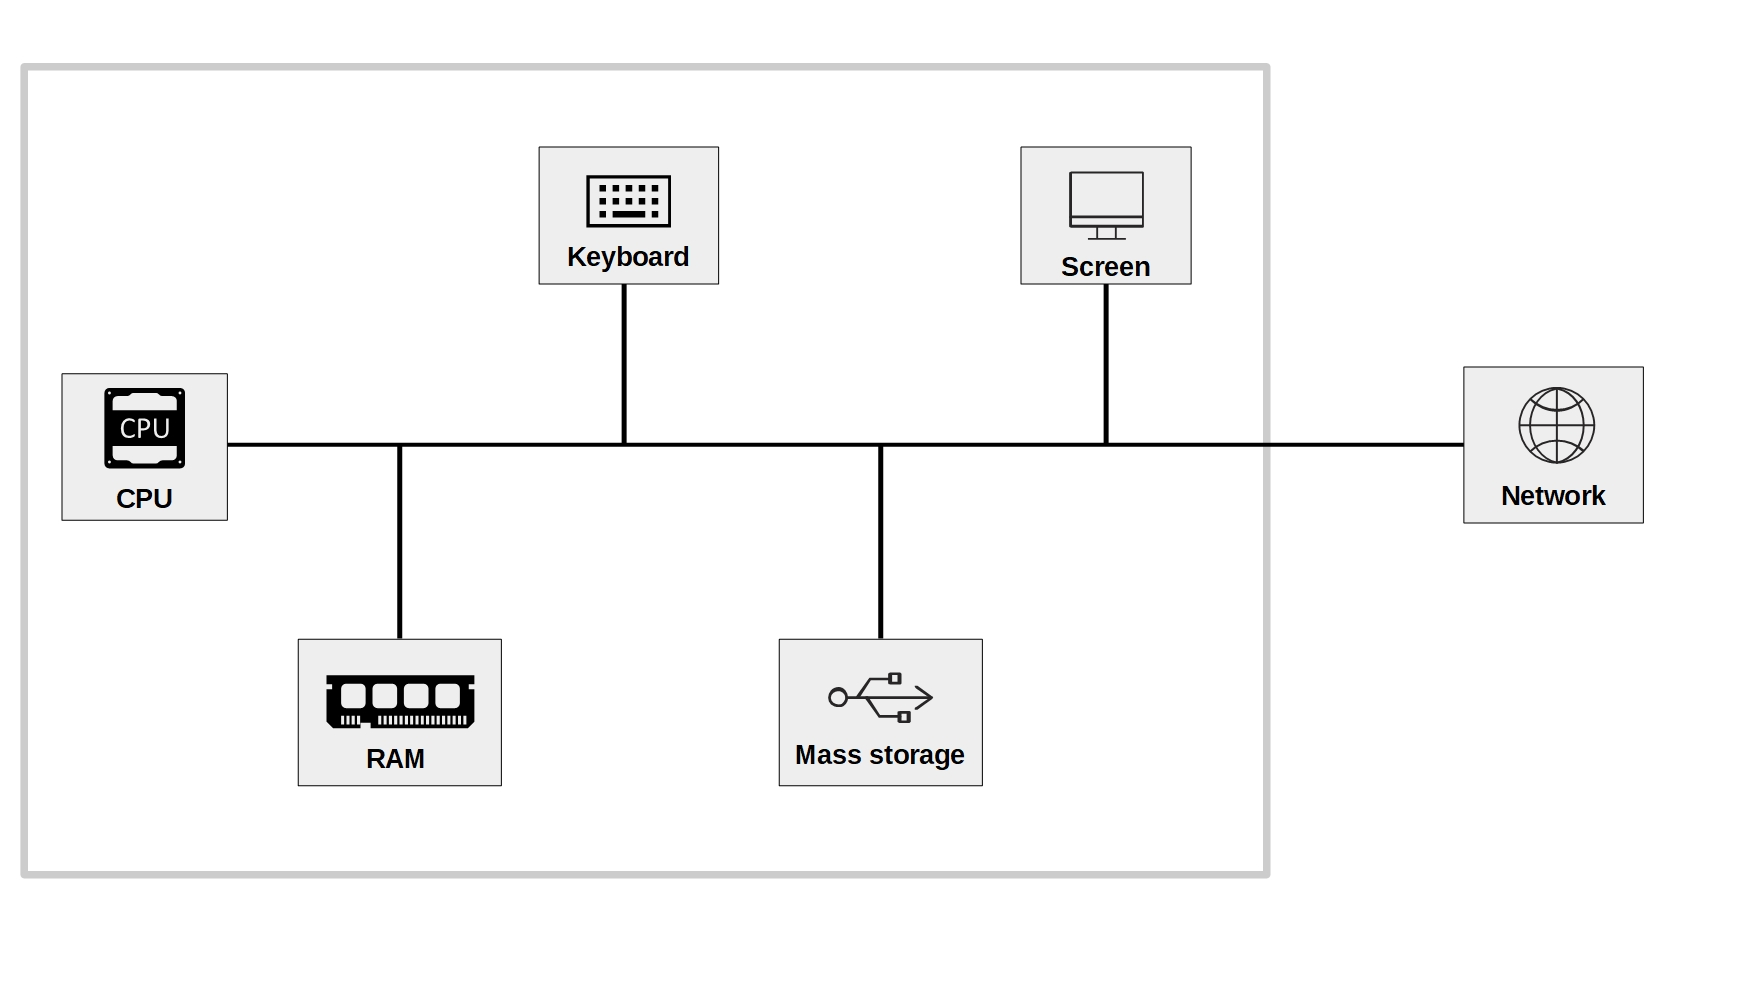
\includegraphics[width=0.6\linewidth]{img/03_script-hardware_w} 

}

\caption{Basic components of a standard computing environment.}\label{fig:components}
\end{figure}



\begin{itemize}
\item
  The component actually \emph{processing} data is the Central Processing Unit (CPU). When using R to process data, R commands are translated into complex combinations of a small set of basic operations which the \emph{CPU} then executes.
\item
  In order to work with data (e.g., in R), it first has to be loaded into the \emph{memory} of our computer. More specifically, into the Random Access Memory (\emph{RAM}). Typically, data is only loaded in the RAM as long as we work with it.
\item
  \emph{Mass Storage} refers to the type of computer memory we use to store data in the long run. This is what we call the \emph{hard drive} or \emph{hard disk}. In these days, the relevant hard disk is actually often not the one physically built into our computer but a hard disk `in the cloud' (built into a server to which we connect over the Internet).
\end{itemize}

Very simply put, the difference between `data analytics' and `Big Data analytics' is that in the latter case, the standard usage of one or several of these components fails or works very inefficiently because the amount of data overwhelms its normal capacity.

From this hardware-perspective, there are two basic strategies to cope with the situation that one of these components is overwhelmed by the amount of data:

\begin{itemize}
\tightlist
\item
  \emph{Scale up (`horizontal scaling')}: Extend the physical capacity of the affected component by building a system with large RAM shared between applications. This sounds like a trivial solution (`if RAM is too small, buy more RAM\ldots{}'), but in practice it can be very expensive.
\item
  \emph{Scale out (`vertical scaling')}: Distribute the workload over several computers (or separate components of a system).
\end{itemize}

From a software-perspective, there are many (context-specific) strategies that can help us to use the resources available more efficiently in order to process large amounts of data. In the context of computing statistics based on big data, this can involve:

\begin{itemize}
\tightlist
\item
  Implementing the computation of a given statistical procedure in a more efficient way (make better use of a given programming language or choose another programming language).
\item
  Choosing/implementing a more efficient statistical procedure/algorithm (see, e.g., the \emph{Uluru} algorithm).
\item
  At a lower level, improving how the system allocates resources.
\end{itemize}

\hypertarget{units-of-informationdata-storage}{%
\section{Units of information/data storage}\label{units-of-informationdata-storage}}

The smallest unit of information in computing/digital data is called a \emph{bit} (from \emph{bi}nary dig\emph{it}; abbrev. `b') and can take one of two (symbolic) values, either a \texttt{0} or a \texttt{1} (``off'' or ``on''). Consider, for example, the decimal number \texttt{139}. Written in the binary system, \texttt{139} corresponds to the binary number \texttt{10001011}. In order to store this number on a hard disk, we require a capacity of 8 bits, or one \emph{byte} (1 byte = 8 bits; abbrev. `B'). Historically, one byte encoded a single character of text (i.e., in the ASCII character encoding system). 4 bytes (or 32 bits) are called a \emph{word}. When thinking of a given data set in its raw/binary representation, we can simply think of it as a row of \texttt{0}s and \texttt{1}s, as illustrated in the following figure.

\begin{figure}

{\centering 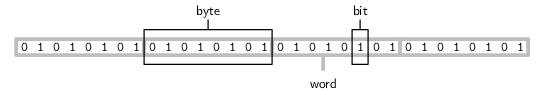
\includegraphics[width=0.5\linewidth]{img/03_store-bitbyteword} 

}

\caption{Writing data stored in RAM to a Mass Storage device (hard drive). Figure by \citet{murrell_2009} (licensed under CC BY-NC-SA 3.0 NZ).}\label{fig:bitbyteword}
\end{figure}



Bigger units for storage capacity usually build on bytes:

\begin{itemize}
\tightlist
\item
  \(1 \text{ kilobyte (KB)} = 1000^{1} \approx 2^{10} \text{ bytes}\)
\item
  \(1 \text{ megabyte (MB)} = 1000^{2} \approx 2^{20} \text{ bytes}\)
\item
  \(1 \text{ gigabyte (GB)} = 1000^{3} \approx 2^{30} \text{ bytes}\)
\item
  \(1 \text{ terabyte (TB)} = 1000^{4} \approx 2^{40} \text{ bytes}\)
\item
  \(1 \text{ petabyte (PB)} = 1000^{5} \approx 2^{50} \text{ bytes}\)
\item
  \(1 \text{ exabyte (EB)} = 1000^{6} \approx 2^{60} \text{ bytes}\)
\item
  \(1 \text{ zettabyte (ZB)} = 1000^{7} \approx 2^{70} \text{ bytes}\)
\end{itemize}

\[1 ZB = 1000000000000000000000\text{ bytes} = 1 \text{ billion terabytes} = 1 \text{ trillion gigabytes}.\]

\hypertarget{example-in-r-data-types-and-information-storage}{%
\subsection{Example in R: Data types and information storage}\label{example-in-r-data-types-and-information-storage}}

Given the fact that computers only understand \texttt{0}s and \texttt{1}s, different approaches are taken to map these digital values to other symbols or images (text, decimal numbers, pictures, etc.) that we humans can more easily make sense of. Regarding text and numbers, these mappings involve \emph{character encodings} (in which combinations of \texttt{0}s and \texttt{1}s represent a character in a specific alphabet) and \emph{data types}.

Let's illustrate the main concepts with the simple numerical example from above. When we see the decimal number \texttt{139} written somewhere, we know that it means `one-hundred-and-thirty-nine'. The fact that our computer is able to print \texttt{139} on the screen means that our computer can somehow map a sequence of \texttt{0}s and \texttt{1}s to the symbols \texttt{1}, \texttt{3}, and \texttt{9}. Depending on what we want to do with the data value \texttt{139} on our computer, there are different ways of how the computer can represent this value internally. Inter alia, we could load it into RAM as a \emph{string} (`text'/`character') or as an \emph{integer} (`natural number') or \emph{double} (numeric, floating point number). All of them can be printed on screen but only the latter two can be used for arithmetic computations. This concept can easily be illustrated in R.

We initiate a new variable with the value \texttt{139}. By using this syntax, R by default initiates the variable as an object of type \texttt{double}. We then can use this variable in arithmetic operations.

\begin{Shaded}
\begin{Highlighting}[]
\NormalTok{my\_number }\OtherTok{\textless{}{-}} \DecValTok{139}
\CommentTok{\# check the class}
\FunctionTok{typeof}\NormalTok{(my\_number)}
\end{Highlighting}
\end{Shaded}

\begin{verbatim}
## [1] "double"
\end{verbatim}

\begin{Shaded}
\begin{Highlighting}[]
\CommentTok{\# arithmetic}
\NormalTok{my\_number}\SpecialCharTok{*}\DecValTok{2}
\end{Highlighting}
\end{Shaded}

\begin{verbatim}
## [1] 278
\end{verbatim}

When we change the \emph{data type} to `character' (string) such operations are not possible.

\begin{Shaded}
\begin{Highlighting}[]
\CommentTok{\# change and check type/class}
\NormalTok{my\_number\_string }\OtherTok{\textless{}{-}} \FunctionTok{as.character}\NormalTok{(my\_number)}
\FunctionTok{typeof}\NormalTok{(my\_number\_string)}
\end{Highlighting}
\end{Shaded}

\begin{verbatim}
## [1] "character"
\end{verbatim}

\begin{Shaded}
\begin{Highlighting}[]
\CommentTok{\# try to multiply}
\NormalTok{my\_number\_string}\SpecialCharTok{*}\DecValTok{2}
\end{Highlighting}
\end{Shaded}

\begin{verbatim}
## Error in my_number_string * 2: non-numeric argument to binary operator
\end{verbatim}

If we change the variable to type \texttt{integer}, we can still use math operators.

\begin{Shaded}
\begin{Highlighting}[]
\CommentTok{\# change and check type/class}
\NormalTok{my\_number\_int }\OtherTok{\textless{}{-}} \FunctionTok{as.integer}\NormalTok{(my\_number)}
\FunctionTok{typeof}\NormalTok{(my\_number\_int)}
\end{Highlighting}
\end{Shaded}

\begin{verbatim}
## [1] "integer"
\end{verbatim}

\begin{Shaded}
\begin{Highlighting}[]
\CommentTok{\# arithmetics}
\NormalTok{my\_number\_int}\SpecialCharTok{*}\DecValTok{2}
\end{Highlighting}
\end{Shaded}

\begin{verbatim}
## [1] 278
\end{verbatim}

Having all variables in the right type is relevant for data analytics with all kind of sample sizes. However, given the fact that different data types have to be represented differently internally, different types might take up more or less memory and therefore substantially affect the performance when dealing with massive amounts of data.

We can illustrate this point with \texttt{object.size()}:

\begin{Shaded}
\begin{Highlighting}[]
\FunctionTok{object.size}\NormalTok{(}\StringTok{"139"}\NormalTok{)}
\end{Highlighting}
\end{Shaded}

\begin{verbatim}
## 112 bytes
\end{verbatim}

\begin{Shaded}
\begin{Highlighting}[]
\FunctionTok{object.size}\NormalTok{(}\DecValTok{139}\NormalTok{)}
\end{Highlighting}
\end{Shaded}

\begin{verbatim}
## 56 bytes
\end{verbatim}

\hypertarget{big-data-econometrics}{%
\section{Big Data econometrics}\label{big-data-econometrics}}

When thinking about how to approach a data analytics task based on large amounts of data, it is helpful to consider two key aspects concerning the computational burden involved. \((i)\) how is the statistic we have in mind computed. That is, what is the formal definition of the statistic (and how computationally demanding is it)? And \((ii)\), given a definition of the statistic, how does the program/software/language implement the computation thereof?

Regarding the former, we might realize that there is an alternative statistical procedure that would provide essentially the same output but that happens to be more efficient (here: computationally efficient in contrast to statistically efficient). The latter point is a question of how to efficiently implement the given statistical procedure in your computing environment (taking into consideration the computer's available resources: CPU, RAM, etc.).

Below, we look at both of these two aspects by means of illustrative examples.

\hypertarget{example-fast-least-squares-regression}{%
\section{Example: Fast least squares regression}\label{example-fast-least-squares-regression}}

As an illustration of how an alternative statistical procedure can speed up our analysis, we look at one such procedure that has recently been developed to estimate linear models when the classical OLS estimator is too computationally intense for very large samples: The \emph{Uluru} algorithm \citep{dhillon_2013}.

\hypertarget{ols-as-a-point-of-reference}{%
\subsection{OLS as a point of reference}\label{ols-as-a-point-of-reference}}

Recall the OLS estimator in matrix notation, given the linear model \(\mathbf{y}=\mathbf{X}\beta + \epsilon\):

\(\hat{\beta}_{OLS} = (\mathbf{X}^\intercal\mathbf{X})^{-1}\mathbf{X}^{\intercal}\mathbf{y}\).

In order to compute \(\hat{\beta}_{OLS}\), we have to compute \((\mathbf{X}^\intercal\mathbf{X})^{-1}\), which implies a computationally expensive matrix inversion.\footnote{The computational complexity of this is larger than \(O(n^{2})\). That is, for an input of size \(n\), the time needed to compute (or the number of operations needed) is \(n^2\).} If our data set is large, \(\mathbf{X}\) is large and the inversion can take up a lot of computation time. Moreover, the inversion and matrix multiplication to get \(\hat{\beta}_{OLS}\) needs a lot of memory. In practice, it might well be that the estimation of a linear model via OLS with the standard approach in R (\texttt{lm()}) brings a computer to its knees, as there is not enough RAM available.

To further illustrate the point, we implement the OLS estimator in R.

\begin{Shaded}
\begin{Highlighting}[]
\NormalTok{beta\_ols }\OtherTok{\textless{}{-}} 
     \ControlFlowTok{function}\NormalTok{(X, y) \{}
          
          \CommentTok{\# compute cross products and inverse}
\NormalTok{          XXi }\OtherTok{\textless{}{-}} \FunctionTok{solve}\NormalTok{(}\FunctionTok{crossprod}\NormalTok{(X,X))}
\NormalTok{          Xy }\OtherTok{\textless{}{-}} \FunctionTok{crossprod}\NormalTok{(X, y) }
          
          \FunctionTok{return}\NormalTok{( XXi  }\SpecialCharTok{\%*\%}\NormalTok{ Xy )}
\NormalTok{     \}}
\end{Highlighting}
\end{Shaded}

Now, we will test our OLS estimator function with a few (pseudo) random numbers in a Monte Carlo study. First, we set the sample size parameters \texttt{n} (how many observations shall our pseudo sample have?) and \texttt{p} (how many variables shall describe these observations?) and initiate the data set \texttt{X}.

\begin{Shaded}
\begin{Highlighting}[]
\CommentTok{\# set parameter values}
\NormalTok{n }\OtherTok{\textless{}{-}} \DecValTok{10000000}
\NormalTok{p }\OtherTok{\textless{}{-}} \DecValTok{4} 

\CommentTok{\# Generate sample based on Monte Carlo}
\CommentTok{\# generate a design matrix (\textasciitilde{} our \textquotesingle{}dataset\textquotesingle{}) with four variables and 10000 observations}
\NormalTok{X }\OtherTok{\textless{}{-}} \FunctionTok{matrix}\NormalTok{(}\FunctionTok{rnorm}\NormalTok{(n}\SpecialCharTok{*}\NormalTok{p, }\AttributeTok{mean =} \DecValTok{10}\NormalTok{), }\AttributeTok{ncol =}\NormalTok{ p)}
\CommentTok{\# add column for intercept}
\NormalTok{X }\OtherTok{\textless{}{-}} \FunctionTok{cbind}\NormalTok{(}\FunctionTok{rep}\NormalTok{(}\DecValTok{1}\NormalTok{, n), X)}
\end{Highlighting}
\end{Shaded}

Now we define how the real linear model looks like that we have in mind and compute the output \texttt{y} of this model, given the input \texttt{X}.\footnote{In reality we would not know this, of course. Acting as if we knew the real model is exactly the point of Monte Carlo studies. It allows us to analyze the properties of estimators by simulation.}

\begin{Shaded}
\begin{Highlighting}[]
\CommentTok{\# MC model}
\NormalTok{y }\OtherTok{\textless{}{-}} \DecValTok{2} \SpecialCharTok{+} \FloatTok{1.5}\SpecialCharTok{*}\NormalTok{X[,}\DecValTok{2}\NormalTok{] }\SpecialCharTok{+} \DecValTok{4}\SpecialCharTok{*}\NormalTok{X[,}\DecValTok{3}\NormalTok{] }\SpecialCharTok{{-}} \FloatTok{3.5}\SpecialCharTok{*}\NormalTok{X[,}\DecValTok{4}\NormalTok{] }\SpecialCharTok{+} \FloatTok{0.5}\SpecialCharTok{*}\NormalTok{X[,}\DecValTok{5}\NormalTok{] }\SpecialCharTok{+} \FunctionTok{rnorm}\NormalTok{(n)}
\end{Highlighting}
\end{Shaded}

Finally, we test our \texttt{beta\_ols} function.

\begin{Shaded}
\begin{Highlighting}[]
\CommentTok{\# apply the ols estimator}
\FunctionTok{beta\_ols}\NormalTok{(X, y)}
\end{Highlighting}
\end{Shaded}

\begin{verbatim}
##         [,1]
## [1,]  1.9897
## [2,]  1.5006
## [3,]  4.0005
## [4,] -3.4999
## [5,]  0.4998
\end{verbatim}

\hypertarget{the-uluru-algorithm-as-an-alternative-to-ols}{%
\subsection{The Uluru algorithm as an alternative to OLS}\label{the-uluru-algorithm-as-an-alternative-to-ols}}

Following \citet{dhillon_2013}, we implement a procedure to compute \(\hat{\beta}_{Uluru}\):

\[\hat{\beta}_{Uluru}=\hat{\beta}_{FS} + \hat{\beta}_{correct}\], where
\[\hat{\beta}_{FS} = (\mathbf{X}_{subs}^\intercal\mathbf{X}_{subs})^{-1}\mathbf{X}_{subs}^{\intercal}\mathbf{y}_{subs}\], and
\[\hat{\beta}_{correct}= \frac{n_{subs}}{n_{rem}} \cdot (\mathbf{X}_{subs}^\intercal\mathbf{X}_{subs})^{-1} \mathbf{X}_{rem}^{\intercal}\mathbf{R}_{rem}\], and
\[\mathbf{R}_{rem} = \mathbf{Y}_{rem} - \mathbf{X}_{rem}  \cdot \hat{\beta}_{FS}\].

The key idea behind this is that the computational bottleneck of the OLS estimator, the cross product and matrix inversion,\((\mathbf{X}^\intercal\mathbf{X})^{-1}\), is only computed on a sub-sample (\(X_{subs}\), etc.), not the entire data set. However, the remainder of the data set is also taken into consideration (in order to correct a bias arising from the sub-sampling). Again, we implement the estimator in R to further illustrate this point.

\begin{Shaded}
\begin{Highlighting}[]
\NormalTok{beta\_uluru }\OtherTok{\textless{}{-}}
     \ControlFlowTok{function}\NormalTok{(X\_subs, y\_subs, X\_rem, y\_rem) \{}
          
          \CommentTok{\# compute beta\_fs (this is simply OLS applied to the subsample)}
\NormalTok{          XXi\_subs }\OtherTok{\textless{}{-}} \FunctionTok{solve}\NormalTok{(}\FunctionTok{crossprod}\NormalTok{(X\_subs, X\_subs))}
\NormalTok{          Xy\_subs }\OtherTok{\textless{}{-}} \FunctionTok{crossprod}\NormalTok{(X\_subs, y\_subs)}
\NormalTok{          b\_fs }\OtherTok{\textless{}{-}}\NormalTok{ XXi\_subs  }\SpecialCharTok{\%*\%}\NormalTok{ Xy\_subs}
          
          \CommentTok{\# compute \textbackslash{}mathbf\{R\}\_\{rem\}}
\NormalTok{          R\_rem }\OtherTok{\textless{}{-}}\NormalTok{ y\_rem }\SpecialCharTok{{-}}\NormalTok{ X\_rem }\SpecialCharTok{\%*\%}\NormalTok{ b\_fs}
          
          \CommentTok{\# compute \textbackslash{}hat\{\textbackslash{}beta\}\_\{correct\}}
\NormalTok{          b\_correct }\OtherTok{\textless{}{-}}\NormalTok{ (}\FunctionTok{nrow}\NormalTok{(X\_subs)}\SpecialCharTok{/}\NormalTok{(}\FunctionTok{nrow}\NormalTok{(X\_rem))) }\SpecialCharTok{*}\NormalTok{ XXi\_subs }\SpecialCharTok{\%*\%} \FunctionTok{crossprod}\NormalTok{(X\_rem, R\_rem)}

          \CommentTok{\# beta uluru       }
          \FunctionTok{return}\NormalTok{(b\_fs }\SpecialCharTok{+}\NormalTok{ b\_correct)}
\NormalTok{     \}}
\end{Highlighting}
\end{Shaded}

Test it with the same input as above:

\begin{Shaded}
\begin{Highlighting}[]
\CommentTok{\# set size of subsample}
\NormalTok{n\_subs }\OtherTok{\textless{}{-}} \DecValTok{1000}
\CommentTok{\# select subsample and remainder}
\NormalTok{n\_obs }\OtherTok{\textless{}{-}} \FunctionTok{nrow}\NormalTok{(X)}
\NormalTok{X\_subs }\OtherTok{\textless{}{-}}\NormalTok{ X[1L}\SpecialCharTok{:}\NormalTok{n\_subs,]}
\NormalTok{y\_subs }\OtherTok{\textless{}{-}}\NormalTok{ y[1L}\SpecialCharTok{:}\NormalTok{n\_subs]}
\NormalTok{X\_rem }\OtherTok{\textless{}{-}}\NormalTok{ X[(n\_subs}\SpecialCharTok{+}\NormalTok{1L)}\SpecialCharTok{:}\NormalTok{n\_obs,]}
\NormalTok{y\_rem }\OtherTok{\textless{}{-}}\NormalTok{ y[(n\_subs}\SpecialCharTok{+}\NormalTok{1L)}\SpecialCharTok{:}\NormalTok{n\_obs]}

\CommentTok{\# apply the uluru estimator}
\FunctionTok{beta\_uluru}\NormalTok{(X\_subs, y\_subs, X\_rem, y\_rem)}
\end{Highlighting}
\end{Shaded}

\begin{verbatim}
##         [,1]
## [1,]  1.9244
## [2,]  1.5015
## [3,]  4.0059
## [4,] -3.5000
## [5,]  0.5004
\end{verbatim}

This looks quite good already. Let's have a closer look with a little Monte Carlo study. The aim of the simulation study is to visualize the difference between the classical OLS approach and the \emph{Uluru} algorithm with regard to bias and time complexity if we increase the sub-sample size in \emph{Uluru}. For simplicity, we only look at the first estimated coefficient \(\beta_{1}\).

\begin{Shaded}
\begin{Highlighting}[]
\CommentTok{\# define subsamples}
\NormalTok{n\_subs\_sizes }\OtherTok{\textless{}{-}} \FunctionTok{seq}\NormalTok{(}\AttributeTok{from =} \DecValTok{1000}\NormalTok{, }\AttributeTok{to =} \DecValTok{500000}\NormalTok{, }\AttributeTok{by=}\DecValTok{10000}\NormalTok{)}
\NormalTok{n\_runs }\OtherTok{\textless{}{-}} \FunctionTok{length}\NormalTok{(n\_subs\_sizes)}
\CommentTok{\# compute uluru result, stop time}
\NormalTok{mc\_results }\OtherTok{\textless{}{-}} \FunctionTok{rep}\NormalTok{(}\ConstantTok{NA}\NormalTok{, n\_runs)}
\NormalTok{mc\_times }\OtherTok{\textless{}{-}} \FunctionTok{rep}\NormalTok{(}\ConstantTok{NA}\NormalTok{, n\_runs)}
\ControlFlowTok{for}\NormalTok{ (i }\ControlFlowTok{in} \DecValTok{1}\SpecialCharTok{:}\NormalTok{n\_runs) \{}
     \CommentTok{\# set size of subsample}
\NormalTok{     n\_subs }\OtherTok{\textless{}{-}}\NormalTok{ n\_subs\_sizes[i]}
     \CommentTok{\# select subsample and remainder}
\NormalTok{     n\_obs }\OtherTok{\textless{}{-}} \FunctionTok{nrow}\NormalTok{(X)}
\NormalTok{     X\_subs }\OtherTok{\textless{}{-}}\NormalTok{ X[1L}\SpecialCharTok{:}\NormalTok{n\_subs,]}
\NormalTok{     y\_subs }\OtherTok{\textless{}{-}}\NormalTok{ y[1L}\SpecialCharTok{:}\NormalTok{n\_subs]}
\NormalTok{     X\_rem }\OtherTok{\textless{}{-}}\NormalTok{ X[(n\_subs}\SpecialCharTok{+}\NormalTok{1L)}\SpecialCharTok{:}\NormalTok{n\_obs,]}
\NormalTok{     y\_rem }\OtherTok{\textless{}{-}}\NormalTok{ y[(n\_subs}\SpecialCharTok{+}\NormalTok{1L)}\SpecialCharTok{:}\NormalTok{n\_obs]}
     
\NormalTok{     mc\_results[i] }\OtherTok{\textless{}{-}} \FunctionTok{beta\_uluru}\NormalTok{(X\_subs, y\_subs, X\_rem, y\_rem)[}\DecValTok{2}\NormalTok{] }\CommentTok{\# the first element is the intercept}
\NormalTok{     mc\_times[i] }\OtherTok{\textless{}{-}} \FunctionTok{system.time}\NormalTok{(}\FunctionTok{beta\_uluru}\NormalTok{(X\_subs, y\_subs, X\_rem, y\_rem))[}\DecValTok{3}\NormalTok{]}
     
\NormalTok{\}}

\CommentTok{\# compute ols results and ols time}
\NormalTok{ols\_time }\OtherTok{\textless{}{-}} \FunctionTok{system.time}\NormalTok{(}\FunctionTok{beta\_ols}\NormalTok{(X, y))}
\NormalTok{ols\_res }\OtherTok{\textless{}{-}} \FunctionTok{beta\_ols}\NormalTok{(X, y)[}\DecValTok{2}\NormalTok{]}
\end{Highlighting}
\end{Shaded}

Let's visualize the comparison with OLS.

\begin{Shaded}
\begin{Highlighting}[]
\CommentTok{\# load packages}
\FunctionTok{library}\NormalTok{(ggplot2)}

\CommentTok{\# prepare data to plot}
\NormalTok{plotdata }\OtherTok{\textless{}{-}} \FunctionTok{data.frame}\NormalTok{(}\AttributeTok{beta1 =}\NormalTok{ mc\_results,}
                       \AttributeTok{time\_elapsed =}\NormalTok{ mc\_times,}
                       \AttributeTok{subs\_size =}\NormalTok{ n\_subs\_sizes)}
\end{Highlighting}
\end{Shaded}

First, let's look at the time used estimate the linear model.

\begin{Shaded}
\begin{Highlighting}[]
\FunctionTok{ggplot}\NormalTok{(plotdata, }\FunctionTok{aes}\NormalTok{(}\AttributeTok{x =}\NormalTok{ subs\_size, }\AttributeTok{y =}\NormalTok{ time\_elapsed)) }\SpecialCharTok{+}
     \FunctionTok{geom\_point}\NormalTok{(}\AttributeTok{color=}\StringTok{"darkgreen"}\NormalTok{) }\SpecialCharTok{+} 
     \FunctionTok{geom\_hline}\NormalTok{(}\AttributeTok{yintercept =}\NormalTok{ ols\_time[}\DecValTok{3}\NormalTok{],}
                \AttributeTok{color =} \StringTok{"red"}\NormalTok{, }
                \AttributeTok{size =} \DecValTok{1}\NormalTok{) }\SpecialCharTok{+}
     \FunctionTok{theme\_minimal}\NormalTok{() }\SpecialCharTok{+}
     \FunctionTok{ylab}\NormalTok{(}\StringTok{"Time elapsed"}\NormalTok{) }\SpecialCharTok{+}
     \FunctionTok{xlab}\NormalTok{(}\StringTok{"Subsample size"}\NormalTok{)}
\end{Highlighting}
\end{Shaded}

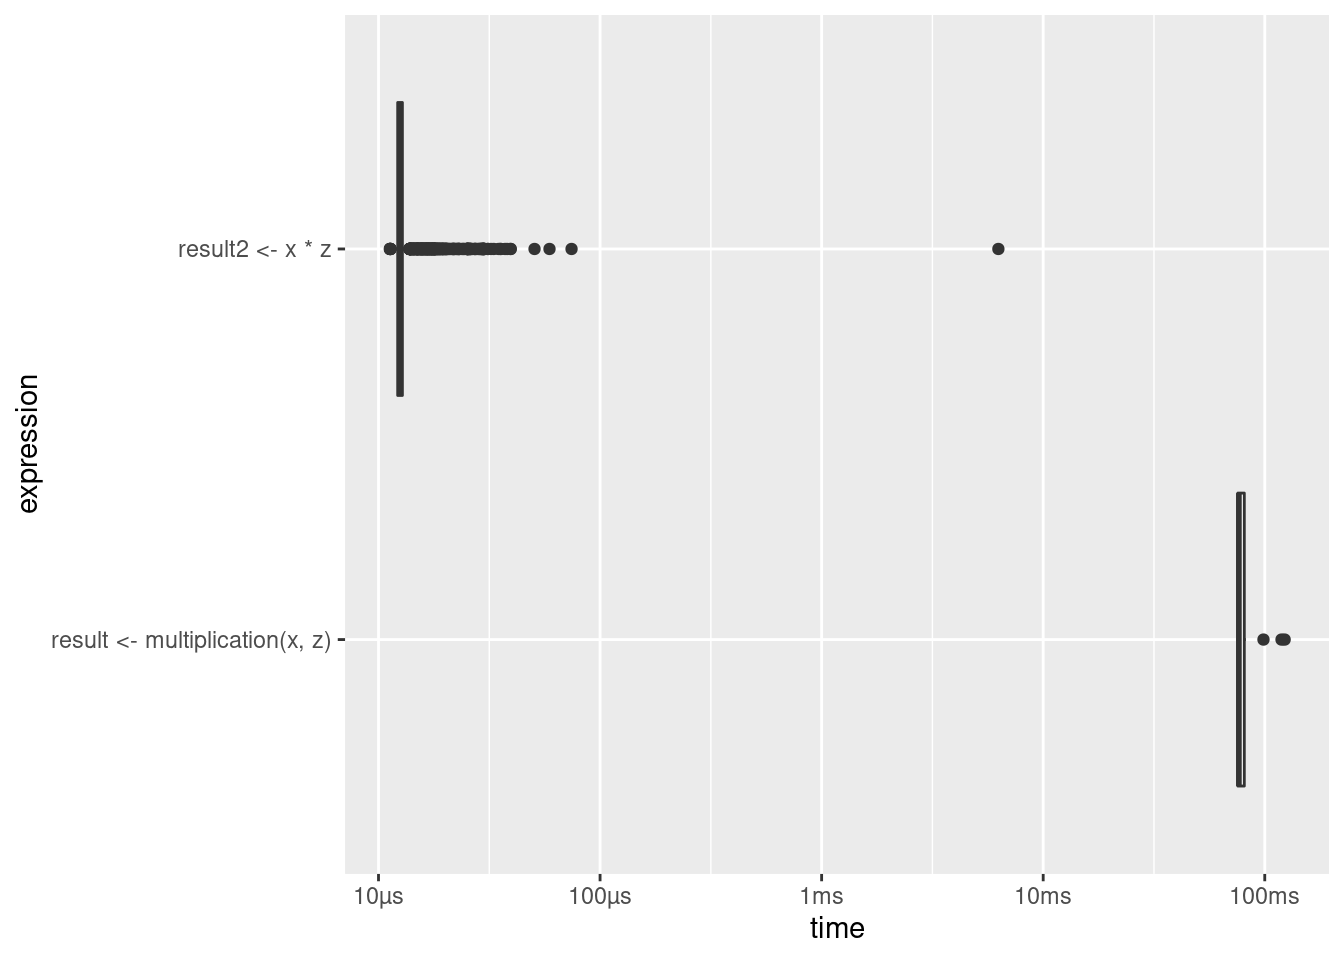
\includegraphics{bigdata_files/figure-latex/unnamed-chunk-28-1.pdf}

The horizontal red line indicates the computation time for estimation via OLS, the green points indicate the computation time for the estimation via the Ulruru algorithm. Note that even for large sub-samples, the computation time is substantially lower than for OLS.

Finally, let's have a look at how close the results are to OLS.

\begin{Shaded}
\begin{Highlighting}[]
\FunctionTok{ggplot}\NormalTok{(plotdata, }\FunctionTok{aes}\NormalTok{(}\AttributeTok{x =}\NormalTok{ subs\_size, }\AttributeTok{y =}\NormalTok{ beta1)) }\SpecialCharTok{+}
     \FunctionTok{geom\_hline}\NormalTok{(}\AttributeTok{yintercept =}\NormalTok{ ols\_res,}
                \AttributeTok{color =} \StringTok{"red"}\NormalTok{, }
                \AttributeTok{size =} \DecValTok{1}\NormalTok{) }\SpecialCharTok{+}
       \FunctionTok{geom\_hline}\NormalTok{(}\AttributeTok{yintercept =} \FloatTok{1.5}\NormalTok{,}
                \AttributeTok{color =} \StringTok{"green"}\NormalTok{,}
                \AttributeTok{size =} \DecValTok{1}\NormalTok{) }\SpecialCharTok{+}
     \FunctionTok{geom\_point}\NormalTok{(}\AttributeTok{color=}\StringTok{"darkgreen"}\NormalTok{) }\SpecialCharTok{+} 

     \FunctionTok{theme\_minimal}\NormalTok{() }\SpecialCharTok{+}
     \FunctionTok{ylab}\NormalTok{(}\StringTok{"Estimated coefficient"}\NormalTok{) }\SpecialCharTok{+}
     \FunctionTok{xlab}\NormalTok{(}\StringTok{"Subsample size"}\NormalTok{)}
\end{Highlighting}
\end{Shaded}

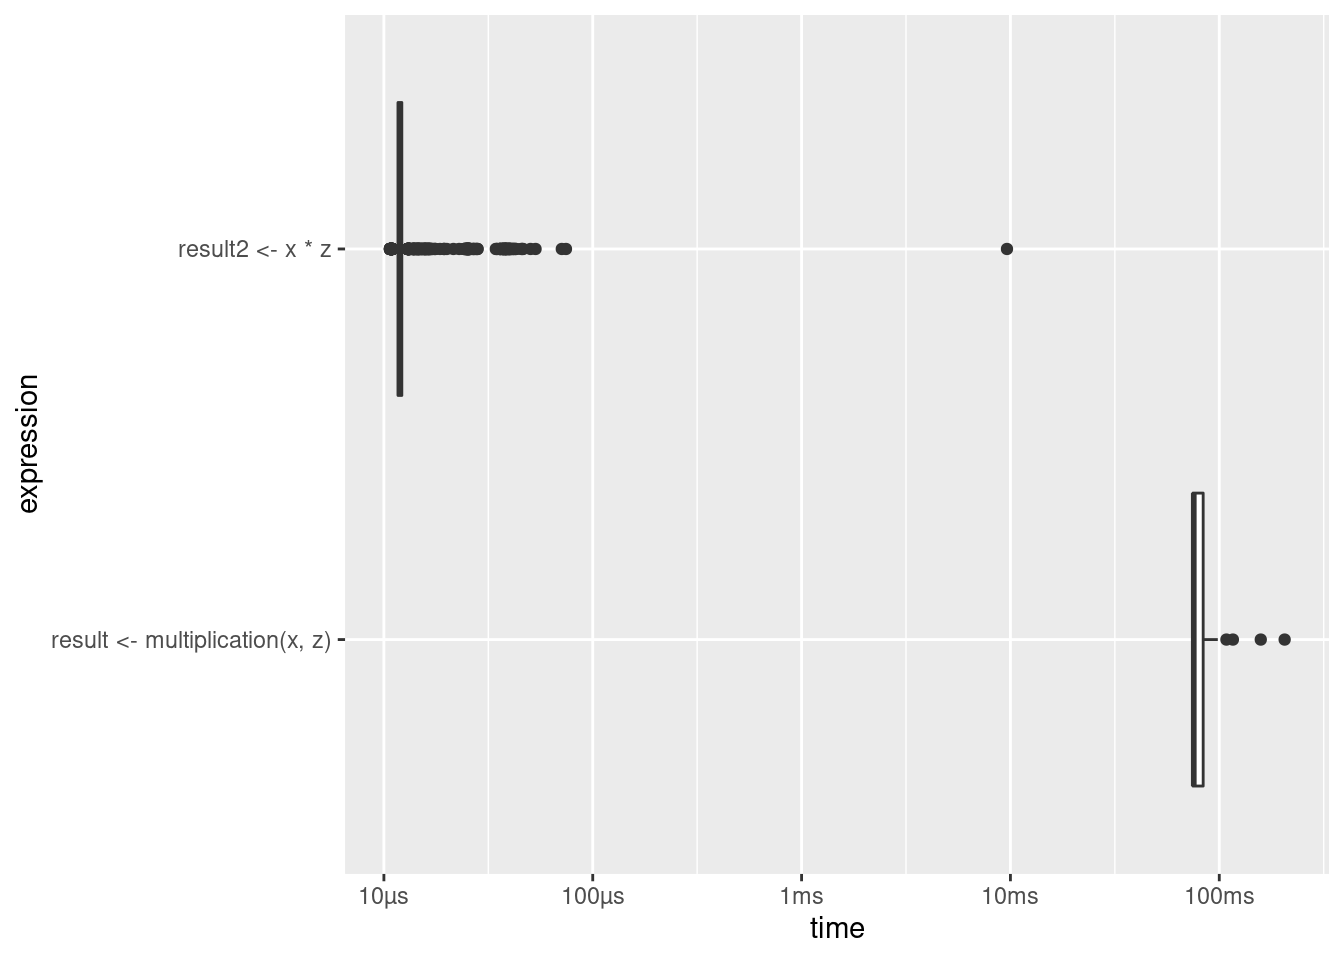
\includegraphics{bigdata_files/figure-latex/unnamed-chunk-29-1.pdf}

The horizontal red line indicates the size of the estimated coefficient, when using OLS. The horizontal green line indicates the size of the actual coefficient. The green points indicate the size of the same coefficient estimated by the Uluru algorithm for different sub-sample sizes. Note that even relatively small sub-samples already deliver estimates very close to the OLS estimates.

\hypertarget{resource-allocation}{%
\chapter{Resource allocation}\label{resource-allocation}}

When optimizing the performance of an analytics program processing large amounts of data, it is useful to differentiate between the efficient allocation of computational (CPU) power, and the allocation of RAM (and mass storage).\footnote{In many data analysis tasks the two are, of course, intertwined. However, keeping both aspects in mind when optimizing an analytics program helps to choose the right tools.} Below, we will look at both aspects in turn.

\hypertarget{case-study-parallel-processing}{%
\section{Case study: Parallel processing}\label{case-study-parallel-processing}}

In this example, we estimate a simple regression model that aims to assess racial discrimination in the context of police stops.\footnote{Note that this example aims to illustrate a point about computation in an applied econometrics context. It does not make any argument about identification or the broader research question whatsoever.} The example is based on the `Minneapolis Police Department 2017 Stop Dataset', containing data on nearly all stops made by the Minneapolis Police Department for the year 2017.

We start with importing the data into R.

\begin{Shaded}
\begin{Highlighting}[]
\NormalTok{url }\OtherTok{\textless{}{-}} \StringTok{"https://vincentarelbundock.github.io/Rdatasets/csv/carData/MplsStops.csv"}
\NormalTok{stopdata }\OtherTok{\textless{}{-}}\NormalTok{ data.table}\SpecialCharTok{::}\FunctionTok{fread}\NormalTok{(url) }
\end{Highlighting}
\end{Shaded}

We specify a simple linear probability model that aims to test whether a person identified as `white' is less likely to have her vehicle searched when stopped by the police. In order to take into account level-differences between different police precincts, we add precinct-indicators to the regression specification

First, let's remove observations with missing entries (\texttt{NA}) and code our main explanatory variable and the dependent variable.

\begin{Shaded}
\begin{Highlighting}[]
\CommentTok{\# remove incomplete obs}
\NormalTok{stopdata }\OtherTok{\textless{}{-}} \FunctionTok{na.omit}\NormalTok{(stopdata)}
\CommentTok{\# code dependent var}
\NormalTok{stopdata}\SpecialCharTok{$}\NormalTok{vsearch }\OtherTok{\textless{}{-}} \DecValTok{0}
\NormalTok{stopdata}\SpecialCharTok{$}\NormalTok{vsearch[stopdata}\SpecialCharTok{$}\NormalTok{vehicleSearch}\SpecialCharTok{==}\StringTok{"YES"}\NormalTok{] }\OtherTok{\textless{}{-}} \DecValTok{1}
\CommentTok{\# code explanatory var}
\NormalTok{stopdata}\SpecialCharTok{$}\NormalTok{white }\OtherTok{\textless{}{-}} \DecValTok{0}
\NormalTok{stopdata}\SpecialCharTok{$}\NormalTok{white[stopdata}\SpecialCharTok{$}\NormalTok{race}\SpecialCharTok{==}\StringTok{"White"}\NormalTok{] }\OtherTok{\textless{}{-}} \DecValTok{1}
\end{Highlighting}
\end{Shaded}

We specify our baseline model as follows.

\begin{Shaded}
\begin{Highlighting}[]
\NormalTok{model }\OtherTok{\textless{}{-}}\NormalTok{ vsearch }\SpecialCharTok{\textasciitilde{}}\NormalTok{ white }\SpecialCharTok{+} \FunctionTok{factor}\NormalTok{(policePrecinct)}
\end{Highlighting}
\end{Shaded}

And estimate the linear probability model via OLS (the \texttt{lm} function).

\begin{Shaded}
\begin{Highlighting}[]
\NormalTok{fit }\OtherTok{\textless{}{-}} \FunctionTok{lm}\NormalTok{(model, stopdata)}
\FunctionTok{summary}\NormalTok{(fit)}
\end{Highlighting}
\end{Shaded}

\begin{verbatim}
## 
## Call:
## lm(formula = model, data = stopdata)
## 
## Residuals:
##     Min      1Q  Median      3Q     Max 
## -0.1394 -0.0633 -0.0547 -0.0423  0.9773 
## 
## Coefficients:
##                         Estimate Std. Error t value
## (Intercept)              0.05473    0.00515   10.62
## white                   -0.01955    0.00446   -4.38
## factor(policePrecinct)2  0.00856    0.00676    1.27
## factor(policePrecinct)3  0.00341    0.00648    0.53
## factor(policePrecinct)4  0.08464    0.00623   13.58
## factor(policePrecinct)5 -0.01246    0.00637   -1.96
##                         Pr(>|t|)    
## (Intercept)              < 2e-16 ***
## white                    1.2e-05 ***
## factor(policePrecinct)2     0.21    
## factor(policePrecinct)3     0.60    
## factor(policePrecinct)4  < 2e-16 ***
## factor(policePrecinct)5     0.05 .  
## ---
## Signif. codes:  
## 0 '***' 0.001 '**' 0.01 '*' 0.05 '.' 0.1 ' ' 1
## 
## Residual standard error: 0.254 on 19078 degrees of freedom
## Multiple R-squared:  0.025,  Adjusted R-squared:  0.0248 
## F-statistic: 97.9 on 5 and 19078 DF,  p-value: <2e-16
\end{verbatim}

A potential problem with this approach (and there might be many more in this simple example) is that observations stemming from different police precincts might be correlated over time. If that is the case, we likely underestimate the coefficient's standard errors. There is a standard approach to compute estimates for so-called \emph{cluster-robust} standard errors which would take the problem of correlation over time within clusters into consideration (and deliver a more conservative estimate of the SEs). However, this approach only works well if the number of clusters in the data is roughly 50 or more. Here we only have 5.

The alternative approach is to compute bootstrapped clustered standard errors. That is, we apply the \href{https://en.wikipedia.org/wiki/Bootstrapping_(statistics)}{bootstrap resampling procedure} at the cluster level. Specifically, we draw \(B\) samples (with replacement), estimate and record for each bootstrap-sample the coefficient vector, and then estimate \(SE_{boot}\) based on the standard deviation of all respective estimated coefficient values.

\begin{Shaded}
\begin{Highlighting}[]
\CommentTok{\# load packages}
\FunctionTok{library}\NormalTok{(data.table)}
\CommentTok{\# set the \textquotesingle{}seed\textquotesingle{} for random numbers (makes the example reproducible)}
\FunctionTok{set.seed}\NormalTok{(}\DecValTok{2}\NormalTok{)}

\CommentTok{\# set number of bootstrap iterations}
\NormalTok{B }\OtherTok{\textless{}{-}} \DecValTok{10}
\CommentTok{\# get selection of precincts}
\NormalTok{precincts }\OtherTok{\textless{}{-}} \FunctionTok{unique}\NormalTok{(stopdata}\SpecialCharTok{$}\NormalTok{policePrecinct)}
\CommentTok{\# container for coefficients}
\NormalTok{boot\_coefs }\OtherTok{\textless{}{-}} \FunctionTok{matrix}\NormalTok{(}\ConstantTok{NA}\NormalTok{, }\AttributeTok{nrow =}\NormalTok{ B, }\AttributeTok{ncol =} \DecValTok{2}\NormalTok{)}
\CommentTok{\# draw bootstrap samples, estimate model for each sample}
\ControlFlowTok{for}\NormalTok{ (i }\ControlFlowTok{in} \DecValTok{1}\SpecialCharTok{:}\NormalTok{B) \{}
     
     \CommentTok{\# draw sample of precincts (cluster level)}
\NormalTok{     precincts\_i }\OtherTok{\textless{}{-}} \FunctionTok{sample}\NormalTok{(precincts, }\AttributeTok{size =} \DecValTok{5}\NormalTok{, }\AttributeTok{replace =} \ConstantTok{TRUE}\NormalTok{)}
     \CommentTok{\# get observations}
\NormalTok{     bs\_i }\OtherTok{\textless{}{-}} \FunctionTok{lapply}\NormalTok{(precincts\_i, }\ControlFlowTok{function}\NormalTok{(x) stopdata[stopdata}\SpecialCharTok{$}\NormalTok{policePrecinct}\SpecialCharTok{==}\NormalTok{x,])}
\NormalTok{     bs\_i }\OtherTok{\textless{}{-}} \FunctionTok{rbindlist}\NormalTok{(bs\_i)}
     
     \CommentTok{\# estimate model and record coefficients}
\NormalTok{     boot\_coefs[i,] }\OtherTok{\textless{}{-}} \FunctionTok{coef}\NormalTok{(}\FunctionTok{lm}\NormalTok{(model, bs\_i))[}\DecValTok{1}\SpecialCharTok{:}\DecValTok{2}\NormalTok{] }\CommentTok{\# ignore FE{-}coefficients}
\NormalTok{\}}
\end{Highlighting}
\end{Shaded}

Finally, let's compute \(SE_{boot}\).

\begin{Shaded}
\begin{Highlighting}[]
\NormalTok{se\_boot }\OtherTok{\textless{}{-}} \FunctionTok{apply}\NormalTok{(boot\_coefs, }
                 \AttributeTok{MARGIN =} \DecValTok{2}\NormalTok{,}
                 \AttributeTok{FUN =}\NormalTok{ sd)}
\NormalTok{se\_boot}
\end{Highlighting}
\end{Shaded}

\begin{verbatim}
## [1] 0.004043 0.004690
\end{verbatim}

Note that even with a very small \(B\), computing \(SE_{boot}\) takes up some time to compute. When setting \(B\) to over 500, computation time will be substantial. Also note that running this code does hardly use up more memory than the very simple approach without bootstrapping (after all, in each bootstrap iteration the data set used to estimate the model is approximately the same size as the original data set). There is little we can do to improve the script's performance regarding memory. However we can tell R how to allocate CPU resources more efficiently to handle that many regression estimates.

Particularly, we can make use of the fact that most modern computing environments (such as a laptop) have CPUs with several \emph{cores}. We can exploit this fact by instructing the computer to run the computations \emph{in parallel} (simultaneously computing on several cores). The following code is a parallel implementation of our bootstrap procedure which does exactly that.

\begin{Shaded}
\begin{Highlighting}[]
\CommentTok{\# install.packages("doSNOW", "parallel")}
\CommentTok{\# load packages for parallel processing}
\FunctionTok{library}\NormalTok{(doSNOW)}

\CommentTok{\# get the number of cores available}
\NormalTok{ncores }\OtherTok{\textless{}{-}}\NormalTok{ parallel}\SpecialCharTok{::}\FunctionTok{detectCores}\NormalTok{()}
\CommentTok{\# set cores for parallel processing}
\NormalTok{ctemp }\OtherTok{\textless{}{-}} \FunctionTok{makeCluster}\NormalTok{(ncores) }\CommentTok{\# }
\FunctionTok{registerDoSNOW}\NormalTok{(ctemp)}


\CommentTok{\# set number of bootstrap iterations}
\NormalTok{B }\OtherTok{\textless{}{-}} \DecValTok{10}
\CommentTok{\# get selection of precincts}
\NormalTok{precincts }\OtherTok{\textless{}{-}} \FunctionTok{unique}\NormalTok{(stopdata}\SpecialCharTok{$}\NormalTok{policePrecinct)}
\CommentTok{\# container for coefficients}
\NormalTok{boot\_coefs }\OtherTok{\textless{}{-}} \FunctionTok{matrix}\NormalTok{(}\ConstantTok{NA}\NormalTok{, }\AttributeTok{nrow =}\NormalTok{ B, }\AttributeTok{ncol =} \DecValTok{2}\NormalTok{)}

\CommentTok{\# bootstrapping in parallel}
\NormalTok{boot\_coefs }\OtherTok{\textless{}{-}} 
     \FunctionTok{foreach}\NormalTok{(}\AttributeTok{i =} \DecValTok{1}\SpecialCharTok{:}\NormalTok{B, }\AttributeTok{.combine =}\NormalTok{ rbind, }\AttributeTok{.packages=}\StringTok{"data.table"}\NormalTok{) }\SpecialCharTok{\%dopar\%}\NormalTok{ \{}
          
          \CommentTok{\# draw sample of precincts (cluster level)}
\NormalTok{          precincts\_i }\OtherTok{\textless{}{-}} \FunctionTok{sample}\NormalTok{(precincts, }\AttributeTok{size =} \DecValTok{5}\NormalTok{, }\AttributeTok{replace =} \ConstantTok{TRUE}\NormalTok{)}
          \CommentTok{\# get observations}
\NormalTok{          bs\_i }\OtherTok{\textless{}{-}} \FunctionTok{lapply}\NormalTok{(precincts\_i, }\ControlFlowTok{function}\NormalTok{(x) stopdata[stopdata}\SpecialCharTok{$}\NormalTok{policePrecinct}\SpecialCharTok{==}\NormalTok{x,])}
\NormalTok{          bs\_i }\OtherTok{\textless{}{-}} \FunctionTok{rbindlist}\NormalTok{(bs\_i)}
          
          \CommentTok{\# estimate model and record coefficients}
          \FunctionTok{coef}\NormalTok{(}\FunctionTok{lm}\NormalTok{(model, bs\_i))[}\DecValTok{1}\SpecialCharTok{:}\DecValTok{2}\NormalTok{] }\CommentTok{\# ignore FE{-}coefficients}
      
\NormalTok{     \}}


\CommentTok{\# be a good citizen and stop the snow clusters}
\FunctionTok{stopCluster}\NormalTok{(}\AttributeTok{cl =}\NormalTok{ ctemp)}
\end{Highlighting}
\end{Shaded}

As a last step, we compute again \(SE_{boot}\).

\begin{Shaded}
\begin{Highlighting}[]
\NormalTok{se\_boot }\OtherTok{\textless{}{-}} \FunctionTok{apply}\NormalTok{(boot\_coefs, }
                 \AttributeTok{MARGIN =} \DecValTok{2}\NormalTok{,}
                 \AttributeTok{FUN =}\NormalTok{ sd)}
\NormalTok{se\_boot}
\end{Highlighting}
\end{Shaded}

\begin{verbatim}
## (Intercept)       white 
##    0.004193    0.004334
\end{verbatim}

\hypertarget{case-study-memory-allocation}{%
\section{Case study: Memory allocation}\label{case-study-memory-allocation}}

Consider the first steps of a data pipeline in R. The first part of our script to import and clean the data looks as follows.

\begin{Shaded}
\begin{Highlighting}[]
\DocumentationTok{\#\#\#\#\#\#\#\#\#\#\#\#\#\#\#\#\#\#\#\#\#\#\#\#\#\#\#\#\#\#\#\#\#\#\#\#\#\#\#\#\#\#\#\#\#\#\#\#\#\#\#\#\#\#\#\#\#\#\#}
\CommentTok{\# Big Data Statistics: Flights data import and preparation}
\CommentTok{\#}
\CommentTok{\# U. Matter, January 2019}
\DocumentationTok{\#\#\#\#\#\#\#\#\#\#\#\#\#\#\#\#\#\#\#\#\#\#\#\#\#\#\#\#\#\#\#\#\#\#\#\#\#\#\#\#\#\#\#\#\#\#\#\#\#\#\#\#\#\#\#\#\#\#\#}

\CommentTok{\# SET UP {-}{-}{-}{-}{-}{-}{-}{-}{-}{-}{-}{-}{-}{-}{-}{-}{-}}

\CommentTok{\# fix variables}
\NormalTok{DATA\_PATH }\OtherTok{\textless{}{-}} \StringTok{"materials/data/flights.csv"}

\CommentTok{\# DATA IMPORT {-}{-}{-}{-}{-}{-}{-}{-}{-}{-}{-}{-}{-}{-}{-}{-}}
\NormalTok{flights }\OtherTok{\textless{}{-}} \FunctionTok{read.csv}\NormalTok{(DATA\_PATH)}

\CommentTok{\# DATA PREPARATION {-}{-}{-}{-}{-}{-}{-}{-}}
\NormalTok{flights }\OtherTok{\textless{}{-}}\NormalTok{ flights[,}\SpecialCharTok{{-}}\DecValTok{1}\SpecialCharTok{:{-}}\DecValTok{3}\NormalTok{]}
\end{Highlighting}
\end{Shaded}

When running this script, we notice that some of the steps need a noticable amount of time to process. Moreover, while none of these steps obviously involves a lot of computation (such as a matrix inversion or numerical optimization), it quite likely involves memory allocation. We first read data into RAM (allocated to R by our operating system). It turns out that there are different ways to allocate RAM when reading data from a CSV file. Depending on the amount of data to be read in, one or the other approach might be faster. We first investigate the RAM allocation in R with \texttt{mem\_change()} and \texttt{mem\_used()}.

\begin{Shaded}
\begin{Highlighting}[]
\CommentTok{\# SET UP {-}{-}{-}{-}{-}{-}{-}{-}{-}{-}{-}{-}{-}{-}{-}{-}{-}}

\CommentTok{\# fix variables}
\NormalTok{DATA\_PATH }\OtherTok{\textless{}{-}} \StringTok{"data/flights.csv"}
\CommentTok{\# load packages}
\FunctionTok{library}\NormalTok{(pryr) }
\end{Highlighting}
\end{Shaded}

\begin{verbatim}
## Registered S3 method overwritten by 'pryr':
##   method      from
##   print.bytes Rcpp
\end{verbatim}

\begin{verbatim}
## 
## Attaching package: 'pryr'
\end{verbatim}

\begin{verbatim}
## The following object is masked from 'package:data.table':
## 
##     address
\end{verbatim}

\begin{Shaded}
\begin{Highlighting}[]
\CommentTok{\# check how much memory is used by R (overall)}
\FunctionTok{mem\_used}\NormalTok{()}
\end{Highlighting}
\end{Shaded}

\begin{verbatim}
## 1.04 GB
\end{verbatim}

\begin{Shaded}
\begin{Highlighting}[]
\CommentTok{\# check the change in memory due to each step}

\CommentTok{\# DATA IMPORT {-}{-}{-}{-}{-}{-}{-}{-}{-}{-}{-}{-}{-}{-}{-}{-}}
\FunctionTok{mem\_change}\NormalTok{(flights }\OtherTok{\textless{}{-}} \FunctionTok{read.csv}\NormalTok{(DATA\_PATH))}
\end{Highlighting}
\end{Shaded}

\begin{verbatim}
## 33.2 MB
\end{verbatim}

\begin{Shaded}
\begin{Highlighting}[]
\CommentTok{\# DATA PREPARATION {-}{-}{-}{-}{-}{-}{-}{-}}
\NormalTok{flights }\OtherTok{\textless{}{-}}\NormalTok{ flights[,}\SpecialCharTok{{-}}\DecValTok{1}\SpecialCharTok{:{-}}\DecValTok{3}\NormalTok{]}

\CommentTok{\# check how much memory is used by R now}
\FunctionTok{mem\_used}\NormalTok{()}
\end{Highlighting}
\end{Shaded}

\begin{verbatim}
## 1.07 GB
\end{verbatim}

The last result is kind of interesting. The object \texttt{flights} must have been larger right after importing it than at the end of the script. We have thrown out several variables, after all. Why does R still use that much memory? R does by default not `clean up' memory unless it is really necessary (meaning no more memory is available). In this case, R has still way more memory available from the operating system, thus there is no need to `collect the garbage' yet. However, we can force R to collect the garbage on the spot with \texttt{gc()}. This can be helpful to better keep track of the memory needed by an analytics script.

\begin{Shaded}
\begin{Highlighting}[]
\FunctionTok{gc}\NormalTok{()}
\end{Highlighting}
\end{Shaded}

\begin{verbatim}
##             used  (Mb) gc trigger   (Mb)  max used
## Ncells   1080420  57.8    2100091  112.2   1889052
## Vcells 126631854 966.2  213476124 1628.7 211148494
##          (Mb)
## Ncells  100.9
## Vcells 1611.0
\end{verbatim}

Now, let's see how we can improve the performance of this script with regard to memory allocation. Most memory is allocated when importing the file. Obviously, any improvement of the script must still result in importing all the data. However, there are different ways to read data into RAM. \texttt{read.csv()} reads all lines of a csv file consecutively. In contrast, \texttt{data.table::fread()} first `maps' the data file into memory and only then actually reads it in line by line. This involves an additional initial step, but the larger the file, the less relevant is this first step with regard to the total time needed to read all the data into memory. By switching on the \texttt{verbose} option, we can actually see what \texttt{fread} is doing.

\begin{Shaded}
\begin{Highlighting}[]
\CommentTok{\# load packages}
\FunctionTok{library}\NormalTok{(data.table)}

\CommentTok{\# DATA IMPORT {-}{-}{-}{-}{-}{-}{-}{-}{-}{-}{-}{-}{-}{-}{-}{-}}
\NormalTok{flights }\OtherTok{\textless{}{-}} \FunctionTok{fread}\NormalTok{(DATA\_PATH, }\AttributeTok{verbose =} \ConstantTok{TRUE}\NormalTok{)}
\end{Highlighting}
\end{Shaded}

\begin{verbatim}
##   OpenMP version (_OPENMP)       201511
##   omp_get_num_procs()            12
##   R_DATATABLE_NUM_PROCS_PERCENT  unset (default 50)
##   R_DATATABLE_NUM_THREADS        unset
##   R_DATATABLE_THROTTLE           unset (default 1024)
##   omp_get_thread_limit()         2147483647
##   omp_get_max_threads()          12
##   OMP_THREAD_LIMIT               unset
##   OMP_NUM_THREADS                unset
##   RestoreAfterFork               true
##   data.table is using 6 threads with throttle==1024. See ?setDTthreads.
## freadR.c has been passed a filename: data/flights.csv
## [01] Check arguments
##   Using 6 threads (omp_get_max_threads()=12, nth=6)
##   NAstrings = [<<NA>>]
##   None of the NAstrings look like numbers.
##   show progress = 0
##   0/1 column will be read as integer
## [02] Opening the file
##   Opening file data/flights.csv
##   File opened, size = 29.53MB (30960660 bytes).
##   Memory mapped ok
## [03] Detect and skip BOM
## [04] Arrange mmap to be \0 terminated
##   \n has been found in the input and different lines can end with different line endings (e.g. mixed \n and \r\n in one file). This is common and ideal.
## [05] Skipping initial rows if needed
##   Positioned on line 1 starting: <<year,month,day,dep_time,sched_>>
## [06] Detect separator, quoting rule, and ncolumns
##   Detecting sep automatically ...
##   sep=','  with 100 lines of 19 fields using quote rule 0
##   Detected 19 columns on line 1. This line is either column names or first data row. Line starts as: <<year,month,day,dep_time,sched_>>
##   Quote rule picked = 0
##   fill=false and the most number of columns found is 19
## [07] Detect column types, good nrow estimate and whether first row is column names
##   Number of sampling jump points = 100 because (30960659 bytes from row 1 to eof) / (2 * 8882 jump0size) == 1742
##   Type codes (jump 000)    : 555555555C5CCC5555B  Quote rule 0
##   Type codes (jump 100)    : 555555555C5CCC5555B  Quote rule 0
##   'header' determined to be true due to column 1 containing a string on row 1 and a lower type (int32) in the rest of the 10048 sample rows
##   =====
##   Sampled 10048 rows (handled \n inside quoted fields) at 101 jump points
##   Bytes from first data row on line 2 to the end of last row: 30960501
##   Line length: mean=92.03 sd=3.56 min=68 max=98
##   Estimated number of rows: 30960501 / 92.03 = 336403
##   Initial alloc = 370043 rows (336403 + 9%) using bytes/max(mean-2*sd,min) clamped between [1.1*estn, 2.0*estn]
##   =====
## [08] Assign column names
## [09] Apply user overrides on column types
##   After 0 type and 0 drop user overrides : 555555555C5CCC5555B
## [10] Allocate memory for the datatable
##   Allocating 19 column slots (19 - 0 dropped) with 370043 rows
## [11] Read the data
##   jumps=[0..30), chunk_size=1032016, total_size=30960501
## Read 336776 rows x 19 columns from 29.53MB (30960660 bytes) file in 00:00.062 wall clock time
## [12] Finalizing the datatable
##   Type counts:
##         14 : int32     '5'
##          1 : float64   'B'
##          4 : string    'C'
## =============================
##    0.000s (  0%) Memory map 0.029GB file
##    0.003s (  4%) sep=',' ncol=19 and header detection
##    0.000s (  0%) Column type detection using 10048 sample rows
##    0.001s (  1%) Allocation of 370043 rows x 19 cols (0.033GB) of which 336776 ( 91%) rows used
##    0.059s ( 94%) Reading 30 chunks (0 swept) of 0.984MB (each chunk 11225 rows) using 6 threads
##    +    0.015s ( 25%) Parse to row-major thread buffers (grown 0 times)
##    +    0.027s ( 43%) Transpose
##    +    0.017s ( 27%) Waiting
##    0.000s (  0%) Rereading 0 columns due to out-of-sample type exceptions
##    0.062s        Total
\end{verbatim}

Let's put it all together and look at the memory changes and usage. For a fair comparison, we first have to delete \texttt{flights} and collect the garbage with \texttt{gc()}.

\begin{Shaded}
\begin{Highlighting}[]
\CommentTok{\# SET UP {-}{-}{-}{-}{-}{-}{-}{-}{-}{-}{-}{-}{-}{-}{-}{-}{-}}

\CommentTok{\# fix variables}
\NormalTok{DATA\_PATH }\OtherTok{\textless{}{-}} \StringTok{"data/flights.csv"}
\CommentTok{\# load packages}
\FunctionTok{library}\NormalTok{(pryr) }
\FunctionTok{library}\NormalTok{(data.table)}

\CommentTok{\# housekeeping}
\NormalTok{flights }\OtherTok{\textless{}{-}} \ConstantTok{NULL}
\FunctionTok{gc}\NormalTok{()}
\end{Highlighting}
\end{Shaded}

\begin{verbatim}
##             used  (Mb) gc trigger   (Mb)  max used
## Ncells   1069455  57.2    2100091  112.2   1889052
## Vcells 123466113 942.0  213476124 1628.7 211148494
##          (Mb)
## Ncells  100.9
## Vcells 1611.0
\end{verbatim}

\begin{Shaded}
\begin{Highlighting}[]
\CommentTok{\# check the change in memory due to each step}

\CommentTok{\# DATA IMPORT {-}{-}{-}{-}{-}{-}{-}{-}{-}{-}{-}{-}{-}{-}{-}{-}}
\FunctionTok{mem\_change}\NormalTok{(flights }\OtherTok{\textless{}{-}} \FunctionTok{fread}\NormalTok{(DATA\_PATH))}
\end{Highlighting}
\end{Shaded}

\begin{verbatim}
## 35.8 MB
\end{verbatim}

\hypertarget{beyond-memory}{%
\section{Beyond memory}\label{beyond-memory}}

In the previous example we have inspected how RAM is allocated to store objects in the R computing environment. But what if all RAM of our computer is not enough to store all the data we want to analyze?

Modern operating systems have a way to dealing with such a situation. Once all RAM is used up by the currently running programs, the OS allocates parts of the memory back to the hard-disk which then works as \emph{virtual memory}. The following figure illustrates this point.

\begin{figure}

{\centering 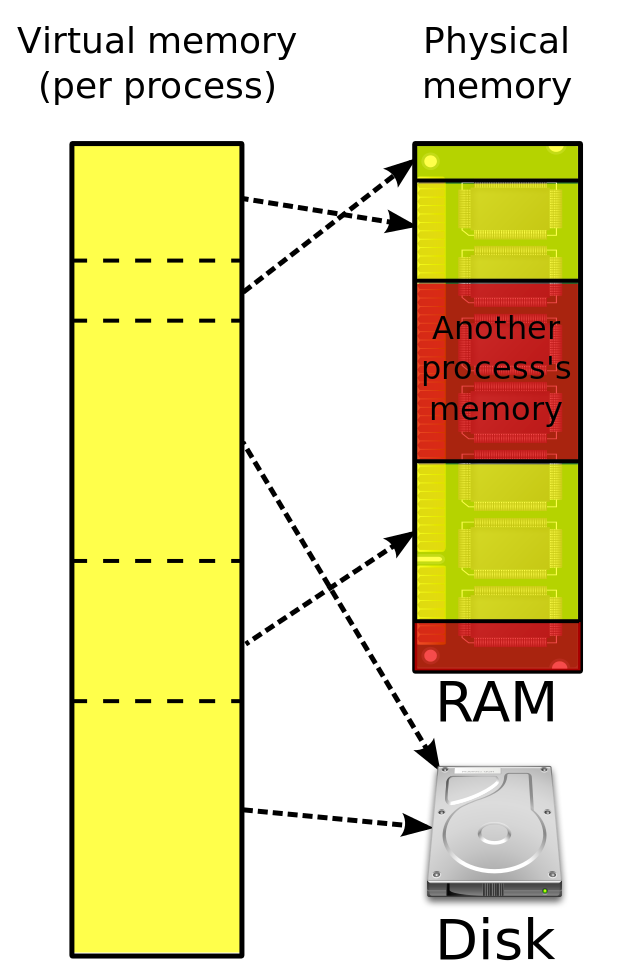
\includegraphics[width=0.3\linewidth]{img/03_virtualmemory} 

}

\caption{Virtual memory. Figure by Ehamberg (CC BY-SA 3.0).}\label{fig:vm}
\end{figure}



For example, when we implement an R-script that imports one file after the other into the R environment, ignoring the RAM capacity of our computer, the OS will start \emph{paging} data to the virtual memory. This happens `under the hood' without explicit instructions by the user. We quite likely notice that the computer slows down a lot when this happens.

While this default usage of virtual memory by the OS is helpful to run several applications at the same time, each taking up a moderate amount of memory, it is not a really useful tool for processing large amounts of data in one application (R). However, the underlying idea of using both RAM and Mass storage simultaneously in order to cope with a lack of memory is very useful in the context of big data analytics.

Several R packages have been developed that exploit the idea behind virtual memory explicitly for analyzing large amounts of data. The basic idea behind these packages is to map a data set to the hard disk when loading it into R. The actual data values are stored in chunks on the hard-disk, while the structure/metadata of the data set is loaded into R. See this week's slide set as well as \citet{walkowiak_2016}, Chapter 3 for more details and example code.

\hypertarget{advanced-r-programming}{%
\chapter{Advanced R Programming}\label{advanced-r-programming}}

\hypertarget{r-tools-to-investigate-performanceresource-allocation}{%
\section{R-tools to investigate performance/resource allocation}\label{r-tools-to-investigate-performanceresource-allocation}}

\begin{longtable}[]{@{}
  >{\raggedright\arraybackslash}p{(\columnwidth - 4\tabcolsep) * \real{0.13}}
  >{\raggedright\arraybackslash}p{(\columnwidth - 4\tabcolsep) * \real{0.16}}
  >{\raggedright\arraybackslash}p{(\columnwidth - 4\tabcolsep) * \real{0.71}}@{}}
\toprule
package & function & purpose \\
\midrule
\endhead
\texttt{utils} & \texttt{object.size()} & Provides an estimate of the memory that is being used to store an R object. \\
\texttt{pryr} & \texttt{object\_size()} & Works similarly to \texttt{object.size()}, but counts more accurately and includes the size of environments. \\
\texttt{pryr} & \texttt{compare\_size()} & Makes it easy to compare the output of object\_size and object.size. \\
\texttt{pryr} & \texttt{mem\_used()} & Returns the total amount of memory (in megabytes) currently used by R. \\
\texttt{pryr} & \texttt{mem\_change()} & Shows the change in memory (in megabytes) before and after running code. \\
\texttt{base} & \texttt{system.time()} & Returns CPU (and other) times that an R expression used. \\
\texttt{microbenchmark} & \texttt{microbenchmark()} & Highly accurate timing of R expression evaluation. \\
\texttt{bench} & \texttt{mark()} & Benchmark a series of functions. \\
\texttt{profvis} & \texttt{profvis()} & Profiles an R expression and visualizes the profiling data (usage of memory, time elapsed, etc.). \\
\bottomrule
\end{longtable}

\hypertarget{r-tools-to-investigate-structures-and-types}{%
\section{R-tools to investigate structures and types}\label{r-tools-to-investigate-structures-and-types}}

\begin{longtable}[]{@{}
  >{\raggedright\arraybackslash}p{(\columnwidth - 4\tabcolsep) * \real{0.13}}
  >{\raggedright\arraybackslash}p{(\columnwidth - 4\tabcolsep) * \real{0.16}}
  >{\raggedright\arraybackslash}p{(\columnwidth - 4\tabcolsep) * \real{0.71}}@{}}
\toprule
package & function & purpose \\
\midrule
\endhead
\texttt{utils} & \texttt{str()} & Compactly display the structure of an arbitrary R object. \\
\texttt{base} & \texttt{class()} & Prints the class(es) of an R object. \\
\texttt{base} & \texttt{typeof()} & Determines the (R-internal) type or storage mode of an object. \\
\bottomrule
\end{longtable}

\hypertarget{data-types-and-memorystorage}{%
\section{Data types and memory/storage}\label{data-types-and-memorystorage}}

Data loaded into RAM can be interpreted differently by R depending on the data \emph{type}. Some operators or functions in R only accept data of a specific type as arguments. For example, we can store the numeric values \texttt{1.5} and \texttt{3} in the variables \texttt{a} and \texttt{b}, respectively.

\begin{Shaded}
\begin{Highlighting}[]
\NormalTok{a }\OtherTok{\textless{}{-}} \FloatTok{1.5}
\NormalTok{b }\OtherTok{\textless{}{-}} \DecValTok{3}
\NormalTok{a }\SpecialCharTok{+}\NormalTok{ b}
\end{Highlighting}
\end{Shaded}

\begin{verbatim}
## [1] 4.5
\end{verbatim}

R interprets this data as type \texttt{double} (class `numeric'):

\begin{Shaded}
\begin{Highlighting}[]
\FunctionTok{typeof}\NormalTok{(a)}
\end{Highlighting}
\end{Shaded}

\begin{verbatim}
## [1] "double"
\end{verbatim}

\begin{Shaded}
\begin{Highlighting}[]
\FunctionTok{class}\NormalTok{(a)}
\end{Highlighting}
\end{Shaded}

\begin{verbatim}
## [1] "numeric"
\end{verbatim}

\begin{Shaded}
\begin{Highlighting}[]
\FunctionTok{object.size}\NormalTok{(a)}
\end{Highlighting}
\end{Shaded}

\begin{verbatim}
## 56 bytes
\end{verbatim}

If, however, we define \texttt{a} and \texttt{b} as follows, R will interpret the values stored in \texttt{a} and \texttt{b} as text (\texttt{character}).

\begin{Shaded}
\begin{Highlighting}[]
\NormalTok{a }\OtherTok{\textless{}{-}} \StringTok{"1.5"}
\NormalTok{b }\OtherTok{\textless{}{-}} \StringTok{"3"}
\NormalTok{a }\SpecialCharTok{+}\NormalTok{ b}
\end{Highlighting}
\end{Shaded}

\begin{Shaded}
\begin{Highlighting}[]
\FunctionTok{typeof}\NormalTok{(a)}
\end{Highlighting}
\end{Shaded}

\begin{verbatim}
## [1] "double"
\end{verbatim}

\begin{Shaded}
\begin{Highlighting}[]
\FunctionTok{class}\NormalTok{(a)}
\end{Highlighting}
\end{Shaded}

\begin{verbatim}
## [1] "numeric"
\end{verbatim}

\begin{Shaded}
\begin{Highlighting}[]
\FunctionTok{object.size}\NormalTok{(a)}
\end{Highlighting}
\end{Shaded}

\begin{verbatim}
## 56 bytes
\end{verbatim}

Note that the symbols \texttt{1.5} take up more or less memory depending on the data-type they are stored in. This directly links to how data/information is stored/represented in binary code, which in turn is reflected in how much memory is used to store these symbols in an object as well as what we can do with it.

\hypertarget{data-structures}{%
\section{Data structures}\label{data-structures}}

For now, we have only looked at individual bytes of data. An entire data set can consist of gigabytes of data and contain both text and numeric values. R provides several classes of objects providing different data structures. Both the choice of data types and data structures to store data in can affect how much memory is needed to contain a dataset in RAM.

\hypertarget{vectors-vs-factors-in-r}{%
\subsection{Vectors vs Factors in R}\label{vectors-vs-factors-in-r}}

Vectors are collections of values of the same type. They can contain either all numeric values or all character values.

\begin{figure}

{\centering 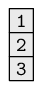
\includegraphics[width=0.05\linewidth]{img/02_numvec} 

}

\caption{Illustration of a numeric vector (symbolic). Figure by \citet{murrell_2009} (licensed under CC BY-NC-SA 3.0 NZ).}\label{fig:numvec}
\end{figure}



For example, we can initiate a character vector containing information on the home towns of persons participating in a survey.

\begin{Shaded}
\begin{Highlighting}[]
\NormalTok{hometown }\OtherTok{\textless{}{-}} \FunctionTok{c}\NormalTok{(}\StringTok{"St.Gallen"}\NormalTok{, }\StringTok{"Basel"}\NormalTok{, }\StringTok{"St.Gallen"}\NormalTok{)}
\NormalTok{hometown}
\end{Highlighting}
\end{Shaded}

\begin{verbatim}
## [1] "St.Gallen" "Basel"     "St.Gallen"
\end{verbatim}

\begin{Shaded}
\begin{Highlighting}[]
\FunctionTok{object.size}\NormalTok{(hometown)}
\end{Highlighting}
\end{Shaded}

\begin{verbatim}
## 200 bytes
\end{verbatim}

Unlike in the data types example above, it would likely be not that practical to store these values as type \texttt{numeric} to save memory. R would not know how to translate these strings into floating point numbers. Alternatively, we could think of a correspondence table that assigns a numeric (id) code to each unique town name in the data set. This way we would save memory but it would mean additional effort to work with the data. Fortunately, basic R already implements exactly this idea in a user-friendly way in a data-structure called \texttt{factor}.

Factors are sets of categories. Thus, the values come from a fixed set of possible values.

\begin{figure}

{\centering 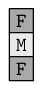
\includegraphics[width=0.05\linewidth]{img/02_factor} 

}

\caption{Illustration of a factor (symbolic). Figure by \citet{murrell_2009} (licensed under CC BY-NC-SA 3.0 NZ).}\label{fig:factor}
\end{figure}



Considering the same example as above, we can store the same information in an object of type class \texttt{factor}.

\begin{Shaded}
\begin{Highlighting}[]
\NormalTok{hometown\_f }\OtherTok{\textless{}{-}} \FunctionTok{factor}\NormalTok{(}\FunctionTok{c}\NormalTok{(}\StringTok{"St.Gallen"}\NormalTok{, }\StringTok{"Basel"}\NormalTok{, }\StringTok{"St.Gallen"}\NormalTok{))}
\NormalTok{hometown\_f}
\end{Highlighting}
\end{Shaded}

\begin{verbatim}
## [1] St.Gallen Basel     St.Gallen
## Levels: Basel St.Gallen
\end{verbatim}

\begin{Shaded}
\begin{Highlighting}[]
\FunctionTok{object.size}\NormalTok{(hometown\_f)}
\end{Highlighting}
\end{Shaded}

\begin{verbatim}
## 584 bytes
\end{verbatim}

At first sight, the fact that \texttt{hometown\_f} takes up more memory than its character vector sibling seems odd. But, we have encountered this kind of `paradox' before. Again, the more sophisticated approach involves an `overhead' (here not in terms of computing time but in terms of structure encoded in an object). \texttt{hometown\_f} has more `structure' (i.e., a mapping of numbers to `factor levels'/category labels). This additional structure is also information that needs to be stored somewhere. As in previous examples of this `overhead costs', this disadvantage is diminishing with larger data sets:

\begin{Shaded}
\begin{Highlighting}[]
\CommentTok{\# create a large character vector}
\NormalTok{hometown\_large }\OtherTok{\textless{}{-}} \FunctionTok{rep}\NormalTok{(hometown, }\AttributeTok{times =} \DecValTok{1000}\NormalTok{)}
\CommentTok{\# and the same content as factor}
\NormalTok{hometown\_large\_f }\OtherTok{\textless{}{-}} \FunctionTok{factor}\NormalTok{(hometown\_large)}
\CommentTok{\# compare size}
\FunctionTok{object.size}\NormalTok{(hometown\_large)}
\end{Highlighting}
\end{Shaded}

\begin{verbatim}
## 24168 bytes
\end{verbatim}

\begin{Shaded}
\begin{Highlighting}[]
\FunctionTok{object.size}\NormalTok{(hometown\_large\_f)}
\end{Highlighting}
\end{Shaded}

\begin{verbatim}
## 12568 bytes
\end{verbatim}

\hypertarget{matricesarrays}{%
\subsection{Matrices/Arrays}\label{matricesarrays}}

Matrices are two-dimensional collections of values, arrays higher-dimensional collections of values, of the same type.

\begin{figure}

{\centering 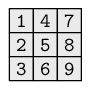
\includegraphics[width=0.1\linewidth]{img/02_matrix} 

}

\caption{Illustration of a numeric matrix (symbolic). Figure by \citet{murrell_2009} (licensed under CC BY-NC-SA 3.0 NZ).}\label{fig:matrix}
\end{figure}



For example, we can initiate a three-row/two-column numeric matrix as follows.

\begin{Shaded}
\begin{Highlighting}[]
\NormalTok{my\_matrix }\OtherTok{\textless{}{-}} \FunctionTok{matrix}\NormalTok{(}\FunctionTok{c}\NormalTok{(}\DecValTok{1}\NormalTok{,}\DecValTok{2}\NormalTok{,}\DecValTok{3}\NormalTok{,}\DecValTok{4}\NormalTok{,}\DecValTok{5}\NormalTok{,}\DecValTok{6}\NormalTok{), }\AttributeTok{nrow =} \DecValTok{3}\NormalTok{)}
\NormalTok{my\_matrix}
\end{Highlighting}
\end{Shaded}

\begin{verbatim}
##      [,1] [,2]
## [1,]    1    4
## [2,]    2    5
## [3,]    3    6
\end{verbatim}

And a three-dimensional numeric array as follows.

\begin{Shaded}
\begin{Highlighting}[]
\NormalTok{my\_array }\OtherTok{\textless{}{-}} \FunctionTok{array}\NormalTok{(}\FunctionTok{c}\NormalTok{(}\DecValTok{1}\NormalTok{,}\DecValTok{2}\NormalTok{,}\DecValTok{3}\NormalTok{,}\DecValTok{4}\NormalTok{,}\DecValTok{5}\NormalTok{,}\DecValTok{6}\NormalTok{), }\AttributeTok{dim =} \DecValTok{3}\NormalTok{)}
\NormalTok{my\_array}
\end{Highlighting}
\end{Shaded}

\begin{verbatim}
## [1] 1 2 3
\end{verbatim}

\hypertarget{data-frames-tibbles-and-data-tables}{%
\subsection{Data frames, tibbles, and data tables}\label{data-frames-tibbles-and-data-tables}}

Recall that data frames are the typical representation of a (table-like) data set in R. Each column can contain a vector of a given data type (or a factor), but all columns need to be of identical length. Thus in the context of data analysis, we would say that each row of a data frame contains an observation, and each column contains a characteristic of this observation.

\begin{figure}

{\centering 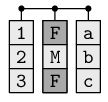
\includegraphics[width=0.1\linewidth]{img/02_df} 

}

\caption{Illustration of a data frame (symbolic). Figure by \citet{murrell_2009} (licensed under CC BY-NC-SA 3.0 NZ).}\label{fig:df}
\end{figure}



The historical implementation of data frames in R is not very comfortable to work with large data sets.\footnote{In the early days of R this was not really an issue because data sets that are rather large by today's standards (in the Gigabytes) could not have been handled properly by normal computers anyhow (due to a lack of RAM).} Several newer implementations of the data-frame concept in R aim to make data processing faster. One is called \texttt{tibbles}, implemented and used in the \texttt{tidyverse} packages. The other is called \texttt{data\ table}, implemented in the \texttt{data.table}-package. In this course we will focus on the \texttt{data.table}-package.

Here is how we define a \texttt{data.table} in R:

\begin{Shaded}
\begin{Highlighting}[]
\CommentTok{\# load package}
\FunctionTok{library}\NormalTok{(data.table)}
\CommentTok{\# initiate a data.table}
\NormalTok{dt }\OtherTok{\textless{}{-}} \FunctionTok{data.table}\NormalTok{(}\AttributeTok{person =} \FunctionTok{c}\NormalTok{(}\StringTok{"Alice"}\NormalTok{, }\StringTok{"Ben"}\NormalTok{),}
                 \AttributeTok{age =} \FunctionTok{c}\NormalTok{(}\DecValTok{50}\NormalTok{, }\DecValTok{30}\NormalTok{),}
                 \AttributeTok{gender =} \FunctionTok{c}\NormalTok{(}\StringTok{"f"}\NormalTok{, }\StringTok{"m"}\NormalTok{))}
\NormalTok{dt}
\end{Highlighting}
\end{Shaded}

\begin{verbatim}
##    person age gender
## 1:  Alice  50      f
## 2:    Ben  30      m
\end{verbatim}

\hypertarget{lists}{%
\subsection{Lists}\label{lists}}

Similar to data frames and data tables, lists can contain different types of data in each element. For example, a list could contain different other lists, data frames, and vectors with differing numbers of elements.

\begin{figure}

{\centering 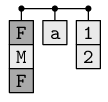
\includegraphics[width=0.1\linewidth]{img/02_list} 

}

\caption{Illustration of a data frame (symbolic). Figure by \citet{murrell_2009} (licensed under CC BY-NC-SA 3.0 NZ).}\label{fig:list}
\end{figure}



This flexibility can easily be demonstrated by combining some of the data structures created in the examples above:

\begin{Shaded}
\begin{Highlighting}[]
\NormalTok{my\_list }\OtherTok{\textless{}{-}} \FunctionTok{list}\NormalTok{(my\_array, my\_matrix, dt)}
\NormalTok{my\_list}
\end{Highlighting}
\end{Shaded}

\begin{verbatim}
## [[1]]
## [1] 1 2 3
## 
## [[2]]
##      [,1] [,2]
## [1,]    1    4
## [2,]    2    5
## [3,]    3    6
## 
## [[3]]
##    person age gender
## 1:  Alice  50      f
## 2:    Ben  30      m
\end{verbatim}

\hypertarget{programming-with-big-data-in-r}{%
\section{Programming with (Big) Data in R}\label{programming-with-big-data-in-r}}

\hypertarget{typical-programming-tasks}{%
\subsection{Typical Programming Tasks}\label{typical-programming-tasks}}

Programming tasks in the context of data analysis typically fall into one of the following broad categories.

\begin{itemize}
\tightlist
\item
  Procedures to import/export data.
\item
  Procedures to clean and filter data.
\item
  Implement functions for statistical analysis.
\end{itemize}

When writing a program to process large amounts of data in any of these areas, it is helpful to take into consideration the following design choices:

\begin{enumerate}
\def\labelenumi{\arabic{enumi}.}
\tightlist
\item
  Which basic (already implemented) R functions are more or less suitable as building blocks for the program?
\item
  How can we exploit/avoid some of R's lower-level characteristics in order to implement efficient functions?
\item
  Is there a need to interface with a lower-level programming language in order to speed up the code? (advanced topic)
\end{enumerate}

Finally, there is an additional important point to be made regarding the implementation of functions for \emph{statistical analysis}: Independent of \emph{how} we write a statistical procedure in R (or in any other language, for that matter), is there an \emph{alternative statistical procedure/algorithm} that is faster but delivers approximately the same result (as long as we use a sufficiently large data sets). The following subsections elaborate briefly on each of these points and show some code examples to further illustrate these points.

\hypertarget{building-blocks-for-programming-with-big-data}{%
\subsection{Building blocks for programming with big data}\label{building-blocks-for-programming-with-big-data}}

When writing a program in R, we can rely on many already implemented functions on which we can build. Often, there are even several functions already implemented that take care of essentially the same task. When the amount of data to be processed by these functions is not large, it doesn't matter that much which ones we choose to build our program on. However, when we are writing a program which likely has to process large amounts of data, we should think more closely about which building blocks we choose to base our program on. For example, when writing the data-import part of a program, we could use the traditional \texttt{read.csv()} or \texttt{fread()} from the \texttt{data.table}-package. The result is very similar (in many situations, the differences of the resulting objects would not matter at all).

\begin{Shaded}
\begin{Highlighting}[]
\CommentTok{\# read a CSV{-}file the \textquotesingle{}traditional way\textquotesingle{}}
\NormalTok{flights }\OtherTok{\textless{}{-}} \FunctionTok{read.csv}\NormalTok{(}\StringTok{"data/flights.csv"}\NormalTok{)}
\FunctionTok{class}\NormalTok{(flights)}
\end{Highlighting}
\end{Shaded}

\begin{verbatim}
## [1] "data.frame"
\end{verbatim}

\begin{Shaded}
\begin{Highlighting}[]
\CommentTok{\# alternative (needs the data.table package)}
\FunctionTok{library}\NormalTok{(data.table)}
\NormalTok{flights }\OtherTok{\textless{}{-}} \FunctionTok{fread}\NormalTok{(}\StringTok{"data/flights.csv"}\NormalTok{)}
\FunctionTok{class}\NormalTok{(flights)}
\end{Highlighting}
\end{Shaded}

\begin{verbatim}
## [1] "data.table" "data.frame"
\end{verbatim}

However, the latter approach is usually much faster (see above for why this is the case in this example).

\begin{Shaded}
\begin{Highlighting}[]
\FunctionTok{system.time}\NormalTok{(flights }\OtherTok{\textless{}{-}} \FunctionTok{read.csv}\NormalTok{(}\StringTok{"data/flights.csv"}\NormalTok{))}
\end{Highlighting}
\end{Shaded}

\begin{verbatim}
##    user  system elapsed 
##   1.128   0.008   1.136
\end{verbatim}

\begin{Shaded}
\begin{Highlighting}[]
\FunctionTok{system.time}\NormalTok{(flights }\OtherTok{\textless{}{-}} \FunctionTok{fread}\NormalTok{(}\StringTok{"data/flights.csv"}\NormalTok{))}
\end{Highlighting}
\end{Shaded}

\begin{verbatim}
##    user  system elapsed 
##   0.278   0.002   0.050
\end{verbatim}

\hypertarget{writing-efficient-code}{%
\subsection{Writing efficient code}\label{writing-efficient-code}}

\hypertarget{memory-allocation-before-looping}{%
\subsubsection{Memory allocation before looping}\label{memory-allocation-before-looping}}

Recall the code example from the introductory lecture. When we write a \texttt{for}-loop that results in a vector or list of values, it is favorable to instruct R to pre-allocate the memory necessary to contain the final result. If we don't do that, each iteration of the loop causes R to re-allocate memory because the number of elements in the vector/list is changing. In simple terms, this means that R needs to execute more steps in each iteration.

In the following example, we compare the performance of two functions. One taking this principle into account, the other not. The function takes a numeric vector as input and returns the square root of each element of the numeric vector.

\begin{Shaded}
\begin{Highlighting}[]
\CommentTok{\# naïve implementation}
\NormalTok{sqrt\_vector }\OtherTok{\textless{}{-}} 
     \ControlFlowTok{function}\NormalTok{(x) \{}
\NormalTok{          output }\OtherTok{\textless{}{-}} \FunctionTok{c}\NormalTok{()}
          \ControlFlowTok{for}\NormalTok{ (i }\ControlFlowTok{in} \DecValTok{1}\SpecialCharTok{:}\FunctionTok{length}\NormalTok{(x)) \{}
\NormalTok{               output }\OtherTok{\textless{}{-}} \FunctionTok{c}\NormalTok{(output, x[i]}\SpecialCharTok{\^{}}\NormalTok{(}\DecValTok{1}\SpecialCharTok{/}\DecValTok{2}\NormalTok{))}
\NormalTok{          \}}
          
          \FunctionTok{return}\NormalTok{(output)}
\NormalTok{     \}}

\CommentTok{\# implementation with pre{-}allocation of memory}
\NormalTok{sqrt\_vector\_faster }\OtherTok{\textless{}{-}} 
     \ControlFlowTok{function}\NormalTok{(x) \{}
\NormalTok{          output }\OtherTok{\textless{}{-}} \FunctionTok{rep}\NormalTok{(}\ConstantTok{NA}\NormalTok{, }\FunctionTok{length}\NormalTok{(x))}
          \ControlFlowTok{for}\NormalTok{ (i }\ControlFlowTok{in} \DecValTok{1}\SpecialCharTok{:}\FunctionTok{length}\NormalTok{(x)) \{}
\NormalTok{               output[i] }\OtherTok{\textless{}{-}}\NormalTok{  x[i]}\SpecialCharTok{\^{}}\NormalTok{(}\DecValTok{1}\SpecialCharTok{/}\DecValTok{2}\NormalTok{)}
\NormalTok{          \}}
          
          \FunctionTok{return}\NormalTok{(output)}
\NormalTok{     \}}
\end{Highlighting}
\end{Shaded}

As a proof of concept we use \texttt{system.time()} to measure the difference in speed for various input sizes.\footnote{We generate the numeric input by drawing vectors of (pseudo) random numbers via \texttt{rnorm()}.}

\begin{Shaded}
\begin{Highlighting}[]
\CommentTok{\# the different sizes of the vectors we will put into the two functions}
\NormalTok{input\_sizes }\OtherTok{\textless{}{-}} \FunctionTok{seq}\NormalTok{(}\AttributeTok{from =} \DecValTok{100}\NormalTok{, }\AttributeTok{to =} \DecValTok{10000}\NormalTok{, }\AttributeTok{by =} \DecValTok{100}\NormalTok{)}
\CommentTok{\# create the input vectors}
\NormalTok{inputs }\OtherTok{\textless{}{-}} \FunctionTok{sapply}\NormalTok{(input\_sizes, rnorm)}

\CommentTok{\# compute ouputs for each of the functions}
\NormalTok{output\_slower }\OtherTok{\textless{}{-}} 
     \FunctionTok{sapply}\NormalTok{(inputs, }
            \ControlFlowTok{function}\NormalTok{(x)\{ }\FunctionTok{system.time}\NormalTok{(}\FunctionTok{sqrt\_vector}\NormalTok{(x))[}\StringTok{"elapsed"}\NormalTok{]}
\NormalTok{                 \}}
\NormalTok{            )}
\NormalTok{output\_faster }\OtherTok{\textless{}{-}} 
     \FunctionTok{sapply}\NormalTok{(inputs, }
            \ControlFlowTok{function}\NormalTok{(x)\{ }\FunctionTok{system.time}\NormalTok{(}\FunctionTok{sqrt\_vector\_faster}\NormalTok{(x))[}\StringTok{"elapsed"}\NormalTok{]}
\NormalTok{                 \}}
\NormalTok{            )}
\end{Highlighting}
\end{Shaded}

The following plot shows the difference in the performance of the two functions.

\begin{Shaded}
\begin{Highlighting}[]
\CommentTok{\# load packages}
\FunctionTok{library}\NormalTok{(ggplot2)}

\CommentTok{\# initiate data frame for plot}
\NormalTok{plotdata }\OtherTok{\textless{}{-}} \FunctionTok{data.frame}\NormalTok{(}\AttributeTok{time\_elapsed =} \FunctionTok{c}\NormalTok{(output\_slower, output\_faster),}
                       \AttributeTok{input\_size =} \FunctionTok{c}\NormalTok{(input\_sizes, input\_sizes),}
                       \AttributeTok{Implementation=} \FunctionTok{c}\NormalTok{(}\FunctionTok{rep}\NormalTok{(}\StringTok{"sqrt\_vector"}\NormalTok{, }\FunctionTok{length}\NormalTok{(output\_slower)),}
                            \FunctionTok{rep}\NormalTok{(}\StringTok{"sqrt\_vector\_faster"}\NormalTok{, }\FunctionTok{length}\NormalTok{(output\_faster))))}

\CommentTok{\# plot}
\FunctionTok{ggplot}\NormalTok{(plotdata, }\FunctionTok{aes}\NormalTok{(}\AttributeTok{x=}\NormalTok{input\_size, }\AttributeTok{y=}\NormalTok{ time\_elapsed)) }\SpecialCharTok{+}
     \FunctionTok{geom\_point}\NormalTok{(}\FunctionTok{aes}\NormalTok{(}\AttributeTok{colour=}\NormalTok{Implementation)) }\SpecialCharTok{+}
     \FunctionTok{theme\_minimal}\NormalTok{(}\AttributeTok{base\_size =} \DecValTok{18}\NormalTok{) }\SpecialCharTok{+}
     \FunctionTok{ylab}\NormalTok{(}\StringTok{"Time elapsed (in seconds)"}\NormalTok{) }\SpecialCharTok{+}
     \FunctionTok{xlab}\NormalTok{(}\StringTok{"No. of elements processed"}\NormalTok{)}
\end{Highlighting}
\end{Shaded}

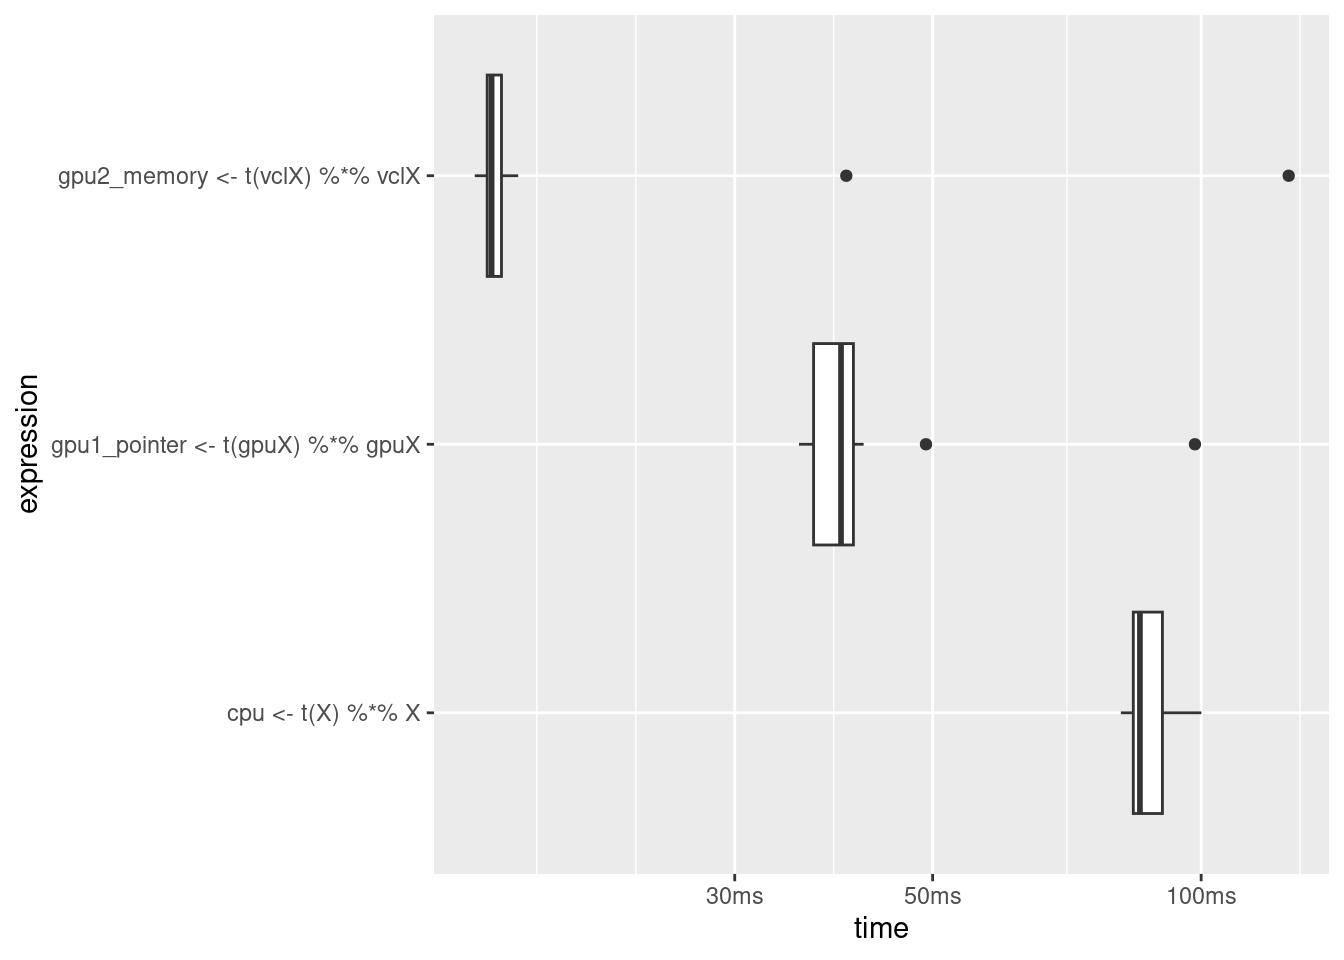
\includegraphics{bigdata_files/figure-latex/unnamed-chunk-59-1.pdf}

\hypertarget{vectorization}{%
\subsubsection{Vectorization}\label{vectorization}}

We can further improve the performance of this function by exploiting the fact that in R `everything is a vector' and that many of the basic R functions (such as math operators) are \emph{vectorized}. In simple terms, this means that an operation is implemented to directly work on vectors in such a way that it can take advantage of the similarity of each of the vector's elements. That is, R only has to figure out once how to apply a given function to a vector element in order to apply it to all elements of the vector. In a simple loop, R has to go through the same `preparatory' steps again and again in each iteration.

\begin{Shaded}
\begin{Highlighting}[]
\CommentTok{\# implementation with vectorization}
\NormalTok{sqrt\_vector\_fastest }\OtherTok{\textless{}{-}} 
     \ControlFlowTok{function}\NormalTok{(x) \{}
\NormalTok{               output }\OtherTok{\textless{}{-}}\NormalTok{  x}\SpecialCharTok{\^{}}\NormalTok{(}\DecValTok{1}\SpecialCharTok{/}\DecValTok{2}\NormalTok{)}
          \FunctionTok{return}\NormalTok{(output)}
\NormalTok{     \}}

\CommentTok{\# speed test}
\NormalTok{output\_fastest }\OtherTok{\textless{}{-}} 
     \FunctionTok{sapply}\NormalTok{(inputs, }
            \ControlFlowTok{function}\NormalTok{(x)\{ }\FunctionTok{system.time}\NormalTok{(}\FunctionTok{sqrt\_vector\_fastest}\NormalTok{(x))[}\StringTok{"elapsed"}\NormalTok{]}
\NormalTok{                 \}}
\NormalTok{            )}
\end{Highlighting}
\end{Shaded}

Let's have a look at whether this improves the function's performance further.

\begin{Shaded}
\begin{Highlighting}[]
\CommentTok{\# load packages}
\FunctionTok{library}\NormalTok{(ggplot2)}

\CommentTok{\# initiate data frame for plot}
\NormalTok{plotdata }\OtherTok{\textless{}{-}} \FunctionTok{data.frame}\NormalTok{(}\AttributeTok{time\_elapsed =} \FunctionTok{c}\NormalTok{(output\_faster, output\_fastest),}
                       \AttributeTok{input\_size =} \FunctionTok{c}\NormalTok{(input\_sizes, input\_sizes),}
                       \AttributeTok{Implementation=} \FunctionTok{c}\NormalTok{(}\FunctionTok{rep}\NormalTok{(}\StringTok{"sqrt\_vector\_faster"}\NormalTok{, }\FunctionTok{length}\NormalTok{(output\_faster)),}
                            \FunctionTok{rep}\NormalTok{(}\StringTok{"sqrt\_vector\_fastest"}\NormalTok{, }\FunctionTok{length}\NormalTok{(output\_fastest))))}

\CommentTok{\# plot}
\FunctionTok{ggplot}\NormalTok{(plotdata, }\FunctionTok{aes}\NormalTok{(}\AttributeTok{x=}\NormalTok{input\_size, }\AttributeTok{y=}\NormalTok{ time\_elapsed)) }\SpecialCharTok{+}
     \FunctionTok{geom\_point}\NormalTok{(}\FunctionTok{aes}\NormalTok{(}\AttributeTok{colour=}\NormalTok{Implementation)) }\SpecialCharTok{+}
     \FunctionTok{theme\_minimal}\NormalTok{(}\AttributeTok{base\_size =} \DecValTok{18}\NormalTok{) }\SpecialCharTok{+}
     \FunctionTok{ylab}\NormalTok{(}\StringTok{"Time elapsed (in seconds)"}\NormalTok{) }\SpecialCharTok{+}
     \FunctionTok{xlab}\NormalTok{(}\StringTok{"No. of elements processed"}\NormalTok{)}
\end{Highlighting}
\end{Shaded}

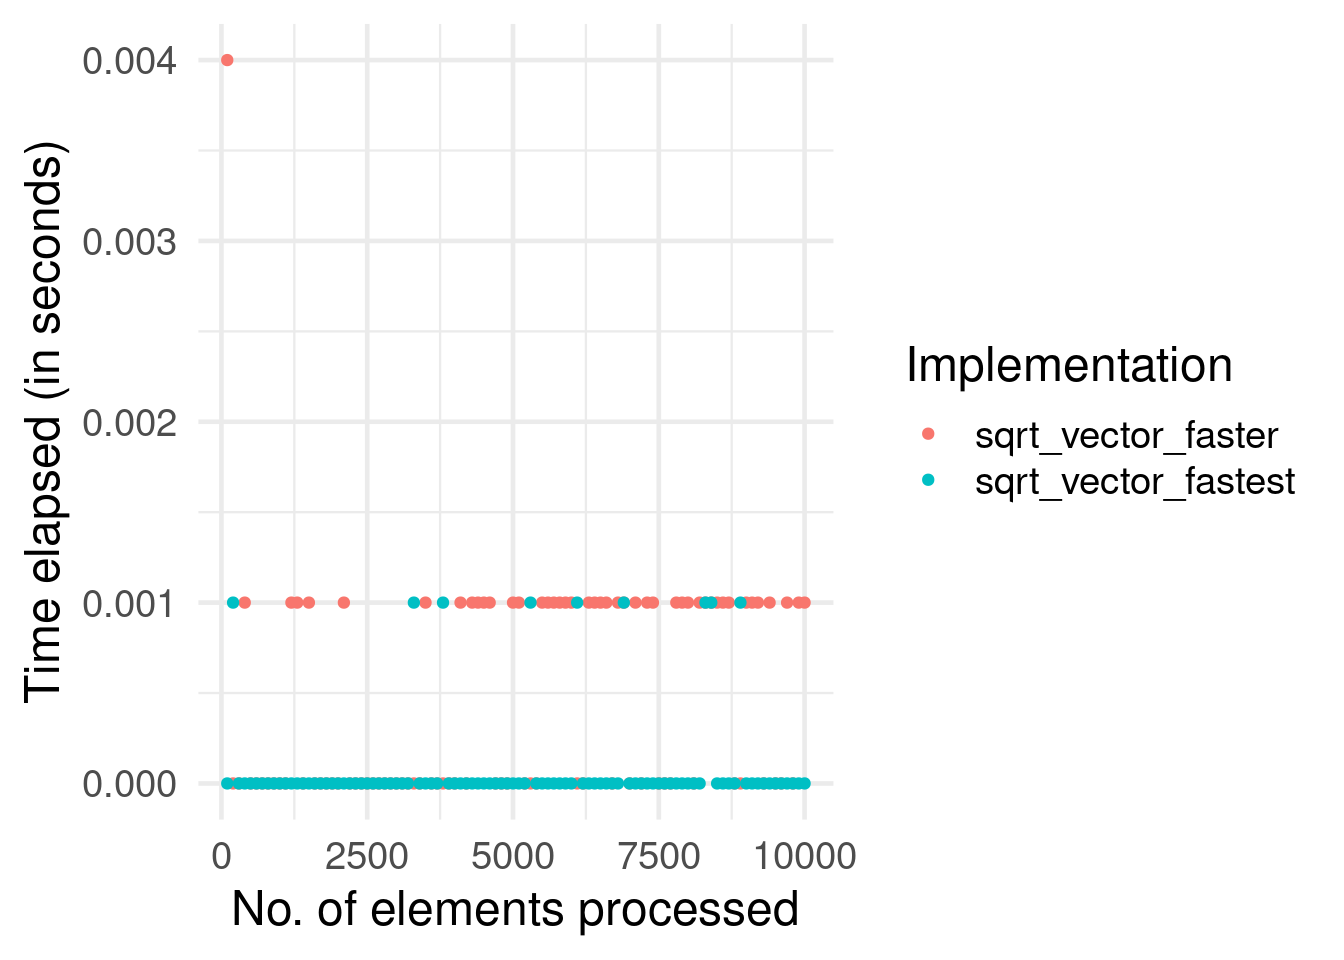
\includegraphics{bigdata_files/figure-latex/unnamed-chunk-61-1.pdf}

In the example above, we have simply exploited the fact that many of R's basic functions (such as math operators) are vectorized. If the program we want to implement cannot directly benefit from such a function, there are basically two ways to make use of vectorization (instead of loops written in R).

One approach is to use an \texttt{apply}-type function instead of loops. Probably most widely used is \texttt{lapply()}, a function that takes a vector (atomic or list) as input and applies a function \texttt{FUN} to each of its elements. It is a straightforward alternative to \texttt{for}-loops in many situations. The following example shows how we can get the same result by either writing a loop or using \texttt{lapply()}. The aim of the code example is to import the \href{https://archive.ics.uci.edu/ml/datasets/Health+News+in+Twitter}{Health News in Twitter Data Set} by \citet{karami_etal2017}. The raw data consists of several text files that need to be imported to R consecutively.

The text-files are located in \texttt{data/twitter\_texts/}. For either approach of importing all of these files, we first need a list of the paths to all of the files. We can get this with \texttt{list.files()}. Also, for either approach we will make use of the \texttt{fread}-function in the \texttt{data.table}-package.

\begin{Shaded}
\begin{Highlighting}[]
\CommentTok{\# load packages}
\FunctionTok{library}\NormalTok{(data.table)}

\CommentTok{\# get a list of all file{-}paths}
\NormalTok{textfiles }\OtherTok{\textless{}{-}} \FunctionTok{list.files}\NormalTok{(}\StringTok{"data/twitter\_texts"}\NormalTok{, }\AttributeTok{full.names =} \ConstantTok{TRUE}\NormalTok{)}
\end{Highlighting}
\end{Shaded}

Now we can read in all the text files with a \texttt{for}-loop as follows.

\begin{Shaded}
\begin{Highlighting}[]
\CommentTok{\# prepare loop}
\NormalTok{all\_texts }\OtherTok{\textless{}{-}} \FunctionTok{list}\NormalTok{()}
\NormalTok{n\_files }\OtherTok{\textless{}{-}} \FunctionTok{length}\NormalTok{(textfiles)}
\FunctionTok{length}\NormalTok{(all\_texts) }\OtherTok{\textless{}{-}}\NormalTok{ n\_files}
\CommentTok{\# read all files listed in textfiles}
\ControlFlowTok{for}\NormalTok{ (i }\ControlFlowTok{in} \DecValTok{1}\SpecialCharTok{:}\NormalTok{n\_files) \{}
\NormalTok{     all\_texts[[i]] }\OtherTok{\textless{}{-}} \FunctionTok{fread}\NormalTok{(textfiles[i])}
\NormalTok{\}}
\end{Highlighting}
\end{Shaded}

The imported files are now stored as \texttt{data.table}-objects in the list \texttt{all\_texts}. With the following line of code we combine all of them in one \texttt{data.table}.

\begin{Shaded}
\begin{Highlighting}[]
\CommentTok{\# combine all in one data.table}
\NormalTok{twitter\_text }\OtherTok{\textless{}{-}} \FunctionTok{rbindlist}\NormalTok{(all\_texts)}
\CommentTok{\# check result}
\FunctionTok{str}\NormalTok{(twitter\_text)}
\end{Highlighting}
\end{Shaded}

\begin{verbatim}
## Classes 'data.table' and 'data.frame':   42422 obs. of  3 variables:
##  $ V1:integer64 585978391360221184 585947808772960257 585947807816650752 585866060991078401 585794106170839041 585733482413891584 585733481608646657 585701601131765761 ... 
##  $ V2: chr  "Thu Apr 09 01:31:50 +0000 2015" "Wed Apr 08 23:30:18 +0000 2015" "Wed Apr 08 23:30:18 +0000 2015" "Wed Apr 08 18:05:28 +0000 2015" ...
##  $ V3: chr  "Breast cancer risk test devised http://bbc.in/1CimpJF" "GP workload harming care - BMA poll http://bbc.in/1ChTBRv" "Short people's 'heart risk greater' http://bbc.in/1ChTANp" "New approach against HIV 'promising' http://bbc.in/1E6jAjt" ...
##  - attr(*, ".internal.selfref")=<externalptr>
\end{verbatim}

Alternatively, we can make use of \texttt{lapply} as follows in order to achieve exactly the same.

\begin{Shaded}
\begin{Highlighting}[]
\CommentTok{\# prepare loop}
\NormalTok{all\_texts }\OtherTok{\textless{}{-}} \FunctionTok{lapply}\NormalTok{(textfiles, fread)}
\CommentTok{\# combine all in one data.table}
\NormalTok{twitter\_text }\OtherTok{\textless{}{-}} \FunctionTok{rbindlist}\NormalTok{(all\_texts)}
\CommentTok{\# check result}
\FunctionTok{str}\NormalTok{(twitter\_text)}
\end{Highlighting}
\end{Shaded}

\begin{verbatim}
## Classes 'data.table' and 'data.frame':   42422 obs. of  3 variables:
##  $ V1:integer64 585978391360221184 585947808772960257 585947807816650752 585866060991078401 585794106170839041 585733482413891584 585733481608646657 585701601131765761 ... 
##  $ V2: chr  "Thu Apr 09 01:31:50 +0000 2015" "Wed Apr 08 23:30:18 +0000 2015" "Wed Apr 08 23:30:18 +0000 2015" "Wed Apr 08 18:05:28 +0000 2015" ...
##  $ V3: chr  "Breast cancer risk test devised http://bbc.in/1CimpJF" "GP workload harming care - BMA poll http://bbc.in/1ChTBRv" "Short people's 'heart risk greater' http://bbc.in/1ChTANp" "New approach against HIV 'promising' http://bbc.in/1E6jAjt" ...
##  - attr(*, ".internal.selfref")=<externalptr>
\end{verbatim}

Finally, we can make use of \texttt{Vectorization()} in order to `vectorize' (as far as possible) our own import function (written for this example).

\begin{Shaded}
\begin{Highlighting}[]
\CommentTok{\# initiate the import function}
\NormalTok{import\_file }\OtherTok{\textless{}{-}} 
     \ControlFlowTok{function}\NormalTok{(x) \{}
\NormalTok{          parsed\_x }\OtherTok{\textless{}{-}} \FunctionTok{fread}\NormalTok{(x)}
          \FunctionTok{return}\NormalTok{(parsed\_x)}
\NormalTok{     \}}

\CommentTok{\# \textquotesingle{}vectorize\textquotesingle{} it}
\NormalTok{import\_files }\OtherTok{\textless{}{-}} \FunctionTok{Vectorize}\NormalTok{(import\_file, }\AttributeTok{SIMPLIFY =} \ConstantTok{FALSE}\NormalTok{)}

\CommentTok{\# Apply the vectorized function}
\NormalTok{all\_texts }\OtherTok{\textless{}{-}} \FunctionTok{import\_files}\NormalTok{(textfiles)}
\NormalTok{twitter\_text }\OtherTok{\textless{}{-}} \FunctionTok{rbindlist}\NormalTok{(all\_texts)}
\CommentTok{\# check the result}
\FunctionTok{str}\NormalTok{(twitter\_text)}
\end{Highlighting}
\end{Shaded}

\begin{verbatim}
## Classes 'data.table' and 'data.frame':   42422 obs. of  3 variables:
##  $ V1:integer64 585978391360221184 585947808772960257 585947807816650752 585866060991078401 585794106170839041 585733482413891584 585733481608646657 585701601131765761 ... 
##  $ V2: chr  "Thu Apr 09 01:31:50 +0000 2015" "Wed Apr 08 23:30:18 +0000 2015" "Wed Apr 08 23:30:18 +0000 2015" "Wed Apr 08 18:05:28 +0000 2015" ...
##  $ V3: chr  "Breast cancer risk test devised http://bbc.in/1CimpJF" "GP workload harming care - BMA poll http://bbc.in/1ChTBRv" "Short people's 'heart risk greater' http://bbc.in/1ChTANp" "New approach against HIV 'promising' http://bbc.in/1E6jAjt" ...
##  - attr(*, ".internal.selfref")=<externalptr>
\end{verbatim}

\hypertarget{r-beyond-r}{%
\subsection{R, beyond R}\label{r-beyond-r}}

So far, we have explored idiosyncrasies of R we should be aware of when writing programs to handle and analyze large data sets. While this has shown that R has many advantages for working with data, it also revealed some aspects of R that might result in low performance compared other programming languages. A simple generic explanation for this is that R is an \href{https://en.wikipedia.org/wiki/Interpreted_language}{interpreted language}, meaning that when we execute R code, it is processed (statement by statement) by an `interpreter' that translates the code into machine code (without the user giving any specific instructions). In contrast, when writing code in a `compiled language', we first have to explicitly compile the code and then run the compiled program. Running code that is already compiled is typically much faster than running R code that has to be interpreted before it can actually be processed by the CPU.

For advanced programmers, R offers various options to directly make use of compiled programs (for example, written in C, C++, or FORTRAN). In fact several of the core R functions installed with the basic R distribution are implemented in one of these lower-level programming languages and the R function we call simply interacts with these functions.

We can actually investigate this by looking at the source code of an R function. When simply typing the name of a function (such as our \texttt{import\_file()}) to the console, R is printing the function's source code to the console.

\begin{Shaded}
\begin{Highlighting}[]
\NormalTok{import\_file}
\end{Highlighting}
\end{Shaded}

\begin{verbatim}
## function(x) {
##           parsed_x <- fread(x)
##           return(parsed_x)
##      }
## <bytecode: 0x5623fbb40fc8>
\end{verbatim}

However, if we do the same for function \texttt{sum}, we don't see any actual source code.

\begin{Shaded}
\begin{Highlighting}[]
\NormalTok{sum}
\end{Highlighting}
\end{Shaded}

\begin{verbatim}
## function (..., na.rm = FALSE)  .Primitive("sum")
\end{verbatim}

Instead \texttt{.Primitive()} indicates that \texttt{sum()} is actually referring to an internal function (in this case implemented in C).

While the use of functions implemented in a lower-level language is a common technique to improve the speed of `R' functions, it is particularly prominent in the context of functions/packages made to deal with large amounts of data (such as the \texttt{data.table} package).

\hypertarget{big-data-cleaning-and-transformation}{%
\chapter{Big Data Cleaning and Transformation}\label{big-data-cleaning-and-transformation}}

Preceding the filtering/selection/aggregation of raw data, data cleaning and transformation typically have to be run on large parts of the overall dataset. In practice, the bottleneck is often a lack of RAM. In the following, we explore two strategies that broadly build on the idea of \emph{virtual memory} (using parts of the hard disk as RAM).

\hypertarget{out-of-memory-strategies}{%
\section{`Out-of-memory' strategies}\label{out-of-memory-strategies}}

Virtual memory is in simple words an approach to combining the RAM and mass storage components in order to cope with a lack of RAM. Modern operating systems come with a virtual memory manager that would automatically handle the swapping between RAM and the hard-disk, when running processes that use up too much RAM. However, a virtual memory manager is not specifically developed to perform this task in the context of data analysis. Several strategies have thus been developed to build on the basic idea of virtual memory in the context of data analysis tasks.

\begin{itemize}
\item
  \emph{Chunked data files on disk}: The data analytics software `partitions' the large dataset, maps, and stores the chunks of raw data on disk. What is actually `read' into RAM when importing the data file with this approach is the mapping to the partitions of the actual dataset (the data structure) and some metadata describing the dataset. In R, this approach is implemented in the \texttt{ff} package and several packages building on \texttt{ff}. In this approach, the usage of disk space and the linking between RAM and files on disk is very explicit (and well visible to the user).
\item
  \emph{Memory mapped files and shared memory}: The data analytics software uses segments of virtual memory for the dataset and allows different programs/processes to access it in the same memory segment. Thus, virtual memory is explicitly allocated for one or several specific data analytics tasks. In R, this approach is prominently implemented in the \texttt{bigmemory} package and several packages building on \texttt{bigmemory}.
\end{itemize}

\hypertarget{chunking-data-with-the-ff-package}{%
\subsection{\texorpdfstring{Chunking data with the \texttt{ff}-package}{Chunking data with the ff-package}}\label{chunking-data-with-the-ff-package}}

Before looking at the more detailed code examples in \citet{walkowiak_2016}, we investigate how the \texttt{ff} package (and the concept of chunked files) basically works. In order to do so, we first install and load the \texttt{ff} and \texttt{ffbase} packages, as well as the \texttt{pryr} package. We use the already known \texttt{flights.csv}-dataset as an example. When importing data via the \texttt{ff} package, we first have to set up a directory where \texttt{ff} can store the partitioned dataset (recall that this is explicitly/visibly done on disk). As in the code examples of the book, we call this new directory \texttt{ffdf} (after \texttt{ff}-data.frame).

\begin{Shaded}
\begin{Highlighting}[]
\CommentTok{\# SET UP {-}{-}{-}{-}{-}{-}{-}{-}{-}{-}{-}{-}{-}{-}}

\CommentTok{\# install.packages(c("ff", "ffbase"))}
\CommentTok{\# load packages}
\FunctionTok{library}\NormalTok{(ff)}
\FunctionTok{library}\NormalTok{(ffbase)}
\FunctionTok{library}\NormalTok{(pryr)}

\CommentTok{\# create directory for ff chunks, and assign directory to ff }
\FunctionTok{system}\NormalTok{(}\StringTok{"mkdir ffdf"}\NormalTok{)}
\FunctionTok{options}\NormalTok{(}\AttributeTok{fftempdir =} \StringTok{"ffdf"}\NormalTok{)}
\end{Highlighting}
\end{Shaded}

Now we can read in the data with \texttt{read.table.ffdf}. In order to better understand the underlying concept, we record the change in memory in the R environment with \texttt{mem\_change()}.

\begin{Shaded}
\begin{Highlighting}[]
\FunctionTok{mem\_change}\NormalTok{(}
\NormalTok{flights }\OtherTok{\textless{}{-}} 
     \FunctionTok{read.table.ffdf}\NormalTok{(}\AttributeTok{file=}\StringTok{"data/flights.csv"}\NormalTok{,}
                     \AttributeTok{sep=}\StringTok{","}\NormalTok{,}
                     \AttributeTok{VERBOSE=}\ConstantTok{TRUE}\NormalTok{,}
                     \AttributeTok{header=}\ConstantTok{TRUE}\NormalTok{,}
                     \AttributeTok{next.rows=}\DecValTok{100000}\NormalTok{,}
                     \AttributeTok{colClasses=}\ConstantTok{NA}\NormalTok{)}
\NormalTok{)}
\end{Highlighting}
\end{Shaded}

\begin{verbatim}
## read.table.ffdf 1..100000 (100000)  csv-read=0.341sec ffdf-write=0.037sec
## read.table.ffdf 100001..200000 (100000)  csv-read=0.343sec ffdf-write=0.025sec
## read.table.ffdf 200001..300000 (100000)  csv-read=0.354sec ffdf-write=0.024sec
## read.table.ffdf 300001..336776 (36776)  csv-read=0.135sec ffdf-write=0.015sec
##  csv-read=1.173sec  ffdf-write=0.101sec  TOTAL=1.274sec
\end{verbatim}

\begin{verbatim}
## -30.1 MB
\end{verbatim}

Note that there are two substantial differences to what we have previously seen when using \texttt{fread()}. It takes much longer to import a csv into the ffdf structure. However, the RAM allocated to it is much smaller. This is exactly what we would expect, keeping in mind what \texttt{read.table.ffdf()} does in comparison to what \texttt{fread()} does.

Now we can actually have a look at the data chunks created by \texttt{ff}, as well as how the structure of the dataset is represented in the \texttt{flights} object.

\begin{Shaded}
\begin{Highlighting}[]
\CommentTok{\# show the files in the directory keeping the chunks}
\FunctionTok{list.files}\NormalTok{(}\StringTok{"ffdf"}\NormalTok{)}
\end{Highlighting}
\end{Shaded}

\begin{verbatim}
##   [1] "clone75db307fa93.ff"  "clone75db47da7f7a.ff"
##   [3] "clone75db4bd01be5.ff" "clone75db50764070.ff"
##   [5] "clone8e35360e6853.ff" "clone8e3557fa7930.ff"
##   [7] "clone8e355e79fe83.ff" "clone8e3579525b87.ff"
##   [9] "clone9ff63cab7f09.ff" "clone9ff64610abb0.ff"
##  [11] "clone9ff65c23f55c.ff" "clone9ff67a994b7.ff" 
##  [13] "ff75db238f2277.ff"    "ff75db467c9ca9.ff"   
##  [15] "ff75db5b8705e6.ff"    "ff8e351f52edee.ff"   
##  [17] "ff8e357931e350.ff"    "ff8e3579acefd2.ff"   
##  [19] "ff9ff6166e92fc.ff"    "ff9ff6333e8cb9.ff"   
##  [21] "ff9ff67f69f9c8.ff"    "ffdf75db104a61b5.ff" 
##  [23] "ffdf75db12381c2.ff"   "ffdf75db12f4060b.ff" 
##  [25] "ffdf75db155ac869.ff"  "ffdf75db17569ab7.ff" 
##  [27] "ffdf75db19bd3c44.ff"  "ffdf75db1a31be36.ff" 
##  [29] "ffdf75db1acb53f1.ff"  "ffdf75db1afbc30.ff"  
##  [31] "ffdf75db1bdd3923.ff"  "ffdf75db1efba4e.ff"  
##  [33] "ffdf75db1efd5577.ff"  "ffdf75db1fad0746.ff" 
##  [35] "ffdf75db20bb1ef4.ff"  "ffdf75db20d27dcd.ff" 
##  [37] "ffdf75db275c430a.ff"  "ffdf75db27b0c953.ff" 
##  [39] "ffdf75db28d5b230.ff"  "ffdf75db29b096a2.ff" 
##  [41] "ffdf75db2a510673.ff"  "ffdf75db2a523ee8.ff" 
##  [43] "ffdf75db2b240bf8.ff"  "ffdf75db2b9129e1.ff" 
##  [45] "ffdf75db2db0aa48.ff"  "ffdf75db30419c13.ff" 
##  [47] "ffdf75db31f15844.ff"  "ffdf75db3314da06.ff" 
##  [49] "ffdf75db37721ddc.ff"  "ffdf75db4068263a.ff" 
##  [51] "ffdf75db436e625f.ff"  "ffdf75db463b8db5.ff" 
##  [53] "ffdf75db46599881.ff"  "ffdf75db473e9042.ff" 
##  [55] "ffdf75db48cee0dd.ff"  "ffdf75db4990d124.ff" 
##  [57] "ffdf75db4b74a57c.ff"  "ffdf75db50e1e5ae.ff" 
##  [59] "ffdf75db51ec6609.ff"  "ffdf75db53cb1709.ff" 
##  [61] "ffdf75db54e2b89.ff"   "ffdf75db54f4609d.ff" 
##  [63] "ffdf75db561e924f.ff"  "ffdf75db5a2309c4.ff" 
##  [65] "ffdf75db5b1ae970.ff"  "ffdf75db5d1285ce.ff" 
##  [67] "ffdf75db5de853dd.ff"  "ffdf75db5efcb02.ff"  
##  [69] "ffdf75db60d638f6.ff"  "ffdf75db641578be.ff" 
##  [71] "ffdf75db662baee6.ff"  "ffdf75db66a014e2.ff" 
##  [73] "ffdf75db672c164e.ff"  "ffdf75db67e14b3c.ff" 
##  [75] "ffdf75db6a4f2906.ff"  "ffdf75db6ac4f9af.ff" 
##  [77] "ffdf75db6b4c5127.ff"  "ffdf75db6be87b71.ff" 
##  [79] "ffdf75db6c31c71.ff"   "ffdf75db6dc7633b.ff" 
##  [81] "ffdf75db6e06dd86.ff"  "ffdf75db6e99304b.ff" 
##  [83] "ffdf75db725a257d.ff"  "ffdf75db727076ab.ff" 
##  [85] "ffdf75db72b0340e.ff"  "ffdf75db74ef3a8a.ff" 
##  [87] "ffdf75db76e92b9f.ff"  "ffdf75db77643f09.ff" 
##  [89] "ffdf75db78083020.ff"  "ffdf75db7a0eb09f.ff" 
##  [91] "ffdf75db7b03a8df.ff"  "ffdf75db7deeba85.ff" 
##  [93] "ffdf75db7ee7bfbb.ff"  "ffdf75db80afc77.ff"  
##  [95] "ffdf75db9f8f75f.ff"   "ffdf75dbae90994.ff"  
##  [97] "ffdf75dbafc362c.ff"   "ffdf75dbb273f69.ff"  
##  [99] "ffdf75dbd1cd10.ff"    "ffdf8e3514dfade1.ff" 
## [101] "ffdf8e3515fa8211.ff"  "ffdf8e3518d21571.ff" 
## [103] "ffdf8e351c061b0e.ff"  "ffdf8e351d03c750.ff" 
## [105] "ffdf8e351f24f13c.ff"  "ffdf8e35204f468.ff"  
## [107] "ffdf8e3520749287.ff"  "ffdf8e35213843be.ff" 
## [109] "ffdf8e352157e257.ff"  "ffdf8e35238a0f83.ff" 
## [111] "ffdf8e352390a28e.ff"  "ffdf8e3523efdb6a.ff" 
## [113] "ffdf8e35243f7204.ff"  "ffdf8e35266058d8.ff" 
## [115] "ffdf8e352719254a.ff"  "ffdf8e352ac66b45.ff" 
## [117] "ffdf8e352b16ccee.ff"  "ffdf8e352c9928d7.ff" 
## [119] "ffdf8e352ead5d77.ff"  "ffdf8e35328682a.ff"  
## [121] "ffdf8e3532e1e0bb.ff"  "ffdf8e35377dee1d.ff" 
## [123] "ffdf8e3537cbb5c8.ff"  "ffdf8e353803181e.ff" 
## [125] "ffdf8e3538a78b41.ff"  "ffdf8e353944cdf5.ff" 
## [127] "ffdf8e353969089.ff"   "ffdf8e3539cc5f85.ff" 
## [129] "ffdf8e353addce7a.ff"  "ffdf8e353be15cf0.ff" 
## [131] "ffdf8e353d328ef5.ff"  "ffdf8e353d8d734a.ff" 
## [133] "ffdf8e3540097a02.ff"  "ffdf8e3541eb9253.ff" 
## [135] "ffdf8e3545c5183f.ff"  "ffdf8e354614e0dc.ff" 
## [137] "ffdf8e3546234b48.ff"  "ffdf8e35481464cb.ff" 
## [139] "ffdf8e35489d7a69.ff"  "ffdf8e354b58974e.ff" 
## [141] "ffdf8e354bfb4ef3.ff"  "ffdf8e354c620628.ff" 
## [143] "ffdf8e354c765b75.ff"  "ffdf8e354d797e22.ff" 
## [145] "ffdf8e354ede9f1e.ff"  "ffdf8e354fc4b1cb.ff" 
## [147] "ffdf8e354fe5a135.ff"  "ffdf8e3556bbe7be.ff" 
## [149] "ffdf8e35585756f5.ff"  "ffdf8e355a913a9b.ff" 
## [151] "ffdf8e355b526101.ff"  "ffdf8e355db9a2c5.ff" 
## [153] "ffdf8e355dbc3aef.ff"  "ffdf8e355f80a38f.ff" 
## [155] "ffdf8e355fd1385b.ff"  "ffdf8e3560253dd.ff"  
## [157] "ffdf8e35618f7b7f.ff"  "ffdf8e356624a0da.ff" 
## [159] "ffdf8e3567b93c51.ff"  "ffdf8e356b555a53.ff" 
## [161] "ffdf8e356b86f764.ff"  "ffdf8e356d73161.ff"  
## [163] "ffdf8e356f8dfd2f.ff"  "ffdf8e3570932676.ff" 
## [165] "ffdf8e35763e2d39.ff"  "ffdf8e3577a6492c.ff" 
## [167] "ffdf8e357862a5f.ff"   "ffdf8e3579b7481c.ff" 
## [169] "ffdf8e357a7ffc73.ff"  "ffdf8e357b0c82.ff"   
## [171] "ffdf8e357d0c49e9.ff"  "ffdf8e357def0110.ff" 
## [173] "ffdf8e3592a6f2a.ff"   "ffdf8e359ff998c.ff"  
## [175] "ffdf8e35a97707d.ff"   "ffdf8e35bfade79.ff"  
## [177] "ffdf8e35fd54512.ff"   "ffdf9ff6110d9311.ff" 
## [179] "ffdf9ff61187c490.ff"  "ffdf9ff6152ac306.ff" 
## [181] "ffdf9ff61c2ecc81.ff"  "ffdf9ff62432108c.ff" 
## [183] "ffdf9ff624d6cbd8.ff"  "ffdf9ff62567feaf.ff" 
## [185] "ffdf9ff625f9e3d2.ff"  "ffdf9ff62618d903.ff" 
## [187] "ffdf9ff6296ad395.ff"  "ffdf9ff629a507d5.ff" 
## [189] "ffdf9ff629cbcef2.ff"  "ffdf9ff62c372317.ff" 
## [191] "ffdf9ff62cc39202.ff"  "ffdf9ff62d35fc65.ff" 
## [193] "ffdf9ff62d599839.ff"  "ffdf9ff633d492f0.ff" 
## [195] "ffdf9ff63495cbc8.ff"  "ffdf9ff634fd2ad2.ff" 
## [197] "ffdf9ff6395cd393.ff"  "ffdf9ff63e0bcda8.ff" 
## [199] "ffdf9ff63e64c093.ff"  "ffdf9ff64079d5a1.ff" 
## [201] "ffdf9ff640be3484.ff"  "ffdf9ff642384989.ff" 
## [203] "ffdf9ff642644cae.ff"  "ffdf9ff6434d2842.ff" 
## [205] "ffdf9ff643a34c.ff"    "ffdf9ff648526631.ff" 
## [207] "ffdf9ff64a0de165.ff"  "ffdf9ff64c2ac858.ff" 
## [209] "ffdf9ff64cfd0de8.ff"  "ffdf9ff64fcab41a.ff" 
## [211] "ffdf9ff64fe4a7f6.ff"  "ffdf9ff650563688.ff" 
## [213] "ffdf9ff650a0349b.ff"  "ffdf9ff65108664e.ff" 
## [215] "ffdf9ff651294af2.ff"  "ffdf9ff6547a60a4.ff" 
## [217] "ffdf9ff654e3306a.ff"  "ffdf9ff65569dd2e.ff" 
## [219] "ffdf9ff655ad807a.ff"  "ffdf9ff65659d736.ff" 
## [221] "ffdf9ff657887beb.ff"  "ffdf9ff65a35c247.ff" 
## [223] "ffdf9ff65bac7761.ff"  "ffdf9ff65ca9604e.ff" 
## [225] "ffdf9ff65e6fe4d9.ff"  "ffdf9ff66015dce1.ff" 
## [227] "ffdf9ff6602d6eaa.ff"  "ffdf9ff660fb5d.ff"   
## [229] "ffdf9ff663959724.ff"  "ffdf9ff664b123d2.ff" 
## [231] "ffdf9ff6654a181b.ff"  "ffdf9ff66550a179.ff" 
## [233] "ffdf9ff66657df92.ff"  "ffdf9ff666899228.ff" 
## [235] "ffdf9ff66752f40.ff"   "ffdf9ff6676ad90.ff"  
## [237] "ffdf9ff66fc2c457.ff"  "ffdf9ff66fd9a106.ff" 
## [239] "ffdf9ff67007c538.ff"  "ffdf9ff6713b01bb.ff" 
## [241] "ffdf9ff6736f35c7.ff"  "ffdf9ff67554004d.ff" 
## [243] "ffdf9ff6759640a4.ff"  "ffdf9ff6760573f.ff"  
## [245] "ffdf9ff676501a5a.ff"  "ffdf9ff67aad6e23.ff" 
## [247] "ffdf9ff67caa956.ff"   "ffdf9ff67e922a3e.ff" 
## [249] "ffdf9ff6848f539.ff"   "ffdf9ff6939322e.ff"  
## [251] "ffdf9ff6a8f88eb.ff"   "ffdf9ff6aa707f0.ff"  
## [253] "ffdf9ff6aefa2ff.ff"   "ffdf9ff6b6d3522.ff"  
## [255] "ffdf9ff6dbb3e0b.ff"   "ffdfb3f6135820f4.ff" 
## [257] "ffdfb3f6142c50de.ff"  "ffdfb3f61cc2e3dd.ff" 
## [259] "ffdfb3f61ec07a7d.ff"  "ffdfb3f61f425c93.ff" 
## [261] "ffdfb3f62296082d.ff"  "ffdfb3f624e08b.ff"   
## [263] "ffdfb3f628f0eaa8.ff"  "ffdfb3f6344b78fe.ff" 
## [265] "ffdfb3f6446ce386.ff"  "ffdfb3f64c83ea00.ff" 
## [267] "ffdfb3f65fb8171c.ff"  "ffdfb3f66c2a1d45.ff" 
## [269] "ffdfb3f6723850c1.ff"  "ffdfb3f674888c10.ff" 
## [271] "ffdfb3f67562615a.ff"  "ffdfb3f67d8ec341.ff" 
## [273] "ffdfb3f67db25a8e.ff"  "ffdfb3f68550586.ff"
\end{verbatim}

\begin{Shaded}
\begin{Highlighting}[]
\CommentTok{\# investigate the structure of the object created in the R environment}
\FunctionTok{str}\NormalTok{(flights)}
\end{Highlighting}
\end{Shaded}

\begin{verbatim}
## List of 3
##  $ virtual: 'data.frame':    19 obs. of  7 variables:
##  .. $ VirtualVmode     : chr  "integer" "integer" "integer" "integer" ...
##  .. $ AsIs             : logi  FALSE FALSE FALSE FALSE FALSE FALSE ...
##  .. $ VirtualIsMatrix  : logi  FALSE FALSE FALSE FALSE FALSE FALSE ...
##  .. $ PhysicalIsMatrix : logi  FALSE FALSE FALSE FALSE FALSE FALSE ...
##  .. $ PhysicalElementNo: int  1 2 3 4 5 6 7 8 9 10 ...
##  .. $ PhysicalFirstCol : int  1 1 1 1 1 1 1 1 1 1 ...
##  .. $ PhysicalLastCol  : int  1 1 1 1 1 1 1 1 1 1 ...
##  .. - attr(*, "Dim")= int [1:2] 336776 19
##  .. - attr(*, "Dimorder")= int [1:2] 1 2
##  $ physical: List of 19
##  .. $ year          : list()
##  ..  ..- attr(*, "physical")=Class 'ff_pointer' <externalptr> 
##  ..  .. ..- attr(*, "vmode")= chr "integer"
##  ..  .. ..- attr(*, "maxlength")= int 336776
##  ..  .. ..- attr(*, "pattern")= chr "ffdf"
##  ..  .. ..- attr(*, "filename")= chr "/home/umatter/Dropbox/Teaching/HSG/BigData/BigData/ffdf/ffdfb3f67d8ec341.ff"
##  ..  .. ..- attr(*, "pagesize")= int 65536
##  ..  .. ..- attr(*, "finalizer")= chr "close"
##  ..  .. ..- attr(*, "finonexit")= logi TRUE
##  ..  .. ..- attr(*, "readonly")= logi FALSE
##  ..  .. ..- attr(*, "caching")= chr "mmnoflush"
##  ..  ..- attr(*, "virtual")= list()
##  ..  .. ..- attr(*, "Length")= int 336776
##  ..  .. ..- attr(*, "Symmetric")= logi FALSE
##  ..  .. ..- attr(*, "class")= chr "virtual"
##  .. .. - attr(*, "class") =  chr [1:2] "ff_vector" "ff"
##  .. $ month         : list()
##  ..  ..- attr(*, "physical")=Class 'ff_pointer' <externalptr> 
##  ..  .. ..- attr(*, "vmode")= chr "integer"
##  ..  .. ..- attr(*, "maxlength")= int 336776
##  ..  .. ..- attr(*, "pattern")= chr "ffdf"
##  ..  .. ..- attr(*, "filename")= chr "/home/umatter/Dropbox/Teaching/HSG/BigData/BigData/ffdf/ffdfb3f6135820f4.ff"
##  ..  .. ..- attr(*, "pagesize")= int 65536
##  ..  .. ..- attr(*, "finalizer")= chr "close"
##  ..  .. ..- attr(*, "finonexit")= logi TRUE
##  ..  .. ..- attr(*, "readonly")= logi FALSE
##  ..  .. ..- attr(*, "caching")= chr "mmnoflush"
##  ..  ..- attr(*, "virtual")= list()
##  ..  .. ..- attr(*, "Length")= int 336776
##  ..  .. ..- attr(*, "Symmetric")= logi FALSE
##  ..  .. ..- attr(*, "class")= chr "virtual"
##  .. .. - attr(*, "class") =  chr [1:2] "ff_vector" "ff"
##  .. $ day           : list()
##  ..  ..- attr(*, "physical")=Class 'ff_pointer' <externalptr> 
##  ..  .. ..- attr(*, "vmode")= chr "integer"
##  ..  .. ..- attr(*, "maxlength")= int 336776
##  ..  .. ..- attr(*, "pattern")= chr "ffdf"
##  ..  .. ..- attr(*, "filename")= chr "/home/umatter/Dropbox/Teaching/HSG/BigData/BigData/ffdf/ffdfb3f62296082d.ff"
##  ..  .. ..- attr(*, "pagesize")= int 65536
##  ..  .. ..- attr(*, "finalizer")= chr "close"
##  ..  .. ..- attr(*, "finonexit")= logi TRUE
##  ..  .. ..- attr(*, "readonly")= logi FALSE
##  ..  .. ..- attr(*, "caching")= chr "mmnoflush"
##  ..  ..- attr(*, "virtual")= list()
##  ..  .. ..- attr(*, "Length")= int 336776
##  ..  .. ..- attr(*, "Symmetric")= logi FALSE
##  ..  .. ..- attr(*, "class")= chr "virtual"
##  .. .. - attr(*, "class") =  chr [1:2] "ff_vector" "ff"
##  .. $ dep_time      : list()
##  ..  ..- attr(*, "physical")=Class 'ff_pointer' <externalptr> 
##  ..  .. ..- attr(*, "vmode")= chr "integer"
##  ..  .. ..- attr(*, "maxlength")= int 336776
##  ..  .. ..- attr(*, "pattern")= chr "ffdf"
##  ..  .. ..- attr(*, "filename")= chr "/home/umatter/Dropbox/Teaching/HSG/BigData/BigData/ffdf/ffdfb3f674888c10.ff"
##  ..  .. ..- attr(*, "pagesize")= int 65536
##  ..  .. ..- attr(*, "finalizer")= chr "close"
##  ..  .. ..- attr(*, "finonexit")= logi TRUE
##  ..  .. ..- attr(*, "readonly")= logi FALSE
##  ..  .. ..- attr(*, "caching")= chr "mmnoflush"
##  ..  ..- attr(*, "virtual")= list()
##  ..  .. ..- attr(*, "Length")= int 336776
##  ..  .. ..- attr(*, "Symmetric")= logi FALSE
##  ..  .. ..- attr(*, "class")= chr "virtual"
##  .. .. - attr(*, "class") =  chr [1:2] "ff_vector" "ff"
##  .. $ sched_dep_time: list()
##  ..  ..- attr(*, "physical")=Class 'ff_pointer' <externalptr> 
##  ..  .. ..- attr(*, "vmode")= chr "integer"
##  ..  .. ..- attr(*, "maxlength")= int 336776
##  ..  .. ..- attr(*, "pattern")= chr "ffdf"
##  ..  .. ..- attr(*, "filename")= chr "/home/umatter/Dropbox/Teaching/HSG/BigData/BigData/ffdf/ffdfb3f67db25a8e.ff"
##  ..  .. ..- attr(*, "pagesize")= int 65536
##  ..  .. ..- attr(*, "finalizer")= chr "close"
##  ..  .. ..- attr(*, "finonexit")= logi TRUE
##  ..  .. ..- attr(*, "readonly")= logi FALSE
##  ..  .. ..- attr(*, "caching")= chr "mmnoflush"
##  ..  ..- attr(*, "virtual")= list()
##  ..  .. ..- attr(*, "Length")= int 336776
##  ..  .. ..- attr(*, "Symmetric")= logi FALSE
##  ..  .. ..- attr(*, "class")= chr "virtual"
##  .. .. - attr(*, "class") =  chr [1:2] "ff_vector" "ff"
##  .. $ dep_delay     : list()
##  ..  ..- attr(*, "physical")=Class 'ff_pointer' <externalptr> 
##  ..  .. ..- attr(*, "vmode")= chr "integer"
##  ..  .. ..- attr(*, "maxlength")= int 336776
##  ..  .. ..- attr(*, "pattern")= chr "ffdf"
##  ..  .. ..- attr(*, "filename")= chr "/home/umatter/Dropbox/Teaching/HSG/BigData/BigData/ffdf/ffdfb3f624e08b.ff"
##  ..  .. ..- attr(*, "pagesize")= int 65536
##  ..  .. ..- attr(*, "finalizer")= chr "close"
##  ..  .. ..- attr(*, "finonexit")= logi TRUE
##  ..  .. ..- attr(*, "readonly")= logi FALSE
##  ..  .. ..- attr(*, "caching")= chr "mmnoflush"
##  ..  ..- attr(*, "virtual")= list()
##  ..  .. ..- attr(*, "Length")= int 336776
##  ..  .. ..- attr(*, "Symmetric")= logi FALSE
##  ..  .. ..- attr(*, "class")= chr "virtual"
##  .. .. - attr(*, "class") =  chr [1:2] "ff_vector" "ff"
##  .. $ arr_time      : list()
##  ..  ..- attr(*, "physical")=Class 'ff_pointer' <externalptr> 
##  ..  .. ..- attr(*, "vmode")= chr "integer"
##  ..  .. ..- attr(*, "maxlength")= int 336776
##  ..  .. ..- attr(*, "pattern")= chr "ffdf"
##  ..  .. ..- attr(*, "filename")= chr "/home/umatter/Dropbox/Teaching/HSG/BigData/BigData/ffdf/ffdfb3f67562615a.ff"
##  ..  .. ..- attr(*, "pagesize")= int 65536
##  ..  .. ..- attr(*, "finalizer")= chr "close"
##  ..  .. ..- attr(*, "finonexit")= logi TRUE
##  ..  .. ..- attr(*, "readonly")= logi FALSE
##  ..  .. ..- attr(*, "caching")= chr "mmnoflush"
##  ..  ..- attr(*, "virtual")= list()
##  ..  .. ..- attr(*, "Length")= int 336776
##  ..  .. ..- attr(*, "Symmetric")= logi FALSE
##  ..  .. ..- attr(*, "class")= chr "virtual"
##  .. .. - attr(*, "class") =  chr [1:2] "ff_vector" "ff"
##  .. $ sched_arr_time: list()
##  ..  ..- attr(*, "physical")=Class 'ff_pointer' <externalptr> 
##  ..  .. ..- attr(*, "vmode")= chr "integer"
##  ..  .. ..- attr(*, "maxlength")= int 336776
##  ..  .. ..- attr(*, "pattern")= chr "ffdf"
##  ..  .. ..- attr(*, "filename")= chr "/home/umatter/Dropbox/Teaching/HSG/BigData/BigData/ffdf/ffdfb3f61f425c93.ff"
##  ..  .. ..- attr(*, "pagesize")= int 65536
##  ..  .. ..- attr(*, "finalizer")= chr "close"
##  ..  .. ..- attr(*, "finonexit")= logi TRUE
##  ..  .. ..- attr(*, "readonly")= logi FALSE
##  ..  .. ..- attr(*, "caching")= chr "mmnoflush"
##  ..  ..- attr(*, "virtual")= list()
##  ..  .. ..- attr(*, "Length")= int 336776
##  ..  .. ..- attr(*, "Symmetric")= logi FALSE
##  ..  .. ..- attr(*, "class")= chr "virtual"
##  .. .. - attr(*, "class") =  chr [1:2] "ff_vector" "ff"
##  .. $ arr_delay     : list()
##  ..  ..- attr(*, "physical")=Class 'ff_pointer' <externalptr> 
##  ..  .. ..- attr(*, "vmode")= chr "integer"
##  ..  .. ..- attr(*, "maxlength")= int 336776
##  ..  .. ..- attr(*, "pattern")= chr "ffdf"
##  ..  .. ..- attr(*, "filename")= chr "/home/umatter/Dropbox/Teaching/HSG/BigData/BigData/ffdf/ffdfb3f6723850c1.ff"
##  ..  .. ..- attr(*, "pagesize")= int 65536
##  ..  .. ..- attr(*, "finalizer")= chr "close"
##  ..  .. ..- attr(*, "finonexit")= logi TRUE
##  ..  .. ..- attr(*, "readonly")= logi FALSE
##  ..  .. ..- attr(*, "caching")= chr "mmnoflush"
##  ..  ..- attr(*, "virtual")= list()
##  ..  .. ..- attr(*, "Length")= int 336776
##  ..  .. ..- attr(*, "Symmetric")= logi FALSE
##  ..  .. ..- attr(*, "class")= chr "virtual"
##  .. .. - attr(*, "class") =  chr [1:2] "ff_vector" "ff"
##  .. $ carrier       : list()
##  ..  ..- attr(*, "physical")=Class 'ff_pointer' <externalptr> 
##  ..  .. ..- attr(*, "vmode")= chr "integer"
##  ..  .. ..- attr(*, "maxlength")= int 336776
##  ..  .. ..- attr(*, "pattern")= chr "ffdf"
##  ..  .. ..- attr(*, "filename")= chr "/home/umatter/Dropbox/Teaching/HSG/BigData/BigData/ffdf/ffdfb3f65fb8171c.ff"
##  ..  .. ..- attr(*, "pagesize")= int 65536
##  ..  .. ..- attr(*, "finalizer")= chr "close"
##  ..  .. ..- attr(*, "finonexit")= logi TRUE
##  ..  .. ..- attr(*, "readonly")= logi FALSE
##  ..  .. ..- attr(*, "caching")= chr "mmnoflush"
##  ..  ..- attr(*, "virtual")= list()
##  ..  .. ..- attr(*, "Length")= int 336776
##  ..  .. ..- attr(*, "Symmetric")= logi FALSE
##  ..  .. ..- attr(*, "Levels")= chr [1:16] "9E" "AA" "AS" "B6" ...
##  ..  .. ..- attr(*, "ramclass")= chr "factor"
##  ..  .. ..- attr(*, "class")= chr "virtual"
##  .. .. - attr(*, "class") =  chr [1:2] "ff_vector" "ff"
##  .. $ flight        : list()
##  ..  ..- attr(*, "physical")=Class 'ff_pointer' <externalptr> 
##  ..  .. ..- attr(*, "vmode")= chr "integer"
##  ..  .. ..- attr(*, "maxlength")= int 336776
##  ..  .. ..- attr(*, "pattern")= chr "ffdf"
##  ..  .. ..- attr(*, "filename")= chr "/home/umatter/Dropbox/Teaching/HSG/BigData/BigData/ffdf/ffdfb3f61ec07a7d.ff"
##  ..  .. ..- attr(*, "pagesize")= int 65536
##  ..  .. ..- attr(*, "finalizer")= chr "close"
##  ..  .. ..- attr(*, "finonexit")= logi TRUE
##  ..  .. ..- attr(*, "readonly")= logi FALSE
##  ..  .. ..- attr(*, "caching")= chr "mmnoflush"
##  ..  ..- attr(*, "virtual")= list()
##  ..  .. ..- attr(*, "Length")= int 336776
##  ..  .. ..- attr(*, "Symmetric")= logi FALSE
##  ..  .. ..- attr(*, "class")= chr "virtual"
##  .. .. - attr(*, "class") =  chr [1:2] "ff_vector" "ff"
##  .. $ tailnum       : list()
##  ..  ..- attr(*, "physical")=Class 'ff_pointer' <externalptr> 
##  ..  .. ..- attr(*, "vmode")= chr "integer"
##  ..  .. ..- attr(*, "maxlength")= int 336776
##  ..  .. ..- attr(*, "pattern")= chr "ffdf"
##  ..  .. ..- attr(*, "filename")= chr "/home/umatter/Dropbox/Teaching/HSG/BigData/BigData/ffdf/ffdfb3f6344b78fe.ff"
##  ..  .. ..- attr(*, "pagesize")= int 65536
##  ..  .. ..- attr(*, "finalizer")= chr "close"
##  ..  .. ..- attr(*, "finonexit")= logi TRUE
##  ..  .. ..- attr(*, "readonly")= logi FALSE
##  ..  .. ..- attr(*, "caching")= chr "mmnoflush"
##  ..  ..- attr(*, "virtual")= list()
##  ..  .. ..- attr(*, "Length")= int 336776
##  ..  .. ..- attr(*, "Symmetric")= logi FALSE
##  ..  .. ..- attr(*, "Levels")= chr [1:4044] "" "N0EGMQ" "N10156" "N102UW" ...
##  ..  .. ..- attr(*, "ramclass")= chr "factor"
##  ..  .. ..- attr(*, "class")= chr "virtual"
##  .. .. - attr(*, "class") =  chr [1:2] "ff_vector" "ff"
##  .. $ origin        : list()
##  ..  ..- attr(*, "physical")=Class 'ff_pointer' <externalptr> 
##  ..  .. ..- attr(*, "vmode")= chr "integer"
##  ..  .. ..- attr(*, "maxlength")= int 336776
##  ..  .. ..- attr(*, "pattern")= chr "ffdf"
##  ..  .. ..- attr(*, "filename")= chr "/home/umatter/Dropbox/Teaching/HSG/BigData/BigData/ffdf/ffdfb3f68550586.ff"
##  ..  .. ..- attr(*, "pagesize")= int 65536
##  ..  .. ..- attr(*, "finalizer")= chr "close"
##  ..  .. ..- attr(*, "finonexit")= logi TRUE
##  ..  .. ..- attr(*, "readonly")= logi FALSE
##  ..  .. ..- attr(*, "caching")= chr "mmnoflush"
##  ..  ..- attr(*, "virtual")= list()
##  ..  .. ..- attr(*, "Length")= int 336776
##  ..  .. ..- attr(*, "Symmetric")= logi FALSE
##  ..  .. ..- attr(*, "Levels")= chr [1:3] "EWR" "JFK" "LGA"
##  ..  .. ..- attr(*, "ramclass")= chr "factor"
##  ..  .. ..- attr(*, "class")= chr "virtual"
##  .. .. - attr(*, "class") =  chr [1:2] "ff_vector" "ff"
##  .. $ dest          : list()
##  ..  ..- attr(*, "physical")=Class 'ff_pointer' <externalptr> 
##  ..  .. ..- attr(*, "vmode")= chr "integer"
##  ..  .. ..- attr(*, "maxlength")= int 336776
##  ..  .. ..- attr(*, "pattern")= chr "ffdf"
##  ..  .. ..- attr(*, "filename")= chr "/home/umatter/Dropbox/Teaching/HSG/BigData/BigData/ffdf/ffdfb3f628f0eaa8.ff"
##  ..  .. ..- attr(*, "pagesize")= int 65536
##  ..  .. ..- attr(*, "finalizer")= chr "close"
##  ..  .. ..- attr(*, "finonexit")= logi TRUE
##  ..  .. ..- attr(*, "readonly")= logi FALSE
##  ..  .. ..- attr(*, "caching")= chr "mmnoflush"
##  ..  ..- attr(*, "virtual")= list()
##  ..  .. ..- attr(*, "Length")= int 336776
##  ..  .. ..- attr(*, "Symmetric")= logi FALSE
##  ..  .. ..- attr(*, "Levels")= chr [1:105] "ABQ" "ACK" "ALB" "ATL" ...
##  ..  .. ..- attr(*, "ramclass")= chr "factor"
##  ..  .. ..- attr(*, "class")= chr "virtual"
##  .. .. - attr(*, "class") =  chr [1:2] "ff_vector" "ff"
##  .. $ air_time      : list()
##  ..  ..- attr(*, "physical")=Class 'ff_pointer' <externalptr> 
##  ..  .. ..- attr(*, "vmode")= chr "integer"
##  ..  .. ..- attr(*, "maxlength")= int 336776
##  ..  .. ..- attr(*, "pattern")= chr "ffdf"
##  ..  .. ..- attr(*, "filename")= chr "/home/umatter/Dropbox/Teaching/HSG/BigData/BigData/ffdf/ffdfb3f61cc2e3dd.ff"
##  ..  .. ..- attr(*, "pagesize")= int 65536
##  ..  .. ..- attr(*, "finalizer")= chr "close"
##  ..  .. ..- attr(*, "finonexit")= logi TRUE
##  ..  .. ..- attr(*, "readonly")= logi FALSE
##  ..  .. ..- attr(*, "caching")= chr "mmnoflush"
##  ..  ..- attr(*, "virtual")= list()
##  ..  .. ..- attr(*, "Length")= int 336776
##  ..  .. ..- attr(*, "Symmetric")= logi FALSE
##  ..  .. ..- attr(*, "class")= chr "virtual"
##  .. .. - attr(*, "class") =  chr [1:2] "ff_vector" "ff"
##  .. $ distance      : list()
##  ..  ..- attr(*, "physical")=Class 'ff_pointer' <externalptr> 
##  ..  .. ..- attr(*, "vmode")= chr "integer"
##  ..  .. ..- attr(*, "maxlength")= int 336776
##  ..  .. ..- attr(*, "pattern")= chr "ffdf"
##  ..  .. ..- attr(*, "filename")= chr "/home/umatter/Dropbox/Teaching/HSG/BigData/BigData/ffdf/ffdfb3f64c83ea00.ff"
##  ..  .. ..- attr(*, "pagesize")= int 65536
##  ..  .. ..- attr(*, "finalizer")= chr "close"
##  ..  .. ..- attr(*, "finonexit")= logi TRUE
##  ..  .. ..- attr(*, "readonly")= logi FALSE
##  ..  .. ..- attr(*, "caching")= chr "mmnoflush"
##  ..  ..- attr(*, "virtual")= list()
##  ..  .. ..- attr(*, "Length")= int 336776
##  ..  .. ..- attr(*, "Symmetric")= logi FALSE
##  ..  .. ..- attr(*, "class")= chr "virtual"
##  .. .. - attr(*, "class") =  chr [1:2] "ff_vector" "ff"
##  .. $ hour          : list()
##  ..  ..- attr(*, "physical")=Class 'ff_pointer' <externalptr> 
##  ..  .. ..- attr(*, "vmode")= chr "integer"
##  ..  .. ..- attr(*, "maxlength")= int 336776
##  ..  .. ..- attr(*, "pattern")= chr "ffdf"
##  ..  .. ..- attr(*, "filename")= chr "/home/umatter/Dropbox/Teaching/HSG/BigData/BigData/ffdf/ffdfb3f6142c50de.ff"
##  ..  .. ..- attr(*, "pagesize")= int 65536
##  ..  .. ..- attr(*, "finalizer")= chr "close"
##  ..  .. ..- attr(*, "finonexit")= logi TRUE
##  ..  .. ..- attr(*, "readonly")= logi FALSE
##  ..  .. ..- attr(*, "caching")= chr "mmnoflush"
##  ..  ..- attr(*, "virtual")= list()
##  ..  .. ..- attr(*, "Length")= int 336776
##  ..  .. ..- attr(*, "Symmetric")= logi FALSE
##  ..  .. ..- attr(*, "class")= chr "virtual"
##  .. .. - attr(*, "class") =  chr [1:2] "ff_vector" "ff"
##  .. $ minute        : list()
##  ..  ..- attr(*, "physical")=Class 'ff_pointer' <externalptr> 
##  ..  .. ..- attr(*, "vmode")= chr "integer"
##  ..  .. ..- attr(*, "maxlength")= int 336776
##  ..  .. ..- attr(*, "pattern")= chr "ffdf"
##  ..  .. ..- attr(*, "filename")= chr "/home/umatter/Dropbox/Teaching/HSG/BigData/BigData/ffdf/ffdfb3f6446ce386.ff"
##  ..  .. ..- attr(*, "pagesize")= int 65536
##  ..  .. ..- attr(*, "finalizer")= chr "close"
##  ..  .. ..- attr(*, "finonexit")= logi TRUE
##  ..  .. ..- attr(*, "readonly")= logi FALSE
##  ..  .. ..- attr(*, "caching")= chr "mmnoflush"
##  ..  ..- attr(*, "virtual")= list()
##  ..  .. ..- attr(*, "Length")= int 336776
##  ..  .. ..- attr(*, "Symmetric")= logi FALSE
##  ..  .. ..- attr(*, "class")= chr "virtual"
##  .. .. - attr(*, "class") =  chr [1:2] "ff_vector" "ff"
##  .. $ time_hour     : list()
##  ..  ..- attr(*, "physical")=Class 'ff_pointer' <externalptr> 
##  ..  .. ..- attr(*, "vmode")= chr "integer"
##  ..  .. ..- attr(*, "maxlength")= int 336776
##  ..  .. ..- attr(*, "pattern")= chr "ffdf"
##  ..  .. ..- attr(*, "filename")= chr "/home/umatter/Dropbox/Teaching/HSG/BigData/BigData/ffdf/ffdfb3f66c2a1d45.ff"
##  ..  .. ..- attr(*, "pagesize")= int 65536
##  ..  .. ..- attr(*, "finalizer")= chr "close"
##  ..  .. ..- attr(*, "finonexit")= logi TRUE
##  ..  .. ..- attr(*, "readonly")= logi FALSE
##  ..  .. ..- attr(*, "caching")= chr "mmnoflush"
##  ..  ..- attr(*, "virtual")= list()
##  ..  .. ..- attr(*, "Length")= int 336776
##  ..  .. ..- attr(*, "Symmetric")= logi FALSE
##  ..  .. ..- attr(*, "Levels")= chr [1:6936] "2013-01-01T10:00:00Z" "2013-01-01T11:00:00Z" "2013-01-01T12:00:00Z" "2013-01-01T13:00:00Z" ...
##  ..  .. ..- attr(*, "ramclass")= chr "factor"
##  ..  .. ..- attr(*, "class")= chr "virtual"
##  .. .. - attr(*, "class") =  chr [1:2] "ff_vector" "ff"
##  $ row.names:  NULL
## - attributes: List of 2
##  .. $ names: chr [1:3] "virtual" "physical" "row.names"
##  .. $ class: chr "ffdf"
\end{verbatim}

\hypertarget{memory-mapping-with-bigmemory}{%
\subsection{\texorpdfstring{Memory mapping with \texttt{bigmemory}}{Memory mapping with bigmemory}}\label{memory-mapping-with-bigmemory}}

The \texttt{bigmemory}-package handles data in matrices, and therefore only accepts variables in the same data type. Before importing data via the \texttt{bigmemory}-package, we thus have to ensure that all variables in the raw data can be imported in a common type. This example follows the example of the package authors given \href{https://cran.r-project.org/web/packages/bigmemory/vignettes/Overview.pdf}{here}.\footnote{We only use a fraction of the data used in the package vignette example, the full raw data used there can be downloaded \href{http://stat-computing.org/dataexpo/2009/the-data.html}{here}.}

\begin{Shaded}
\begin{Highlighting}[]
\CommentTok{\# SET UP {-}{-}{-}{-}{-}{-}{-}{-}{-}{-}{-}{-}{-}{-}{-}{-}}

\CommentTok{\# load packages}
\FunctionTok{library}\NormalTok{(bigmemory)}
\FunctionTok{library}\NormalTok{(biganalytics)}

\CommentTok{\# import the data}
\NormalTok{flights }\OtherTok{\textless{}{-}} \FunctionTok{read.big.matrix}\NormalTok{(}\StringTok{"data/flights.csv"}\NormalTok{,}
                     \AttributeTok{type=}\StringTok{"integer"}\NormalTok{,}
                     \AttributeTok{header=}\ConstantTok{TRUE}\NormalTok{,}
                     \AttributeTok{backingfile=}\StringTok{"flights.bin"}\NormalTok{,}
                     \AttributeTok{descriptorfile=}\StringTok{"flights.desc"}\NormalTok{)}
\end{Highlighting}
\end{Shaded}

Note that, similar to the \texttt{ff}-example, \texttt{read.big.matrix()} initiates a local file-backing \texttt{flights.bin} on disk which is linked to the \texttt{flights}-object in RAM. From looking at the imported file, we see that various variable values have been discarded. This is due to the fact that we have forced all variables to be of type \texttt{"integer"} when importing the dataset.

\begin{Shaded}
\begin{Highlighting}[]
\FunctionTok{summary}\NormalTok{(flights)}
\end{Highlighting}
\end{Shaded}

\begin{verbatim}
##                       min        max       mean
## year             2013.000   2013.000   2013.000
## month               1.000     12.000      6.549
## day                 1.000     31.000     15.711
## dep_time            1.000   2400.000   1349.110
## sched_dep_time    106.000   2359.000   1344.255
## dep_delay         -43.000   1301.000     12.639
## arr_time            1.000   2400.000   1502.055
## sched_arr_time      1.000   2359.000   1536.380
## arr_delay         -86.000   1272.000      6.895
## carrier             9.000      9.000      9.000
## flight              1.000   8500.000   1971.924
## tailnum                                        
## origin                                         
## dest                                           
## air_time           20.000    695.000    150.686
## distance           17.000   4983.000   1039.913
## hour                1.000     23.000     13.180
## minute              0.000     59.000     26.230
## time_hour        2013.000   2014.000   2013.000
##                       NAs
## year                0.000
## month               0.000
## day                 0.000
## dep_time         8255.000
## sched_dep_time      0.000
## dep_delay        8255.000
## arr_time         8713.000
## sched_arr_time      0.000
## arr_delay        9430.000
## carrier        318316.000
## flight              0.000
## tailnum        336776.000
## origin         336776.000
## dest           336776.000
## air_time         9430.000
## distance            0.000
## hour                0.000
## minute              0.000
## time_hour           0.000
\end{verbatim}

\hypertarget{typical-cleaning-tasks}{%
\section{Typical cleaning tasks}\label{typical-cleaning-tasks}}

\begin{itemize}
\tightlist
\item
  Normalize/standardize.
\item
  Code additional variables (indicators, strings to categorical, etc.).
\item
  Remove, add covariates.
\item
  Merge data sets.
\item
  Set data types.
\end{itemize}

\begin{enumerate}
\def\labelenumi{\arabic{enumi}.}
\tightlist
\item
  Import raw data.
\item
  Clean/transform.
\item
  Store for analysis.

  \begin{itemize}
  \tightlist
  \item
    Write to file.
  \item
    Write to database.
  \end{itemize}
\end{enumerate}

\begin{itemize}
\tightlist
\item
  RAM:

  \begin{itemize}
  \tightlist
  \item
    Raw data does not fit into memory.
  \item
    Transformations enlarge RAM allocation (copying).
  \end{itemize}
\item
  Mass Storage: Reading/Writing
\item
  CPU: Parsing (data types)
\end{itemize}

\hypertarget{data-preparation-with-ff}{%
\subsection{\texorpdfstring{Data Preparation with \texttt{ff}}{Data Preparation with ff}}\label{data-preparation-with-ff}}

\hypertarget{set-up}{%
\subsubsection{Set up}\label{set-up}}

The following examples are based on \citet{walkowiak_2016}, Chapter 3. You can download the original datasets used in these examples from \href{https://github.com/PacktPublishing/Big-Data-Analytics-with-R/tree/master/Chapter\%203}{the book's GitHub repository}. The set up for our analysis script involves the loading of the \texttt{ff} and \texttt{ffbase} packages, the intitiation of fix variables to hold the paths to the data sets, as well as the creation and assignment of a new local directory \texttt{ffdf} in which the binary flat files-partitioned chunks of the original datasets will be stored.

\begin{Shaded}
\begin{Highlighting}[]
\DocumentationTok{\#\# SET UP {-}{-}{-}{-}{-}{-}{-}{-}{-}{-}{-}{-}{-}{-}{-}{-}{-}{-}{-}{-}{-}{-}{-}{-}}

\CommentTok{\# create and set directory for ff files}
\FunctionTok{system}\NormalTok{(}\StringTok{"mkdir ffdf"}\NormalTok{)}
\FunctionTok{options}\NormalTok{(}\AttributeTok{fftempdir =} \StringTok{"ffdf"}\NormalTok{)}

\CommentTok{\# load packages}
\FunctionTok{library}\NormalTok{(ff)}
\FunctionTok{library}\NormalTok{(ffbase)}
\FunctionTok{library}\NormalTok{(pryr)}

\CommentTok{\# fix vars}
\NormalTok{FLIGHTS\_DATA }\OtherTok{\textless{}{-}} \StringTok{"data/flights\_sep\_oct15.txt"}
\NormalTok{AIRLINES\_DATA }\OtherTok{\textless{}{-}} \StringTok{"data/airline\_id.csv"}
\end{Highlighting}
\end{Shaded}

\hypertarget{data-import}{%
\subsubsection{Data import}\label{data-import}}

In a first step we read (or `upload') the data into R. This step involves the creation of the binary chunked files as well as the mapping of these files and the metadata. In comparison to the traditional \texttt{read.csv} approach, you will notice two things. On the one hand the data import takes longer, on the other hand it uses up much less RAM than than with \texttt{read.csv}.

\begin{Shaded}
\begin{Highlighting}[]
\CommentTok{\# DATA IMPORT {-}{-}{-}{-}{-}{-}{-}{-}{-}{-}{-}{-}{-}{-}{-}{-}{-}{-}}

\CommentTok{\# check memory used}
\FunctionTok{mem\_used}\NormalTok{()}
\end{Highlighting}
\end{Shaded}

\begin{verbatim}
## 1.09 GB
\end{verbatim}

\begin{Shaded}
\begin{Highlighting}[]
\CommentTok{\# 1. Upload flights\_sep\_oct15.txt and airline\_id.csv files from flat files. }

\FunctionTok{system.time}\NormalTok{(flights.ff }\OtherTok{\textless{}{-}} \FunctionTok{read.table.ffdf}\NormalTok{(}\AttributeTok{file=}\NormalTok{FLIGHTS\_DATA,}
                                          \AttributeTok{sep=}\StringTok{","}\NormalTok{,}
                                          \AttributeTok{VERBOSE=}\ConstantTok{TRUE}\NormalTok{,}
                                          \AttributeTok{header=}\ConstantTok{TRUE}\NormalTok{,}
                                          \AttributeTok{next.rows=}\DecValTok{100000}\NormalTok{,}
                                          \AttributeTok{colClasses=}\ConstantTok{NA}\NormalTok{))}
\end{Highlighting}
\end{Shaded}

\begin{verbatim}
## read.table.ffdf 1..100000 (100000)  csv-read=0.444sec ffdf-write=0.05sec
## read.table.ffdf 100001..200000 (100000)  csv-read=0.458sec ffdf-write=0.038sec
## read.table.ffdf 200001..300000 (100000)  csv-read=0.455sec ffdf-write=0.045sec
## read.table.ffdf 300001..400000 (100000)  csv-read=0.476sec ffdf-write=0.05sec
## read.table.ffdf 400001..500000 (100000)  csv-read=0.476sec ffdf-write=0.044sec
## read.table.ffdf 500001..600000 (100000)  csv-read=0.457sec ffdf-write=0.037sec
## read.table.ffdf 600001..700000 (100000)  csv-read=0.463sec ffdf-write=0.037sec
## read.table.ffdf 700001..800000 (100000)  csv-read=0.463sec ffdf-write=0.041sec
## read.table.ffdf 800001..900000 (100000)  csv-read=0.455sec ffdf-write=0.038sec
## read.table.ffdf 900001..951111 (51111)  csv-read=0.233sec ffdf-write=0.035sec
##  csv-read=4.38sec  ffdf-write=0.415sec  TOTAL=4.795sec
\end{verbatim}

\begin{verbatim}
##    user  system elapsed 
##   4.665   0.124   4.796
\end{verbatim}

\begin{Shaded}
\begin{Highlighting}[]
\FunctionTok{system.time}\NormalTok{(airlines.ff }\OtherTok{\textless{}{-}} \FunctionTok{read.csv.ffdf}\NormalTok{(}\AttributeTok{file=}\NormalTok{ AIRLINES\_DATA,}
                             \AttributeTok{VERBOSE=}\ConstantTok{TRUE}\NormalTok{,}
                             \AttributeTok{header=}\ConstantTok{TRUE}\NormalTok{,}
                             \AttributeTok{next.rows=}\DecValTok{100000}\NormalTok{,}
                             \AttributeTok{colClasses=}\ConstantTok{NA}\NormalTok{))}
\end{Highlighting}
\end{Shaded}

\begin{verbatim}
## read.table.ffdf 1..1607 (1607)  csv-read=0.004sec ffdf-write=0.003sec
##  csv-read=0.004sec  ffdf-write=0.003sec  TOTAL=0.007sec
\end{verbatim}

\begin{verbatim}
##    user  system elapsed 
##   0.004   0.002   0.007
\end{verbatim}

\begin{Shaded}
\begin{Highlighting}[]
\CommentTok{\# check memory used}
\FunctionTok{mem\_used}\NormalTok{()}
\end{Highlighting}
\end{Shaded}

\begin{verbatim}
## 1.09 GB
\end{verbatim}

Comparison with \texttt{read.table}

\begin{Shaded}
\begin{Highlighting}[]
\DocumentationTok{\#\#Using read.table()}
\FunctionTok{system.time}\NormalTok{(flights.table }\OtherTok{\textless{}{-}} \FunctionTok{read.table}\NormalTok{(FLIGHTS\_DATA, }
                                        \AttributeTok{sep=}\StringTok{","}\NormalTok{,}
                                        \AttributeTok{header=}\ConstantTok{TRUE}\NormalTok{))}
\end{Highlighting}
\end{Shaded}

\begin{verbatim}
##    user  system elapsed 
##   4.462   0.068   4.530
\end{verbatim}

\begin{Shaded}
\begin{Highlighting}[]
\FunctionTok{gc}\NormalTok{()}
\end{Highlighting}
\end{Shaded}

\begin{verbatim}
##             used   (Mb) gc trigger   (Mb)  max used
## Ncells   1301241   69.5    2100091  112.2   2100091
## Vcells 145069021 1106.8  213476124 1628.7 212853893
##          (Mb)
## Ncells  112.2
## Vcells 1624.0
\end{verbatim}

\begin{Shaded}
\begin{Highlighting}[]
\FunctionTok{system.time}\NormalTok{(airlines.table }\OtherTok{\textless{}{-}} \FunctionTok{read.csv}\NormalTok{(AIRLINES\_DATA,}
                                       \AttributeTok{header =} \ConstantTok{TRUE}\NormalTok{))}
\end{Highlighting}
\end{Shaded}

\begin{verbatim}
##    user  system elapsed 
##   0.002   0.000   0.001
\end{verbatim}

\begin{Shaded}
\begin{Highlighting}[]
\CommentTok{\# check memory used}
\FunctionTok{mem\_used}\NormalTok{()}
\end{Highlighting}
\end{Shaded}

\begin{verbatim}
## 1.23 GB
\end{verbatim}

\hypertarget{inspect-imported-files}{%
\subsubsection{Inspect imported files}\label{inspect-imported-files}}

A particularly useful aspect of working with the ff-package and the packages building on them is that many of the simple R functions that work on usual data.frames in RAM also work on ffdfs. Hence, without actually having loaded the entire raw data of a large dataset into RAM, we can quickly get an overview of the key characteristics such as the number of observations and the number of variables.

\begin{Shaded}
\begin{Highlighting}[]
\CommentTok{\# 2. Inspect the ffdf objects.}
\DocumentationTok{\#\# For flights.ff object:}
\FunctionTok{class}\NormalTok{(flights.ff)}
\end{Highlighting}
\end{Shaded}

\begin{verbatim}
## [1] "ffdf"
\end{verbatim}

\begin{Shaded}
\begin{Highlighting}[]
\FunctionTok{dim}\NormalTok{(flights.ff)}
\end{Highlighting}
\end{Shaded}

\begin{verbatim}
## [1] 951111     28
\end{verbatim}

\begin{Shaded}
\begin{Highlighting}[]
\DocumentationTok{\#\# For airlines.ff object:}
\FunctionTok{class}\NormalTok{(airlines.ff)}
\end{Highlighting}
\end{Shaded}

\begin{verbatim}
## [1] "ffdf"
\end{verbatim}

\begin{Shaded}
\begin{Highlighting}[]
\FunctionTok{dim}\NormalTok{(airlines.ff)}
\end{Highlighting}
\end{Shaded}

\begin{verbatim}
## [1] 1607    2
\end{verbatim}

\hypertarget{data-cleaning-and-transformation}{%
\subsubsection{Data cleaning and transformation}\label{data-cleaning-and-transformation}}

After inspecting the data, we go through several steps of cleaning and transformation, with the goal of then merging the two datasets. That is, we want to create a new dataset that contains detailed flights information but with additional information on the carriers/airlines. First, we want to rename some of the variables.

\begin{Shaded}
\begin{Highlighting}[]
\CommentTok{\# step 1: }
\DocumentationTok{\#\# Rename "Code" variable from airlines.ff to "AIRLINE\_ID" and "Description" into "AIRLINE\_NM".}
\FunctionTok{names}\NormalTok{(airlines.ff) }\OtherTok{\textless{}{-}} \FunctionTok{c}\NormalTok{(}\StringTok{"AIRLINE\_ID"}\NormalTok{, }\StringTok{"AIRLINE\_NM"}\NormalTok{)}
\FunctionTok{names}\NormalTok{(airlines.ff)}
\end{Highlighting}
\end{Shaded}

\begin{verbatim}
## [1] "AIRLINE_ID" "AIRLINE_NM"
\end{verbatim}

\begin{Shaded}
\begin{Highlighting}[]
\FunctionTok{str}\NormalTok{(airlines.ff[}\DecValTok{1}\SpecialCharTok{:}\DecValTok{20}\NormalTok{,])}
\end{Highlighting}
\end{Shaded}

\begin{verbatim}
## 'data.frame':    20 obs. of  2 variables:
##  $ AIRLINE_ID: int  19031 19032 19033 19034 19035 19036 19037 19038 19039 19040 ...
##  $ AIRLINE_NM: Factor w/ 1607 levels "40-Mile Air: Q5",..: 945 1025 503 721 64 725 1194 99 1395 276 ...
\end{verbatim}

Now we can join the two datasets via the unique airline identifier \texttt{"AIRLINE\_ID"}. Note that these kind of operations would usually take up substantially more RAM on the spot, if both original datasets would also be fully loaded into RAM. As illustrated by the \texttt{mem\_change()}-function, this is not the case here. All that is needed is a small chunk of RAM to keep the metadata and mapping-information of the new \texttt{ffdf} object, all the actual data is cached on the hard disk.

\begin{Shaded}
\begin{Highlighting}[]
\CommentTok{\# merge of ffdf objects}
\FunctionTok{mem\_change}\NormalTok{(flights.data.ff }\OtherTok{\textless{}{-}} \FunctionTok{merge.ffdf}\NormalTok{(flights.ff, airlines.ff, }\AttributeTok{by=}\StringTok{"AIRLINE\_ID"}\NormalTok{))}
\end{Highlighting}
\end{Shaded}

\begin{verbatim}
## 781 kB
\end{verbatim}

\begin{Shaded}
\begin{Highlighting}[]
\CommentTok{\#The new object is only 551.2 Kb in size}
\FunctionTok{class}\NormalTok{(flights.data.ff)}
\end{Highlighting}
\end{Shaded}

\begin{verbatim}
## [1] "ffdf"
\end{verbatim}

\begin{Shaded}
\begin{Highlighting}[]
\FunctionTok{dim}\NormalTok{(flights.data.ff)}
\end{Highlighting}
\end{Shaded}

\begin{verbatim}
## [1] 951111     29
\end{verbatim}

\begin{Shaded}
\begin{Highlighting}[]
\FunctionTok{names}\NormalTok{(flights.data.ff)}
\end{Highlighting}
\end{Shaded}

\begin{verbatim}
##  [1] "YEAR"              "MONTH"            
##  [3] "DAY_OF_MONTH"      "DAY_OF_WEEK"      
##  [5] "FL_DATE"           "UNIQUE_CARRIER"   
##  [7] "AIRLINE_ID"        "TAIL_NUM"         
##  [9] "FL_NUM"            "ORIGIN_AIRPORT_ID"
## [11] "ORIGIN"            "ORIGIN_CITY_NAME" 
## [13] "ORIGIN_STATE_NM"   "ORIGIN_WAC"       
## [15] "DEST_AIRPORT_ID"   "DEST"             
## [17] "DEST_CITY_NAME"    "DEST_STATE_NM"    
## [19] "DEST_WAC"          "DEP_TIME"         
## [21] "DEP_DELAY"         "ARR_TIME"         
## [23] "ARR_DELAY"         "CANCELLED"        
## [25] "CANCELLATION_CODE" "DIVERTED"         
## [27] "AIR_TIME"          "DISTANCE"         
## [29] "AIRLINE_NM"
\end{verbatim}

Inspect difference to in-memory operation

\begin{Shaded}
\begin{Highlighting}[]
\DocumentationTok{\#\#For flights.table:}
\FunctionTok{names}\NormalTok{(airlines.table) }\OtherTok{\textless{}{-}} \FunctionTok{c}\NormalTok{(}\StringTok{"AIRLINE\_ID"}\NormalTok{, }\StringTok{"AIRLINE\_NM"}\NormalTok{)}
\FunctionTok{names}\NormalTok{(airlines.table)}
\end{Highlighting}
\end{Shaded}

\begin{verbatim}
## [1] "AIRLINE_ID" "AIRLINE_NM"
\end{verbatim}

\begin{Shaded}
\begin{Highlighting}[]
\FunctionTok{str}\NormalTok{(airlines.table[}\DecValTok{1}\SpecialCharTok{:}\DecValTok{20}\NormalTok{,])}
\end{Highlighting}
\end{Shaded}

\begin{verbatim}
## 'data.frame':    20 obs. of  2 variables:
##  $ AIRLINE_ID: int  19031 19032 19033 19034 19035 19036 19037 19038 19039 19040 ...
##  $ AIRLINE_NM: chr  "Mackey International Inc.: MAC" "Munz Northern Airlines Inc.: XY" "Cochise Airlines Inc.: COC" "Golden Gate Airlines Inc.: GSA" ...
\end{verbatim}

\begin{Shaded}
\begin{Highlighting}[]
\CommentTok{\# check memory usage of merge in RAM }
\FunctionTok{mem\_change}\NormalTok{(flights.data.table }\OtherTok{\textless{}{-}} \FunctionTok{merge}\NormalTok{(flights.table,}
\NormalTok{                                       airlines.table,}
                                       \AttributeTok{by=}\StringTok{"AIRLINE\_ID"}\NormalTok{))}
\end{Highlighting}
\end{Shaded}

\begin{verbatim}
## 160 MB
\end{verbatim}

\begin{Shaded}
\begin{Highlighting}[]
\CommentTok{\#The new object is already 105.7 Mb in size}
\CommentTok{\#A rapid spike in RAM use when processing}
\end{Highlighting}
\end{Shaded}

\hypertarget{subsetting}{%
\subsubsection{Subsetting}\label{subsetting}}

Now, we want to filter out some observations as well as select only specific variables for a subset of the overall dataset.

\begin{Shaded}
\begin{Highlighting}[]
\FunctionTok{mem\_used}\NormalTok{()}
\end{Highlighting}
\end{Shaded}

\begin{verbatim}
## 1.39 GB
\end{verbatim}

\begin{Shaded}
\begin{Highlighting}[]
\CommentTok{\# Subset the ffdf object flights.data.ff:}
\NormalTok{subs1.ff }\OtherTok{\textless{}{-}} \FunctionTok{subset.ffdf}\NormalTok{(flights.data.ff, CANCELLED }\SpecialCharTok{==} \DecValTok{1}\NormalTok{, }
                        \AttributeTok{select =} \FunctionTok{c}\NormalTok{(FL\_DATE, AIRLINE\_ID, }
\NormalTok{                                   ORIGIN\_CITY\_NAME,}
\NormalTok{                                   ORIGIN\_STATE\_NM,}
\NormalTok{                                   DEST\_CITY\_NAME,}
\NormalTok{                                   DEST\_STATE\_NM,}
\NormalTok{                                   CANCELLATION\_CODE))}

\FunctionTok{dim}\NormalTok{(subs1.ff)}
\end{Highlighting}
\end{Shaded}

\begin{verbatim}
## [1] 4529    7
\end{verbatim}

\begin{Shaded}
\begin{Highlighting}[]
\FunctionTok{mem\_used}\NormalTok{()}
\end{Highlighting}
\end{Shaded}

\begin{verbatim}
## 1.39 GB
\end{verbatim}

\hypertarget{saveloadexport-ffdf-files}{%
\subsubsection{Save/load/export ffdf-files}\label{saveloadexport-ffdf-files}}

In order to better organize and easily reload newly created \texttt{ffdf}s, we can explicitly save them to disk.

\begin{Shaded}
\begin{Highlighting}[]
\CommentTok{\# Save a newly created ffdf object to a data file:}

\FunctionTok{save.ffdf}\NormalTok{(subs1.ff, }\AttributeTok{overwrite =} \ConstantTok{TRUE}\NormalTok{) }\CommentTok{\#7 files (one for each column) created in the ffdb directory}
\end{Highlighting}
\end{Shaded}

If we want to reload a previously saved \texttt{ffdf}, we do not have to go through the chunking of a raw data file again, but can very quickly load the data mapping and metadata into RAM in order to further work with the data (stored on disk).

\begin{Shaded}
\begin{Highlighting}[]
\CommentTok{\# Loading previously saved ffdf files:}
\FunctionTok{rm}\NormalTok{(subs1.ff)}
\FunctionTok{gc}\NormalTok{()}
\end{Highlighting}
\end{Shaded}

\begin{verbatim}
##             used   (Mb) gc trigger   (Mb)  max used
## Ncells   1321733   70.6    4565612  243.9   3203308
## Vcells 165059521 1259.4  256251348 1955.1 212853893
##          (Mb)
## Ncells  171.1
## Vcells 1624.0
\end{verbatim}

\begin{Shaded}
\begin{Highlighting}[]
\FunctionTok{load.ffdf}\NormalTok{(}\StringTok{"ffdb"}\NormalTok{)}
\CommentTok{\# check the class and structure of the loaded data}
\FunctionTok{class}\NormalTok{(subs1.ff) }
\end{Highlighting}
\end{Shaded}

\begin{verbatim}
## [1] "ffdf"
\end{verbatim}

\begin{Shaded}
\begin{Highlighting}[]
\FunctionTok{str}\NormalTok{(subs1.ff)}
\end{Highlighting}
\end{Shaded}

\begin{verbatim}
## List of 3
##  $ virtual: 'data.frame':    7 obs. of  7 variables:
##  .. $ VirtualVmode     : chr  "integer" "integer" "integer" "integer" ...
##  .. $ AsIs             : logi  FALSE FALSE FALSE FALSE FALSE FALSE ...
##  .. $ VirtualIsMatrix  : logi  FALSE FALSE FALSE FALSE FALSE FALSE ...
##  .. $ PhysicalIsMatrix : logi  FALSE FALSE FALSE FALSE FALSE FALSE ...
##  .. $ PhysicalElementNo: int  1 2 3 4 5 6 7
##  .. $ PhysicalFirstCol : int  1 1 1 1 1 1 1
##  .. $ PhysicalLastCol  : int  1 1 1 1 1 1 1
##  .. - attr(*, "Dim")= int [1:2] 4529 7
##  .. - attr(*, "Dimorder")= int [1:2] 1 2
##  $ physical: List of 7
##  .. $ FL_DATE          : list()
##  ..  ..- attr(*, "physical")=Class 'ff_pointer' <externalptr> 
##  ..  .. ..- attr(*, "vmode")= chr "integer"
##  ..  .. ..- attr(*, "maxlength")= int 4529
##  ..  .. ..- attr(*, "pattern")= chr "ffdf"
##  ..  .. ..- attr(*, "filename")= chr "/home/umatter/Dropbox/Teaching/HSG/BigData/BigData/ffdb/subs1.ff$FL_DATE.ff"
##  ..  .. ..- attr(*, "pagesize")= int 65536
##  ..  .. ..- attr(*, "finalizer")= chr "close"
##  ..  .. ..- attr(*, "finonexit")= logi TRUE
##  ..  .. ..- attr(*, "readonly")= logi FALSE
##  ..  .. ..- attr(*, "caching")= chr "mmnoflush"
##  ..  ..- attr(*, "virtual")= list()
##  ..  .. ..- attr(*, "Length")= int 4529
##  ..  .. ..- attr(*, "Symmetric")= logi FALSE
##  ..  .. ..- attr(*, "Levels")= chr [1:61] "2015-09-01" "2015-09-02" "2015-09-03" "2015-09-04" ...
##  ..  .. ..- attr(*, "ramclass")= chr "factor"
##  .. .. - attr(*, "class") =  chr [1:2] "ff_vector" "ff"
##  .. $ AIRLINE_ID       : list()
##  ..  ..- attr(*, "physical")=Class 'ff_pointer' <externalptr> 
##  ..  .. ..- attr(*, "vmode")= chr "integer"
##  ..  .. ..- attr(*, "maxlength")= int 4529
##  ..  .. ..- attr(*, "pattern")= chr "ffdf"
##  ..  .. ..- attr(*, "filename")= chr "/home/umatter/Dropbox/Teaching/HSG/BigData/BigData/ffdb/subs1.ff$AIRLINE_ID.ff"
##  ..  .. ..- attr(*, "pagesize")= int 65536
##  ..  .. ..- attr(*, "finalizer")= chr "close"
##  ..  .. ..- attr(*, "finonexit")= logi TRUE
##  ..  .. ..- attr(*, "readonly")= logi FALSE
##  ..  .. ..- attr(*, "caching")= chr "mmnoflush"
##  ..  ..- attr(*, "virtual")= list()
##  ..  .. ..- attr(*, "Length")= int 4529
##  ..  .. ..- attr(*, "Symmetric")= logi FALSE
##  .. .. - attr(*, "class") =  chr [1:2] "ff_vector" "ff"
##  .. $ ORIGIN_CITY_NAME : list()
##  ..  ..- attr(*, "physical")=Class 'ff_pointer' <externalptr> 
##  ..  .. ..- attr(*, "vmode")= chr "integer"
##  ..  .. ..- attr(*, "maxlength")= int 4529
##  ..  .. ..- attr(*, "pattern")= chr "ffdf"
##  ..  .. ..- attr(*, "filename")= chr "/home/umatter/Dropbox/Teaching/HSG/BigData/BigData/ffdb/subs1.ff$ORIGIN_CITY_NAME.ff"
##  ..  .. ..- attr(*, "pagesize")= int 65536
##  ..  .. ..- attr(*, "finalizer")= chr "close"
##  ..  .. ..- attr(*, "finonexit")= logi TRUE
##  ..  .. ..- attr(*, "readonly")= logi FALSE
##  ..  .. ..- attr(*, "caching")= chr "mmnoflush"
##  ..  ..- attr(*, "virtual")= list()
##  ..  .. ..- attr(*, "Length")= int 4529
##  ..  .. ..- attr(*, "Symmetric")= logi FALSE
##  ..  .. ..- attr(*, "Levels")= chr [1:305] "Abilene, TX" "Akron, OH" "Albany, GA" "Albany, NY" ...
##  ..  .. ..- attr(*, "ramclass")= chr "factor"
##  .. .. - attr(*, "class") =  chr [1:2] "ff_vector" "ff"
##  .. $ ORIGIN_STATE_NM  : list()
##  ..  ..- attr(*, "physical")=Class 'ff_pointer' <externalptr> 
##  ..  .. ..- attr(*, "vmode")= chr "integer"
##  ..  .. ..- attr(*, "maxlength")= int 4529
##  ..  .. ..- attr(*, "pattern")= chr "ffdf"
##  ..  .. ..- attr(*, "filename")= chr "/home/umatter/Dropbox/Teaching/HSG/BigData/BigData/ffdb/subs1.ff$ORIGIN_STATE_NM.ff"
##  ..  .. ..- attr(*, "pagesize")= int 65536
##  ..  .. ..- attr(*, "finalizer")= chr "close"
##  ..  .. ..- attr(*, "finonexit")= logi TRUE
##  ..  .. ..- attr(*, "readonly")= logi FALSE
##  ..  .. ..- attr(*, "caching")= chr "mmnoflush"
##  ..  ..- attr(*, "virtual")= list()
##  ..  .. ..- attr(*, "Length")= int 4529
##  ..  .. ..- attr(*, "Symmetric")= logi FALSE
##  ..  .. ..- attr(*, "Levels")= chr [1:52] "Alabama" "Alaska" "Arizona" "Arkansas" ...
##  ..  .. ..- attr(*, "ramclass")= chr "factor"
##  .. .. - attr(*, "class") =  chr [1:2] "ff_vector" "ff"
##  .. $ DEST_CITY_NAME   : list()
##  ..  ..- attr(*, "physical")=Class 'ff_pointer' <externalptr> 
##  ..  .. ..- attr(*, "vmode")= chr "integer"
##  ..  .. ..- attr(*, "maxlength")= int 4529
##  ..  .. ..- attr(*, "pattern")= chr "ffdf"
##  ..  .. ..- attr(*, "filename")= chr "/home/umatter/Dropbox/Teaching/HSG/BigData/BigData/ffdb/subs1.ff$DEST_CITY_NAME.ff"
##  ..  .. ..- attr(*, "pagesize")= int 65536
##  ..  .. ..- attr(*, "finalizer")= chr "close"
##  ..  .. ..- attr(*, "finonexit")= logi TRUE
##  ..  .. ..- attr(*, "readonly")= logi FALSE
##  ..  .. ..- attr(*, "caching")= chr "mmnoflush"
##  ..  ..- attr(*, "virtual")= list()
##  ..  .. ..- attr(*, "Length")= int 4529
##  ..  .. ..- attr(*, "Symmetric")= logi FALSE
##  ..  .. ..- attr(*, "Levels")= chr [1:306] "Abilene, TX" "Akron, OH" "Albany, GA" "Albany, NY" ...
##  ..  .. ..- attr(*, "ramclass")= chr "factor"
##  .. .. - attr(*, "class") =  chr [1:2] "ff_vector" "ff"
##  .. $ DEST_STATE_NM    : list()
##  ..  ..- attr(*, "physical")=Class 'ff_pointer' <externalptr> 
##  ..  .. ..- attr(*, "vmode")= chr "integer"
##  ..  .. ..- attr(*, "maxlength")= int 4529
##  ..  .. ..- attr(*, "pattern")= chr "ffdf"
##  ..  .. ..- attr(*, "filename")= chr "/home/umatter/Dropbox/Teaching/HSG/BigData/BigData/ffdb/subs1.ff$DEST_STATE_NM.ff"
##  ..  .. ..- attr(*, "pagesize")= int 65536
##  ..  .. ..- attr(*, "finalizer")= chr "close"
##  ..  .. ..- attr(*, "finonexit")= logi TRUE
##  ..  .. ..- attr(*, "readonly")= logi FALSE
##  ..  .. ..- attr(*, "caching")= chr "mmnoflush"
##  ..  ..- attr(*, "virtual")= list()
##  ..  .. ..- attr(*, "Length")= int 4529
##  ..  .. ..- attr(*, "Symmetric")= logi FALSE
##  ..  .. ..- attr(*, "Levels")= chr [1:52] "Alabama" "Alaska" "Arizona" "Arkansas" ...
##  ..  .. ..- attr(*, "ramclass")= chr "factor"
##  .. .. - attr(*, "class") =  chr [1:2] "ff_vector" "ff"
##  .. $ CANCELLATION_CODE: list()
##  ..  ..- attr(*, "physical")=Class 'ff_pointer' <externalptr> 
##  ..  .. ..- attr(*, "vmode")= chr "integer"
##  ..  .. ..- attr(*, "maxlength")= int 4529
##  ..  .. ..- attr(*, "pattern")= chr "ffdf"
##  ..  .. ..- attr(*, "filename")= chr "/home/umatter/Dropbox/Teaching/HSG/BigData/BigData/ffdb/subs1.ff$CANCELLATION_CODE.ff"
##  ..  .. ..- attr(*, "pagesize")= int 65536
##  ..  .. ..- attr(*, "finalizer")= chr "close"
##  ..  .. ..- attr(*, "finonexit")= logi TRUE
##  ..  .. ..- attr(*, "readonly")= logi FALSE
##  ..  .. ..- attr(*, "caching")= chr "mmnoflush"
##  ..  ..- attr(*, "virtual")= list()
##  ..  .. ..- attr(*, "Length")= int 4529
##  ..  .. ..- attr(*, "Symmetric")= logi FALSE
##  ..  .. ..- attr(*, "Levels")= chr [1:4] "" "A" "B" "C"
##  ..  .. ..- attr(*, "ramclass")= chr "factor"
##  .. .. - attr(*, "class") =  chr [1:2] "ff_vector" "ff"
##  $ row.names:  NULL
## - attributes: List of 2
##  .. $ names: chr [1:2] "virtual" "physical"
##  .. $ class: chr "ffdf"
\end{verbatim}

\begin{Shaded}
\begin{Highlighting}[]
\FunctionTok{dim}\NormalTok{(subs1.ff)}
\end{Highlighting}
\end{Shaded}

\begin{verbatim}
## [1] 4529    7
\end{verbatim}

\begin{Shaded}
\begin{Highlighting}[]
\FunctionTok{dimnames}\NormalTok{(subs1.ff)}
\end{Highlighting}
\end{Shaded}

\begin{verbatim}
## [[1]]
## NULL
## 
## [[2]]
## [1] "FL_DATE"           "AIRLINE_ID"       
## [3] "ORIGIN_CITY_NAME"  "ORIGIN_STATE_NM"  
## [5] "DEST_CITY_NAME"    "DEST_STATE_NM"    
## [7] "CANCELLATION_CODE"
\end{verbatim}

In case we want to store an \texttt{ffdf} dataset in a format more accessible for other users (such as csv), we can do so as follows. This last step is also quite common in practice. The initial raw data set is very large, thus we perform all the theoretically very memory-intense tasks of preparing the analytic dataset via \texttt{ff} and then store the (often much smaller) analytic dataset in a more accessible csv file in order to later read it into RAM and run more computationally intense analyses directly in RAM.

\begin{Shaded}
\begin{Highlighting}[]
\CommentTok{\#  Export subs1.ff into CSV and TXT files:}
\FunctionTok{write.csv.ffdf}\NormalTok{(subs1.ff, }\StringTok{"subset1.csv"}\NormalTok{)}
\end{Highlighting}
\end{Shaded}

\hypertarget{data-aggregation}{%
\chapter{Data Aggregation}\label{data-aggregation}}

\hypertarget{data-aggregation-the-split-apply-combine-strategy}{%
\section{Data aggregation: The `split-apply-combine' strategy}\label{data-aggregation-the-split-apply-combine-strategy}}

The `split-apply-combine' strategy plays an important role in many data analysis tasks, ranging from data preparation to summary statistics and model-fitting.\footnote{Moreover, `split-apply-combine' is closely related to a core strategy of Big Data analytics with distributed systems: Map/Reduce - more on this in the lecture on distributed systems.} The strategy can be defined as ``break up a problem into manageable pieces, operate on each piece independently and then put all the pieces back together.'' \citep[p.~1]{wickham_2011}

Many R users are familiar with the basic concept of split-apply-combine implemented in the \texttt{plyr}-package intended for the usual in-memory operations (data set fits into RAM). Here, we explore the options for split-apply-combine approaches to large data sets that do not fit into RAM.

\hypertarget{data-aggregation-tutorial}{%
\section{Data aggregation tutorial}\label{data-aggregation-tutorial}}

In this tutorial we explore the world of New York's famous Yellow Caps. The NYC Taxi \& Limousine Commission (TLC) provides detailed data on all trip records including pick-up and drop-off times/locations. When combining all available trip records (2009-2018), we get a rather large data set of over 200GB. The code examples below illustrate how to collect and compile the entire data set. In order to avoid long computing times, the code examples shown below are based on a small sub-set of the actual raw data (however, all examples involving virtual memory, are in theory scalable to the extent of the entire raw data set).

\hypertarget{gathering-and-compilation-of-all-the-raw-data}{%
\subsection{Gathering and Compilation of all the raw data}\label{gathering-and-compilation-of-all-the-raw-data}}

The raw data consists of several monthly CSV-files and can be downloaded via the \href{https://www1.nyc.gov/site/tlc/about/tlc-trip-record-data.page}{TLC's website}. The following short R-script automates the downloading of all available trip-record files. \emph{NOTE}: Downloading all files can take several hours and will occupy over 200GB!

\begin{Shaded}
\begin{Highlighting}[]
\DocumentationTok{\#\#\#\#\#\#\#\#\#\#\#\#\#\#\#\#\#\#\#\#\#\#\#\#\#\#\#\#\#\#\#\#\#}
\CommentTok{\# Fetch all TLC trip recrods}
\CommentTok{\# Data source: }
\CommentTok{\# https://www1.nyc.gov/site/tlc/about/tlc{-}trip{-}record{-}data.page}
\CommentTok{\# Input: Monthly csv files from urls}
\CommentTok{\# Output: one large csv file}
\CommentTok{\# UM, St. Gallen, January 2019}
\DocumentationTok{\#\#\#\#\#\#\#\#\#\#\#\#\#\#\#\#\#\#\#\#\#\#\#\#\#\#\#\#\#\#\#\#\#}

\CommentTok{\# SET UP {-}{-}{-}{-}{-}{-}{-}{-}{-}{-}{-}{-}{-}{-}{-}{-}{-}}

\CommentTok{\# load packages}
\FunctionTok{library}\NormalTok{(data.table)}
\FunctionTok{library}\NormalTok{(rvest)}
\FunctionTok{library}\NormalTok{(httr)}

\CommentTok{\# fix vars}
\NormalTok{BASE\_URL }\OtherTok{\textless{}{-}} \StringTok{"https://s3.amazonaws.com/nyc{-}tlc/trip+data/yellow\_tripdata\_2018{-}01.csv"}
\NormalTok{OUTPUT\_PATH }\OtherTok{\textless{}{-}} \StringTok{"data/tlc\_trips.csv"}
\NormalTok{START\_DATE }\OtherTok{\textless{}{-}} \FunctionTok{as.Date}\NormalTok{(}\StringTok{"2009{-}01{-}01"}\NormalTok{)}
\NormalTok{END\_DATE }\OtherTok{\textless{}{-}} \FunctionTok{as.Date}\NormalTok{(}\StringTok{"2018{-}06{-}01"}\NormalTok{)}


\CommentTok{\# BUILD URLS {-}{-}{-}{-}{-}{-}{-}{-}{-}{-}{-}}

\CommentTok{\# parse base url}
\NormalTok{base\_url }\OtherTok{\textless{}{-}} \FunctionTok{gsub}\NormalTok{(}\StringTok{"2018{-}01.csv"}\NormalTok{, }\StringTok{""}\NormalTok{, BASE\_URL)}
\CommentTok{\# build urls}
\NormalTok{dates }\OtherTok{\textless{}{-}} \FunctionTok{seq}\NormalTok{(}\AttributeTok{from=}\NormalTok{ START\_DATE,}
                   \AttributeTok{to =}\NormalTok{ END\_DATE,}
                   \AttributeTok{by =} \StringTok{"month"}\NormalTok{)}
\NormalTok{year\_months }\OtherTok{\textless{}{-}} \FunctionTok{gsub}\NormalTok{(}\StringTok{"{-}01$"}\NormalTok{, }\StringTok{""}\NormalTok{, }\FunctionTok{as.character}\NormalTok{(dates))}
\NormalTok{data\_urls }\OtherTok{\textless{}{-}} \FunctionTok{paste0}\NormalTok{(base\_url, year\_months, }\StringTok{".csv"}\NormalTok{)}

\CommentTok{\# FETCH AND STACK CSVS {-}{-}{-}{-}{-}{-}{-}{-}{-}{-}{-}{-}{-}{-}{-}{-}}

\CommentTok{\# download, parse all files, write them to one csv}
\ControlFlowTok{for}\NormalTok{ (url }\ControlFlowTok{in}\NormalTok{ data\_urls) \{}
     
     \CommentTok{\# download to temporary file}
\NormalTok{     tmpfile }\OtherTok{\textless{}{-}} \FunctionTok{tempfile}\NormalTok{()}
     \FunctionTok{download.file}\NormalTok{(url, }\AttributeTok{destfile =}\NormalTok{ tmpfile)}
     
     \CommentTok{\# parse downloaded file, write to output csv, remove tempfile}
\NormalTok{     csv\_parsed }\OtherTok{\textless{}{-}} \FunctionTok{fread}\NormalTok{(tmpfile)}
     \FunctionTok{fwrite}\NormalTok{(csv\_parsed,}
            \AttributeTok{file =}\NormalTok{  OUTPUT\_PATH,}
            \AttributeTok{append =} \ConstantTok{TRUE}\NormalTok{)}
     \FunctionTok{unlink}\NormalTok{(tmpfile)}
     
\NormalTok{\}}
\end{Highlighting}
\end{Shaded}

\hypertarget{data-aggregation-with-chunked-data-files}{%
\subsection{Data aggregation with chunked data files}\label{data-aggregation-with-chunked-data-files}}

In this first part of the data aggregation tutorial, we will focus on the \texttt{ff}-based approach to employ parts of the hard disk as `virtual memory'. This means, all of the examples are easily scalable without risking too much memory pressure. Given the size of the entire TLC database (over 200GB), we will only use one million taxi trips records of January 2009.\footnote{Note that the code examples below could also be run based on the entire TLC database (provided that there is enough hard-disk space available). But, creating the \texttt{ff} chunked file structure for a 200GB CSV would take hours or even days.}

\hypertarget{data-import-1}{%
\subsubsection{Data import}\label{data-import-1}}

First, we read the raw taxi trips records into R with the \texttt{ff}-package.

\begin{Shaded}
\begin{Highlighting}[]
\CommentTok{\# load packages}
\FunctionTok{library}\NormalTok{(ff)}
\FunctionTok{library}\NormalTok{(ffbase)}

\CommentTok{\# set up the ff directory (for data file chunks)}
\ControlFlowTok{if}\NormalTok{ (}\SpecialCharTok{!}\FunctionTok{dir.exists}\NormalTok{(}\StringTok{"fftaxi"}\NormalTok{))\{}
     \FunctionTok{system}\NormalTok{(}\StringTok{"mkdir fftaxi"}\NormalTok{)}
\NormalTok{\}}
\FunctionTok{options}\NormalTok{(}\AttributeTok{fftempdir =} \StringTok{"fftaxi"}\NormalTok{)}

\CommentTok{\# import a few lines of the data, setting the column classes explicitly}
\NormalTok{col\_classes }\OtherTok{\textless{}{-}} \FunctionTok{c}\NormalTok{(}\AttributeTok{V1 =} \StringTok{"factor"}\NormalTok{,}
                 \AttributeTok{V2 =} \StringTok{"POSIXct"}\NormalTok{,}
                 \AttributeTok{V3 =} \StringTok{"POSIXct"}\NormalTok{,}
                 \AttributeTok{V4 =} \StringTok{"integer"}\NormalTok{,}
                 \AttributeTok{V5 =} \StringTok{"numeric"}\NormalTok{,}
                 \AttributeTok{V6 =} \StringTok{"numeric"}\NormalTok{,}
                 \AttributeTok{V7 =} \StringTok{"numeric"}\NormalTok{,}
                 \AttributeTok{V8 =} \StringTok{"numeric"}\NormalTok{,}
                 \AttributeTok{V9 =} \StringTok{"numeric"}\NormalTok{,}
                 \AttributeTok{V10 =} \StringTok{"numeric"}\NormalTok{,}
                 \AttributeTok{V11 =} \StringTok{"numeric"}\NormalTok{,}
                 \AttributeTok{V12 =} \StringTok{"factor"}\NormalTok{,}
                 \AttributeTok{V13 =} \StringTok{"numeric"}\NormalTok{,}
                 \AttributeTok{V14 =} \StringTok{"numeric"}\NormalTok{,}
                 \AttributeTok{V15 =} \StringTok{"factor"}\NormalTok{,}
                 \AttributeTok{V16 =} \StringTok{"numeric"}\NormalTok{,}
                 \AttributeTok{V17 =} \StringTok{"numeric"}\NormalTok{,}
                 \AttributeTok{V18 =} \StringTok{"numeric"}\NormalTok{)}

\CommentTok{\# import the first one million observations}
\NormalTok{taxi }\OtherTok{\textless{}{-}} \FunctionTok{read.table.ffdf}\NormalTok{(}\AttributeTok{file =} \StringTok{"data/tlc\_trips.csv"}\NormalTok{,}
                        \AttributeTok{sep =} \StringTok{","}\NormalTok{,}
                        \AttributeTok{header =} \ConstantTok{TRUE}\NormalTok{,}
                        \AttributeTok{next.rows =} \DecValTok{100000}\NormalTok{,}
                        \AttributeTok{colClasses=}\NormalTok{ col\_classes,}
                        \AttributeTok{nrows =} \DecValTok{1000000}
\NormalTok{                        )}
\end{Highlighting}
\end{Shaded}

Following the data documentation provided by TLC, we give the columns of our data set more meaningful names and remove the empty columns (some covariates are only collected in later years).

\begin{Shaded}
\begin{Highlighting}[]
\CommentTok{\# first, we remove the empty vars V8 and V9}
\NormalTok{taxi}\SpecialCharTok{$}\NormalTok{V8 }\OtherTok{\textless{}{-}} \ConstantTok{NULL}
\NormalTok{taxi}\SpecialCharTok{$}\NormalTok{V9 }\OtherTok{\textless{}{-}} \ConstantTok{NULL}


\CommentTok{\# set covariate names according to the data dictionary}
\CommentTok{\# see https://www1.nyc.gov/assets/tlc/downloads/pdf/data\_dictionary\_trip\_records\_yellow.pdf}
\CommentTok{\# note instead of taxizonne ids, long/lat are provided}

\NormalTok{varnames }\OtherTok{\textless{}{-}} \FunctionTok{c}\NormalTok{(}\StringTok{"vendor\_id"}\NormalTok{,}
              \StringTok{"pickup\_time"}\NormalTok{,}
              \StringTok{"dropoff\_time"}\NormalTok{,}
              \StringTok{"passenger\_count"}\NormalTok{,}
              \StringTok{"trip\_distance"}\NormalTok{,}
              \StringTok{"start\_lat"}\NormalTok{,}
              \StringTok{"start\_long"}\NormalTok{,}
              \StringTok{"dest\_lat"}\NormalTok{,}
              \StringTok{"dest\_long"}\NormalTok{,}
              \StringTok{"payment\_type"}\NormalTok{,}
              \StringTok{"fare\_amount"}\NormalTok{,}
              \StringTok{"extra"}\NormalTok{,}
              \StringTok{"mta\_tax"}\NormalTok{,}
              \StringTok{"tip\_amount"}\NormalTok{,}
              \StringTok{"tolls\_amount"}\NormalTok{,}
              \StringTok{"total\_amount"}\NormalTok{)}
\FunctionTok{names}\NormalTok{(taxi) }\OtherTok{\textless{}{-}}\NormalTok{ varnames}
\end{Highlighting}
\end{Shaded}

When inspecting the factor variables of the data set, we notice that some of the values are not standardized/normalized and the resulting factor levels are, therefore, somewhat ambiguous. We better clean this before getting into data aggregation tasks. Note the \texttt{ff}-specific syntax needed to recode the factor.

\begin{Shaded}
\begin{Highlighting}[]
\CommentTok{\# inspect the factor levels}
\FunctionTok{levels}\NormalTok{(taxi}\SpecialCharTok{$}\NormalTok{payment\_type)}
\end{Highlighting}
\end{Shaded}

\begin{verbatim}
## [1] "Cash"      "CASH"      "Credit"    "CREDIT"   
## [5] "Dispute"   "No Charge"
\end{verbatim}

\begin{Shaded}
\begin{Highlighting}[]
\CommentTok{\# recode them}
\FunctionTok{levels}\NormalTok{(taxi}\SpecialCharTok{$}\NormalTok{payment\_type) }\OtherTok{\textless{}{-}} \FunctionTok{tolower}\NormalTok{(}\FunctionTok{levels}\NormalTok{(taxi}\SpecialCharTok{$}\NormalTok{payment\_type))}
\NormalTok{taxi}\SpecialCharTok{$}\NormalTok{payment\_type }\OtherTok{\textless{}{-}} \FunctionTok{ff}\NormalTok{(taxi}\SpecialCharTok{$}\NormalTok{payment\_type,}
                        \AttributeTok{levels =} \FunctionTok{unique}\NormalTok{(}\FunctionTok{levels}\NormalTok{(taxi}\SpecialCharTok{$}\NormalTok{payment\_type)),}
                        \AttributeTok{ramclass =} \StringTok{"factor"}\NormalTok{)}
\CommentTok{\# check result}
\FunctionTok{levels}\NormalTok{(taxi}\SpecialCharTok{$}\NormalTok{payment\_type)}
\end{Highlighting}
\end{Shaded}

\begin{verbatim}
## [1] "cash"      "credit"    "dispute"   "no charge"
\end{verbatim}

\hypertarget{aggregation-with-split-apply-combine}{%
\subsubsection{Aggregation with split-apply-combine}\label{aggregation-with-split-apply-combine}}

First, we have a look at whether trips paid with credit card tend to involve lower tip amounts than trips paid by cash. In order to do so, we create a table that shows the average amount of tip paid for each payment-type category.

In simple words, this means we first split the data set into subsets, each of which containing all observations belonging to a distinct payment type. Then, we compute the arithmetic mean of the tip-column of each of these subsets. Finally, we combine all of these results in one table (i.e., the split-apply-combine strategy). When working with \texttt{ff}, the \texttt{ffdfply()}-function provides a user-friendly implementation of split-apply-combine type of tasks.

\begin{Shaded}
\begin{Highlighting}[]
\CommentTok{\# load packages}
\FunctionTok{library}\NormalTok{(doBy)}

\CommentTok{\# split{-}apply{-}combine procedure on data file chunks}
\NormalTok{tip\_pcategory }\OtherTok{\textless{}{-}} \FunctionTok{ffdfdply}\NormalTok{(taxi,}
                          \AttributeTok{split =}\NormalTok{ taxi}\SpecialCharTok{$}\NormalTok{payment\_type,}
                          \AttributeTok{BATCHBYTES =} \DecValTok{100000000}\NormalTok{,}
                          \AttributeTok{FUN =} \ControlFlowTok{function}\NormalTok{(x) \{}
                               \FunctionTok{summaryBy}\NormalTok{(tip\_amount}\SpecialCharTok{\textasciitilde{}}\NormalTok{payment\_type,}
                                         \AttributeTok{data =}\NormalTok{ x,}
                                         \AttributeTok{FUN =}\NormalTok{ mean,}
                                         \AttributeTok{na.rm =} \ConstantTok{TRUE}\NormalTok{)\})}
\end{Highlighting}
\end{Shaded}

\begin{verbatim}
## 2022-01-20 16:13:12, calculating split sizes
\end{verbatim}

\begin{verbatim}
## 2022-01-20 16:13:12, building up split locations
\end{verbatim}

\begin{verbatim}
## 2022-01-20 16:13:13, working on split 1/2, extracting data in RAM of 1 split elements, totalling, 0.0815 GB, while max specified data specified using BATCHBYTES is 0.09313 GB
\end{verbatim}

\begin{verbatim}
## 2022-01-20 16:13:13, ... applying FUN to selected data
\end{verbatim}

\begin{verbatim}
## 2022-01-20 16:13:13, ... appending result to the output ffdf
\end{verbatim}

\begin{verbatim}
## 2022-01-20 16:13:13, working on split 2/2, extracting data in RAM of 3 split elements, totalling, 0.02281 GB, while max specified data specified using BATCHBYTES is 0.09313 GB
\end{verbatim}

\begin{verbatim}
## 2022-01-20 16:13:14, ... applying FUN to selected data
\end{verbatim}

\begin{verbatim}
## 2022-01-20 16:13:14, ... appending result to the output ffdf
\end{verbatim}

Note how the output describes the procedure step by step. Now we can have a look at the resulting summary statistic in the form of a \texttt{data.frame()}.

\begin{Shaded}
\begin{Highlighting}[]
\FunctionTok{as.data.frame}\NormalTok{(tip\_pcategory)}
\end{Highlighting}
\end{Shaded}

\begin{verbatim}
##   payment_type tip_amount.mean
## 1         cash       0.0008162
## 2       credit       2.1619737
## 3      dispute       0.0035075
## 4    no charge       0.0041056
\end{verbatim}

The result would go against our initial hypothesis. However, the comparison is a little flawed. If trips paid by credit card also tend to be longer, the result is not too surprising. We should thus look at the share of tip (or percentage), given the overall amount paid for the trip.

We add an additional variable \texttt{percent\_tip} and then repeat the aggregation exercise for this variable.

\begin{Shaded}
\begin{Highlighting}[]
\CommentTok{\# add additional column with the share of tip}
\NormalTok{taxi}\SpecialCharTok{$}\NormalTok{percent\_tip }\OtherTok{\textless{}{-}}\NormalTok{ (taxi}\SpecialCharTok{$}\NormalTok{tip\_amount}\SpecialCharTok{/}\NormalTok{taxi}\SpecialCharTok{$}\NormalTok{total\_amount)}\SpecialCharTok{*}\DecValTok{100}

\CommentTok{\# recompute the aggregate stats}
\NormalTok{tip\_pcategory }\OtherTok{\textless{}{-}} \FunctionTok{ffdfdply}\NormalTok{(taxi,}
                          \AttributeTok{split =}\NormalTok{ taxi}\SpecialCharTok{$}\NormalTok{payment\_type,}
                          \AttributeTok{BATCHBYTES =} \DecValTok{100000000}\NormalTok{,}
                          \AttributeTok{FUN =} \ControlFlowTok{function}\NormalTok{(x) \{}
                               \FunctionTok{summaryBy}\NormalTok{(percent\_tip}\SpecialCharTok{\textasciitilde{}}\NormalTok{payment\_type, }\CommentTok{\# note the difference here}
                                         \AttributeTok{data =}\NormalTok{ x,}
                                         \AttributeTok{FUN =}\NormalTok{ mean,}
                                         \AttributeTok{na.rm =} \ConstantTok{TRUE}\NormalTok{)\})}
\end{Highlighting}
\end{Shaded}

\begin{verbatim}
## 2022-01-20 16:13:14, calculating split sizes
\end{verbatim}

\begin{verbatim}
## 2022-01-20 16:13:14, building up split locations
\end{verbatim}

\begin{verbatim}
## 2022-01-20 16:13:14, working on split 1/2, extracting data in RAM of 1 split elements, totalling, 0.08732 GB, while max specified data specified using BATCHBYTES is 0.09313 GB
\end{verbatim}

\begin{verbatim}
## 2022-01-20 16:13:14, ... applying FUN to selected data
\end{verbatim}

\begin{verbatim}
## 2022-01-20 16:13:14, ... appending result to the output ffdf
\end{verbatim}

\begin{verbatim}
## 2022-01-20 16:13:14, working on split 2/2, extracting data in RAM of 3 split elements, totalling, 0.02444 GB, while max specified data specified using BATCHBYTES is 0.09313 GB
\end{verbatim}

\begin{verbatim}
## 2022-01-20 16:13:15, ... applying FUN to selected data
\end{verbatim}

\begin{verbatim}
## 2022-01-20 16:13:15, ... appending result to the output ffdf
\end{verbatim}

\begin{Shaded}
\begin{Highlighting}[]
\CommentTok{\# show result as data frame}
\FunctionTok{as.data.frame}\NormalTok{(tip\_pcategory)}
\end{Highlighting}
\end{Shaded}

\begin{verbatim}
##   payment_type percent_tip.mean
## 1         cash         0.005978
## 2       credit        16.004173
## 3      dispute         0.045660
## 4    no charge         0.040433
\end{verbatim}

\hypertarget{cross-tabulation-of-ff-vectors}{%
\subsubsection{\texorpdfstring{Cross-tabulation of \texttt{ff} vectors}{Cross-tabulation of ff vectors}}\label{cross-tabulation-of-ff-vectors}}

Also in relative terms, trips paid by credit card tend to be tipped more. However, are there actually many trips paid by credit card? In order to figure this out, we count the number of trips per payment type by applying the \texttt{table.ff}-function provided in \texttt{ffbase}.

\begin{Shaded}
\begin{Highlighting}[]
\FunctionTok{table.ff}\NormalTok{(taxi}\SpecialCharTok{$}\NormalTok{payment\_type)}
\end{Highlighting}
\end{Shaded}

\begin{verbatim}
## 
##      cash    credit   dispute no charge 
##    781295    215424       536      2745
\end{verbatim}

Incidentally, trips paid in cash are way more frequent than trips paid by credit card. Again using the \texttt{table.ff}-function, we investigate what factors might be correlated with payment types. First, we have a look at whether payment type is associated with the number of passengers in a trip.

\begin{Shaded}
\begin{Highlighting}[]
\CommentTok{\# select the subset of observations only containing trips paid by credit card or cash}
\NormalTok{taxi\_sub }\OtherTok{\textless{}{-}} \FunctionTok{subset.ffdf}\NormalTok{(taxi, payment\_type}\SpecialCharTok{==}\StringTok{"credit"} \SpecialCharTok{|}\NormalTok{ payment\_type }\SpecialCharTok{==} \StringTok{"cash"}\NormalTok{)}
\NormalTok{taxi\_sub}\SpecialCharTok{$}\NormalTok{payment\_type }\OtherTok{\textless{}{-}} \FunctionTok{ff}\NormalTok{(taxi\_sub}\SpecialCharTok{$}\NormalTok{payment\_type,}
                        \AttributeTok{levels =} \FunctionTok{c}\NormalTok{(}\StringTok{"credit"}\NormalTok{, }\StringTok{"cash"}\NormalTok{),}
                        \AttributeTok{ramclass =} \StringTok{"factor"}\NormalTok{)}

\CommentTok{\# compute the cross tabulation}
\NormalTok{crosstab }\OtherTok{\textless{}{-}} \FunctionTok{table.ff}\NormalTok{(taxi\_sub}\SpecialCharTok{$}\NormalTok{passenger\_count,}
\NormalTok{                     taxi\_sub}\SpecialCharTok{$}\NormalTok{payment\_type}
\NormalTok{                     )}
\CommentTok{\# add names to the margins}
\FunctionTok{names}\NormalTok{(}\FunctionTok{dimnames}\NormalTok{(crosstab)) }\OtherTok{\textless{}{-}} \FunctionTok{c}\NormalTok{(}\StringTok{"Passenger count"}\NormalTok{, }\StringTok{"Payment type"}\NormalTok{)}
\CommentTok{\# show result}
\NormalTok{crosstab}
\end{Highlighting}
\end{Shaded}

\begin{verbatim}
##                Payment type
## Passenger count credit   cash
##               0      2     44
##               1 149990 516828
##               2  32891 133468
##               3   7847  36439
##               4   2909  17901
##               5  20688  73027
##               6   1097   3588
\end{verbatim}

From the raw numbers it is hard to see whether there are significant differences between the categories cash and credit. We therefore use a visualization technique called `mosaic plot' to visualize the cross-tabulation.

\begin{Shaded}
\begin{Highlighting}[]
\CommentTok{\# install.packages(vcd)}
\CommentTok{\# load package for mosaic plot}
\FunctionTok{library}\NormalTok{(vcd)}
\end{Highlighting}
\end{Shaded}

\begin{verbatim}
## Loading required package: grid
\end{verbatim}

\begin{Shaded}
\begin{Highlighting}[]
\CommentTok{\# generate a mosaic plot}
\FunctionTok{mosaic}\NormalTok{(crosstab, }\AttributeTok{shade =} \ConstantTok{TRUE}\NormalTok{)}
\end{Highlighting}
\end{Shaded}

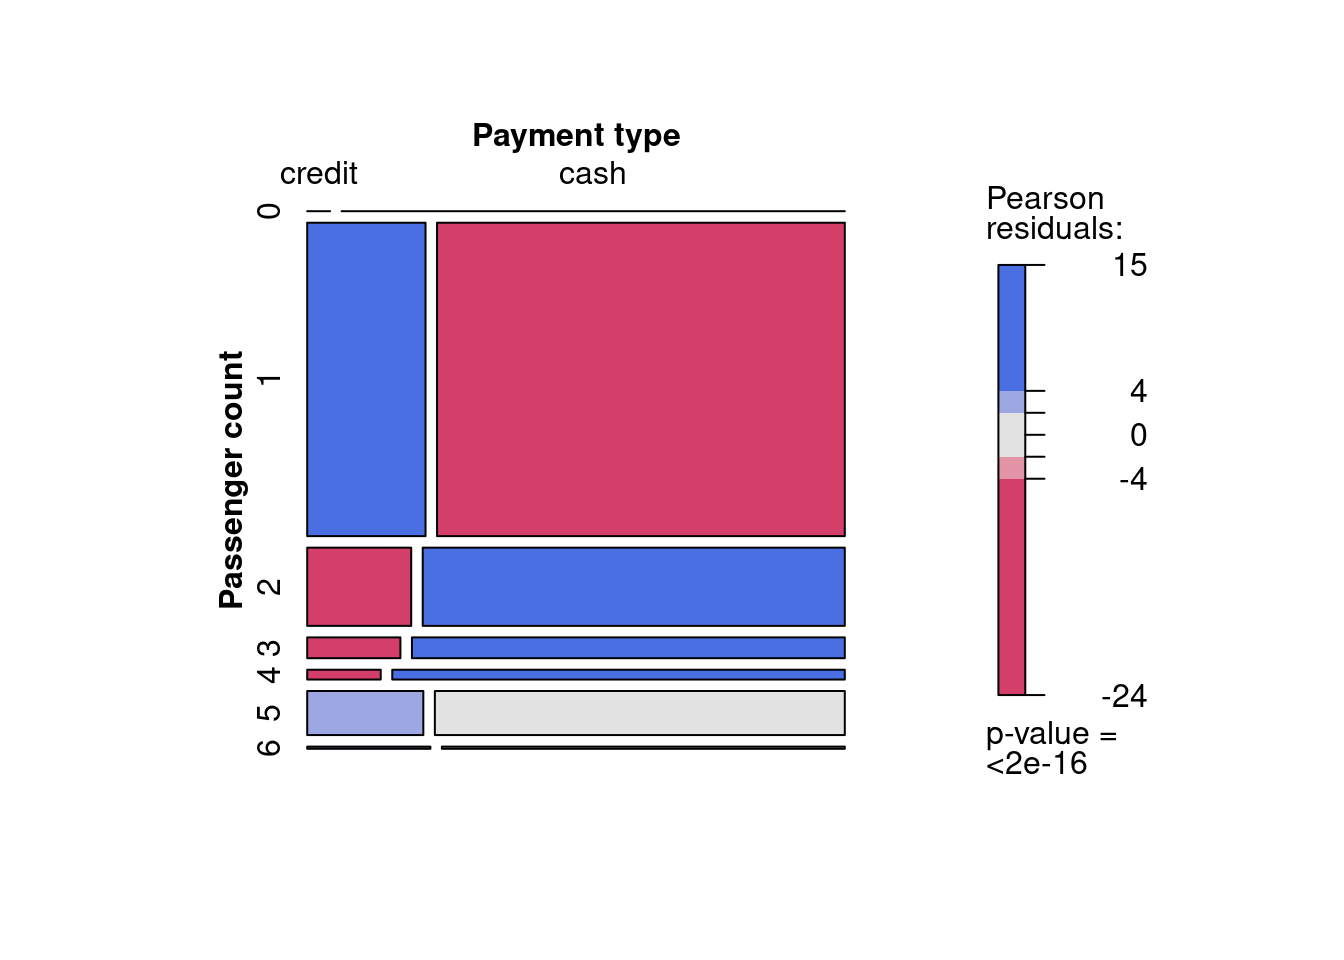
\includegraphics{bigdata_files/figure-latex/unnamed-chunk-95-1.pdf}

The plot suggests that trips involving more than one passenger tend to be paid rather by cash than by credit card.

\hypertarget{high-speed-in-memory-data-aggregation-with-data.table}{%
\subsection{\texorpdfstring{High-speed in-memory data aggregation with \texttt{data.table}}{High-speed in-memory data aggregation with data.table}}\label{high-speed-in-memory-data-aggregation-with-data.table}}

For large data sets that still fit into RAM, the \texttt{data.table}-package provides very fast and elegant functions to compute aggregate statistics.

\hypertarget{data-import-2}{%
\subsubsection{Data import}\label{data-import-2}}

We use the already familiar \texttt{fread()} to import the same first million observations from the January 2009 taxi trips records.

\begin{Shaded}
\begin{Highlighting}[]
\CommentTok{\# load packages}
\FunctionTok{library}\NormalTok{(data.table)}

\CommentTok{\# import data into RAM (needs around 200MB)}
\NormalTok{taxi }\OtherTok{\textless{}{-}} \FunctionTok{fread}\NormalTok{(}\StringTok{"data/tlc\_trips.csv"}\NormalTok{,}
              \AttributeTok{nrows =} \DecValTok{1000000}\NormalTok{)}
\end{Highlighting}
\end{Shaded}

\hypertarget{data-preparation}{%
\subsubsection{Data preparation}\label{data-preparation}}

We prepare/clean the data as in the \texttt{ff}-approach above.

\begin{Shaded}
\begin{Highlighting}[]
\CommentTok{\# first, we remove the empty vars V8 and V9}
\NormalTok{taxi}\SpecialCharTok{$}\NormalTok{V8 }\OtherTok{\textless{}{-}} \ConstantTok{NULL}
\NormalTok{taxi}\SpecialCharTok{$}\NormalTok{V9 }\OtherTok{\textless{}{-}} \ConstantTok{NULL}


\CommentTok{\# set covariate names according to the data dictionary}
\CommentTok{\# see https://www1.nyc.gov/assets/tlc/downloads/pdf/data\_dictionary\_trip\_records\_yellow.pdf}
\CommentTok{\# note instead of taxizonne ids, long/lat are provided}

\NormalTok{varnames }\OtherTok{\textless{}{-}} \FunctionTok{c}\NormalTok{(}\StringTok{"vendor\_id"}\NormalTok{,}
              \StringTok{"pickup\_time"}\NormalTok{,}
              \StringTok{"dropoff\_time"}\NormalTok{,}
              \StringTok{"passenger\_count"}\NormalTok{,}
              \StringTok{"trip\_distance"}\NormalTok{,}
              \StringTok{"start\_lat"}\NormalTok{,}
              \StringTok{"start\_long"}\NormalTok{,}
              \StringTok{"dest\_lat"}\NormalTok{,}
              \StringTok{"dest\_long"}\NormalTok{,}
              \StringTok{"payment\_type"}\NormalTok{,}
              \StringTok{"fare\_amount"}\NormalTok{,}
              \StringTok{"extra"}\NormalTok{,}
              \StringTok{"mta\_tax"}\NormalTok{,}
              \StringTok{"tip\_amount"}\NormalTok{,}
              \StringTok{"tolls\_amount"}\NormalTok{,}
              \StringTok{"total\_amount"}\NormalTok{)}
\FunctionTok{names}\NormalTok{(taxi) }\OtherTok{\textless{}{-}}\NormalTok{ varnames}

\CommentTok{\# clean the factor levels}
\NormalTok{taxi}\SpecialCharTok{$}\NormalTok{payment\_type }\OtherTok{\textless{}{-}} \FunctionTok{tolower}\NormalTok{(taxi}\SpecialCharTok{$}\NormalTok{payment\_type)}
\NormalTok{taxi}\SpecialCharTok{$}\NormalTok{payment\_type }\OtherTok{\textless{}{-}} \FunctionTok{factor}\NormalTok{(taxi}\SpecialCharTok{$}\NormalTok{payment\_type, }\AttributeTok{levels =} \FunctionTok{unique}\NormalTok{(taxi}\SpecialCharTok{$}\NormalTok{payment\_type))     }
\end{Highlighting}
\end{Shaded}

Note the simpler syntax of essentially doing the same thing, but all in-memory.

\hypertarget{data.table-syntax-for-split-apply-combine-operations}{%
\subsubsection{\texorpdfstring{\texttt{data.table}-syntax for `split-apply-combine' operations}{data.table-syntax for `split-apply-combine' operations}}\label{data.table-syntax-for-split-apply-combine-operations}}

With the \texttt{{[}{]}}-syntax we index/subset usual \texttt{data.frame} objects in R. When working with \texttt{data.table}s, much more can be done in the step of `sub-setting' the frame.\footnote{See \url{https://cran.r-project.org/web/packages/data.table/vignettes/datatable-intro.html} for a detailed introduction to the syntax.}

For example, we can directly compute on columns.

\begin{Shaded}
\begin{Highlighting}[]
\NormalTok{taxi[, }\FunctionTok{mean}\NormalTok{(tip\_amount}\SpecialCharTok{/}\NormalTok{total\_amount)]}
\end{Highlighting}
\end{Shaded}

\begin{verbatim}
## [1] 0.03452
\end{verbatim}

Moreover, in the same step, we can `split' the rows \emph{by} specific groups and apply the function to each subset.

\begin{Shaded}
\begin{Highlighting}[]
\NormalTok{taxi[, .(}\AttributeTok{percent\_tip =} \FunctionTok{mean}\NormalTok{((tip\_amount}\SpecialCharTok{/}\NormalTok{total\_amount)}\SpecialCharTok{*}\DecValTok{100}\NormalTok{)), by }\OtherTok{=}\NormalTok{ payment\_type]}
\end{Highlighting}
\end{Shaded}

\begin{verbatim}
##    payment_type percent_tip
## 1:         cash    0.005978
## 2:       credit   16.004173
## 3:    no charge    0.040433
## 4:      dispute    0.045660
\end{verbatim}

Similarly, we can use \texttt{data.table}'s \texttt{dcast()} for cross-tabulation-like operations.

\begin{Shaded}
\begin{Highlighting}[]
\FunctionTok{dcast}\NormalTok{(taxi[payment\_type }\SpecialCharTok{\%in\%} \FunctionTok{c}\NormalTok{(}\StringTok{"credit"}\NormalTok{, }\StringTok{"cash"}\NormalTok{)],}
\NormalTok{      passenger\_count}\SpecialCharTok{\textasciitilde{}}\NormalTok{payment\_type, }
      \AttributeTok{fun.aggregate =}\NormalTok{ length,}
      \AttributeTok{value.var =} \StringTok{"vendor\_id"}\NormalTok{)}
\end{Highlighting}
\end{Shaded}

\begin{verbatim}
##    passenger_count   cash credit
## 1:               0     44      2
## 2:               1 516828 149990
## 3:               2 133468  32891
## 4:               3  36439   7847
## 5:               4  17901   2909
## 6:               5  73027  20688
## 7:               6   3588   1097
\end{verbatim}

\hypertarget{data-storage-and-databases}{%
\chapter{Data Storage and Databases}\label{data-storage-and-databases}}

\hypertarget{big-data-storage}{%
\section{(Big) Data Storage}\label{big-data-storage}}

So far, we have primarily been concerned with situations in which a data set is too large to fit into RAM, making an analysis of these data either impossible or very slow (inefficient) when using standard tools. Thus, we have explored concepts and tools that help us use the available RAM (and virtual memory) most efficiently for data analysis tasks.

In this lecture, we are concerned with \((I)\) how we can store large data sets permanently on a mass storage device in an efficient way (here, efficient can be understood as `not taking up too much space') and \((II)\) how we can load (parts of) this data set in an efficient way (here, efficient\textasciitilde fast) for analysis.

We look at this problem in two situations:

\begin{itemize}
\tightlist
\item
  The data needs to be stored locally (e.g., on the hard disk of our laptop).
\item
  The data can be stored on a server `in the cloud'.
\end{itemize}

Various tools have been developed over the last few years to improve the efficiency of storing and accessing large amounts of data (see \citet{walkowiak_2016}, chapters 5 and 6 for an overview). Here, we focus on the basic concept of Relational Database Systems (RDBMS) and a well-known tool based on this concept, the Structured Query Language (SQL; more specifically, SQLite)

\hypertarget{rdbms-basics}{%
\section{RDBMS basics}\label{rdbms-basics}}

RDBMSs have two key features that tackle the two efficiency concerns mentioned above:

\begin{itemize}
\item
  The \emph{relational data model}: The overall data set is split by columns (covariates) into tables in order to reduce the storage of redundant variable-value repetitions. The resulting database tables are then linked via key-variables (unique identifiers). Thus (simply put), each type of entity on which observations exist resides in its own database table. Within this table, each observation has it's unique id. Keeping the data in such a structure is very efficient in terms of storage space used.
\item
  \emph{Indexing}: The key-columns of the database tables are indexed, meaning (in simple terms) ordered on disk. Indexing a table takes time but it has to be performed only once (unless the content of the table changes). The resulting index is then stored on disk as part of the database. These indices substantially reduce the number of disk accesses required to query/find specific observations. Thus, they make the loading of specific parts of the data for analysis much more efficient.
\end{itemize}

The loading/querying of data from an RDBMS typically involves the selection of specific observations (rows) and covariates (columns) from different tables. Due to the indexing, observations are selected efficiently, and the defined relations between tables (via keys) facilitate the joining of columns to a new table (the queried data).

\hypertarget{getting-started-with-rsqlite}{%
\section{Getting started with (R)SQLite}\label{getting-started-with-rsqlite}}

\href{https://sqlite.org/index.html}{SQLite} is a free full-featured SQL database engine and widely used across platforms and is typically pre-installed with Windows and OSX distributions. It is perfect to learn how to use RDBMSs/SQL. The R-package \texttt{RSQLite} embeds SQLite in R. That is, it provides functions that allow us to us SQLite directly from within R.

\hypertarget{first-steps-in-sqlite}{%
\subsection{First steps in SQLite}\label{first-steps-in-sqlite}}

In the terminal, we can directly call SQLite as a command-line tool (on most modern computers this is now \texttt{sqlite3}). In this short example, we set up our first SQLite database, using the command line. In the file structure of the course repository, we first switch to the data directory.

\begin{Shaded}
\begin{Highlighting}[]
\BuiltInTok{cd}\NormalTok{ materials/data }
\end{Highlighting}
\end{Shaded}

With one simple command, we both create a new SQLite database called \texttt{mydb.sqlite} and connect/run SQLite.

\begin{Shaded}
\begin{Highlighting}[]
\ExtensionTok{sqlite3}\NormalTok{ mydb.sqlite}
\end{Highlighting}
\end{Shaded}

This created a new file \texttt{mydb.sqlite} in our \texttt{data} directory. And we are now running \texttt{sqlite} in our terminal. But, the database is still empty. There are no tables in it. We can check the tables of a database with the following SQL command \texttt{.tables}.

\begin{Shaded}
\begin{Highlighting}[]
\NormalTok{.}\KeywordTok{tables}
\end{Highlighting}
\end{Shaded}

As expected, nothing is returned. Now, let's create our first table and import the \texttt{economics.csv} data set to it. In SQLite, it makes sense to first set up an empty table in which all column data types are defined before importing data from a CSV-file to it. If a CSV is directly imported to a new table (without type definitions), all columns will be set to \texttt{TEXT} by default.

\begin{Shaded}
\begin{Highlighting}[]
\CommentTok{{-}{-} Create the new table}
\KeywordTok{CREATE} \KeywordTok{TABLE}\NormalTok{ econ(}
\OtherTok{"date"} \DataTypeTok{DATE}\NormalTok{,}
\OtherTok{"pce"} \DataTypeTok{REAL}\NormalTok{,}
\OtherTok{"pop"} \DataTypeTok{INTEGER}\NormalTok{,}
\OtherTok{"psavert"} \DataTypeTok{REAL}\NormalTok{,}
\OtherTok{"uempmed"} \DataTypeTok{REAL}\NormalTok{,}
\OtherTok{"unemploy"} \DataTypeTok{INTEGER}
\NormalTok{);}

\CommentTok{{-}{-} prepare import}
\NormalTok{.}\KeywordTok{mode}\NormalTok{ csv}
\CommentTok{{-}{-} import data from csv}
\NormalTok{.import economics.csv econ}
\end{Highlighting}
\end{Shaded}

Now we can have a look at the new database table in SQLite. \texttt{.tables} shows that we now hove one table called \texttt{econ} in our database and \texttt{.schema} displays the structure of the new \texttt{econ} table.

\begin{verbatim}
.tables
\end{verbatim}

\begin{verbatim}
# econ
\end{verbatim}

\begin{verbatim}
.schema econ
\end{verbatim}

\begin{verbatim}
# CREATE TABLE econ(
# "date" DATE,
# "pce" REAL,
# "pop" INTEGER,
# "psavert" REAL,
# "uempmed" REAL,
# "unemploy" INTEGER
# );
\end{verbatim}

With this, we can actually start querying data with SQLite. In order to make the query results easier to read, we first set two options regarding how query results are displayed in the terminal. \texttt{.header\ on} enables the display of the column names in the returned query results. And \texttt{.mode\ columns} arranges the query results in columns.

\begin{Shaded}
\begin{Highlighting}[]
\NormalTok{.}\KeywordTok{header} \KeywordTok{on}
\end{Highlighting}
\end{Shaded}

\begin{Shaded}
\begin{Highlighting}[]
\NormalTok{.}\KeywordTok{mode} \KeywordTok{columns}
\end{Highlighting}
\end{Shaded}

In our first query, we select all (\texttt{*}) variable values of the observation of January 1968.

\begin{Shaded}
\begin{Highlighting}[]
\KeywordTok{select} \OperatorTok{*} \KeywordTok{from}\NormalTok{ econ }\KeywordTok{where} \DataTypeTok{date} \OperatorTok{=} \StringTok{\textquotesingle{}1968{-}01{-}01\textquotesingle{}}\NormalTok{;}
\end{Highlighting}
\end{Shaded}

\begin{table}

\caption{\label{tab:unnamed-chunk-109}1 records}
\centering
\begin{tabular}[t]{l|r|r|r|r|r}
\hline
date & pce & pop & psavert & uempmed & unemploy\\
\hline
1968-01-01 & 531.5 & 199808 & 11.7 & 5.1 & 2878\\
\hline
\end{tabular}
\end{table}

Now let's select all year/months in which there were more than 15 million unemployed, ordered by date.

\begin{Shaded}
\begin{Highlighting}[]
\KeywordTok{select} \DataTypeTok{date} \KeywordTok{from}\NormalTok{ econ }
\KeywordTok{where}\NormalTok{ unemploy }\OperatorTok{\textgreater{}} \DecValTok{15000}
\KeywordTok{order} \KeywordTok{by} \DataTypeTok{date}\NormalTok{;}
\end{Highlighting}
\end{Shaded}

\begin{table}

\caption{\label{tab:unnamed-chunk-110}Displaying records 1 - 10}
\centering
\begin{tabular}[t]{l}
\hline
date\\
\hline
2009-09-01\\
\hline
2009-10-01\\
\hline
2009-11-01\\
\hline
2009-12-01\\
\hline
2010-01-01\\
\hline
2010-02-01\\
\hline
2010-03-01\\
\hline
2010-04-01\\
\hline
2010-11-01\\
\hline
date\\
\hline
\end{tabular}
\end{table}

When done working with the database, we can exit SQLite with the \texttt{.quit} command.

\hypertarget{indices-and-joins}{%
\subsection{Indices and joins}\label{indices-and-joins}}

So far we have only had a look at the basic functionality of SQLite. But we have not really looked at the key features of an RDBMS (indexing and relations between tables).

We set up a new database called \texttt{air.sqlite} and import the csv-file \texttt{flights.csv} (used in previous lectures) as a first table.

\begin{Shaded}
\begin{Highlighting}[]
\CommentTok{\# create database and run sqlite}
\ExtensionTok{sqlite3}\NormalTok{ air.sqlite}
\end{Highlighting}
\end{Shaded}

\begin{Shaded}
\begin{Highlighting}[]
\CommentTok{{-}{-} import csvs}
\NormalTok{.}\KeywordTok{mode}\NormalTok{ csv}
\NormalTok{.import flights.csv flights}
\end{Highlighting}
\end{Shaded}

Again, we can check if everything worked out well with \texttt{.tables} and \texttt{.schema}.

\begin{Shaded}
\begin{Highlighting}[]
\NormalTok{.}\KeywordTok{tables}
\NormalTok{.}\KeywordTok{schema}\NormalTok{ flights}
\end{Highlighting}
\end{Shaded}

In \texttt{flights}, each row describes a flight (the day it took place, its origin, its destination etc.). It contains a covariate \texttt{carrier} containing the unique ID of the respective airline/carrier carrying out the flight as well as the covariates \texttt{origin} and \texttt{dest}. The latter two variables contain the unique IATA-codes of the airports from which the flights departed and where they arrived, respectively. In \texttt{flights} we thus have observations at the level of individual flights.

Now we extend our database in a meaningful way, following the relational data model idea. From the {[}ASA's website{]}, we download two additional csv files containing data that relate to the flights table:

\begin{itemize}
\tightlist
\item
  \href{http://stat-computing.org/dataexpo/2009/airports.csv}{\texttt{airports.csv}}: Describes the locations of US Airports (relates to \texttt{origin} and \texttt{dest}).
\item
  \href{http://stat-computing.org/dataexpo/2009/carriers.csv}{\texttt{carriers.csv}}: A listing of carrier codes with full names (relates to the \texttt{carrier}-column in \texttt{flights}.
\end{itemize}

In this code example, the two csvs have already been downloaded to the \texttt{materials/data}-folder.

\begin{Shaded}
\begin{Highlighting}[]
\CommentTok{{-}{-} import airport data}
\NormalTok{.}\KeywordTok{mode}\NormalTok{ csv}
\NormalTok{.import airports.csv airports}
\NormalTok{.import carriers.csv carriers}

\CommentTok{{-}{-} inspect the result}
\NormalTok{.}\KeywordTok{tables}
\NormalTok{.}\KeywordTok{schema}\NormalTok{ airports}
\NormalTok{.}\KeywordTok{schema}\NormalTok{ carriers}
\end{Highlighting}
\end{Shaded}

Now we can run our first query involving the relation between tables. The aim of the exercise is to query flights data (information on departure delays per flight number and date; from the \texttt{flights}-table) for all \texttt{United\ Air\ Lines\ Inc.}-flights (information from the \texttt{carriers} table ) departing from \texttt{Newark\ Intl} airport (information from the \texttt{airports}-table). In addition, we want the resulting table ordered by flight number. For the sake of the exercise, we only show the first 10 results of this query (\texttt{LIMIT\ 10}).

\begin{Shaded}
\begin{Highlighting}[]
\KeywordTok{SELECT} 
\DataTypeTok{year}\NormalTok{,}
\DataTypeTok{month}\NormalTok{, }
\DataTypeTok{day}\NormalTok{,}
\NormalTok{dep\_delay,}
\NormalTok{flight}
\KeywordTok{FROM}\NormalTok{ (flights }\KeywordTok{INNER} \KeywordTok{JOIN}\NormalTok{ airports }\KeywordTok{ON}\NormalTok{ flights.origin}\OperatorTok{=}\NormalTok{airports.iata) }
\KeywordTok{INNER} \KeywordTok{JOIN}\NormalTok{ carriers }\KeywordTok{ON}\NormalTok{ flights.carrier }\OperatorTok{=}\NormalTok{ carriers.Code}
\KeywordTok{WHERE}\NormalTok{ carriers.Description }\OperatorTok{=} \StringTok{\textquotesingle{}United Air Lines Inc.\textquotesingle{}}
\KeywordTok{AND}\NormalTok{ airports.airport }\OperatorTok{=} \StringTok{\textquotesingle{}Newark Intl\textquotesingle{}}
\KeywordTok{ORDER} \KeywordTok{BY}\NormalTok{ flight}
\KeywordTok{LIMIT} \DecValTok{10}\NormalTok{;}
\end{Highlighting}
\end{Shaded}

\begin{table}

\caption{\label{tab:unnamed-chunk-117}Displaying records 1 - 10}
\centering
\begin{tabular}[t]{r|r|r|r|r}
\hline
year & month & day & dep\_delay & flight\\
\hline
2013 & 1 & 4 & 0 & 1\\
\hline
2013 & 1 & 5 & -2 & 1\\
\hline
2013 & 3 & 6 & 1 & 1\\
\hline
2013 & 2 & 13 & -2 & 3\\
\hline
2013 & 2 & 16 & -9 & 3\\
\hline
2013 & 2 & 20 & 3 & 3\\
\hline
2013 & 2 & 23 & -5 & 3\\
\hline
2013 & 2 & 26 & 24 & 3\\
\hline
2013 & 2 & 27 & 10 & 3\\
\hline
2013 & 1 & 5 & 3 & 10\\
\hline
\end{tabular}
\end{table}

Note that this query has been executed without indexing any of the tables first. Thus SQLite could not take any `shortcuts' when matching the ID columns in order to join the tables for the query output. That is, SQLite had to scan the entire columns to find the matches. Now we index the respective id columns and re-run the query

\begin{Shaded}
\begin{Highlighting}[]
\KeywordTok{CREATE} \KeywordTok{INDEX}\NormalTok{ iata\_airports }\KeywordTok{ON}\NormalTok{ airports (iata);}
\KeywordTok{CREATE} \KeywordTok{INDEX}\NormalTok{ origin\_flights }\KeywordTok{ON}\NormalTok{ flights (origin);}
\KeywordTok{CREATE} \KeywordTok{INDEX}\NormalTok{ carrier\_flights }\KeywordTok{ON}\NormalTok{ flights (carrier);}
\KeywordTok{CREATE} \KeywordTok{INDEX}\NormalTok{ code\_carriers }\KeywordTok{ON}\NormalTok{ carriers (code);}
\end{Highlighting}
\end{Shaded}

Now we can re-run the query from above. Note that SQLite optimizes the efficiency of the query without our explicit instructions. If there are indices it can use to speed up the query, it will do so.

\begin{Shaded}
\begin{Highlighting}[]
\KeywordTok{SELECT} 
\DataTypeTok{year}\NormalTok{,}
\DataTypeTok{month}\NormalTok{, }
\DataTypeTok{day}\NormalTok{,}
\NormalTok{dep\_delay,}
\NormalTok{flight}
\KeywordTok{FROM}\NormalTok{ (flights }\KeywordTok{INNER} \KeywordTok{JOIN}\NormalTok{ airports }\KeywordTok{ON}\NormalTok{ flights.origin}\OperatorTok{=}\NormalTok{airports.iata) }
\KeywordTok{INNER} \KeywordTok{JOIN}\NormalTok{ carriers }\KeywordTok{ON}\NormalTok{ flights.carrier }\OperatorTok{=}\NormalTok{ carriers.Code}
\KeywordTok{WHERE}\NormalTok{ carriers.Description }\OperatorTok{=} \StringTok{\textquotesingle{}United Air Lines Inc.\textquotesingle{}}
\KeywordTok{AND}\NormalTok{ airports.airport }\OperatorTok{=} \StringTok{\textquotesingle{}Newark Intl\textquotesingle{}}
\KeywordTok{ORDER} \KeywordTok{BY}\NormalTok{ flight}
\KeywordTok{LIMIT} \DecValTok{10}\NormalTok{;}
\end{Highlighting}
\end{Shaded}

\begin{table}

\caption{\label{tab:unnamed-chunk-119}Displaying records 1 - 10}
\centering
\begin{tabular}[t]{r|r|r|r|r}
\hline
year & month & day & dep\_delay & flight\\
\hline
2013 & 1 & 4 & 0 & 1\\
\hline
2013 & 1 & 5 & -2 & 1\\
\hline
2013 & 3 & 6 & 1 & 1\\
\hline
2013 & 2 & 13 & -2 & 3\\
\hline
2013 & 2 & 16 & -9 & 3\\
\hline
2013 & 2 & 20 & 3 & 3\\
\hline
2013 & 2 & 23 & -5 & 3\\
\hline
2013 & 2 & 26 & 24 & 3\\
\hline
2013 & 2 & 27 & 10 & 3\\
\hline
2013 & 1 & 5 & 3 & 10\\
\hline
\end{tabular}
\end{table}

You find the final \texttt{air.sqlite}, including all the indices and tables as \texttt{materials/data/air\_final.sqlite} in the course's code repository.

\hypertarget{sqlite-from-within-r}{%
\section{SQLite from within R}\label{sqlite-from-within-r}}

The \texttt{RSQLite}-package provides various R functions to control basically all of SQLite's functionalities from within R. In the following example, we explore how \texttt{RSQLite} can be used to set up and query the \texttt{air.sqlite} shown in the example above.

\hypertarget{creating-a-new-database-with-rsqlite}{%
\subsection{\texorpdfstring{Creating a new database with \texttt{RSQLite}}{Creating a new database with RSQLite}}\label{creating-a-new-database-with-rsqlite}}

Similarly to the raw SQLite-syntax, connecting to a database that does not exist yet, actually creates this (empty database). Note that for all interactions with the database from within R, we need to refer to the connection (here: \texttt{con\_air}).

\begin{Shaded}
\begin{Highlighting}[]
\CommentTok{\# load packages}
\FunctionTok{library}\NormalTok{(RSQLite)}

\CommentTok{\# initiate the database}
\NormalTok{con\_air }\OtherTok{\textless{}{-}} \FunctionTok{dbConnect}\NormalTok{(}\FunctionTok{SQLite}\NormalTok{(), }\StringTok{"data/air.sqlite"}\NormalTok{)}
\end{Highlighting}
\end{Shaded}

\hypertarget{importing-data}{%
\subsection{Importing data}\label{importing-data}}

With \texttt{RSQLite} we can easily add \texttt{data.frame}s as SQLite tables to the database.

\begin{Shaded}
\begin{Highlighting}[]
\CommentTok{\# import data into current R sesssion}
\NormalTok{flights }\OtherTok{\textless{}{-}} \FunctionTok{fread}\NormalTok{(}\StringTok{"data/flights.csv"}\NormalTok{)}
\NormalTok{airports }\OtherTok{\textless{}{-}} \FunctionTok{fread}\NormalTok{(}\StringTok{"data/airports.csv"}\NormalTok{)}
\NormalTok{carriers }\OtherTok{\textless{}{-}} \FunctionTok{fread}\NormalTok{(}\StringTok{"data/carriers.csv"}\NormalTok{)}

\CommentTok{\# add tables to database}
\FunctionTok{dbWriteTable}\NormalTok{(con\_air, }\StringTok{"flights"}\NormalTok{, flights)}
\FunctionTok{dbWriteTable}\NormalTok{(con\_air, }\StringTok{"airports"}\NormalTok{, airports)}
\FunctionTok{dbWriteTable}\NormalTok{(con\_air, }\StringTok{"carriers"}\NormalTok{, carriers)}
\end{Highlighting}
\end{Shaded}

\hypertarget{issue-queries}{%
\subsection{Issue queries}\label{issue-queries}}

Now we can query the database from within R. By default, \texttt{RSQLite} returns the query results as \texttt{data.frame}s. Queries are simply character strings written in SQLite.

\begin{Shaded}
\begin{Highlighting}[]
\CommentTok{\# define query}
\NormalTok{delay\_query }\OtherTok{\textless{}{-}}
\StringTok{"SELECT }
\StringTok{year,}
\StringTok{month, }
\StringTok{day,}
\StringTok{dep\_delay,}
\StringTok{flight}
\StringTok{FROM (flights INNER JOIN airports ON flights.origin=airports.iata) }
\StringTok{INNER JOIN carriers ON flights.carrier = carriers.Code}
\StringTok{WHERE carriers.Description = \textquotesingle{}United Air Lines Inc.\textquotesingle{}}
\StringTok{AND airports.airport = \textquotesingle{}Newark Intl\textquotesingle{}}
\StringTok{ORDER BY flight}
\StringTok{LIMIT 10;}
\StringTok{"}

\CommentTok{\# issue query}
\NormalTok{delays\_df }\OtherTok{\textless{}{-}} \FunctionTok{dbGetQuery}\NormalTok{(con\_air, delay\_query)}
\NormalTok{delays\_df}
\end{Highlighting}
\end{Shaded}

\begin{verbatim}
##    year month day dep_delay flight
## 1  2013     1   4         0      1
## 2  2013     1   5        -2      1
## 3  2013     3   6         1      1
## 4  2013     2  13        -2      3
## 5  2013     2  16        -9      3
## 6  2013     2  20         3      3
## 7  2013     2  23        -5      3
## 8  2013     2  26        24      3
## 9  2013     2  27        10      3
## 10 2013     1   5         3     10
\end{verbatim}

\hypertarget{big-data-visualization}{%
\chapter{(Big) Data Visualization}\label{big-data-visualization}}

\hypertarget{data-set}{%
\section{Data Set}\label{data-set}}

In this tutorial we will work with the TLC data used in the data aggregation session. The raw data consists of several monthly CSV-files and can be downloaded via the \href{https://www1.nyc.gov/site/tlc/about/tlc-trip-record-data.page}{TLC's website}. Again, we work only with the first million observations.

In order to better understand the large data set at hand (particularly regarding the determinants of tips paid) we use \texttt{ggplot2} to visualize some key aspects of the data.

First, let's look at the raw relationship between fare paid and the tip paid. We set up the canvas with \texttt{ggplot}.

\begin{Shaded}
\begin{Highlighting}[]
\CommentTok{\# load packages}
\FunctionTok{library}\NormalTok{(ggplot2)}

\CommentTok{\# set up the canvas}
\NormalTok{taxiplot }\OtherTok{\textless{}{-}} \FunctionTok{ggplot}\NormalTok{(taxi, }\FunctionTok{aes}\NormalTok{(}\AttributeTok{y=}\NormalTok{tip\_amount, }\AttributeTok{x=}\NormalTok{ fare\_amount)) }
\NormalTok{taxiplot}
\end{Highlighting}
\end{Shaded}

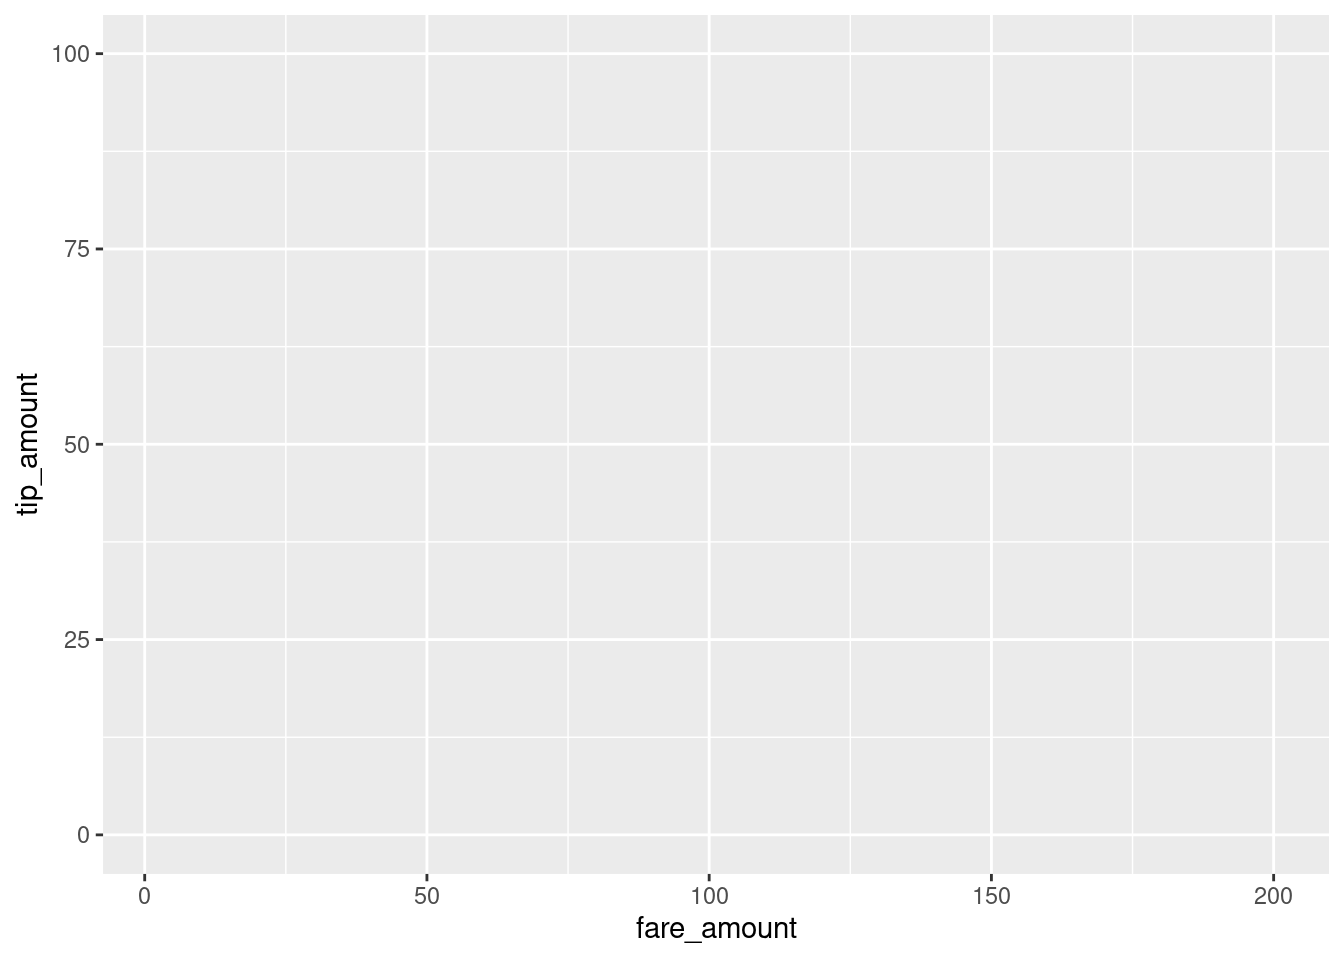
\includegraphics{bigdata_files/figure-latex/unnamed-chunk-125-1.pdf}

Now we visualize the co-distribution of the two variables with a simple scatter-plot.

\begin{Shaded}
\begin{Highlighting}[]
\CommentTok{\# simple x/y plot}
\NormalTok{taxiplot }\SpecialCharTok{+}
     \FunctionTok{geom\_point}\NormalTok{()}
\end{Highlighting}
\end{Shaded}

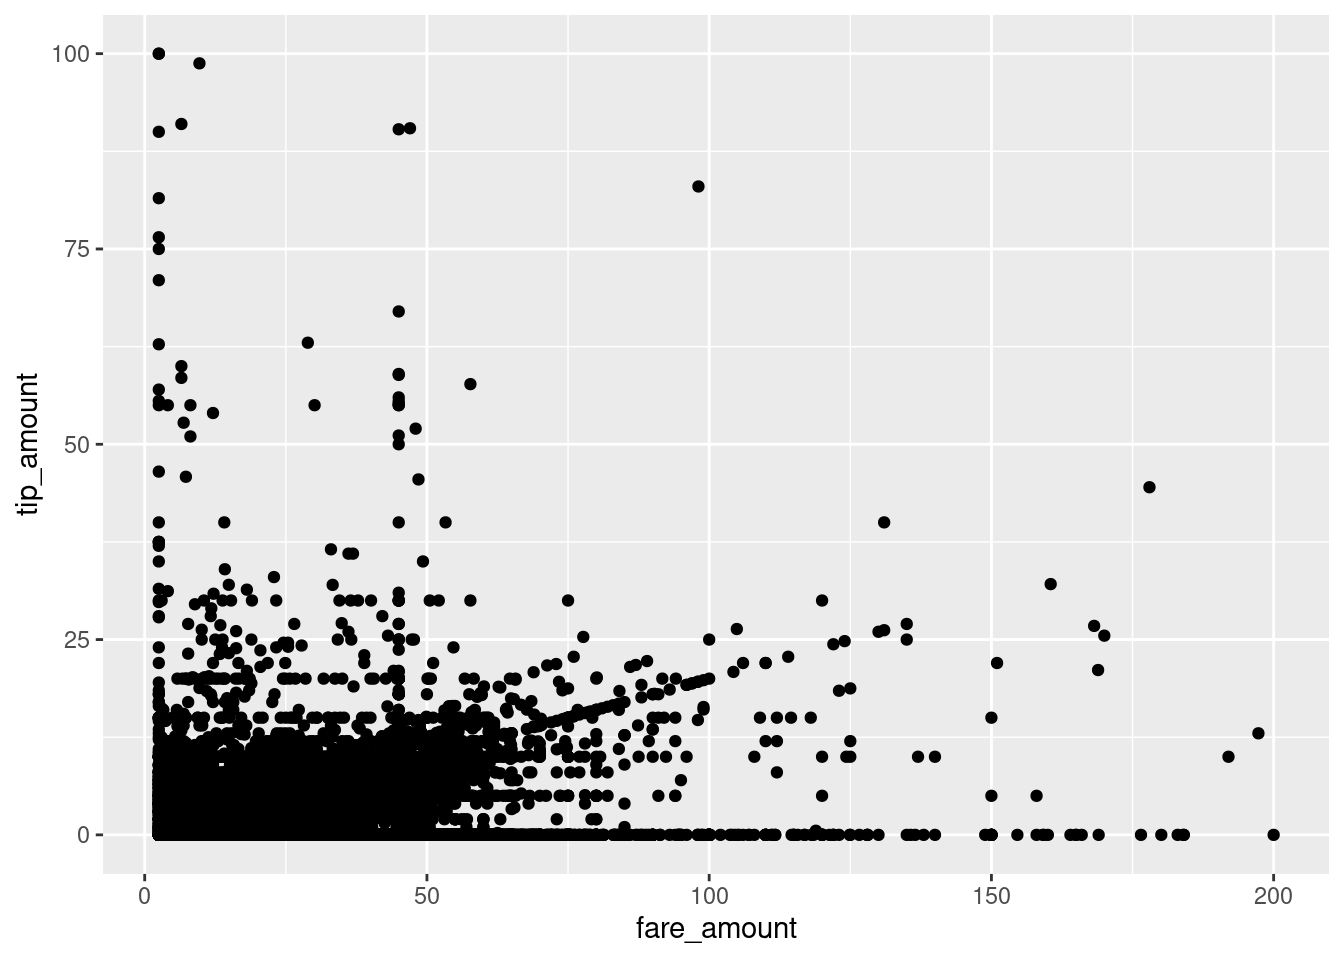
\includegraphics{bigdata_files/figure-latex/unnamed-chunk-126-1.pdf}

Note that this took quite a while, as R had to literally plot one million dots on the canvas. Moreover many dots fall within the same area, making it impossible to recognize how much mass there actually is. This is typical for visualization exercises with large data sets. One way to improve this, is by making the dots more transparent by setting the \texttt{alpha} parameter.

\begin{Shaded}
\begin{Highlighting}[]
\CommentTok{\# simple x/y plot}
\NormalTok{taxiplot }\SpecialCharTok{+}
     \FunctionTok{geom\_point}\NormalTok{(}\AttributeTok{alpha=}\FloatTok{0.2}\NormalTok{)}
\end{Highlighting}
\end{Shaded}

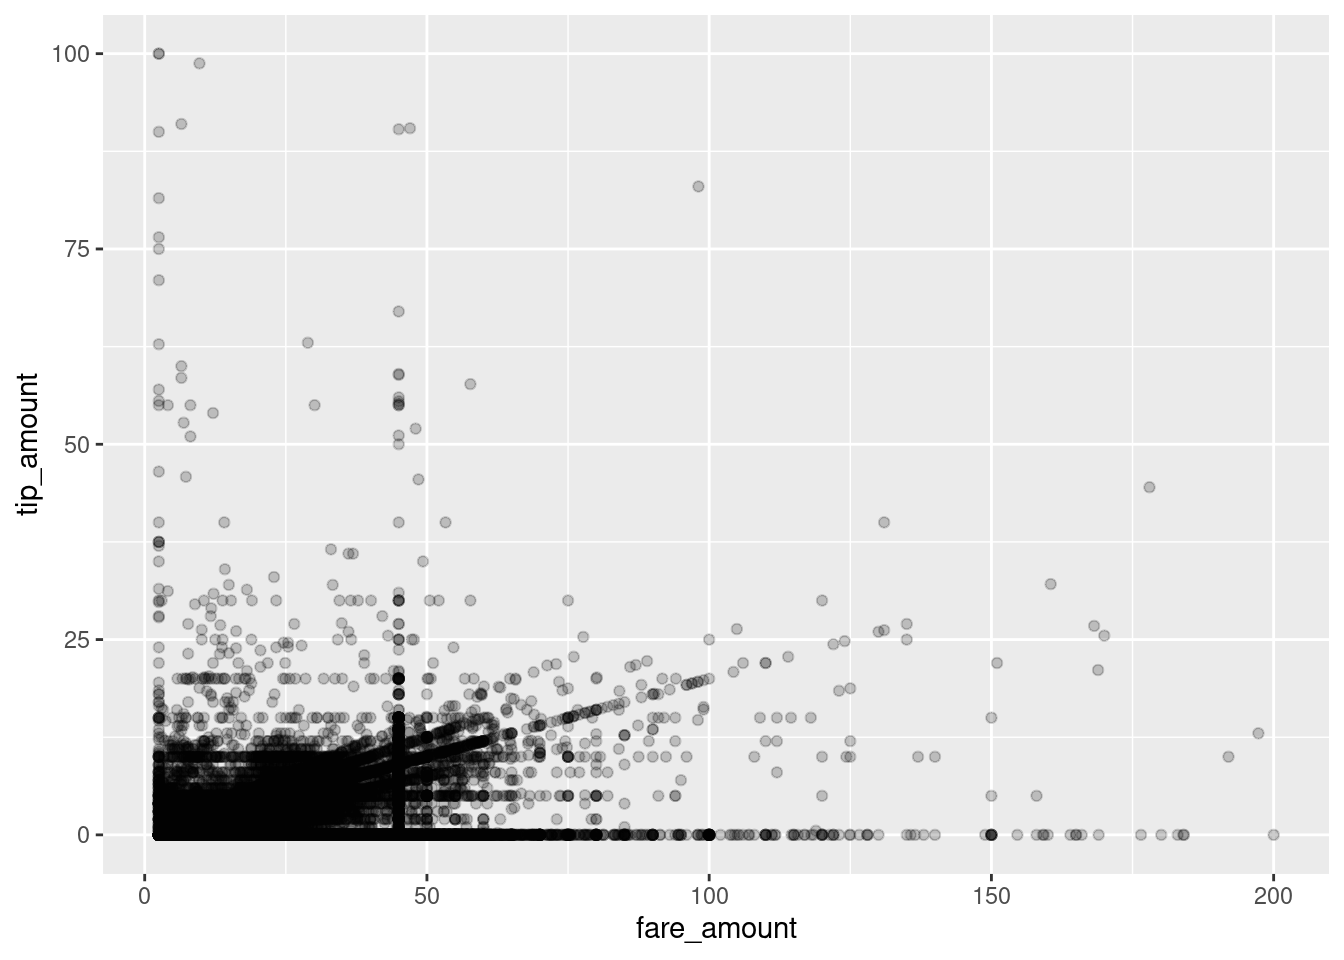
\includegraphics{bigdata_files/figure-latex/unnamed-chunk-127-1.pdf}

Alternatively, we can compute two-dimensional bins. Thereby, the canvas is split into rectangles and the number of observations falling into each respective rectangle is computed. The visualization is based on plotting the rectangles with counts greater than 0 and the shading of the rectangles indicates the count values.

\begin{Shaded}
\begin{Highlighting}[]
\CommentTok{\# 2{-}dimensional bins}
\NormalTok{taxiplot }\SpecialCharTok{+}
     \FunctionTok{geom\_bin2d}\NormalTok{()}
\end{Highlighting}
\end{Shaded}

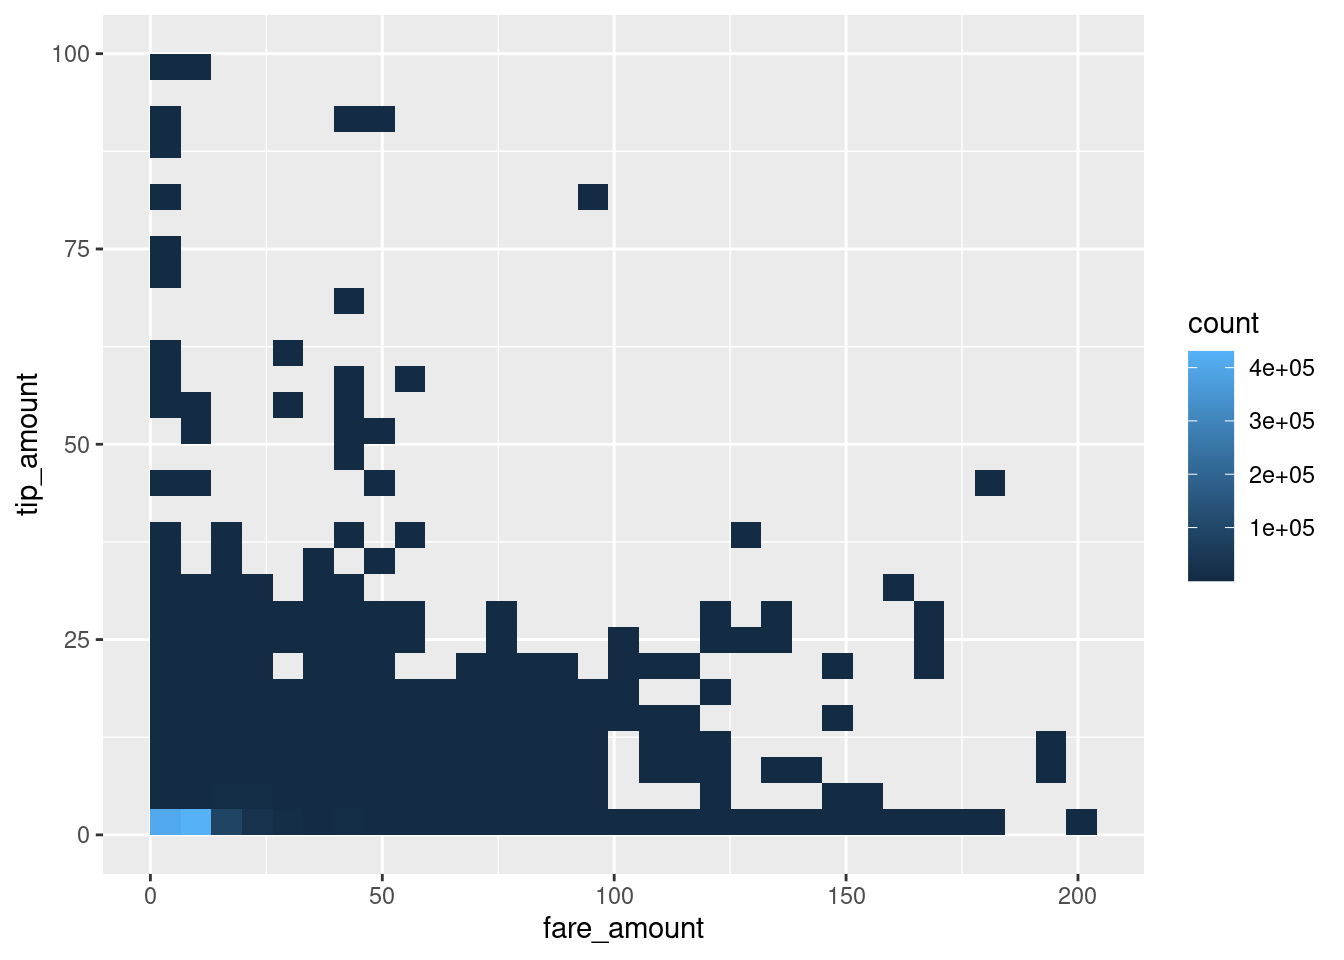
\includegraphics{bigdata_files/figure-latex/unnamed-chunk-128-1.pdf}

A large part of the tip/fare observations seem to be in the very lower-left corner of the pane, while most other trips seem to be evenly distributed. However, we fail to see slighter differences in this visualization. In order to reduce the dominance of the 2d-bins with very high counts, we display the natural logarithm of counts and display the bins as points.

\begin{Shaded}
\begin{Highlighting}[]
\CommentTok{\# 2{-}dimensional bins}
\NormalTok{taxiplot }\SpecialCharTok{+}
     \FunctionTok{stat\_bin\_2d}\NormalTok{(}\AttributeTok{geom=}\StringTok{"point"}\NormalTok{,}
                 \AttributeTok{mapping=} \FunctionTok{aes}\NormalTok{(}\AttributeTok{size =} \FunctionTok{log}\NormalTok{(..count..))) }\SpecialCharTok{+}
     \FunctionTok{guides}\NormalTok{(}\AttributeTok{fill =} \ConstantTok{FALSE}\NormalTok{)}
\end{Highlighting}
\end{Shaded}

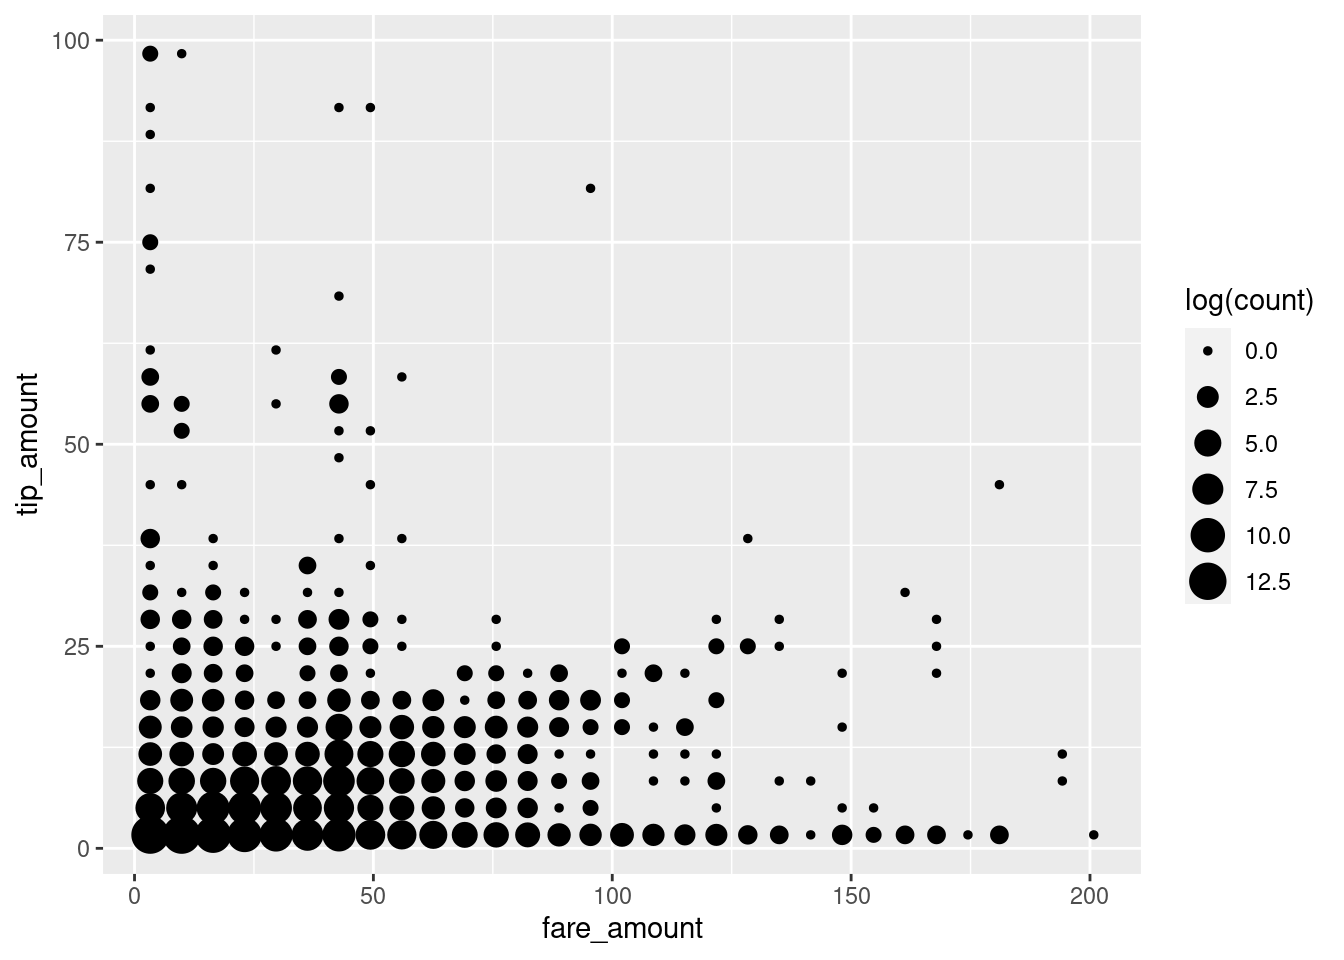
\includegraphics{bigdata_files/figure-latex/unnamed-chunk-129-1.pdf}

We note that there are many cases with very low fare amounts, many cases with no or hardly any tip, and quite a lot of cases with very high tip amounts (in relation to the rather low fare amount). In the following, we dissect this picture by having a closer look at `typical' tip amounts and whether they differ by type of payment.

\begin{Shaded}
\begin{Highlighting}[]
\CommentTok{\# compute frequency of per tip amount and payment method}
\NormalTok{taxi[, n\_same\_tip}\SpecialCharTok{:}\ErrorTok{=}\NormalTok{ .N, by}\OtherTok{=} \FunctionTok{c}\NormalTok{(}\StringTok{"tip\_amount"}\NormalTok{, }\StringTok{"payment\_type"}\NormalTok{)]}
\NormalTok{frequencies }\OtherTok{\textless{}{-}} \FunctionTok{unique}\NormalTok{(taxi[payment\_type }\SpecialCharTok{\%in\%} \FunctionTok{c}\NormalTok{(}\StringTok{"credit"}\NormalTok{, }\StringTok{"cash"}\NormalTok{),}
                           \FunctionTok{c}\NormalTok{(}\StringTok{"n\_same\_tip"}\NormalTok{, }\StringTok{"tip\_amount"}\NormalTok{, }\StringTok{"payment\_type"}\NormalTok{)][}\FunctionTok{order}\NormalTok{(n\_same\_tip, }\AttributeTok{decreasing =} \ConstantTok{TRUE}\NormalTok{)])}


\CommentTok{\# plot top 20 frequent tip amounts}
\NormalTok{fare }\OtherTok{\textless{}{-}} \FunctionTok{ggplot}\NormalTok{(}\AttributeTok{data =}\NormalTok{ frequencies[}\DecValTok{1}\SpecialCharTok{:}\DecValTok{20}\NormalTok{], }\FunctionTok{aes}\NormalTok{(}\AttributeTok{x =} \FunctionTok{factor}\NormalTok{(tip\_amount), }\AttributeTok{y =}\NormalTok{ n\_same\_tip)) }
\NormalTok{fare }\SpecialCharTok{+} \FunctionTok{geom\_bar}\NormalTok{(}\AttributeTok{stat =} \StringTok{"identity"}\NormalTok{) }
\end{Highlighting}
\end{Shaded}

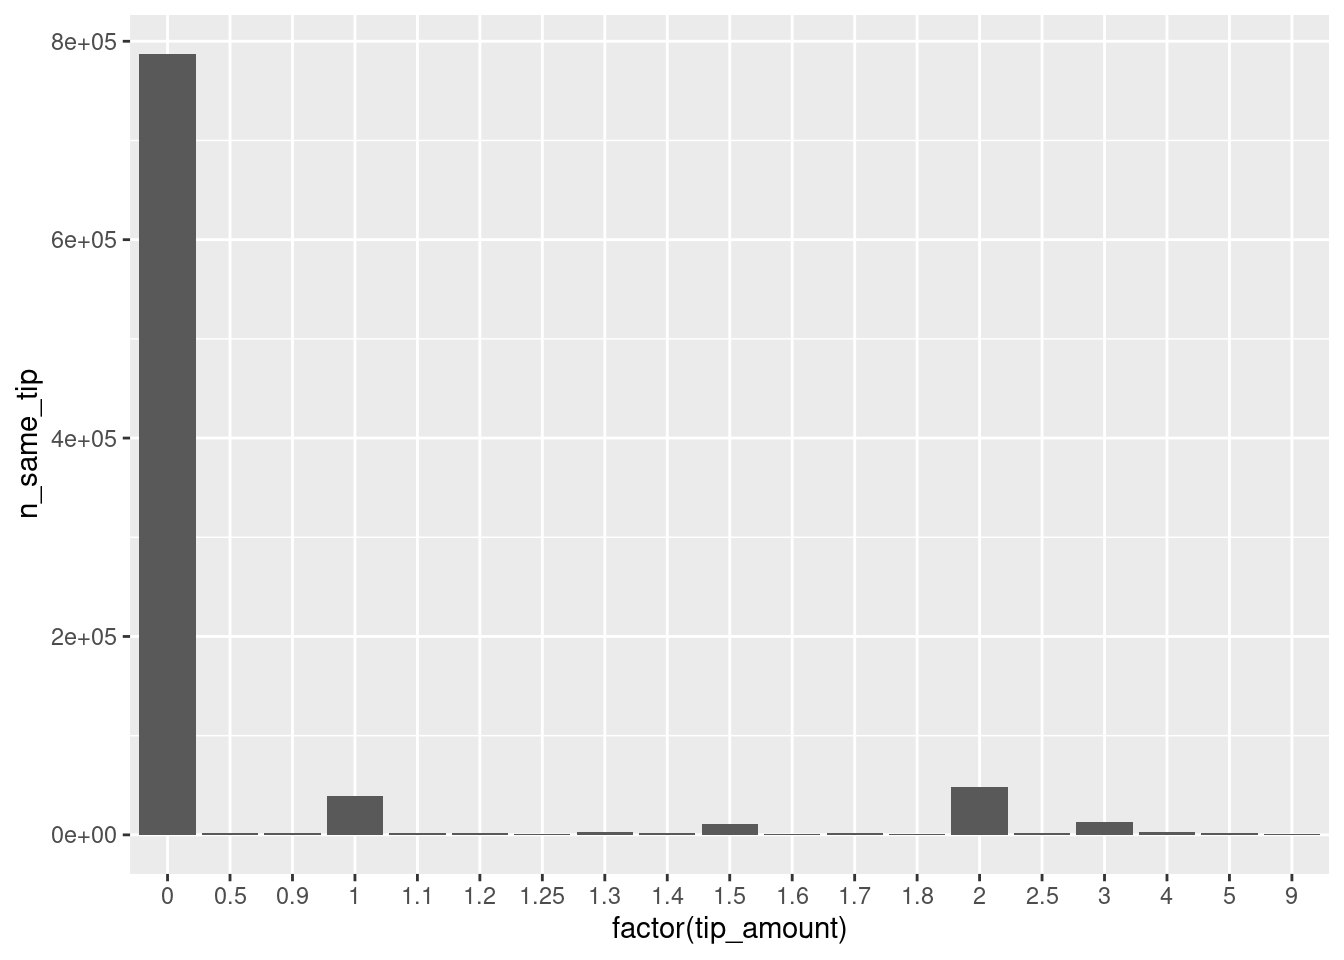
\includegraphics{bigdata_files/figure-latex/unnamed-chunk-130-1.pdf}

Indeed, paying no tip at all is quite frequent, overall.\footnote{Or, could there be another explanation for this pattern in the data?} The bar plot also indicates that there seem to be some `focal points' in the amount of tips paid. Clearly, paying one USD or two USD is more common than paying fractions. However, fractions of dollars might be more likely if tips are paid in cash and customers simply add some loose change to the fare amount paid.

\begin{Shaded}
\begin{Highlighting}[]
\NormalTok{fare }\SpecialCharTok{+} \FunctionTok{geom\_bar}\NormalTok{(}\AttributeTok{stat =} \StringTok{"identity"}\NormalTok{) }\SpecialCharTok{+} 
     \FunctionTok{facet\_wrap}\NormalTok{(}\StringTok{"payment\_type"}\NormalTok{) }
\end{Highlighting}
\end{Shaded}

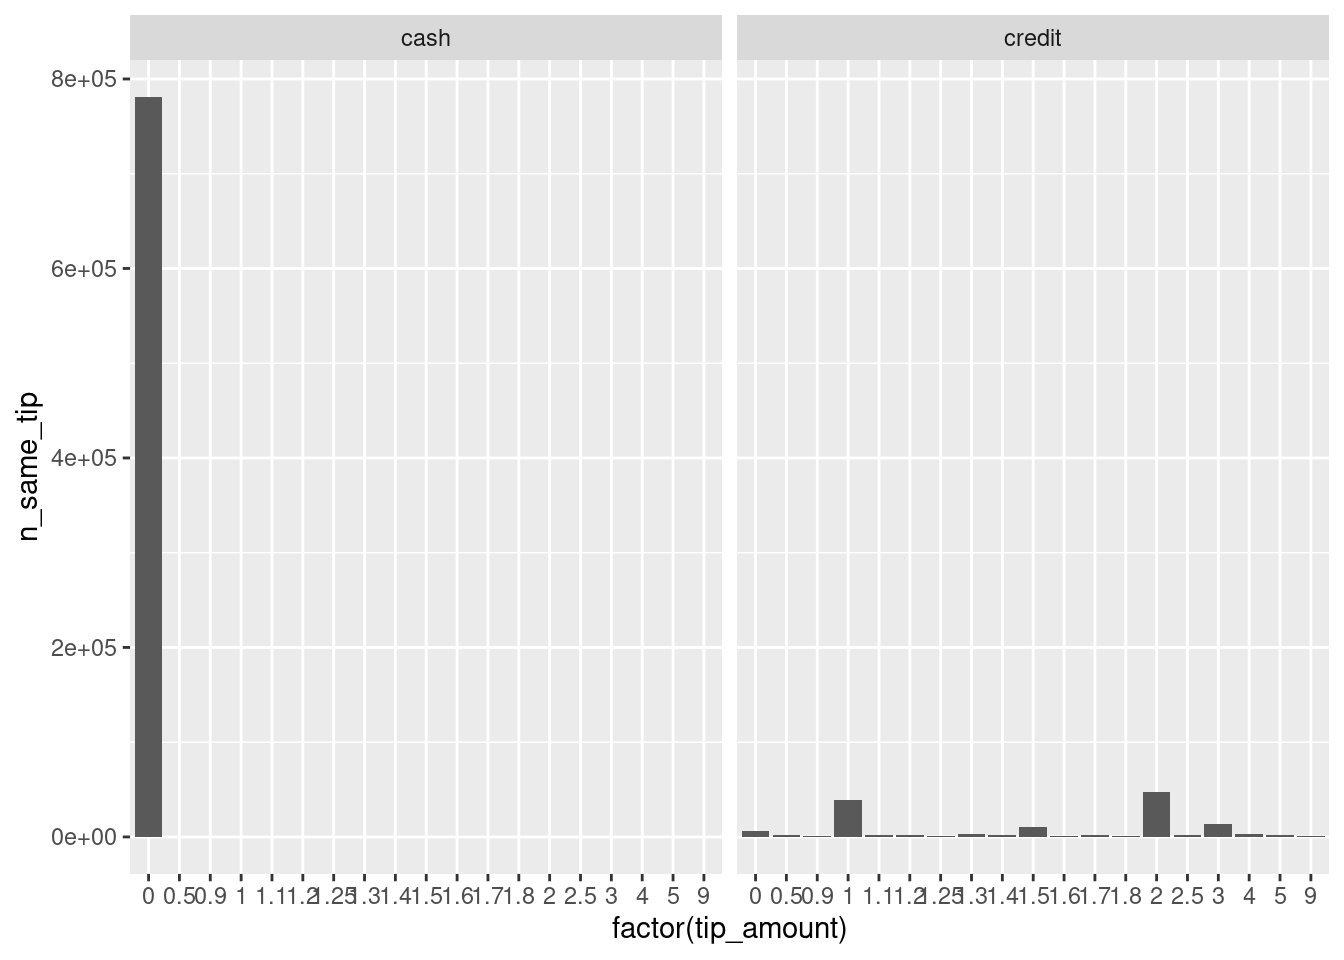
\includegraphics{bigdata_files/figure-latex/unnamed-chunk-131-1.pdf}

Clearly, it looks like trips paid in cash tend not to be tipped (at least in this subsample).

Let's try to tease this information out of the initial points plot. Trips paid in cash are often not tipped, we thus should indicate the payment method. Moreover, tips paid in full dollar amounts might indicate a habit.

\begin{Shaded}
\begin{Highlighting}[]
\CommentTok{\# indicate natural numbers}
\NormalTok{taxi[, dollar\_paid }\SpecialCharTok{:}\ErrorTok{=} \FunctionTok{ifelse}\NormalTok{(tip\_amount }\SpecialCharTok{==} \FunctionTok{round}\NormalTok{(tip\_amount,}\DecValTok{0}\NormalTok{), }\StringTok{"Full"}\NormalTok{, }\StringTok{"Fraction"}\NormalTok{),]}


\CommentTok{\# extended x/y plot}
\NormalTok{taxiplot }\SpecialCharTok{+}
     \FunctionTok{geom\_point}\NormalTok{(}\AttributeTok{alpha=}\FloatTok{0.2}\NormalTok{, }\FunctionTok{aes}\NormalTok{(}\AttributeTok{color=}\NormalTok{payment\_type)) }\SpecialCharTok{+}
     \FunctionTok{facet\_wrap}\NormalTok{(}\StringTok{"dollar\_paid"}\NormalTok{)}
\end{Highlighting}
\end{Shaded}

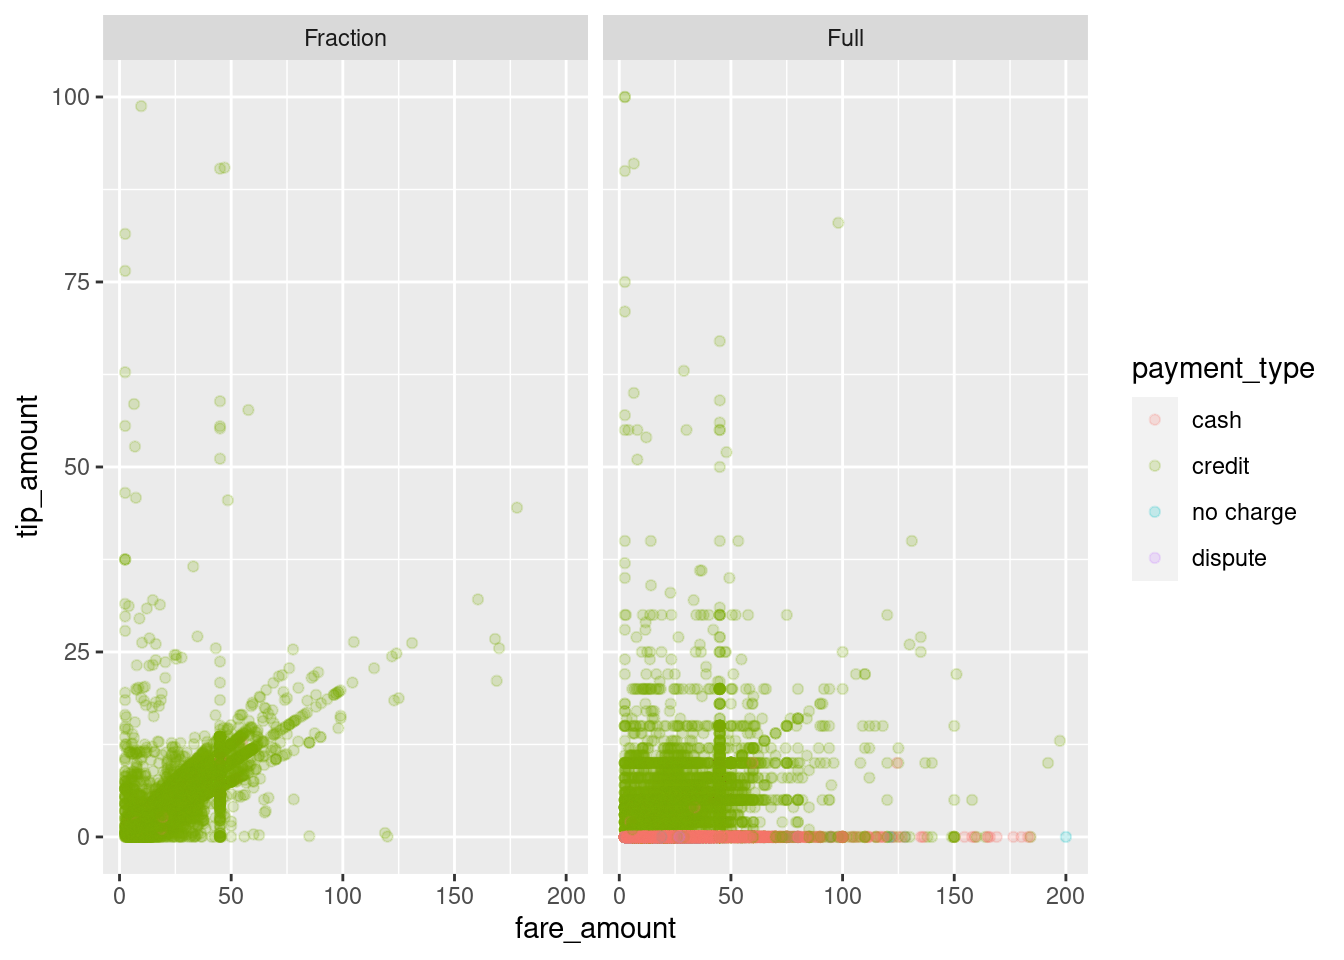
\includegraphics{bigdata_files/figure-latex/unnamed-chunk-132-1.pdf}

Now the picture is getting clearer. Paying tip seems to follow certain rules of thumb. Certain fixed amounts tend to be paid independent of the fare amount (visible in the straight lines of dots on the right-hand panel). At the same time, the pattern in the left panel indicates another habit: computing the amount of tip as a linear function of the total fare amount (`pay 10\% tip'). A third habit might be to determine the amount of tip by `rounding up' the total amount paid. In the following, we try to tease the latter out, only focusing on credit card payments.

\begin{Shaded}
\begin{Highlighting}[]
\NormalTok{taxi[, rounded\_up }\SpecialCharTok{:}\ErrorTok{=} \FunctionTok{ifelse}\NormalTok{(fare\_amount }\SpecialCharTok{+}\NormalTok{ tip\_amount }\SpecialCharTok{==} \FunctionTok{round}\NormalTok{(fare\_amount }\SpecialCharTok{+}\NormalTok{ tip\_amount, }\DecValTok{0}\NormalTok{),}
                            \StringTok{"Rounded up"}\NormalTok{,}
                            \StringTok{"Not rounded"}\NormalTok{)]}
\CommentTok{\# extended x/y plot}
\NormalTok{taxiplot }\SpecialCharTok{+}
     \FunctionTok{geom\_point}\NormalTok{(}\AttributeTok{data=}\NormalTok{ taxi[payment\_type }\SpecialCharTok{==} \StringTok{"credit"}\NormalTok{],}
                \AttributeTok{alpha=}\FloatTok{0.2}\NormalTok{, }\FunctionTok{aes}\NormalTok{(}\AttributeTok{color=}\NormalTok{rounded\_up)) }\SpecialCharTok{+}
     \FunctionTok{facet\_wrap}\NormalTok{(}\StringTok{"dollar\_paid"}\NormalTok{)}
\end{Highlighting}
\end{Shaded}

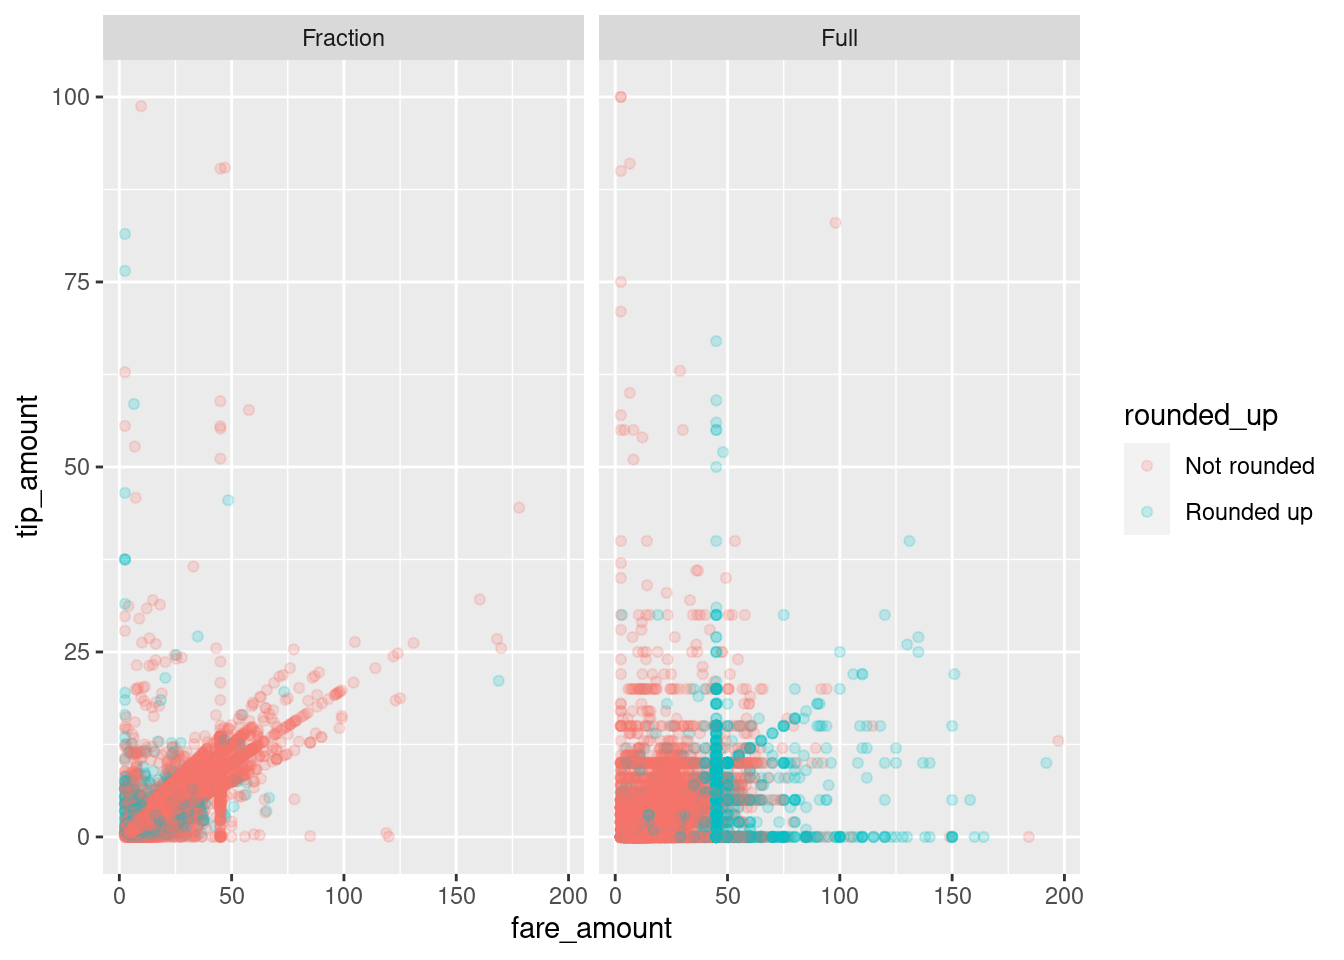
\includegraphics{bigdata_files/figure-latex/unnamed-chunk-133-1.pdf}

Now we can start modelling. A reasonable first shot is to model the tip amount as a linear function of the fare amount, conditional on the no-zero tip amounts paid as fractions of a dollar.

\begin{Shaded}
\begin{Highlighting}[]
\NormalTok{modelplot }\OtherTok{\textless{}{-}} \FunctionTok{ggplot}\NormalTok{(}\AttributeTok{data=}\NormalTok{ taxi[payment\_type }\SpecialCharTok{==} \StringTok{"credit"} \SpecialCharTok{\&}\NormalTok{ dollar\_paid }\SpecialCharTok{==} \StringTok{"Fraction"} \SpecialCharTok{\&} \DecValTok{0} \SpecialCharTok{\textless{}}\NormalTok{ tip\_amount],}
                    \FunctionTok{aes}\NormalTok{(}\AttributeTok{x =}\NormalTok{ fare\_amount, }\AttributeTok{y =}\NormalTok{ tip\_amount))}
\NormalTok{modelplot }\SpecialCharTok{+}
     \FunctionTok{geom\_point}\NormalTok{(}\AttributeTok{alpha=}\FloatTok{0.2}\NormalTok{, }\AttributeTok{colour=}\StringTok{"darkgreen"}\NormalTok{) }\SpecialCharTok{+}
     \FunctionTok{geom\_smooth}\NormalTok{(}\AttributeTok{method =} \StringTok{"lm"}\NormalTok{, }\AttributeTok{colour =} \StringTok{"black"}\NormalTok{)}
\end{Highlighting}
\end{Shaded}

\begin{verbatim}
## `geom_smooth()` using formula 'y ~ x'
\end{verbatim}

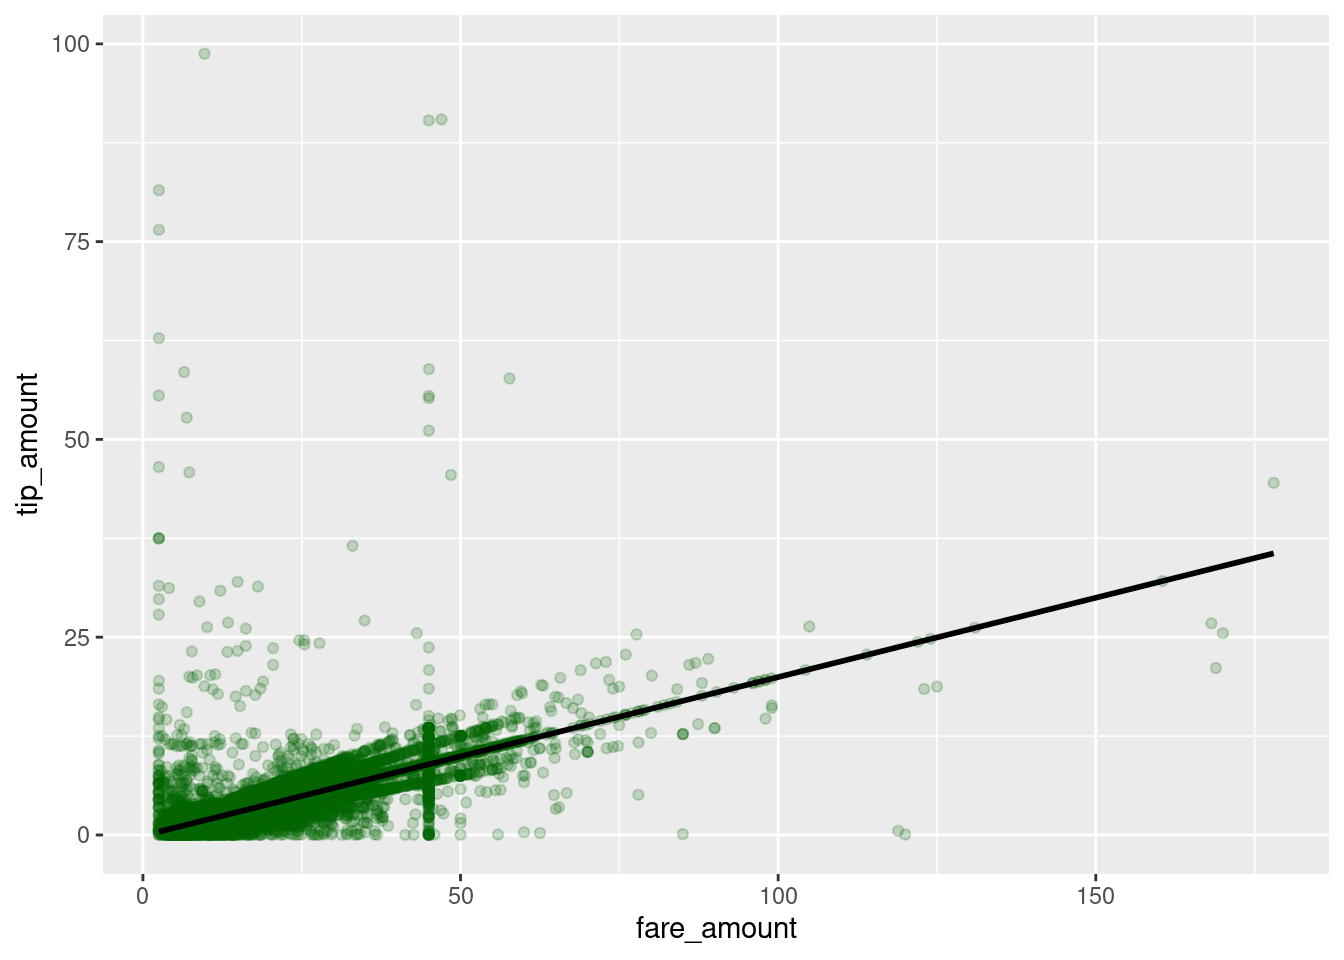
\includegraphics{bigdata_files/figure-latex/unnamed-chunk-134-1.pdf}

Finally, we prepare the plot for reporting. \texttt{ggplot2} provides several predefined `themes' for plots which define all kind of aspects of a plot (background color, line colors, font size etc.). The easiest way to tweak the design of your final plot in a certain direction is to just add such a pre-defined theme at the end of your plot. Some of the pre-defined themes allow you to change a few aspects such as the font type and the base size of all the texts in the plot (labels and tick numbers etc.). Here, we use the \texttt{theme\_bw()}, increase the font size and switch to serif-type font. \texttt{theme\_bw()} is one of the complete themes already shipped with the basic \texttt{ggplot2} installation.\footnote{See \href{https://ggplot2.tidyverse.org/reference/ggtheme.html}{the ggplot2 documentation} for a list of all pre-defined themes shipped with the basic installation.} Many more themes can be found in additional R packages (see, for example, the \href{https://cran.r-project.org/web/packages/ggthemes/index.html}{\texttt{ggthemes} package}).

\begin{Shaded}
\begin{Highlighting}[]
\NormalTok{modelplot }\OtherTok{\textless{}{-}} \FunctionTok{ggplot}\NormalTok{(}\AttributeTok{data=}\NormalTok{ taxi[payment\_type }\SpecialCharTok{==} \StringTok{"credit"} \SpecialCharTok{\&}\NormalTok{ dollar\_paid }\SpecialCharTok{==} \StringTok{"Fraction"} \SpecialCharTok{\&} \DecValTok{0} \SpecialCharTok{\textless{}}\NormalTok{ tip\_amount],}
                    \FunctionTok{aes}\NormalTok{(}\AttributeTok{x =}\NormalTok{ fare\_amount, }\AttributeTok{y =}\NormalTok{ tip\_amount))}
\NormalTok{modelplot }\SpecialCharTok{+}
     \FunctionTok{geom\_point}\NormalTok{(}\AttributeTok{alpha=}\FloatTok{0.2}\NormalTok{, }\AttributeTok{colour=}\StringTok{"darkgreen"}\NormalTok{) }\SpecialCharTok{+}
     \FunctionTok{geom\_smooth}\NormalTok{(}\AttributeTok{method =} \StringTok{"lm"}\NormalTok{, }\AttributeTok{colour =} \StringTok{"black"}\NormalTok{) }\SpecialCharTok{+}
     \FunctionTok{ylab}\NormalTok{(}\StringTok{"Amount of tip paid (in USD)"}\NormalTok{) }\SpecialCharTok{+}
     \FunctionTok{xlab}\NormalTok{(}\StringTok{"Amount of fare paid (in USD)"}\NormalTok{) }\SpecialCharTok{+}
     \FunctionTok{theme\_bw}\NormalTok{(}\AttributeTok{base\_size =} \DecValTok{18}\NormalTok{, }\AttributeTok{base\_family =} \StringTok{"serif"}\NormalTok{)}
\end{Highlighting}
\end{Shaded}

\begin{verbatim}
## `geom_smooth()` using formula 'y ~ x'
\end{verbatim}

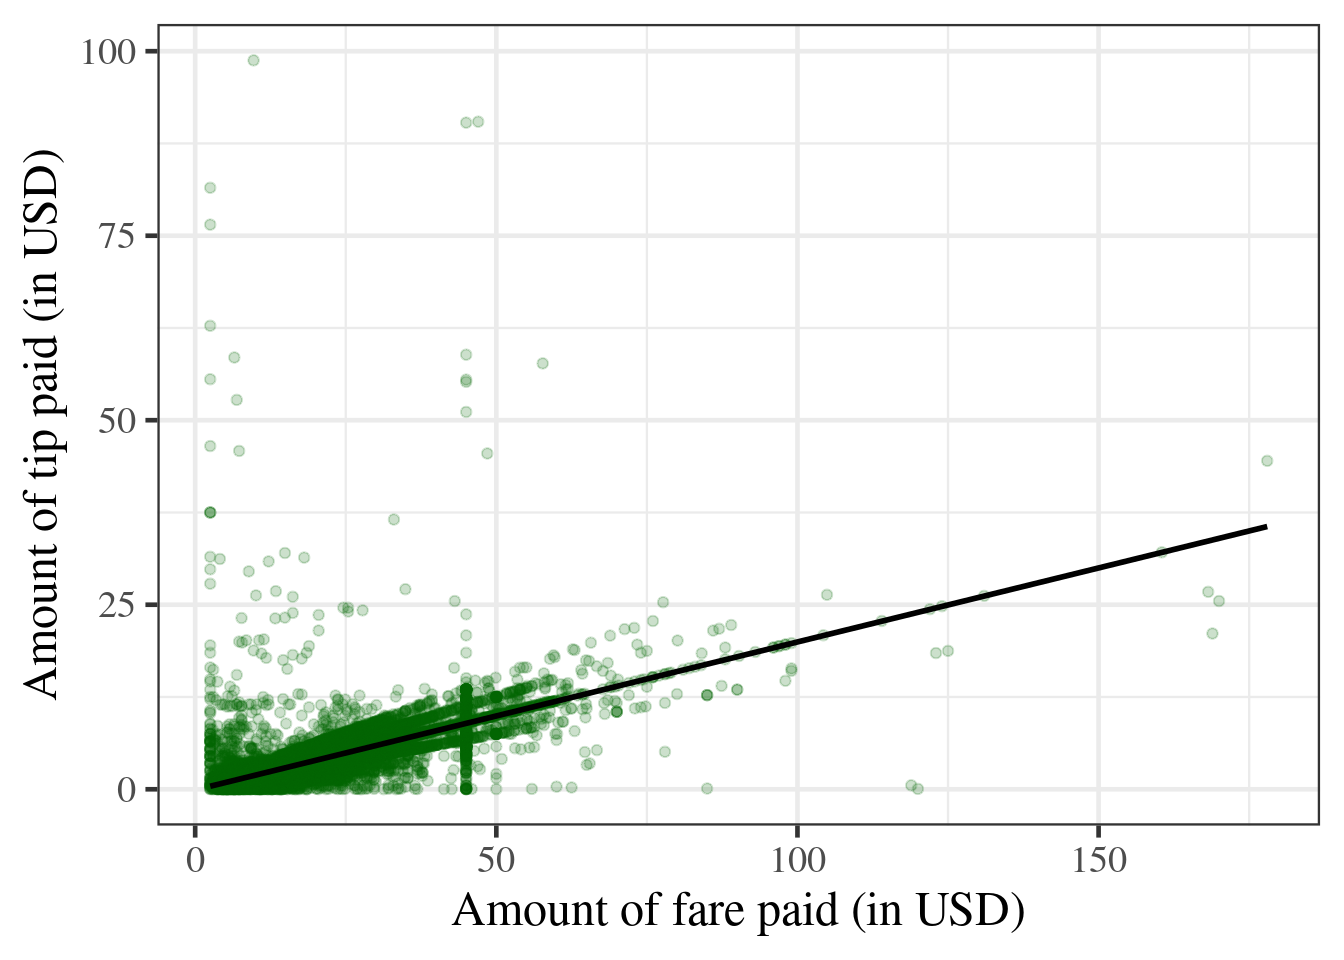
\includegraphics{bigdata_files/figure-latex/unnamed-chunk-135-1.pdf}

\hypertarget{excursus-modify-and-create-themes}{%
\section{Excursus: modify and create themes}\label{excursus-modify-and-create-themes}}

Apart from using pre-defined themes as illustrated above, we can use the \texttt{theme()} function to further modify the design of a plot. For example, we can print the axis labels (`axis titles') in bold.

\begin{Shaded}
\begin{Highlighting}[]
\NormalTok{modelplot }\OtherTok{\textless{}{-}} \FunctionTok{ggplot}\NormalTok{(}\AttributeTok{data=}\NormalTok{ taxi[payment\_type }\SpecialCharTok{==} \StringTok{"credit"} \SpecialCharTok{\&}\NormalTok{ dollar\_paid }\SpecialCharTok{==} \StringTok{"Fraction"} \SpecialCharTok{\&} \DecValTok{0} \SpecialCharTok{\textless{}}\NormalTok{ tip\_amount],}
                    \FunctionTok{aes}\NormalTok{(}\AttributeTok{x =}\NormalTok{ fare\_amount, }\AttributeTok{y =}\NormalTok{ tip\_amount))}
\NormalTok{modelplot }\SpecialCharTok{+}
     \FunctionTok{geom\_point}\NormalTok{(}\AttributeTok{alpha=}\FloatTok{0.2}\NormalTok{, }\AttributeTok{colour=}\StringTok{"darkgreen"}\NormalTok{) }\SpecialCharTok{+}
     \FunctionTok{geom\_smooth}\NormalTok{(}\AttributeTok{method =} \StringTok{"lm"}\NormalTok{, }\AttributeTok{colour =} \StringTok{"black"}\NormalTok{) }\SpecialCharTok{+}
     \FunctionTok{ylab}\NormalTok{(}\StringTok{"Amount of tip paid (in USD)"}\NormalTok{) }\SpecialCharTok{+}
     \FunctionTok{xlab}\NormalTok{(}\StringTok{"Amount of fare paid (in USD)"}\NormalTok{) }\SpecialCharTok{+}
     \FunctionTok{theme\_bw}\NormalTok{(}\AttributeTok{base\_size =} \DecValTok{18}\NormalTok{, }\AttributeTok{base\_family =} \StringTok{"serif"}\NormalTok{) }\SpecialCharTok{+}
     \FunctionTok{theme}\NormalTok{(}\AttributeTok{axis.title =} \FunctionTok{element\_text}\NormalTok{(}\AttributeTok{face=}\StringTok{"bold"}\NormalTok{))}
\end{Highlighting}
\end{Shaded}

\begin{verbatim}
## `geom_smooth()` using formula 'y ~ x'
\end{verbatim}

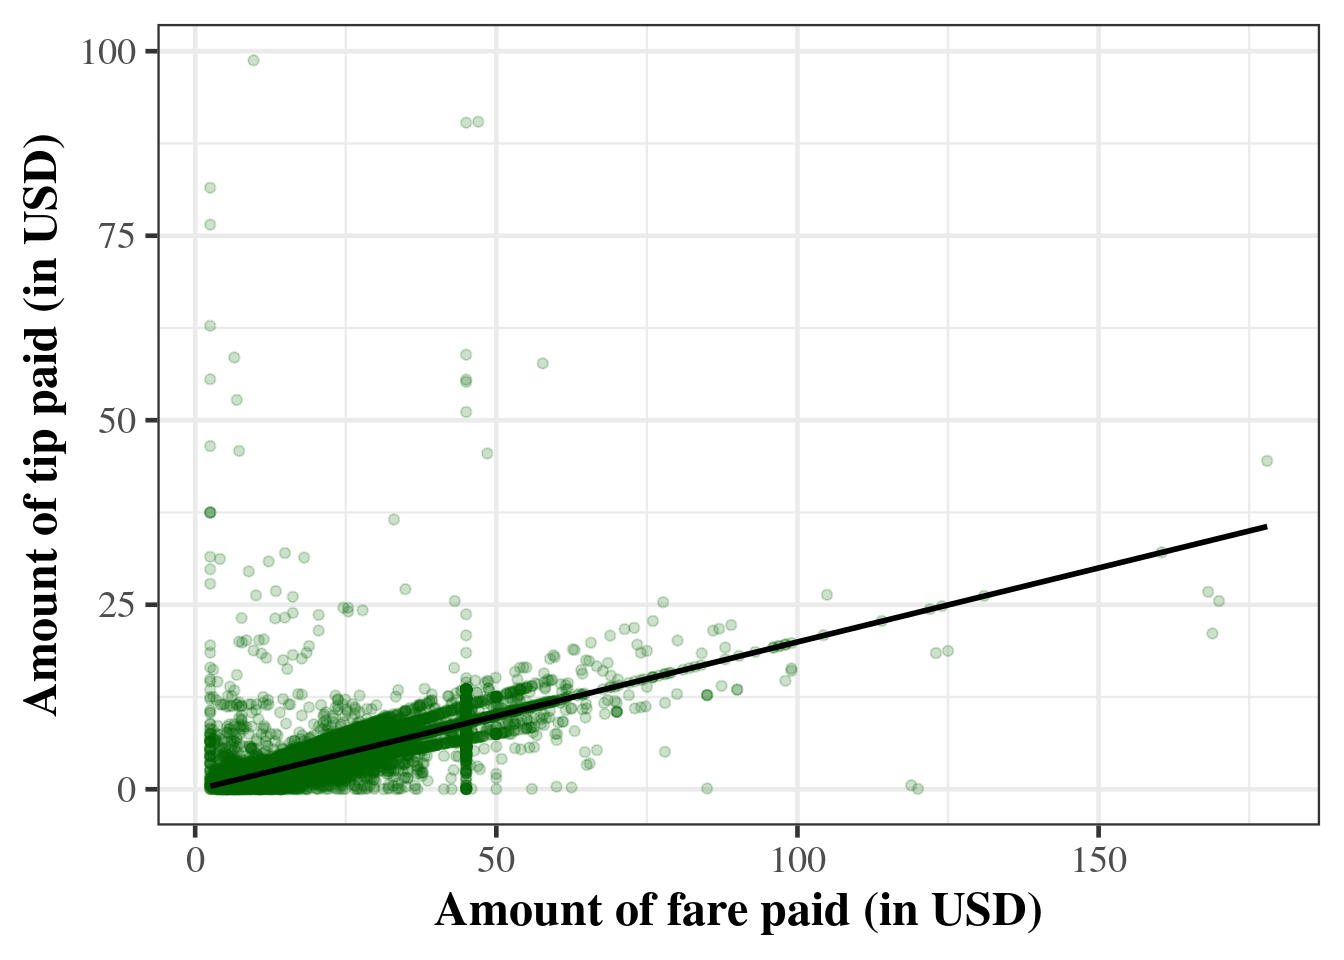
\includegraphics{bigdata_files/figure-latex/unnamed-chunk-136-1.pdf}

There is a large list of plot design aspects that can be modified in this way (see \texttt{?theme()} for details).

\hypertarget{create-your-own-theme-simple-approach}{%
\subsection{Create your own theme: simple approach}\label{create-your-own-theme-simple-approach}}

Extensive design modifications via \texttt{theme()} can involve many lines of code, making your plot code harder to read/understand. In practice, you might want to define your specific theme once and then apply this theme to all of your plots. In order to do so it makes sense to choose one of the existing themes as a basis and then modify its design aspects until you have the design you are looking for. Following the design choices in the examples above, we can create our own \texttt{theme\_my\_serif()} as follows.

\begin{Shaded}
\begin{Highlighting}[]
\CommentTok{\# \textquotesingle{}define\textquotesingle{} a new theme}
\NormalTok{theme\_my\_serif }\OtherTok{\textless{}{-}}      
  \FunctionTok{theme\_bw}\NormalTok{(}\AttributeTok{base\_size =} \DecValTok{18}\NormalTok{, }\AttributeTok{base\_family =} \StringTok{"serif"}\NormalTok{) }\SpecialCharTok{+}
  \FunctionTok{theme}\NormalTok{(}\AttributeTok{axis.title =} \FunctionTok{element\_text}\NormalTok{(}\AttributeTok{face=}\StringTok{"bold"}\NormalTok{))}

\CommentTok{\# apply it }
\NormalTok{modelplot }\SpecialCharTok{+}
     \FunctionTok{geom\_point}\NormalTok{(}\AttributeTok{alpha=}\FloatTok{0.2}\NormalTok{, }\AttributeTok{colour=}\StringTok{"darkgreen"}\NormalTok{) }\SpecialCharTok{+}
     \FunctionTok{geom\_smooth}\NormalTok{(}\AttributeTok{method =} \StringTok{"lm"}\NormalTok{, }\AttributeTok{colour =} \StringTok{"black"}\NormalTok{) }\SpecialCharTok{+}
     \FunctionTok{ylab}\NormalTok{(}\StringTok{"Amount of tip paid (in USD)"}\NormalTok{) }\SpecialCharTok{+}
     \FunctionTok{xlab}\NormalTok{(}\StringTok{"Amount of fare paid (in USD)"}\NormalTok{) }\SpecialCharTok{+}
\NormalTok{  theme\_my\_serif}
\end{Highlighting}
\end{Shaded}

\begin{verbatim}
## `geom_smooth()` using formula 'y ~ x'
\end{verbatim}

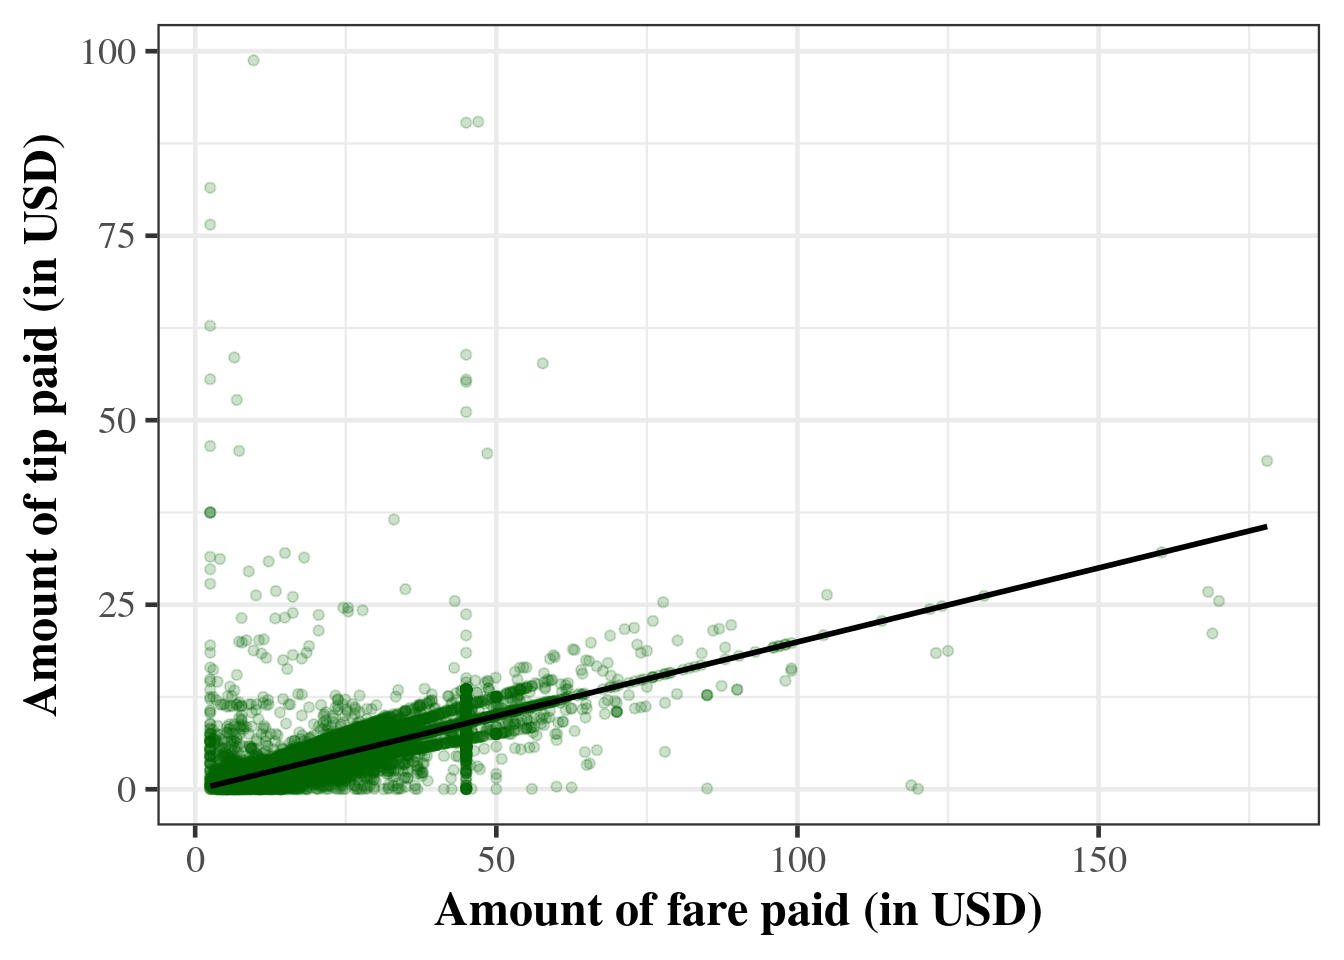
\includegraphics{bigdata_files/figure-latex/unnamed-chunk-137-1.pdf}

This practical approach does not require you to define every aspect of a theme. If you indeed want completely define every aspect of a theme, you can set \texttt{complete=TRUE} when calling the theme function.

\begin{Shaded}
\begin{Highlighting}[]
\CommentTok{\# \textquotesingle{}define\textquotesingle{} a new theme}
\NormalTok{my\_serif\_theme }\OtherTok{\textless{}{-}}      
  \FunctionTok{theme\_bw}\NormalTok{(}\AttributeTok{base\_size =} \DecValTok{18}\NormalTok{, }\AttributeTok{base\_family =} \StringTok{"serif"}\NormalTok{) }\SpecialCharTok{+}
  \FunctionTok{theme}\NormalTok{(}\AttributeTok{axis.title =} \FunctionTok{element\_text}\NormalTok{(}\AttributeTok{face=}\StringTok{"bold"}\NormalTok{), }\AttributeTok{complete =} \ConstantTok{TRUE}\NormalTok{)}

\CommentTok{\# apply it }
\NormalTok{modelplot }\SpecialCharTok{+}
     \FunctionTok{geom\_point}\NormalTok{(}\AttributeTok{alpha=}\FloatTok{0.2}\NormalTok{, }\AttributeTok{colour=}\StringTok{"darkgreen"}\NormalTok{) }\SpecialCharTok{+}
     \FunctionTok{geom\_smooth}\NormalTok{(}\AttributeTok{method =} \StringTok{"lm"}\NormalTok{, }\AttributeTok{colour =} \StringTok{"black"}\NormalTok{) }\SpecialCharTok{+}
     \FunctionTok{ylab}\NormalTok{(}\StringTok{"Amount of tip paid (in USD)"}\NormalTok{) }\SpecialCharTok{+}
     \FunctionTok{xlab}\NormalTok{(}\StringTok{"Amount of fare paid (in USD)"}\NormalTok{) }\SpecialCharTok{+}
\NormalTok{  theme\_my\_serif}
\end{Highlighting}
\end{Shaded}

\begin{verbatim}
## `geom_smooth()` using formula 'y ~ x'
\end{verbatim}

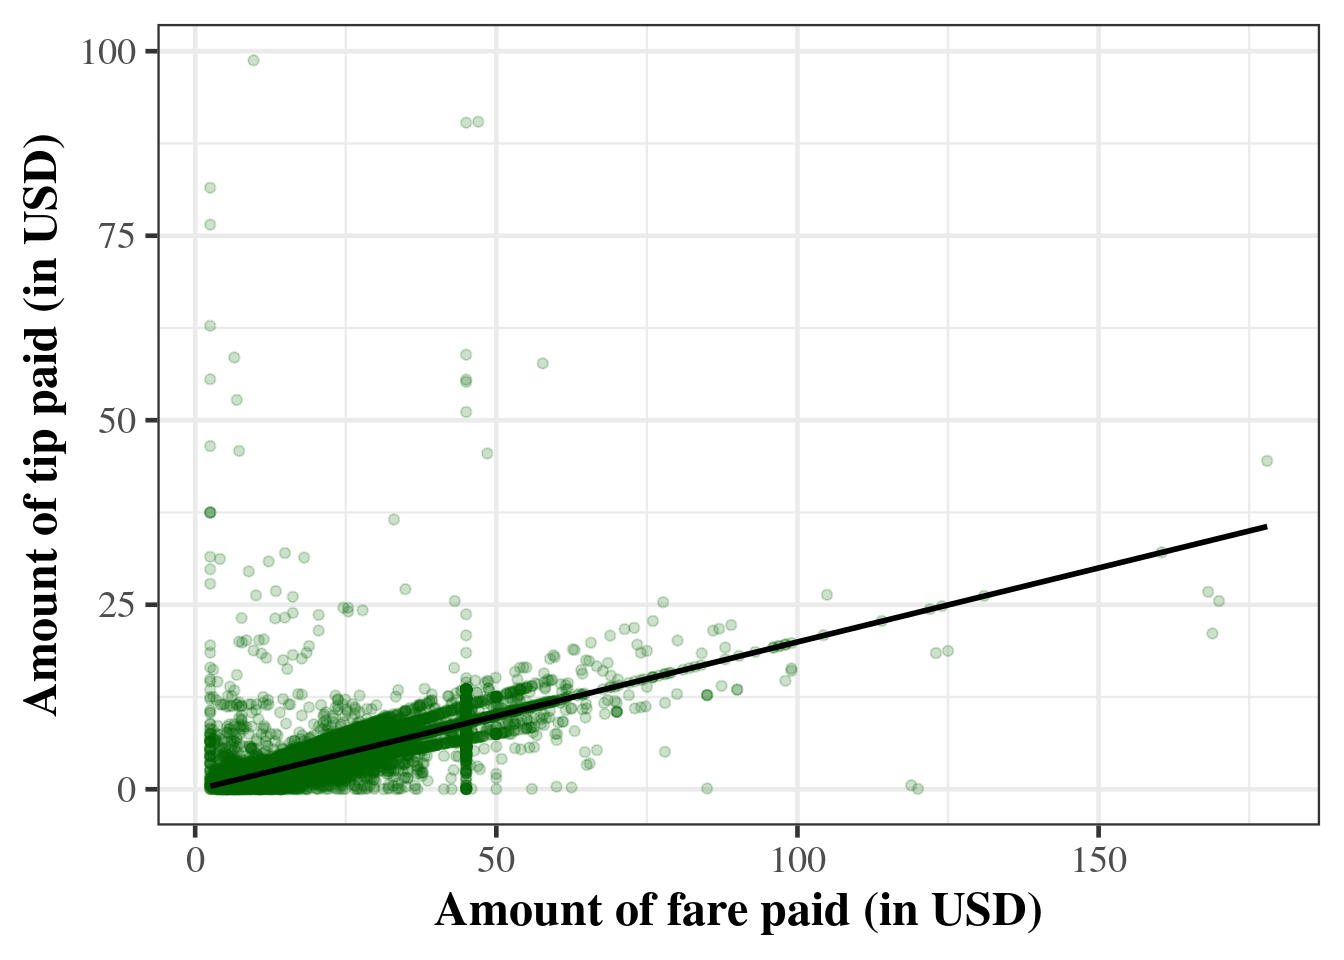
\includegraphics{bigdata_files/figure-latex/unnamed-chunk-138-1.pdf}

Note that since we have only defined one aspect (bold axis titles), the rest of the elements follow the default theme.

Importantly, the approach outlined above does technically not really create a new theme like \texttt{theme\_bw()}, as these pre-defined themes are implemented as functions. Note that we add the new theme simply with \texttt{+\ theme\_my\_serif} to the plot (no parentheses). In practice this is the most simple approach and it provides all the functionality you need in order to apply your own `theme' to each of your plots.

\hypertarget{implementing-actual-themes-as-functions.}{%
\subsection{Implementing actual themes as functions.}\label{implementing-actual-themes-as-functions.}}

If you really want to implement a theme as a function. The following blueprint can get you started.

\begin{Shaded}
\begin{Highlighting}[]
\CommentTok{\# define own theme}
\NormalTok{theme\_my\_serif }\OtherTok{\textless{}{-}} 
  \ControlFlowTok{function}\NormalTok{(}\AttributeTok{base\_size =} \DecValTok{15}\NormalTok{,}
           \AttributeTok{base\_family =} \StringTok{""}\NormalTok{,}
           \AttributeTok{base\_line\_size =}\NormalTok{ base\_size}\SpecialCharTok{/}\DecValTok{170}\NormalTok{,}
           \AttributeTok{base\_rect\_size =}\NormalTok{ base\_size}\SpecialCharTok{/}\DecValTok{170}\NormalTok{)\{ }
    
    \FunctionTok{theme\_bw}\NormalTok{(}\AttributeTok{base\_size =}\NormalTok{ base\_size,}
             \AttributeTok{base\_family =}\NormalTok{ base\_family,}
             \AttributeTok{base\_line\_size =}\NormalTok{ base\_size}\SpecialCharTok{/}\DecValTok{170}\NormalTok{,}
             \AttributeTok{base\_rect\_size =}\NormalTok{ base\_size}\SpecialCharTok{/}\DecValTok{170}\NormalTok{) }\SpecialCharTok{\%+replace\%}    \CommentTok{\# use theme\_bw() as a basis but replace some design elements}
    \FunctionTok{theme}\NormalTok{(}
      \AttributeTok{axis.title =} \FunctionTok{element\_text}\NormalTok{(}\AttributeTok{face=}\StringTok{"bold"}\NormalTok{)}
\NormalTok{    )}
\NormalTok{  \}}

\CommentTok{\# apply the theme}
\CommentTok{\# apply it }
\NormalTok{modelplot }\SpecialCharTok{+}
     \FunctionTok{geom\_point}\NormalTok{(}\AttributeTok{alpha=}\FloatTok{0.2}\NormalTok{, }\AttributeTok{colour=}\StringTok{"darkgreen"}\NormalTok{) }\SpecialCharTok{+}
     \FunctionTok{geom\_smooth}\NormalTok{(}\AttributeTok{method =} \StringTok{"lm"}\NormalTok{, }\AttributeTok{colour =} \StringTok{"black"}\NormalTok{) }\SpecialCharTok{+}
     \FunctionTok{ylab}\NormalTok{(}\StringTok{"Amount of tip paid (in USD)"}\NormalTok{) }\SpecialCharTok{+}
     \FunctionTok{xlab}\NormalTok{(}\StringTok{"Amount of fare paid (in USD)"}\NormalTok{) }\SpecialCharTok{+}
  \FunctionTok{theme\_my\_serif}\NormalTok{(}\AttributeTok{base\_size =} \DecValTok{18}\NormalTok{, }\AttributeTok{base\_family=}\StringTok{"serif"}\NormalTok{)}
\end{Highlighting}
\end{Shaded}

\begin{verbatim}
## `geom_smooth()` using formula 'y ~ x'
\end{verbatim}

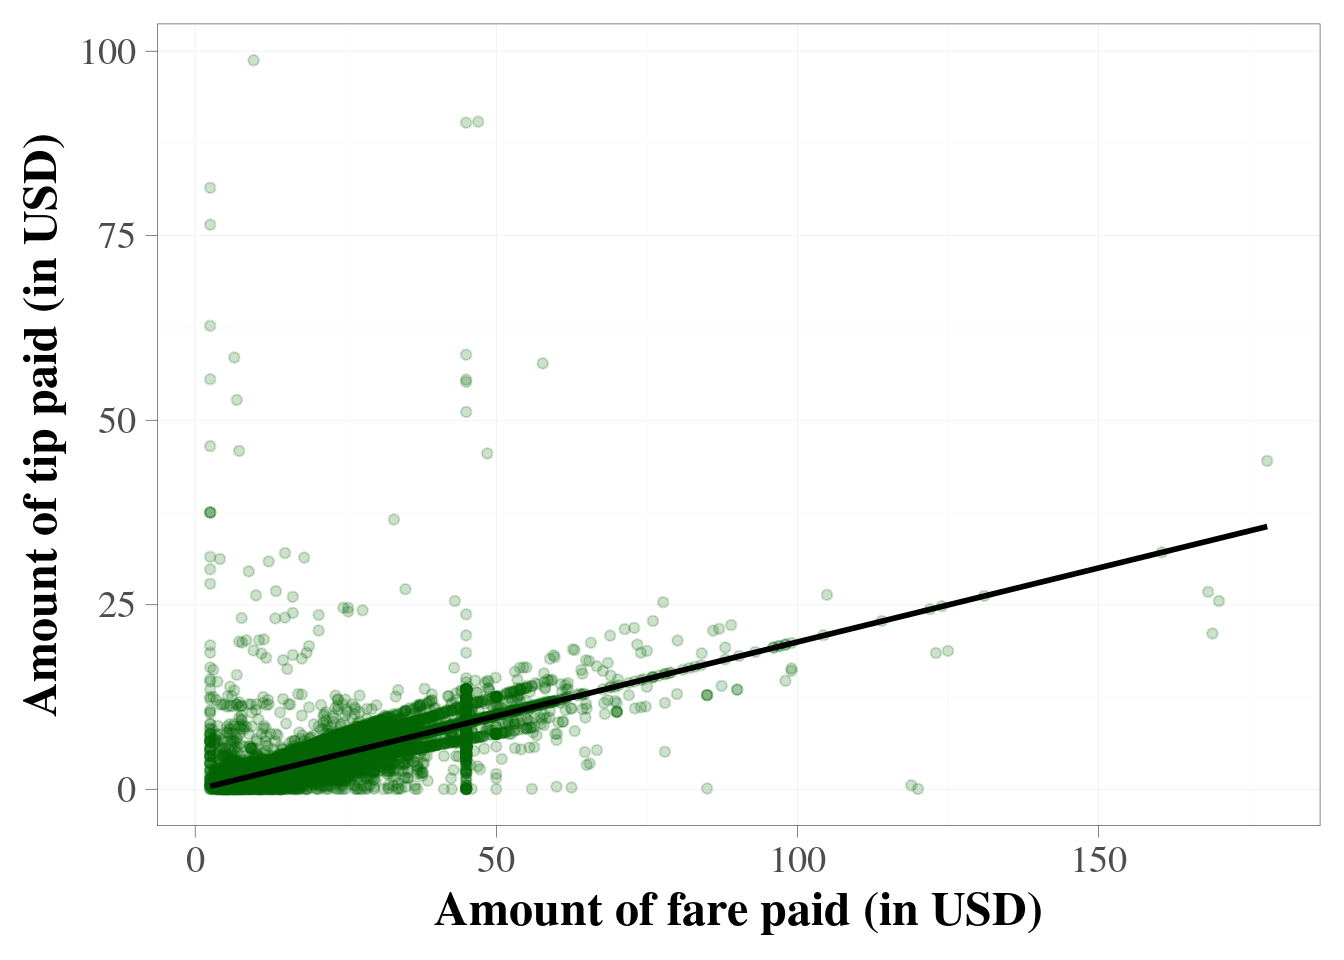
\includegraphics{bigdata_files/figure-latex/unnamed-chunk-139-1.pdf}

\hypertarget{visualize-time-and-space}{%
\section{Visualize Time and Space}\label{visualize-time-and-space}}

The previous visualization exercises were focused on visually exploring patterns in the tipping behavior of people taking a NYC yellow cap ride. Based on the same data set, will explore the time dimension and spatial dimension of the TLC Yellow Cap data. That is, we explore where trips tend to start and end, depending on the time of the day.

\hypertarget{preparations}{%
\subsection{Preparations}\label{preparations}}

For the visualization of spatial data we first load additional packages that give R some \href{https://en.wikipedia.org/wiki/Geographic_information_system}{GIS} features.

\begin{Shaded}
\begin{Highlighting}[]
\CommentTok{\# load GIS packages}
\FunctionTok{library}\NormalTok{(rgdal)}
\FunctionTok{library}\NormalTok{(rgeos)}
\end{Highlighting}
\end{Shaded}

Moreover, we download and import a so-called \href{https://en.wikipedia.org/wiki/Shapefile}{`shape file'} (a geospatial data format) of New York City. This will be the basis for our visualization of the spatial dimension of taxi trips. The file is downloaded from \href{https://www1.nyc.gov/site/planning/index.page}{New York's Department of City Planning} and indicates the city's community district borders.\footnote{Similar files are provided online by most city authorities in developed countries. See, for example, GIS Data for the City and Canton of Zurich: \url{https://maps.zh.ch/}.}

\begin{Shaded}
\begin{Highlighting}[]
\CommentTok{\# download the zipped shapefile to a temporary file, unzip}
\NormalTok{URL }\OtherTok{\textless{}{-}} \StringTok{"https://www1.nyc.gov/assets/planning/download/zip/data{-}maps/open{-}data/nycd\_19a.zip"}
\NormalTok{tmp\_file }\OtherTok{\textless{}{-}} \FunctionTok{tempfile}\NormalTok{()}
\FunctionTok{download.file}\NormalTok{(URL, tmp\_file)}
\NormalTok{file\_path }\OtherTok{\textless{}{-}} \FunctionTok{unzip}\NormalTok{(tmp\_file, }\AttributeTok{exdir=} \StringTok{"data"}\NormalTok{)}
\CommentTok{\# delete the temporary file}
\FunctionTok{unlink}\NormalTok{(tmp\_file)}
\end{Highlighting}
\end{Shaded}

Now we can import the shape file and have a look at how the GIS data is structured.

\begin{Shaded}
\begin{Highlighting}[]
\CommentTok{\# read GIS data}
\NormalTok{nyc\_map }\OtherTok{\textless{}{-}} \FunctionTok{readOGR}\NormalTok{(file\_path[}\DecValTok{1}\NormalTok{], }\AttributeTok{verbose =} \ConstantTok{FALSE}\NormalTok{)}

\CommentTok{\# have a look at the GIS data}
\FunctionTok{summary}\NormalTok{(nyc\_map)}
\end{Highlighting}
\end{Shaded}

\begin{verbatim}
## Object of class SpatialPolygonsDataFrame
## Coordinates:
##      min     max
## x 913175 1067383
## y 120122  272844
## Is projected: TRUE 
## proj4string :
## [+proj=lcc +lat_0=40.1666666666667 +lon_0=-74
## +lat_1=41.0333333333333 +lat_2=40.6666666666667
## +x_0=300000 +y_0=0 +datum=NAD83 +units=us-ft
## +no_defs]
## Data attributes:
##      BoroCD      Shape_Leng       Shape_Area      
##  Min.   :101   Min.   : 23963   Min.   :2.43e+07  
##  1st Qu.:206   1st Qu.: 36611   1st Qu.:4.84e+07  
##  Median :308   Median : 52246   Median :8.27e+07  
##  Mean   :297   Mean   : 74890   Mean   :1.19e+08  
##  3rd Qu.:406   3rd Qu.: 85711   3rd Qu.:1.37e+08  
##  Max.   :595   Max.   :270660   Max.   :5.99e+08
\end{verbatim}

Note that the coordinates are not in the usual longitude and latitude units. The original map uses a different projection than the TLC data of cap trips records. Before plotting, we thus have to change the projection to be in line with the TLC data.

\begin{Shaded}
\begin{Highlighting}[]
\CommentTok{\# transform the projection}
\NormalTok{nyc\_map }\OtherTok{\textless{}{-}} \FunctionTok{spTransform}\NormalTok{(nyc\_map, }\FunctionTok{CRS}\NormalTok{(}\StringTok{"+proj=longlat +datum=WGS84 +no\_defs +ellps=WGS84 +towgs84=0,0,0"}\NormalTok{))}
\CommentTok{\# check result}
\FunctionTok{summary}\NormalTok{(nyc\_map)}
\end{Highlighting}
\end{Shaded}

\begin{verbatim}
## Object of class SpatialPolygonsDataFrame
## Coordinates:
##      min    max
## x -74.26 -73.70
## y  40.50  40.92
## Is projected: FALSE 
## proj4string : [+proj=longlat +datum=WGS84 +no_defs]
## Data attributes:
##      BoroCD      Shape_Leng       Shape_Area      
##  Min.   :101   Min.   : 23963   Min.   :2.43e+07  
##  1st Qu.:206   1st Qu.: 36611   1st Qu.:4.84e+07  
##  Median :308   Median : 52246   Median :8.27e+07  
##  Mean   :297   Mean   : 74890   Mean   :1.19e+08  
##  3rd Qu.:406   3rd Qu.: 85711   3rd Qu.:1.37e+08  
##  Max.   :595   Max.   :270660   Max.   :5.99e+08
\end{verbatim}

One last preparatory step is to convert the map data to a \texttt{data.frame} for plotting with \texttt{ggplot}.

\begin{Shaded}
\begin{Highlighting}[]
\NormalTok{nyc\_map }\OtherTok{\textless{}{-}} \FunctionTok{fortify}\NormalTok{(nyc\_map)}
\end{Highlighting}
\end{Shaded}

\hypertarget{pick-up-and-drop-off-locations}{%
\subsection{Pick-up and drop-off locations}\label{pick-up-and-drop-off-locations}}

Since trips might actually start or end outside of NYC, we first restrict the sample of trips to those within the boundary box of the map. For the sake of the exercise, we only select a random sample of \texttt{50000} trips from the remaining trip records.

\begin{Shaded}
\begin{Highlighting}[]
\CommentTok{\# taxi trips plot data}
\NormalTok{taxi\_trips }\OtherTok{\textless{}{-}}\NormalTok{ taxi[start\_long }\SpecialCharTok{\textless{}=} \FunctionTok{max}\NormalTok{(nyc\_map}\SpecialCharTok{$}\NormalTok{long) }\SpecialCharTok{\&} 
\NormalTok{                        start\_long }\SpecialCharTok{\textgreater{}=} \FunctionTok{min}\NormalTok{(nyc\_map}\SpecialCharTok{$}\NormalTok{long) }\SpecialCharTok{\&}
\NormalTok{                        dest\_long }\SpecialCharTok{\textless{}=} \FunctionTok{max}\NormalTok{(nyc\_map}\SpecialCharTok{$}\NormalTok{long) }\SpecialCharTok{\&}
\NormalTok{                        dest\_long }\SpecialCharTok{\textgreater{}=} \FunctionTok{min}\NormalTok{(nyc\_map}\SpecialCharTok{$}\NormalTok{long) }\SpecialCharTok{\&}
\NormalTok{                        start\_lat }\SpecialCharTok{\textless{}=} \FunctionTok{max}\NormalTok{(nyc\_map}\SpecialCharTok{$}\NormalTok{lat) }\SpecialCharTok{\&} 
\NormalTok{                        start\_lat }\SpecialCharTok{\textgreater{}=} \FunctionTok{min}\NormalTok{(nyc\_map}\SpecialCharTok{$}\NormalTok{lat) }\SpecialCharTok{\&}
\NormalTok{                        dest\_lat }\SpecialCharTok{\textless{}=} \FunctionTok{max}\NormalTok{(nyc\_map}\SpecialCharTok{$}\NormalTok{lat) }\SpecialCharTok{\&}
\NormalTok{                        dest\_lat }\SpecialCharTok{\textgreater{}=} \FunctionTok{min}\NormalTok{(nyc\_map}\SpecialCharTok{$}\NormalTok{lat) }
\NormalTok{                        ]}
\NormalTok{taxi\_trips }\OtherTok{\textless{}{-}}\NormalTok{ taxi\_trips[}\FunctionTok{sample}\NormalTok{(}\FunctionTok{nrow}\NormalTok{(taxi\_trips), }\DecValTok{50000}\NormalTok{)]}
\end{Highlighting}
\end{Shaded}

In order to visualize how the cap traffic is changing over the course of the day, we add an additional variable called \texttt{start\_time} in which we store the time (hour) of the day a trip started.

\begin{Shaded}
\begin{Highlighting}[]
\NormalTok{taxi\_trips}\SpecialCharTok{$}\NormalTok{start\_time }\OtherTok{\textless{}{-}} \FunctionTok{hour}\NormalTok{(taxi\_trips}\SpecialCharTok{$}\NormalTok{pickup\_time)}
\end{Highlighting}
\end{Shaded}

Particularly, we want to look at differences between, morning, afternoon, and evening/night.

\begin{Shaded}
\begin{Highlighting}[]
\CommentTok{\# define new variable for facets}
\NormalTok{taxi\_trips}\SpecialCharTok{$}\NormalTok{time\_of\_day }\OtherTok{\textless{}{-}} \StringTok{"Morning"}
\NormalTok{taxi\_trips[start\_time }\SpecialCharTok{\textgreater{}} \DecValTok{12} \SpecialCharTok{\&}\NormalTok{ start\_time }\SpecialCharTok{\textless{}} \DecValTok{17}\NormalTok{]}\SpecialCharTok{$}\NormalTok{time\_of\_day }\OtherTok{\textless{}{-}} \StringTok{"Afternoon"}
\NormalTok{taxi\_trips[start\_time }\SpecialCharTok{\%in\%} \FunctionTok{c}\NormalTok{(}\DecValTok{17}\SpecialCharTok{:}\DecValTok{24}\NormalTok{, }\DecValTok{0}\SpecialCharTok{:}\DecValTok{5}\NormalTok{)]}\SpecialCharTok{$}\NormalTok{time\_of\_day }\OtherTok{\textless{}{-}} \StringTok{"Evening/Night"}
\NormalTok{taxi\_trips}\SpecialCharTok{$}\NormalTok{time\_of\_day  }\OtherTok{\textless{}{-}} \FunctionTok{factor}\NormalTok{(taxi\_trips}\SpecialCharTok{$}\NormalTok{time\_of\_day, }\AttributeTok{levels =} \FunctionTok{c}\NormalTok{(}\StringTok{"Morning"}\NormalTok{, }\StringTok{"Afternoon"}\NormalTok{, }\StringTok{"Evening/Night"}\NormalTok{))}
\end{Highlighting}
\end{Shaded}

We initiate the plot by first setting up the canvas with our taxi trips data. Then, we add the map as a first layer.

\begin{Shaded}
\begin{Highlighting}[]
\CommentTok{\# set up the canvas}
\NormalTok{locations }\OtherTok{\textless{}{-}} \FunctionTok{ggplot}\NormalTok{(taxi\_trips, }\FunctionTok{aes}\NormalTok{(}\AttributeTok{x=}\NormalTok{long, }\AttributeTok{y=}\NormalTok{lat))}
\CommentTok{\# add the map geometry}
\NormalTok{locations }\OtherTok{\textless{}{-}}\NormalTok{ locations }\SpecialCharTok{+} \FunctionTok{geom\_map}\NormalTok{(}\AttributeTok{data =}\NormalTok{ nyc\_map,}
                                  \AttributeTok{map =}\NormalTok{ nyc\_map,}
                                  \FunctionTok{aes}\NormalTok{(}\AttributeTok{map\_id =}\NormalTok{ id))}
\NormalTok{locations}
\end{Highlighting}
\end{Shaded}

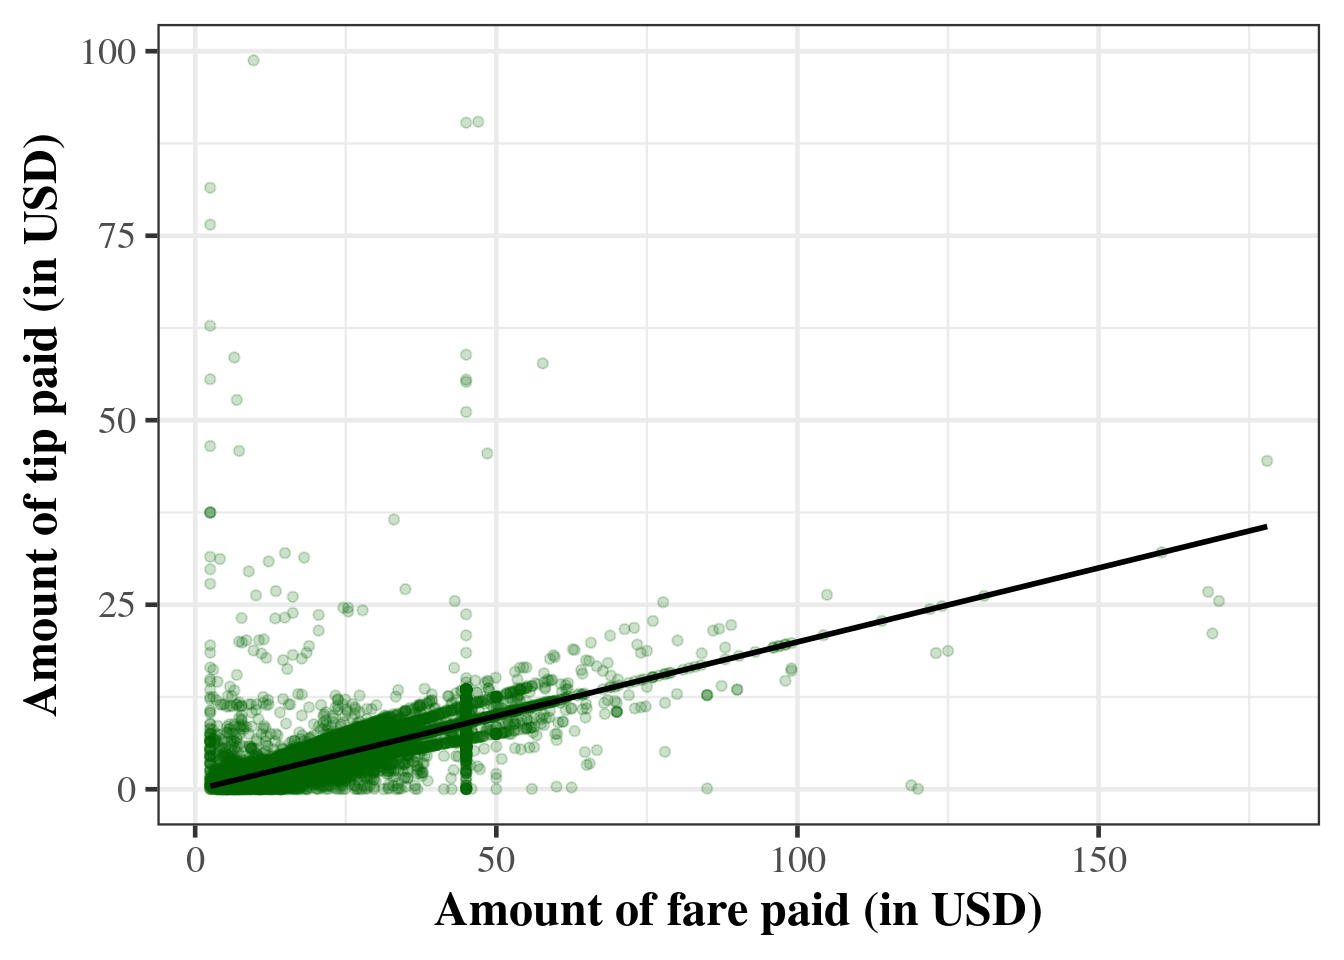
\includegraphics{bigdata_files/figure-latex/unnamed-chunk-148-1.pdf}

Now we can start adding the pick-up and drop-off locations of cap trips.

\begin{Shaded}
\begin{Highlighting}[]
\CommentTok{\# add pick{-}up locations to plot}
\NormalTok{locations }\SpecialCharTok{+} 
     \FunctionTok{geom\_point}\NormalTok{(}\FunctionTok{aes}\NormalTok{(}\AttributeTok{x=}\NormalTok{start\_long, }\AttributeTok{y=}\NormalTok{start\_lat),}
                \AttributeTok{color=}\StringTok{"orange"}\NormalTok{,}
                \AttributeTok{size =} \FloatTok{0.1}\NormalTok{,}
                \AttributeTok{alpha =} \FloatTok{0.2}\NormalTok{)}
\end{Highlighting}
\end{Shaded}

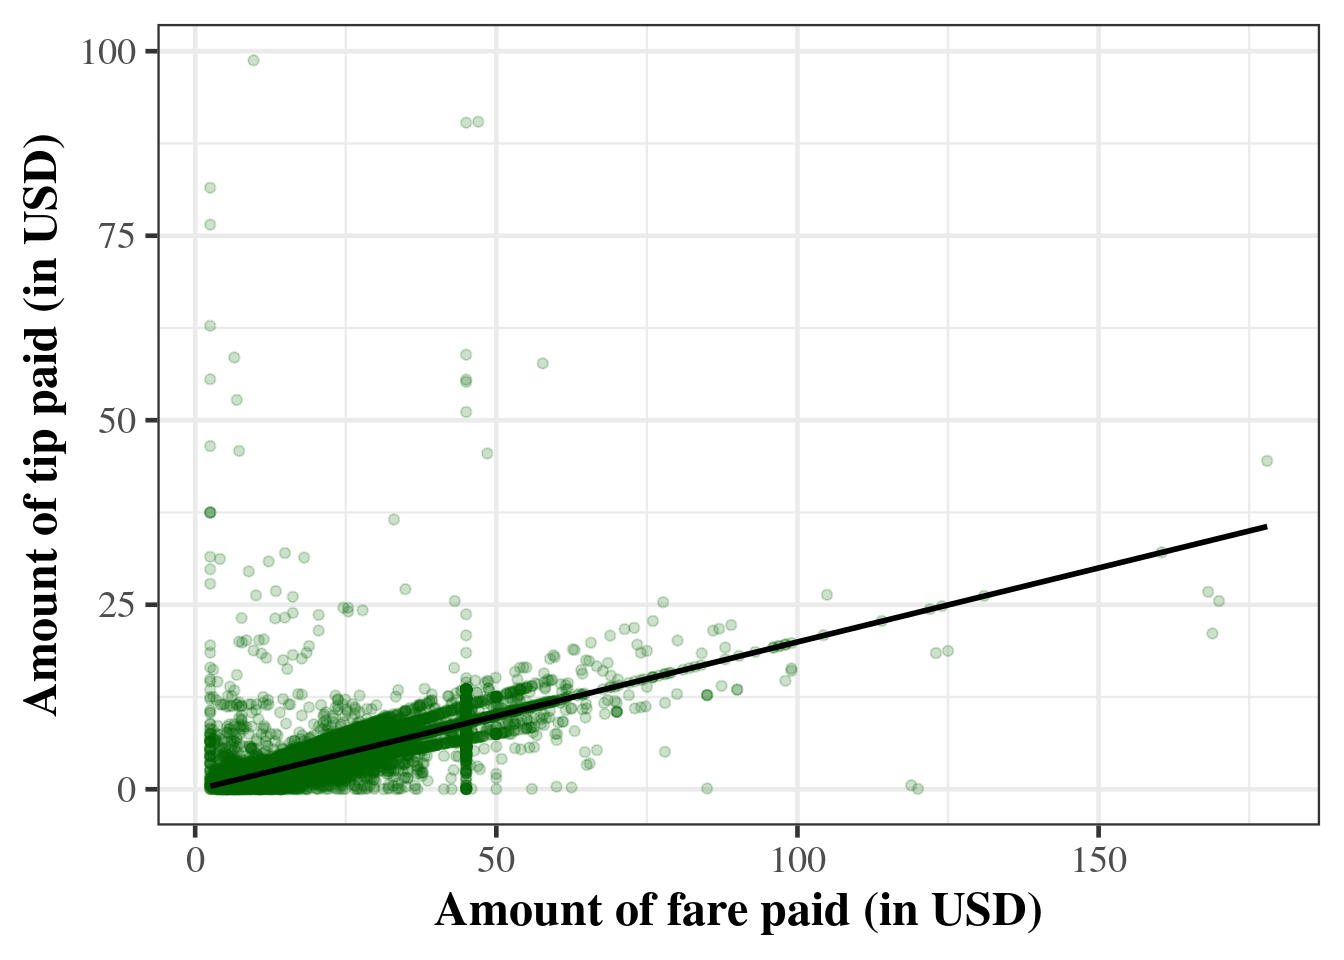
\includegraphics{bigdata_files/figure-latex/unnamed-chunk-149-1.pdf}

As to be expected, most of the trips start in Manhattan. Now let's look at where trips end.

\begin{Shaded}
\begin{Highlighting}[]
\CommentTok{\# add pick{-}up locations to plot}
\NormalTok{locations }\SpecialCharTok{+}
     \FunctionTok{geom\_point}\NormalTok{(}\FunctionTok{aes}\NormalTok{(}\AttributeTok{x=}\NormalTok{dest\_long, }\AttributeTok{y=}\NormalTok{dest\_lat),}
                \AttributeTok{color=}\StringTok{"steelblue"}\NormalTok{,}
                \AttributeTok{size =} \FloatTok{0.1}\NormalTok{,}
                \AttributeTok{alpha =} \FloatTok{0.2}\NormalTok{) }\SpecialCharTok{+}
     \FunctionTok{geom\_point}\NormalTok{(}\FunctionTok{aes}\NormalTok{(}\AttributeTok{x=}\NormalTok{start\_long, }\AttributeTok{y=}\NormalTok{start\_lat),}
                \AttributeTok{color=}\StringTok{"orange"}\NormalTok{,}
                \AttributeTok{size =} \FloatTok{0.1}\NormalTok{,}
                \AttributeTok{alpha =} \FloatTok{0.2}\NormalTok{)}
\end{Highlighting}
\end{Shaded}

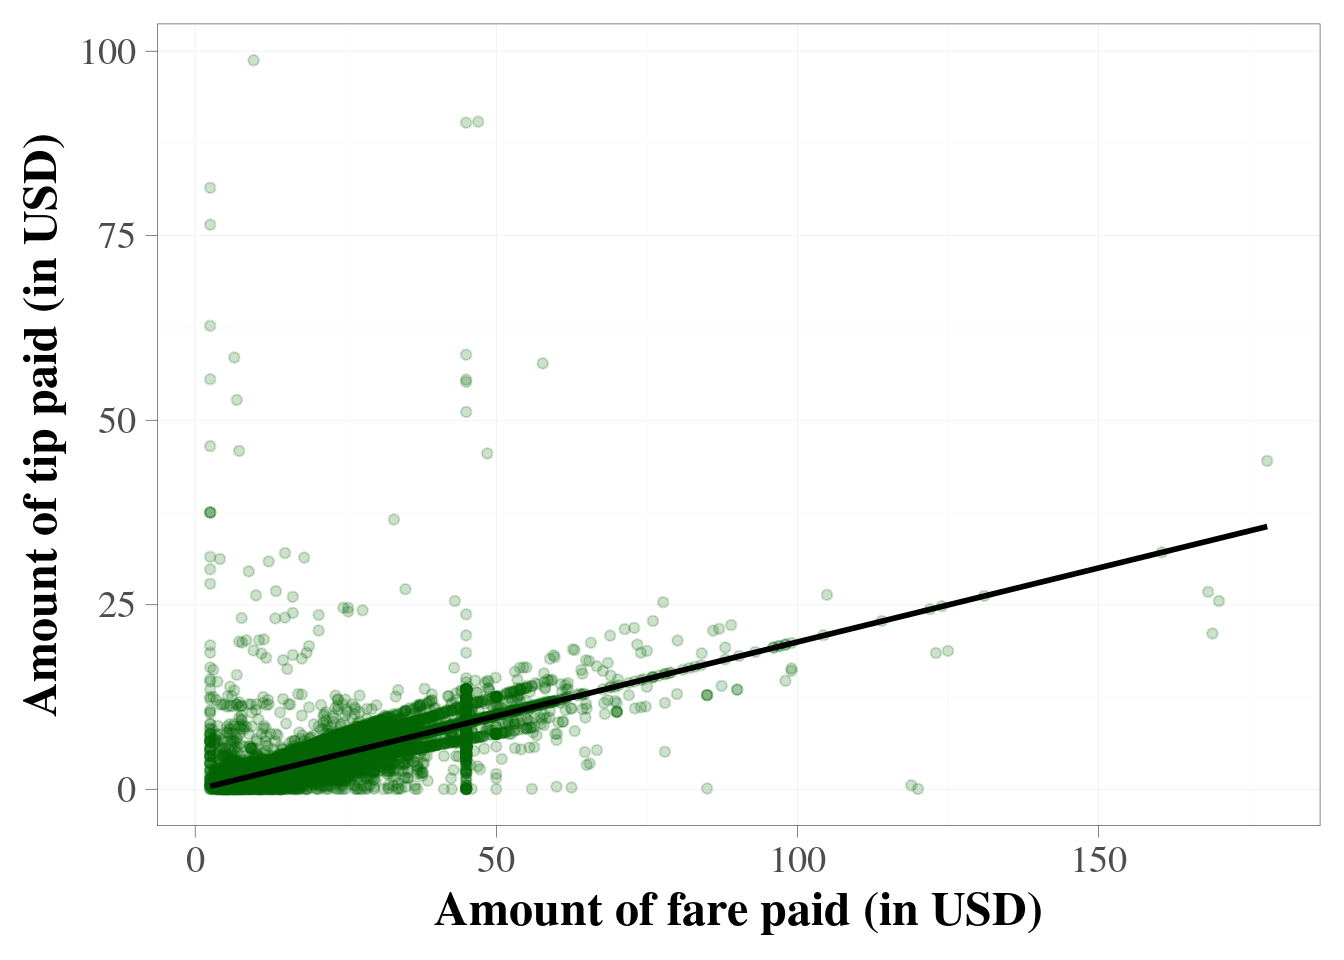
\includegraphics{bigdata_files/figure-latex/unnamed-chunk-150-1.pdf}

Incidentally, more trips tend to end outside of Manhattan. And the destinations seem to be broader spread across the city then the pick-up locations. Most destinations are still in Manhattan, though.

Now let's have a look at how this picture changes depending on the time of the day.

\begin{Shaded}
\begin{Highlighting}[]
\CommentTok{\# pick{-}up locations }
\NormalTok{locations }\SpecialCharTok{+}
     \FunctionTok{geom\_point}\NormalTok{(}\FunctionTok{aes}\NormalTok{(}\AttributeTok{x=}\NormalTok{start\_long, }\AttributeTok{y=}\NormalTok{start\_lat),}
                \AttributeTok{color=}\StringTok{"orange"}\NormalTok{,}
                \AttributeTok{size =} \FloatTok{0.1}\NormalTok{,}
                \AttributeTok{alpha =} \FloatTok{0.2}\NormalTok{) }\SpecialCharTok{+}
     \FunctionTok{facet\_wrap}\NormalTok{(}\FunctionTok{vars}\NormalTok{(time\_of\_day))}
\end{Highlighting}
\end{Shaded}

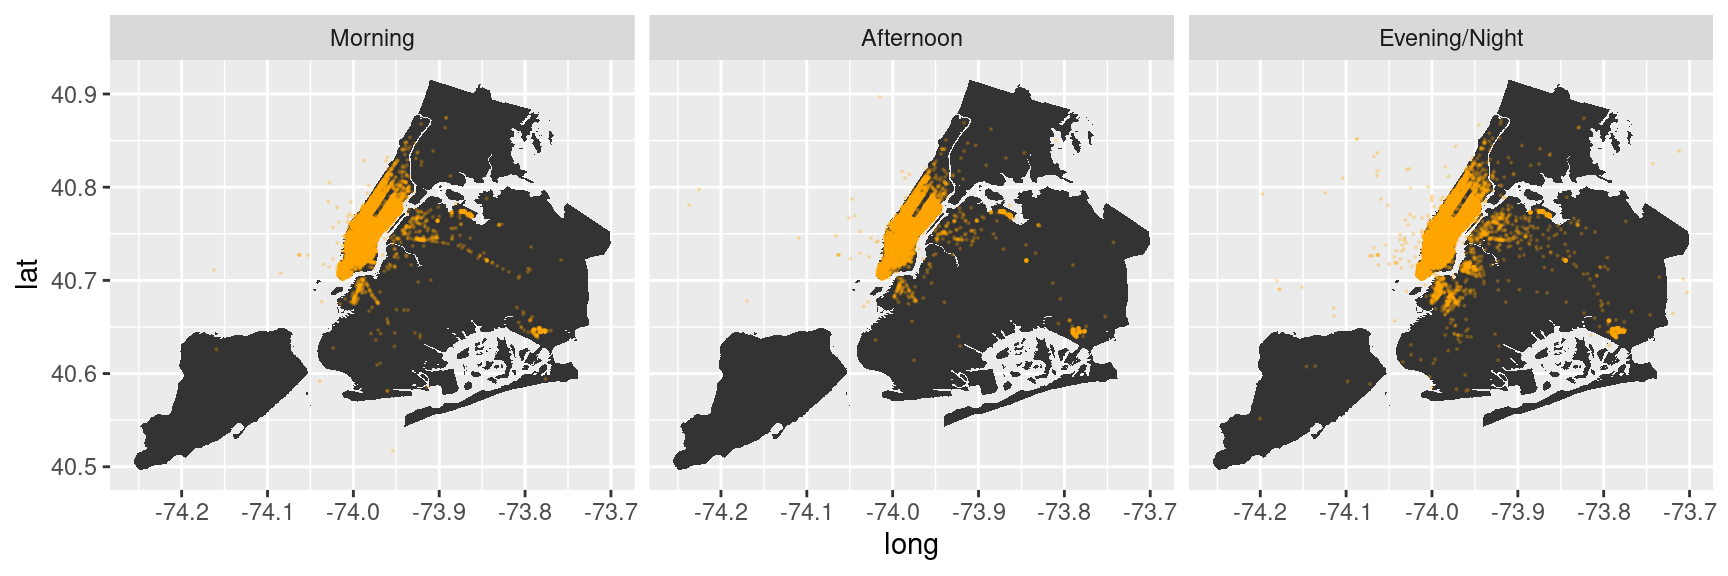
\includegraphics{bigdata_files/figure-latex/unnamed-chunk-151-1.pdf}

\begin{Shaded}
\begin{Highlighting}[]
\CommentTok{\# drop{-}off locations }
\NormalTok{locations }\SpecialCharTok{+}
     \FunctionTok{geom\_point}\NormalTok{(}\FunctionTok{aes}\NormalTok{(}\AttributeTok{x=}\NormalTok{dest\_long, }\AttributeTok{y=}\NormalTok{dest\_lat),}
                \AttributeTok{color=}\StringTok{"steelblue"}\NormalTok{,}
                \AttributeTok{size =} \FloatTok{0.1}\NormalTok{,}
                \AttributeTok{alpha =} \FloatTok{0.2}\NormalTok{) }\SpecialCharTok{+}
     \FunctionTok{facet\_wrap}\NormalTok{(}\FunctionTok{vars}\NormalTok{(time\_of\_day))}
\end{Highlighting}
\end{Shaded}

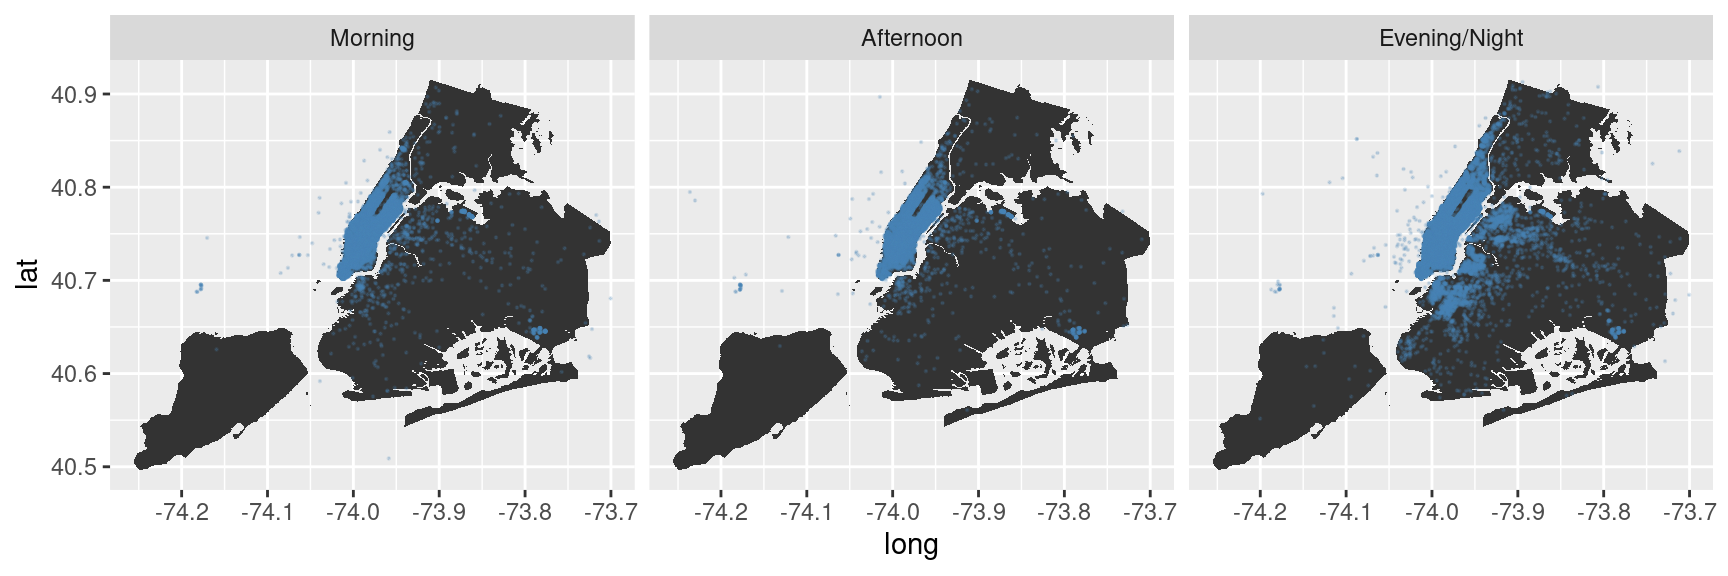
\includegraphics{bigdata_files/figure-latex/unnamed-chunk-152-1.pdf}

Alternatively, we can plot the hours on a continuous scale.

\begin{Shaded}
\begin{Highlighting}[]
\CommentTok{\# drop{-}off locations }
\NormalTok{locations }\SpecialCharTok{+}
     \FunctionTok{geom\_point}\NormalTok{(}\FunctionTok{aes}\NormalTok{(}\AttributeTok{x=}\NormalTok{dest\_long, }\AttributeTok{y=}\NormalTok{dest\_lat, }\AttributeTok{color =}\NormalTok{ start\_time ),}
                \AttributeTok{size =} \FloatTok{0.1}\NormalTok{,}
                \AttributeTok{alpha =} \FloatTok{0.2}\NormalTok{) }\SpecialCharTok{+}
     \FunctionTok{scale\_colour\_gradient2}\NormalTok{( }\AttributeTok{low =} \StringTok{"red"}\NormalTok{, }\AttributeTok{mid =} \StringTok{"yellow"}\NormalTok{, }\AttributeTok{high =} \StringTok{"red"}\NormalTok{,}
                             \AttributeTok{midpoint =} \DecValTok{12}\NormalTok{)}
\end{Highlighting}
\end{Shaded}

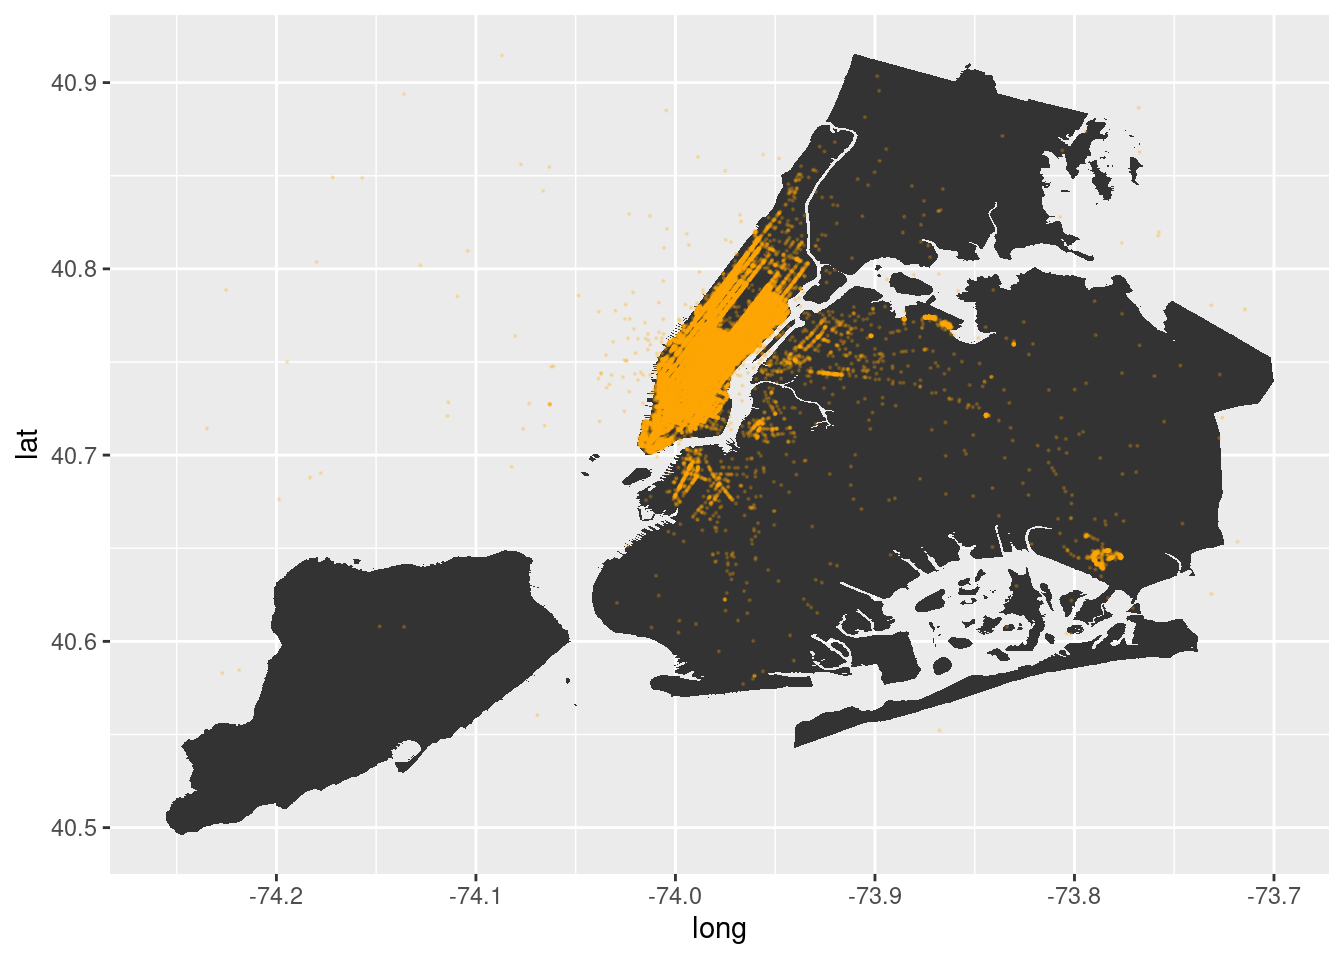
\includegraphics{bigdata_files/figure-latex/unnamed-chunk-153-1.pdf}

\hypertarget{excursus-change-color-schemes}{%
\section{Excursus: change color schemes}\label{excursus-change-color-schemes}}

In the example above we use \texttt{scale\_colour\_gradient2()} to modify the color gradient used to visualize the start time of taxi trips. By default, ggplot would plot the following (default gradient color setting):

\begin{Shaded}
\begin{Highlighting}[]
\CommentTok{\# drop{-}off locations }
\NormalTok{locations }\SpecialCharTok{+}
     \FunctionTok{geom\_point}\NormalTok{(}\FunctionTok{aes}\NormalTok{(}\AttributeTok{x=}\NormalTok{dest\_long, }\AttributeTok{y=}\NormalTok{dest\_lat, }\AttributeTok{color =}\NormalTok{ start\_time ),}
                \AttributeTok{size =} \FloatTok{0.1}\NormalTok{,}
                \AttributeTok{alpha =} \FloatTok{0.2}\NormalTok{) }
\end{Highlighting}
\end{Shaded}

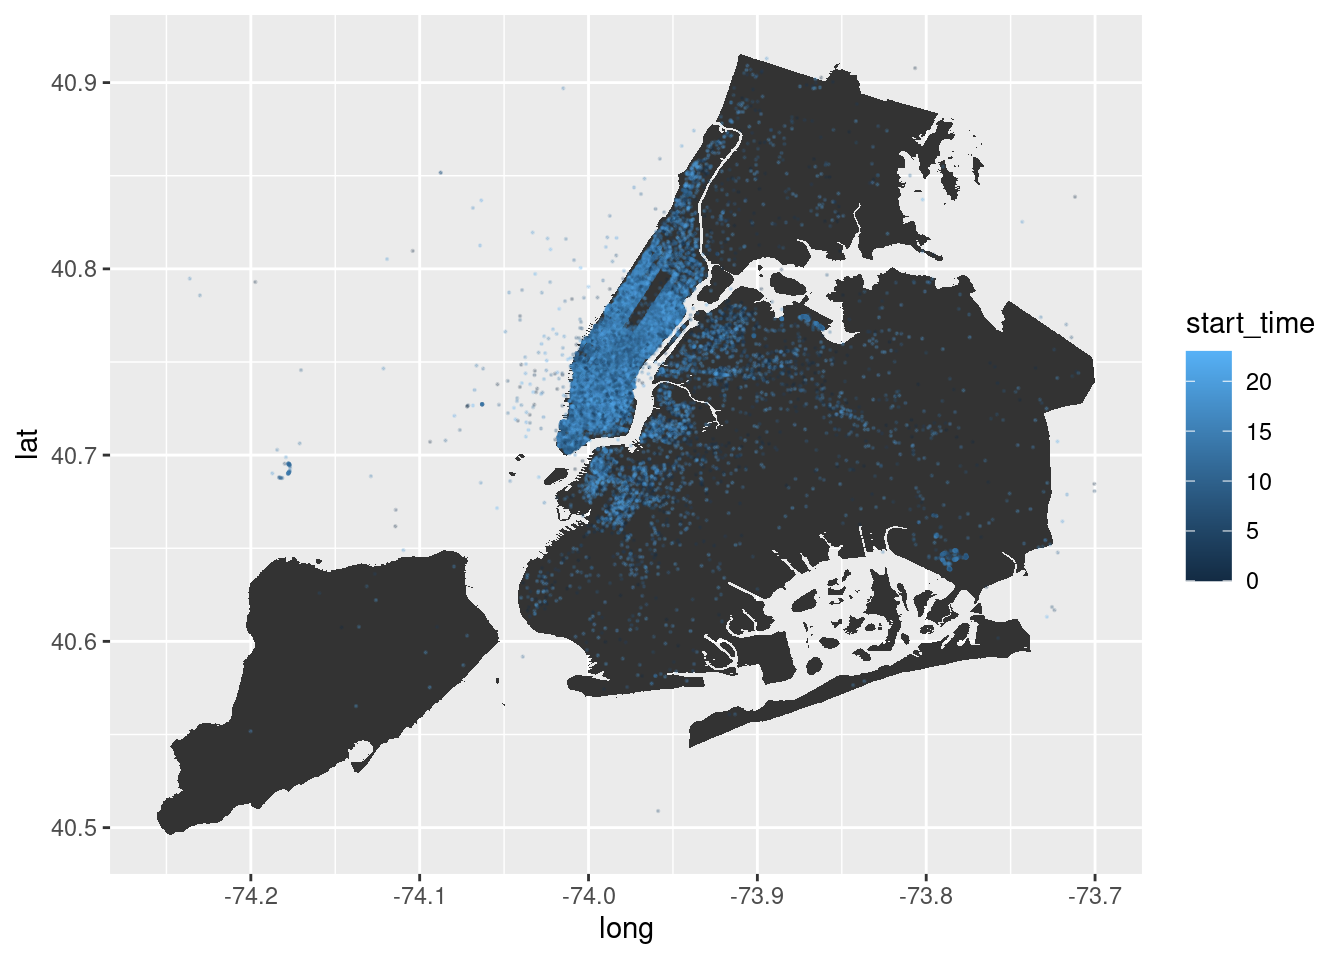
\includegraphics{bigdata_files/figure-latex/unnamed-chunk-154-1.pdf}

\texttt{ggplot2} offers various functions to modify the color scales used in a plot. In the case of the example above, we visualize values of a continuous variable. Hence we use a gradient color scale. In case of categorical variables we need to modify the default discrete color scale.

Recall the plot illustrating tipping behavior, where we highlight in which observations the client payd with credit card, cash, etc.

\begin{Shaded}
\begin{Highlighting}[]
\CommentTok{\# indicate natural numbers}
\NormalTok{taxi[, dollar\_paid }\SpecialCharTok{:}\ErrorTok{=} \FunctionTok{ifelse}\NormalTok{(tip\_amount }\SpecialCharTok{==} \FunctionTok{round}\NormalTok{(tip\_amount,}\DecValTok{0}\NormalTok{), }\StringTok{"Full"}\NormalTok{, }\StringTok{"Fraction"}\NormalTok{),]}


\CommentTok{\# extended x/y plot}
\NormalTok{taxiplot }\SpecialCharTok{+}
     \FunctionTok{geom\_point}\NormalTok{(}\AttributeTok{alpha=}\FloatTok{0.2}\NormalTok{, }\FunctionTok{aes}\NormalTok{(}\AttributeTok{color=}\NormalTok{payment\_type)) }\SpecialCharTok{+}
     \FunctionTok{facet\_wrap}\NormalTok{(}\StringTok{"dollar\_paid"}\NormalTok{)}
\end{Highlighting}
\end{Shaded}

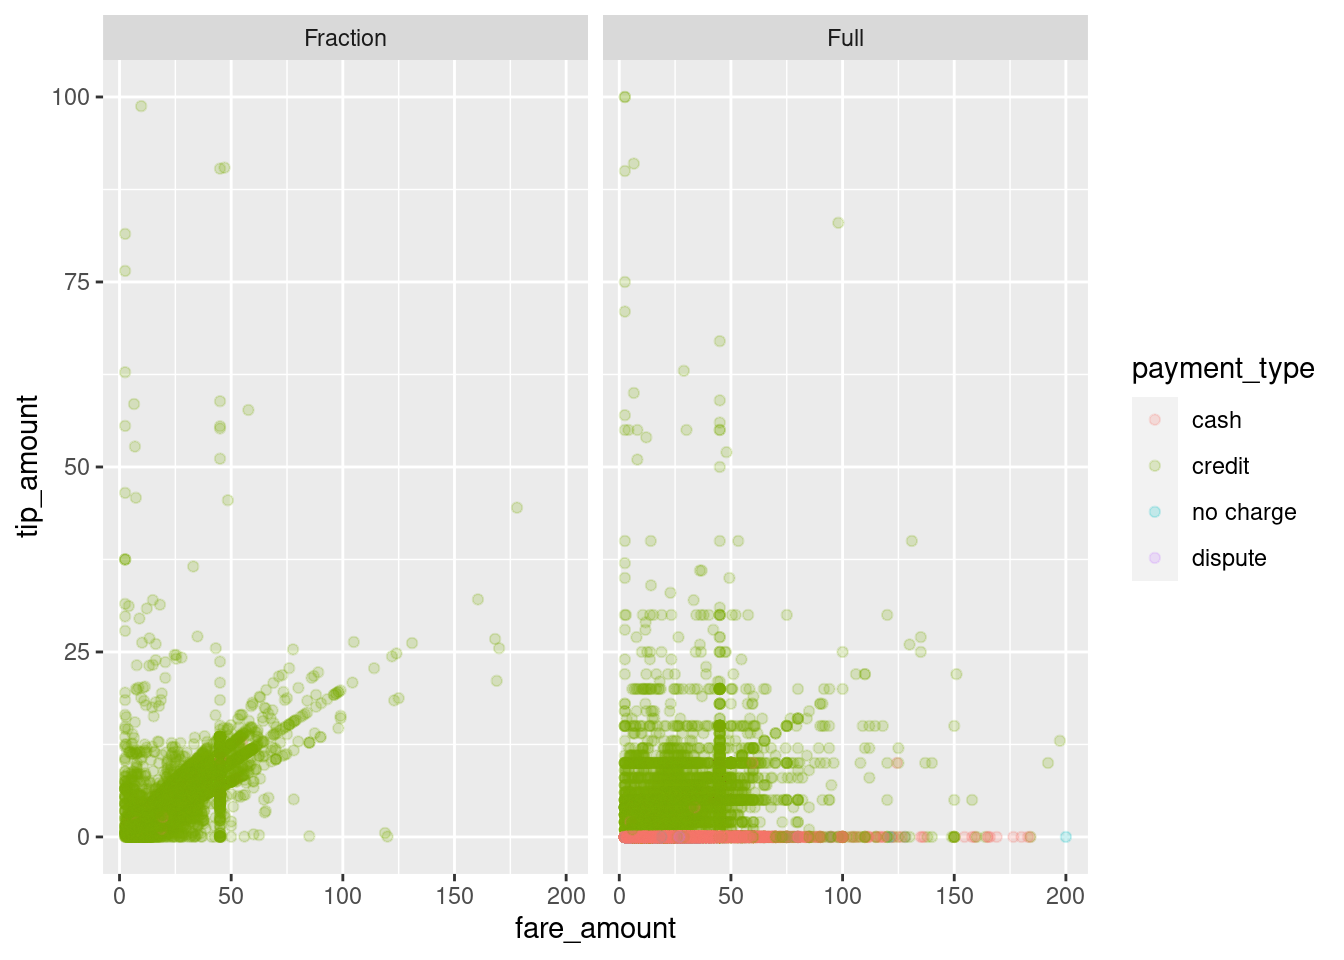
\includegraphics{bigdata_files/figure-latex/unnamed-chunk-155-1.pdf}

Since we do not further specify the discrete color scheme to be used, ggplot simply uses its default color scheme for this plot. We can change this as follows.

\begin{Shaded}
\begin{Highlighting}[]
\CommentTok{\# indicate natural numbers}
\NormalTok{taxi[, dollar\_paid }\SpecialCharTok{:}\ErrorTok{=} \FunctionTok{ifelse}\NormalTok{(tip\_amount }\SpecialCharTok{==} \FunctionTok{round}\NormalTok{(tip\_amount,}\DecValTok{0}\NormalTok{), }\StringTok{"Full"}\NormalTok{, }\StringTok{"Fraction"}\NormalTok{),]}


\CommentTok{\# extended x/y plot}
\NormalTok{taxiplot }\SpecialCharTok{+}
     \FunctionTok{geom\_point}\NormalTok{(}\AttributeTok{alpha=}\FloatTok{0.2}\NormalTok{, }\FunctionTok{aes}\NormalTok{(}\AttributeTok{color=}\NormalTok{payment\_type)) }\SpecialCharTok{+}
     \FunctionTok{facet\_wrap}\NormalTok{(}\StringTok{"dollar\_paid"}\NormalTok{) }\SpecialCharTok{+}
     \FunctionTok{scale\_color\_discrete}\NormalTok{(}\AttributeTok{type =} \FunctionTok{c}\NormalTok{(}\StringTok{"red"}\NormalTok{, }\StringTok{"steelblue"}\NormalTok{, }\StringTok{"orange"}\NormalTok{, }\StringTok{"purple"}\NormalTok{))}
\end{Highlighting}
\end{Shaded}

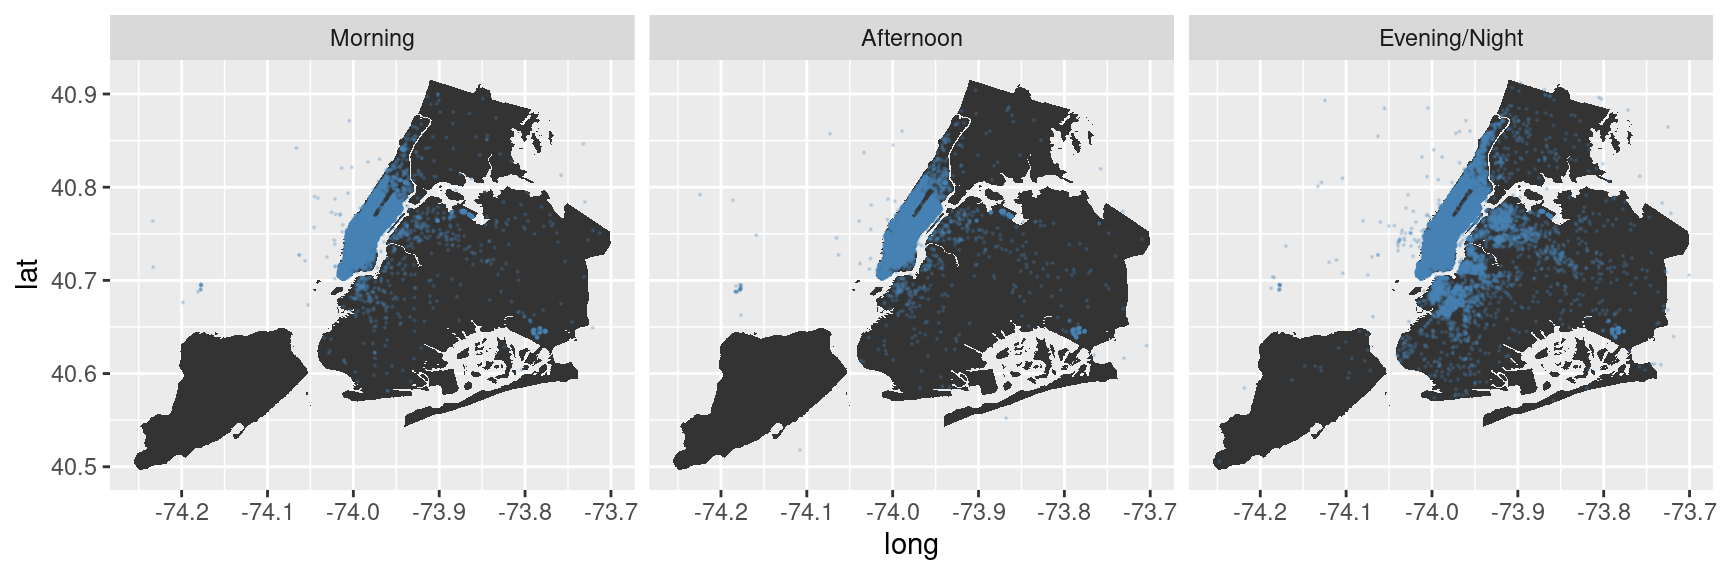
\includegraphics{bigdata_files/figure-latex/unnamed-chunk-156-1.pdf}

\hypertarget{cloud-services-for-big-data-analytics}{%
\chapter{Cloud Services for Big Data Analytics}\label{cloud-services-for-big-data-analytics}}

So far we have focused on how to deal with large amounts of data and/or computationally demanding tasks on our local machines (desktop/laptop). A key aspect of this course has thus been in a first step to understand why our local machine is struggling with a data analysis task when there is a large amount of data to be processed. In a second step we have looked into practical solutions to these challenges. These solutions are in essence tools (in this course particularly tools provided in the R environment) to use the key components of our computing environment (CPU, RAM, mass storage) most efficiently:

\begin{itemize}
\tightlist
\item
  Computationally intense tasks (but not pushing RAM to the limit): parallelization, using several CPU cores (nodes) in parallel.
\item
  Memory-intense tasks (data still fits into RAM): efficient memory allocation (\texttt{data.table}-package).
\item
  Memory-intense tasks (data does not fit into RAM): efficient use of virtual memory (use parts of mass storage device as virtual memory).
\item
  Big Data storage: efficient storage (avoid redundancies) and efficient access (speed) with RDBMSs (here: SQLite).
\end{itemize}

In practice, data sets might be too large for our local machine even if we take all of the techniques listed above into account. That is, a parallelized task might still take ages to complete because our local machine has too few cores available, a task involving virtual memory would use up way too much space on our hard-disk, running a large SQL database locally would use up too much resources, etc.

In such situations, we have to think about horizontal and vertical scaling beyond our local machine. That is, we outsource tasks to a bigger machine (or a cluster of machines) to which our local computer is connected over the Internet (or over a local network). While a decade or two ago most organizations had their own large centrally hosted machines (database servers, cluster computers) for such tasks, today they often rely on third-party solutions \emph{`in the cloud'}. That is, specialized companies provide flexible access to computing resources that can be easily accessed via a broadband Internet-connection and rented on an hourly (or even minutes and seconds) basis. Given the obvious economies of scale in this line of business, a few large players have emerged who practically dominate most of the global market:

\begin{itemize}
\tightlist
\item
  \href{https://aws.amazon.com/}{Amazon Web Services (AWS)}.
\item
  \href{https://azure.microsoft.com/en-us/}{Microsoft Azure}
\item
  \href{https://cloud.google.com/}{Google Cloud Platform}
\item
  \href{https://www.ibm.com/cloud/}{IBM Cloud}
\item
  \href{https://www.alibabacloud.com/}{Alibaba Cloud}
\item
  \href{https://intl.cloud.tencent.com/}{Tencent Cloud}
\item
  \ldots{}
\end{itemize}

For details on what some of the largest platforms provide, see the overview in the online chapter to \citet{walkowiak_2016} \href{https://www.packtpub.com/sites/default/files/downloads/5396_6457OS_PushingRFurther.pdf}{`Pushing R Further'}.

When we use such cloud services to \emph{scale up} (vertical scaling) the computing resources, the transition from our local implementation of a data analytics task to the cloud implementation is often rather simple. Once we have set up a cloud instance and figured out how to communicate with it, we typically can even run the exact same R-script locally or in the cloud. This is usually the case for parallelized tasks (simply run the same script on a machine with more cores), in-memory tasks (rent a machine with more RAM but still use \texttt{data.table()} etc.), and working with an SQL database (simply set up the database in the cloud instead of locally).

However, for really memory-intense tasks, the cloud provides options to \emph{scale out} (horizontal scaling). Meaning, a task is distributed among a cluster of computing instances/servers. The implementation of such data analytics tasks is based on a paradigm that we rather do not encounter when working locally: \emph{Map/Reduce} (implemented in the \emph{Hadoop} framework).

In the following we look first at scaling up more familiar approaches with the help of the cloud and then look at the Map/Reduce concept and how it can be applied in \emph{Hadoop} running on cloud instances.

\hypertarget{scaling-up-in-the-cloud}{%
\section{Scaling up in the Cloud}\label{scaling-up-in-the-cloud}}

In the following examples we use different cloud services provided by AWS. See the online chapter to \citet{walkowiak_2016} \href{https://www.packtpub.com/sites/default/files/downloads/5396_6457OS_PushingRFurther.pdf}{`Pushing R Further'} for how to set up an AWS account and the basics for how to set up AWS instances. The examples below are based on the assumption that the EC2 instance and RStudio Server have been set up essentially as explained in \href{https://www.packtpub.com/sites/default/files/downloads/5396_6457OS_PushingRFurther.pdf}{`Pushing R Further'}, pages 22-38. However, AWS changed a few things regarding the way their linux machines are set up since the online chapter was published first. In order to install core R on your ec2 instance, use the following command in the terminal (instead of \texttt{sudo\ yum\ install\ R}):

\begin{Shaded}
\begin{Highlighting}[]
\FunctionTok{sudo}\NormalTok{ amazon{-}linux{-}extras install R3.4}
\end{Highlighting}
\end{Shaded}

and confirm the installation of additional dependencies with \texttt{y}. In a second step, we install the latest CentOS 6-7 version of RStudio Server with the following commands.

\begin{Shaded}
\begin{Highlighting}[]
\CommentTok{\# April 2020}
\FunctionTok{wget}\NormalTok{ https://download2.rstudio.org/server/centos6/x86\_64/rstudio{-}server{-}rhel{-}1.2.5033{-}x86\_64.rpm}
\FunctionTok{sudo}\NormalTok{ yum install rstudio{-}server{-}rhel{-}1.2.5033{-}x86\_64.rpm}
\end{Highlighting}
\end{Shaded}

\hypertarget{parallelization-with-an-ec2-instance}{%
\subsection{Parallelization with an EC2 instance}\label{parallelization-with-an-ec2-instance}}

This short tutorial illustrates how to scale the computation of clustered standard errors shown in Lecture 3 up by running it on an AWS EC2 instance. Below we use the same source code as in the original example (see \href{https://github.com/umatter/BigData/blob/master/materials/notes/03_computation_memory.Rmd}{\texttt{03\_computation\_memory.Rmd}}). Note that there are a few things that we need to keep in mind in order to make the script run on an AWS EC2 instance in RStudio Server.

First, our EC2 instance is a Linux machine. Most of you are probably rather used to running R on a Mac or Windows PC. When running R on a Linux machine, there is an additional step to install R packages (at least for most of the packages): R packages need to be compiled before they can be installed. The command to install packages is exactly the same (\texttt{install.packages()}) and normally you only notice a slight difference in the output shown in the R console during installation (and the installation process takes a little longer than what you are used to). Apart from that, using R via RStudio Server in the cloud looks/feels very similar if not identical as when using R/RStudio locally.

Now, let's go through the bootstrap example. First, let's run the non-parallel implementation of the script. When executing the code below line-by-line, you will notice that essentially all parts of the script work exactly as on your local machine. This is one of the great advantages of running R/RStudio Server in the cloud. You can implement your entire data analysis locally (based on a small sample), test it locally, and then move it to the cloud and run it on a larger scale in exactly the same way (even with the same GUI).

\begin{Shaded}
\begin{Highlighting}[]
\CommentTok{\# CASE STUDY: PARALLEL {-}{-}{-}{-}{-}{-}{-}{-}{-}{-}{-}{-}{-}{-}{-}{-}{-}{-}{-}{-}{-}{-}{-}{-}{-}{-}{-}}

\CommentTok{\# install packages}
\FunctionTok{install.packages}\NormalTok{(}\StringTok{"data.table"}\NormalTok{)}
\FunctionTok{install.packages}\NormalTok{(}\StringTok{"doSNOW"}\NormalTok{)}

\CommentTok{\# load packages}
\FunctionTok{library}\NormalTok{(data.table)}


\DocumentationTok{\#\# {-}{-}{-}{-}{-}{-}{-}{-}{-}{-}{-}{-}{-}{-}{-}{-}{-}{-}{-}{-}{-}{-}{-}{-}{-}{-}{-}{-}{-}{-}{-}{-}{-}{-}{-}{-}{-}{-}{-}{-}{-}{-}{-}{-}{-}{-}{-}{-}{-}{-}{-}{-}{-}{-}{-}{-}{-}{-}{-}{-}{-}{-}{-}{-}{-}{-}{-}{-}{-}{-}{-}{-}}
\NormalTok{stopdata }\OtherTok{\textless{}{-}} \FunctionTok{read.csv}\NormalTok{(}\StringTok{"https://vincentarelbundock.github.io/Rdatasets/csv/carData/MplsStops.csv"}\NormalTok{)}

\DocumentationTok{\#\# {-}{-}{-}{-}{-}{-}{-}{-}{-}{-}{-}{-}{-}{-}{-}{-}{-}{-}{-}{-}{-}{-}{-}{-}{-}{-}{-}{-}{-}{-}{-}{-}{-}{-}{-}{-}{-}{-}{-}{-}{-}{-}{-}{-}{-}{-}{-}{-}{-}{-}{-}{-}{-}{-}{-}{-}{-}{-}{-}{-}{-}{-}{-}{-}{-}{-}{-}{-}{-}{-}{-}{-}}
\CommentTok{\# remove incomplete obs}
\NormalTok{stopdata }\OtherTok{\textless{}{-}} \FunctionTok{na.omit}\NormalTok{(stopdata)}
\CommentTok{\# code dependent var}
\NormalTok{stopdata}\SpecialCharTok{$}\NormalTok{vsearch }\OtherTok{\textless{}{-}} \DecValTok{0}
\NormalTok{stopdata}\SpecialCharTok{$}\NormalTok{vsearch[stopdata}\SpecialCharTok{$}\NormalTok{vehicleSearch}\SpecialCharTok{==}\StringTok{"YES"}\NormalTok{] }\OtherTok{\textless{}{-}} \DecValTok{1}
\CommentTok{\# code explanatory var}
\NormalTok{stopdata}\SpecialCharTok{$}\NormalTok{white }\OtherTok{\textless{}{-}} \DecValTok{0}
\NormalTok{stopdata}\SpecialCharTok{$}\NormalTok{white[stopdata}\SpecialCharTok{$}\NormalTok{race}\SpecialCharTok{==}\StringTok{"White"}\NormalTok{] }\OtherTok{\textless{}{-}} \DecValTok{1}

\DocumentationTok{\#\# {-}{-}{-}{-}{-}{-}{-}{-}{-}{-}{-}{-}{-}{-}{-}{-}{-}{-}{-}{-}{-}{-}{-}{-}{-}{-}{-}{-}{-}{-}{-}{-}{-}{-}{-}{-}{-}{-}{-}{-}{-}{-}{-}{-}{-}{-}{-}{-}{-}{-}{-}{-}{-}{-}{-}{-}{-}{-}{-}{-}{-}{-}{-}{-}{-}{-}{-}{-}{-}{-}{-}{-}}
\NormalTok{model }\OtherTok{\textless{}{-}}\NormalTok{ vsearch }\SpecialCharTok{\textasciitilde{}}\NormalTok{ white }\SpecialCharTok{+} \FunctionTok{factor}\NormalTok{(policePrecinct)}

\DocumentationTok{\#\# {-}{-}{-}{-}{-}{-}{-}{-}{-}{-}{-}{-}{-}{-}{-}{-}{-}{-}{-}{-}{-}{-}{-}{-}{-}{-}{-}{-}{-}{-}{-}{-}{-}{-}{-}{-}{-}{-}{-}{-}{-}{-}{-}{-}{-}{-}{-}{-}{-}{-}{-}{-}{-}{-}{-}{-}{-}{-}{-}{-}{-}{-}{-}{-}{-}{-}{-}{-}{-}{-}{-}{-}}
\NormalTok{fit }\OtherTok{\textless{}{-}} \FunctionTok{lm}\NormalTok{(model, stopdata)}
\FunctionTok{summary}\NormalTok{(fit)}


\CommentTok{\# bootstrapping: normal approach}

\DocumentationTok{\#\# {-}{-}{-}{-}message=FALSE{-}{-}{-}{-}{-}{-}{-}{-}{-}{-}{-}{-}{-}{-}{-}{-}{-}{-}{-}{-}{-}{-}{-}{-}{-}{-}{-}{-}{-}{-}{-}{-}{-}{-}{-}{-}{-}{-}{-}{-}{-}{-}{-}{-}{-}{-}{-}{-}{-}{-}{-}{-}{-}{-}{-}}

\CommentTok{\# set the \textquotesingle{}seed\textquotesingle{} for random numbers (makes the example reproducible)}
\FunctionTok{set.seed}\NormalTok{(}\DecValTok{2}\NormalTok{)}

\CommentTok{\# set number of bootstrap iterations}
\NormalTok{B }\OtherTok{\textless{}{-}} \DecValTok{50}
\CommentTok{\# get selection of precincts}
\NormalTok{precincts }\OtherTok{\textless{}{-}} \FunctionTok{unique}\NormalTok{(stopdata}\SpecialCharTok{$}\NormalTok{policePrecinct)}
\CommentTok{\# container for coefficients}
\NormalTok{boot\_coefs }\OtherTok{\textless{}{-}} \FunctionTok{matrix}\NormalTok{(}\ConstantTok{NA}\NormalTok{, }\AttributeTok{nrow =}\NormalTok{ B, }\AttributeTok{ncol =} \DecValTok{2}\NormalTok{)}
\CommentTok{\# draw bootstrap samples, estimate model for each sample}
\ControlFlowTok{for}\NormalTok{ (i }\ControlFlowTok{in} \DecValTok{1}\SpecialCharTok{:}\NormalTok{B) \{}
  
  \CommentTok{\# draw sample of precincts (cluster level)}
\NormalTok{  precincts\_i }\OtherTok{\textless{}{-}} \FunctionTok{sample}\NormalTok{(precincts, }\AttributeTok{size =} \DecValTok{5}\NormalTok{, }\AttributeTok{replace =} \ConstantTok{TRUE}\NormalTok{)}
  \CommentTok{\# get observations}
\NormalTok{  bs\_i }\OtherTok{\textless{}{-}} \FunctionTok{lapply}\NormalTok{(precincts\_i, }\ControlFlowTok{function}\NormalTok{(x) stopdata[stopdata}\SpecialCharTok{$}\NormalTok{policePrecinct}\SpecialCharTok{==}\NormalTok{x,])}
\NormalTok{  bs\_i }\OtherTok{\textless{}{-}} \FunctionTok{rbindlist}\NormalTok{(bs\_i)}
  
  \CommentTok{\# estimate model and record coefficients}
\NormalTok{  boot\_coefs[i,] }\OtherTok{\textless{}{-}} \FunctionTok{coef}\NormalTok{(}\FunctionTok{lm}\NormalTok{(model, bs\_i))[}\DecValTok{1}\SpecialCharTok{:}\DecValTok{2}\NormalTok{] }\CommentTok{\# ignore FE{-}coefficients}
\NormalTok{\}}

\DocumentationTok{\#\# {-}{-}{-}{-}{-}{-}{-}{-}{-}{-}{-}{-}{-}{-}{-}{-}{-}{-}{-}{-}{-}{-}{-}{-}{-}{-}{-}{-}{-}{-}{-}{-}{-}{-}{-}{-}{-}{-}{-}{-}{-}{-}{-}{-}{-}{-}{-}{-}{-}{-}{-}{-}{-}{-}{-}{-}{-}{-}{-}{-}{-}{-}{-}{-}{-}{-}{-}{-}{-}{-}{-}{-}}
\NormalTok{se\_boot }\OtherTok{\textless{}{-}} \FunctionTok{apply}\NormalTok{(boot\_coefs, }
                 \AttributeTok{MARGIN =} \DecValTok{2}\NormalTok{,}
                 \AttributeTok{FUN =}\NormalTok{ sd)}
\NormalTok{se\_boot}
\end{Highlighting}
\end{Shaded}

So far, we have only demonstrated that the simple implementation (non-parallel) works both locally and in the cloud. The real purpose of using an EC2 instance in this example is to make use of the fact that we can scale up our instance to have more CPU cores available for the parallel implementation of our bootstrap procedure. Recall that running the script below on our local machine will employ all cores available to an compute the bootstrap resampling in parallel on all these cores. Exactly the same thing happens when running the code below on our simple \texttt{t2.micro} instance. However this type of EC2 instance only has one core. You can check this when running the following line of code in RStudio Server (assuming the \texttt{doSNOW} package is installed and loaded):

\begin{Shaded}
\begin{Highlighting}[]
\NormalTok{parallel}\SpecialCharTok{::}\FunctionTok{detectCores}\NormalTok{()}
\end{Highlighting}
\end{Shaded}

When running the entire parallel implementation below, you will thus notice that it won't compute the bootstrap SE any faster than with the non-parallel version above. However, by simply initiating another EC2 type with more cores, we can distribute the workload across many CPU cores, using exactly the same R-script.

\begin{Shaded}
\begin{Highlighting}[]
\CommentTok{\# bootstrapping: parallel approaach}

\DocumentationTok{\#\# {-}{-}{-}{-}message=FALSE{-}{-}{-}{-}{-}{-}{-}{-}{-}{-}{-}{-}{-}{-}{-}{-}{-}{-}{-}{-}{-}{-}{-}{-}{-}{-}{-}{-}{-}{-}{-}{-}{-}{-}{-}{-}{-}{-}{-}{-}{-}{-}{-}{-}{-}{-}{-}{-}{-}{-}{-}{-}{-}{-}{-}}
\CommentTok{\# install.packages("doSNOW", "parallel")}
\CommentTok{\# load packages for parallel processing}
\FunctionTok{library}\NormalTok{(doSNOW)}

\CommentTok{\# get the number of cores available}
\NormalTok{ncores }\OtherTok{\textless{}{-}}\NormalTok{ parallel}\SpecialCharTok{::}\FunctionTok{detectCores}\NormalTok{()}
\CommentTok{\# set cores for parallel processing}
\NormalTok{ctemp }\OtherTok{\textless{}{-}} \FunctionTok{makeCluster}\NormalTok{(ncores) }\CommentTok{\# }
\FunctionTok{registerDoSNOW}\NormalTok{(ctemp)}


\CommentTok{\# set number of bootstrap iterations}
\NormalTok{B }\OtherTok{\textless{}{-}} \DecValTok{50}
\CommentTok{\# get selection of precincts}
\NormalTok{precincts }\OtherTok{\textless{}{-}} \FunctionTok{unique}\NormalTok{(stopdata}\SpecialCharTok{$}\NormalTok{policePrecinct)}
\CommentTok{\# container for coefficients}
\NormalTok{boot\_coefs }\OtherTok{\textless{}{-}} \FunctionTok{matrix}\NormalTok{(}\ConstantTok{NA}\NormalTok{, }\AttributeTok{nrow =}\NormalTok{ B, }\AttributeTok{ncol =} \DecValTok{2}\NormalTok{)}

\CommentTok{\# bootstrapping in parallel}
\NormalTok{boot\_coefs }\OtherTok{\textless{}{-}} 
  \FunctionTok{foreach}\NormalTok{(}\AttributeTok{i =} \DecValTok{1}\SpecialCharTok{:}\NormalTok{B, }\AttributeTok{.combine =}\NormalTok{ rbind, }\AttributeTok{.packages=}\StringTok{"data.table"}\NormalTok{) }\SpecialCharTok{\%dopar\%}\NormalTok{ \{}
    
    \CommentTok{\# draw sample of precincts (cluster level)}
\NormalTok{    precincts\_i }\OtherTok{\textless{}{-}} \FunctionTok{sample}\NormalTok{(precincts, }\AttributeTok{size =} \DecValTok{5}\NormalTok{, }\AttributeTok{replace =} \ConstantTok{TRUE}\NormalTok{)}
    \CommentTok{\# get observations}
\NormalTok{    bs\_i }\OtherTok{\textless{}{-}} \FunctionTok{lapply}\NormalTok{(precincts\_i, }\ControlFlowTok{function}\NormalTok{(x) stopdata[stopdata}\SpecialCharTok{$}\NormalTok{policePrecinct}\SpecialCharTok{==}\NormalTok{x,])}
\NormalTok{    bs\_i }\OtherTok{\textless{}{-}} \FunctionTok{rbindlist}\NormalTok{(bs\_i)}
    
    \CommentTok{\# estimate model and record coefficients}
    \FunctionTok{coef}\NormalTok{(}\FunctionTok{lm}\NormalTok{(model, bs\_i))[}\DecValTok{1}\SpecialCharTok{:}\DecValTok{2}\NormalTok{] }\CommentTok{\# ignore FE{-}coefficients}
    
\NormalTok{  \}}


\CommentTok{\# be a good citizen and stop the snow clusters}
\FunctionTok{stopCluster}\NormalTok{(}\AttributeTok{cl =}\NormalTok{ ctemp)}



\DocumentationTok{\#\# {-}{-}{-}{-}{-}{-}{-}{-}{-}{-}{-}{-}{-}{-}{-}{-}{-}{-}{-}{-}{-}{-}{-}{-}{-}{-}{-}{-}{-}{-}{-}{-}{-}{-}{-}{-}{-}{-}{-}{-}{-}{-}{-}{-}{-}{-}{-}{-}{-}{-}{-}{-}{-}{-}{-}{-}{-}{-}{-}{-}{-}{-}{-}{-}{-}{-}{-}{-}{-}{-}{-}{-}}
\NormalTok{se\_boot }\OtherTok{\textless{}{-}} \FunctionTok{apply}\NormalTok{(boot\_coefs, }
                 \AttributeTok{MARGIN =} \DecValTok{2}\NormalTok{,}
                 \AttributeTok{FUN =}\NormalTok{ sd)}
\NormalTok{se\_boot}
\end{Highlighting}
\end{Shaded}

\hypertarget{mass-storage-mariadb-on-an-ec2-instance}{%
\subsection{Mass Storage: MariaDB on an EC2 instance}\label{mass-storage-mariadb-on-an-ec2-instance}}

Once we have set up RStudio Server on an EC2 instance, we can run the SQLite examples demonstrated locally in Lecture 7 on it. There are no additional steps needed to install SQLite. However, when using RDBMSs in the cloud, we typically have a more sophisticated implementation than SQLite in mind. Particularly, we want to set up an actual RDBMS-server running in the cloud to which several clients can connect (via RStudio Server). The following example, based on \citet{walkowiak_2016}, guides you through the first step to set up such a database in the cloud. To keep things simple, the example sets up a database of the same data set as shown in the first SQLite example in Lecture 7, but this time with MariaDB on an EC2 instance in the cloud. For most of the installation steps you are referred to the respective pages in \citet{walkowiak_2016} (Chapter 5: 'MariaDB with R on a Amazon EC2 instance, pages 255ff). However, since some of the steps shown in the book are outdated, the example below hints to some alternative/additional steps needed to make the database run on an Ubuntu 18.04 machine.

After launching the EC2 instance on AWS, use the following terminal commands to install R:

\begin{Shaded}
\begin{Highlighting}[]
\CommentTok{\# update ubuntu packages}
 \FunctionTok{sudo}\NormalTok{ apt{-}get update}
 \FunctionTok{sudo}\NormalTok{ apt{-}get upgrade}
\end{Highlighting}
\end{Shaded}

\begin{Shaded}
\begin{Highlighting}[]
\FunctionTok{sudo}\NormalTok{ apt{-}get install r{-}base}
\end{Highlighting}
\end{Shaded}

and to install RStudio Server (on Ubuntu 18.04, as of April 2020):

\begin{Shaded}
\begin{Highlighting}[]
\FunctionTok{sudo}\NormalTok{ apt{-}get install gdebi{-}core}
\FunctionTok{wget}\NormalTok{ https://download2.rstudio.org/server/bionic/amd64/rstudio{-}server{-}1.2.5033{-}amd64.deb}
\FunctionTok{sudo}\NormalTok{ gdebi rstudio{-}server{-}1.2.5033{-}amd64.deb}
\end{Highlighting}
\end{Shaded}

Following \citet{walkowiak_2016} (pages 257f), we first set up a new user and give it permissions to \texttt{ssh} directly to the EC2 instance (this way we can then more easily upload data `for this user').

\begin{Shaded}
\begin{Highlighting}[]
\CommentTok{\# create user}
\FunctionTok{sudo}\NormalTok{ adduser umatter }
\end{Highlighting}
\end{Shaded}

When prompted for additional information just hit enter (for default). Now we can grant the user the permissions

\begin{Shaded}
\begin{Highlighting}[]
\FunctionTok{sudo}\NormalTok{ cp }\AttributeTok{{-}r}\NormalTok{ /home/ubuntu/.ssh /home/umatter/}
\BuiltInTok{cd}\NormalTok{ /home/umatter/}
\FunctionTok{sudo}\NormalTok{ chown }\AttributeTok{{-}R}\NormalTok{ umatter:umatter .ssh}
\end{Highlighting}
\end{Shaded}

Then install MariaDB as follows.

\begin{Shaded}
\begin{Highlighting}[]
\FunctionTok{sudo}\NormalTok{ apt update}
\FunctionTok{sudo}\NormalTok{ apt install mariadb{-}server}
\FunctionTok{sudo}\NormalTok{ apt install libmariadbclient{-}dev}
\FunctionTok{sudo}\NormalTok{ apt install libxml2{-}dev }\CommentTok{\# needed later (dependency for some R packages)}
\end{Highlighting}
\end{Shaded}

If prompted to set a password for the root database user (user with all database priviledges), type in and confirm the chosen password.\footnote{Below it is shown how to do this `manually', if not promted at this step.}

\hypertarget{data-import-3}{%
\subsubsection{Data import}\label{data-import-3}}

With the permissions set above, we can send data from the local machine directly to the instance via \texttt{ssh}. We use this to first transfer the raw data to the instance and then import it to the database.

The aim is to import the same simple data set \texttt{economics.csv} used in the local SQLite examples of Lecture 7. Following the instructions of \citet{walkowiak_2016}, pages 252 to 254, we upload the \texttt{economics.csv} file (instead of the example data used in \citet{walkowiak_2016}). Note that in all the code examples below, the username is \texttt{umatter}, and the IP-address will have to be replaced with the public IP-address of your EC2 instance.

Open a new terminal window and send the \texttt{economics.csv} data as follows to the instance.

\begin{Shaded}
\begin{Highlighting}[]
\CommentTok{\# from the directory where the key{-}file is stored...}
\FunctionTok{scp} \AttributeTok{{-}r} \AttributeTok{{-}i} \StringTok{"mariadb\_ec2.pem"}\NormalTok{ \textasciitilde{}/Desktop/economics.csv umatter@ec2{-}184{-}72{-}202{-}166.compute{-}1.amazonaws.com:\textasciitilde{}/}
\end{Highlighting}
\end{Shaded}

Then switch back to the terminal connected to the instance and start the MariaDB server.

\begin{Shaded}
\begin{Highlighting}[]
\CommentTok{\# start the MariaDB server}
\FunctionTok{sudo}\NormalTok{ service mysql start}
\CommentTok{\# log into the MariaDB client as root }
\FunctionTok{sudo}\NormalTok{ mysql }\AttributeTok{{-}uroot} 
\end{Highlighting}
\end{Shaded}

If not prompted to do so when installing MariaDB (see above), add a new root user in order to login to MariaDB without the \texttt{sudo} (here we simply set the password to `Password1').

\begin{Shaded}
\begin{Highlighting}[]
\KeywordTok{GRANT} \KeywordTok{ALL} \KeywordTok{PRIVILEGES} \KeywordTok{on} \OperatorTok{*}\NormalTok{.}\OperatorTok{*} \KeywordTok{to} \StringTok{\textquotesingle{}root\textquotesingle{}}\NormalTok{@}\StringTok{\textquotesingle{}localhost\textquotesingle{}} \KeywordTok{IDENTIFIED} \KeywordTok{BY} \StringTok{\textquotesingle{}Password1\textquotesingle{}}\NormalTok{;}
\KeywordTok{FLUSH} \KeywordTok{PRIVILEGES}\NormalTok{;}
\end{Highlighting}
\end{Shaded}

Restart the mysql server and log in with the database root user.

\begin{Shaded}
\begin{Highlighting}[]
\CommentTok{\# start the MariaDB server}
\FunctionTok{sudo}\NormalTok{ service mysql restart}
\CommentTok{\# log into the MariaDB client as root }
\ExtensionTok{mysql} \AttributeTok{{-}uroot} \AttributeTok{{-}p}
\end{Highlighting}
\end{Shaded}

Now we can initiate a new database called \texttt{data1}.

\begin{Shaded}
\begin{Highlighting}[]
\KeywordTok{CREATE} \KeywordTok{database}\NormalTok{ data1;}
\end{Highlighting}
\end{Shaded}

To work with the newly created database, we have to `select' it.

\begin{Shaded}
\begin{Highlighting}[]
\KeywordTok{USE}\NormalTok{ data1;}
\end{Highlighting}
\end{Shaded}

Then, we create the first table of our database and import data into it. Note that we only have to slightly adjust the former SQLite syntax to make this work (remove double quotes for field names). In addition, note that we can use the same field types as in the SQLite DB.\footnote{However, MariaDB is a much more sophisticated RDBMS than SQLite and comes with many more field types, see the official \href{https://mariadb.com/kb/en/library/data-types/}{list of supported data types}.}

\begin{Shaded}
\begin{Highlighting}[]
\CommentTok{{-}{-} Create the new table}
\KeywordTok{CREATE} \KeywordTok{TABLE}\NormalTok{ econ(}
\DataTypeTok{date} \DataTypeTok{DATE}\NormalTok{,}
\NormalTok{pce }\DataTypeTok{REAL}\NormalTok{,}
\NormalTok{pop }\DataTypeTok{INTEGER}\NormalTok{,}
\NormalTok{psavert }\DataTypeTok{REAL}\NormalTok{,}
\NormalTok{uempmed }\DataTypeTok{REAL}\NormalTok{,}
\NormalTok{unemploy }\DataTypeTok{INTEGER}
\NormalTok{);}
\end{Highlighting}
\end{Shaded}

After following the steps in \citet{walkowiak_2016}, pages 259-262, we can import the \texttt{economics.csv}-file to the \texttt{econ} table in MariaDB (again, assuming the username is \texttt{umatter}). Note that the syntax to import data to a table is quite different from the SQLite example in Lecture 7.

\begin{Shaded}
\begin{Highlighting}[]
\NormalTok{LOAD }\KeywordTok{DATA} \KeywordTok{LOCAL}\NormalTok{ INFILE}
\StringTok{\textquotesingle{}/home/umatter/economics.csv\textquotesingle{}} 
\KeywordTok{INTO} \KeywordTok{TABLE}\NormalTok{ econ}
\NormalTok{FIELDS TERMINATED }\KeywordTok{BY} \StringTok{\textquotesingle{},\textquotesingle{}}
\NormalTok{LINES TERMINATED }\KeywordTok{BY} \StringTok{\textquotesingle{}}\CharTok{\textbackslash{}n}\StringTok{\textquotesingle{}}
\NormalTok{IGNORE }\DecValTok{1} \KeywordTok{ROWS}\NormalTok{;}
\end{Highlighting}
\end{Shaded}

Now we can start using the newly created database from within RStudio Server running on our EC2 instance (following \citet{walkowiak_2016}, pages 263ff).

As in the SQLite examples in Lecture 7, we can now query the database from within the R console (this time using \texttt{RMySQL} instead of \texttt{RSQLite}, and using R from within RStudio Server in the cloud!).

First, we need to connect to the newly created MariaDB database.

\begin{Shaded}
\begin{Highlighting}[]
\CommentTok{\# install package}
\CommentTok{\#install.packages("RMySQL")}
\CommentTok{\# load packages}
\FunctionTok{library}\NormalTok{(RMySQL)}

\CommentTok{\# connect to the db}
\NormalTok{con }\OtherTok{\textless{}{-}} \FunctionTok{dbConnect}\NormalTok{(RMySQL}\SpecialCharTok{::}\FunctionTok{MySQL}\NormalTok{(), }
                 \AttributeTok{user =} \StringTok{"root"}\NormalTok{,}
                 \AttributeTok{password =} \StringTok{"Password1"}\NormalTok{,}
                 \AttributeTok{host =} \StringTok{"localhost"}\NormalTok{,}
                 \AttributeTok{dbname =} \StringTok{"data1"}\NormalTok{)}
\end{Highlighting}
\end{Shaded}

In our first query, we select all (\texttt{*}) variable values of the observation of January 1968.

\begin{Shaded}
\begin{Highlighting}[]
\CommentTok{\# define the query}
\NormalTok{query1 }\OtherTok{\textless{}{-}} 
\StringTok{"}
\StringTok{SELECT * FROM econ}
\StringTok{WHERE date = \textquotesingle{}1968{-}01{-}01\textquotesingle{};}
\StringTok{"}
\CommentTok{\# send the query to the db and get the result}
\NormalTok{jan }\OtherTok{\textless{}{-}} \FunctionTok{dbGetQuery}\NormalTok{(con, query1)}
\NormalTok{jan}
\end{Highlighting}
\end{Shaded}

\begin{verbatim}
#        date   pce    pop psavert uempmed unemploy
# 1 1968-01-01 531.5 199808    11.7     5.1     2878
\end{verbatim}

Now let's select all year/months in which there were more than 15 million unemployed, ordered by date.

\begin{Shaded}
\begin{Highlighting}[]
\NormalTok{query2 }\OtherTok{\textless{}{-}}
\StringTok{"}
\StringTok{SELECT date FROM econ }
\StringTok{WHERE unemploy \textgreater{} 15000}
\StringTok{ORDER BY date;}
\StringTok{"}

\CommentTok{\# send the query to the db and get the result}
\NormalTok{unemp }\OtherTok{\textless{}{-}} \FunctionTok{dbGetQuery}\NormalTok{(con, query2)}
\FunctionTok{head}\NormalTok{(unemp)}
\end{Highlighting}
\end{Shaded}

\begin{verbatim}
#         date
# 1 2009-09-01
# 2 2009-10-01
# 3 2009-11-01
# 4 2009-12-01
# 5 2010-01-01
# 6 2010-02-01
\end{verbatim}

When done working with the database, we close the connection to the MariaDB database with \texttt{dbDisconnect(con)}.

\hypertarget{distributed-systemsmapreduce}{%
\section{Distributed Systems/MapReduce}\label{distributed-systemsmapreduce}}

\hypertarget{mapreduce-concept-illustration-in-r}{%
\subsection{Map/Reduce Concept: Illustration in R}\label{mapreduce-concept-illustration-in-r}}

In order to better understand the basic concept behind the MapReduce-Framework on a distributed system, let's look at how we can combine the basic functions \texttt{map()} and \texttt{reduce()} in R to implement the basic MapReduce example shown in \citet{walkowiak_2016}, Chapter 4, pages 132-134 (this is just to illustrate the underlying idea, \emph{not} to suggest that MapReduce actually is simply an application of the classical \texttt{map} and \texttt{reduce\ (fold)} functions in functional programming).\footnote{For a more detailed discussion of what \texttt{map} and \texttt{reduce} have \emph{actually} to do with MapReduce see \href{https://medium.com/@jkff/mapreduce-is-not-functional-programming-39109a4ba7b2}{this post}.} The overall aim of the program is to count the number of times each word is repeated in a given text. The input to the program is thus a text, the output is a list of key-value pairs with the unique words occurring in the text as keys and their respective number of occurrences as values.

In the code example, we will use the following text as input.

\begin{Shaded}
\begin{Highlighting}[]
\NormalTok{input\_text }\OtherTok{\textless{}{-}}
\StringTok{"Simon is a friend of Becky.}
\StringTok{Becky is a friend of Ann.}
\StringTok{Ann is not a friend of Simon."}
\end{Highlighting}
\end{Shaded}

\hypertarget{mapper}{%
\subsubsection{Mapper}\label{mapper}}

The Mapper first splits the text into lines, and then splits the lines into key-value pairs, assigning to each key the value \texttt{1}. For the first step we use \texttt{strsplit()} that takes a character string as input and splits it into a list of substrings according to the matches of a substring (here \texttt{"\textbackslash{}n"}, indicating the end of a line).

\begin{Shaded}
\begin{Highlighting}[]
\CommentTok{\# Mapper splits input into lines}
\NormalTok{lines }\OtherTok{\textless{}{-}} \FunctionTok{as.list}\NormalTok{(}\FunctionTok{strsplit}\NormalTok{(input\_text, }\StringTok{"}\SpecialCharTok{\textbackslash{}n}\StringTok{"}\NormalTok{)[[}\DecValTok{1}\NormalTok{]])}
\NormalTok{lines}
\end{Highlighting}
\end{Shaded}

\begin{verbatim}
## [[1]]
## [1] "Simon is a friend of Becky."
## 
## [[2]]
## [1] "Becky is a friend of Ann."
## 
## [[3]]
## [1] "Ann is not a friend of Simon."
\end{verbatim}

In a second step, we apply our own function (\texttt{map\_fun()}) to each line of text via \texttt{Map()}. \texttt{map\_fun()} splits each line into words (keys) and assigns a value of \texttt{1} to each key.

\begin{Shaded}
\begin{Highlighting}[]
\CommentTok{\# Mapper splits lines into Key{-}Value pairs}
\NormalTok{map\_fun }\OtherTok{\textless{}{-}}
     \ControlFlowTok{function}\NormalTok{(x)\{}
          
          \CommentTok{\# remove special characters}
\NormalTok{          x\_clean }\OtherTok{\textless{}{-}} \FunctionTok{gsub}\NormalTok{(}\StringTok{"[[:punct:]]"}\NormalTok{, }\StringTok{""}\NormalTok{, x)}
          \CommentTok{\# split line into words}
\NormalTok{          keys }\OtherTok{\textless{}{-}} \FunctionTok{unlist}\NormalTok{(}\FunctionTok{strsplit}\NormalTok{(x\_clean, }\StringTok{" "}\NormalTok{))}
          \CommentTok{\# initiate key{-}value pairs}
\NormalTok{          key\_values }\OtherTok{\textless{}{-}} \FunctionTok{rep}\NormalTok{(}\DecValTok{1}\NormalTok{, }\FunctionTok{length}\NormalTok{(keys))}
          \FunctionTok{names}\NormalTok{(key\_values) }\OtherTok{\textless{}{-}}\NormalTok{ keys}
          
          \FunctionTok{return}\NormalTok{(key\_values)}
\NormalTok{     \}}

\NormalTok{kv\_pairs }\OtherTok{\textless{}{-}} \FunctionTok{Map}\NormalTok{(map\_fun, lines)}

\CommentTok{\# look at the result}
\NormalTok{kv\_pairs}
\end{Highlighting}
\end{Shaded}

\begin{verbatim}
## [[1]]
##  Simon     is      a friend     of  Becky 
##      1      1      1      1      1      1 
## 
## [[2]]
##  Becky     is      a friend     of    Ann 
##      1      1      1      1      1      1 
## 
## [[3]]
##    Ann     is    not      a friend     of  Simon 
##      1      1      1      1      1      1      1
\end{verbatim}

\hypertarget{reducer}{%
\subsubsection{Reducer}\label{reducer}}

The Reducer first sorts and shuffles the input from the Mapper and then reduces the key-value pairs by summing up the values for each key.

\begin{Shaded}
\begin{Highlighting}[]
\CommentTok{\# order and shuffle}
\NormalTok{kv\_pairs }\OtherTok{\textless{}{-}} \FunctionTok{unlist}\NormalTok{(kv\_pairs)}
\NormalTok{keys }\OtherTok{\textless{}{-}} \FunctionTok{unique}\NormalTok{(}\FunctionTok{names}\NormalTok{(kv\_pairs))}
\NormalTok{keys }\OtherTok{\textless{}{-}}\NormalTok{ keys[}\FunctionTok{order}\NormalTok{(keys)]}
\NormalTok{shuffled }\OtherTok{\textless{}{-}} \FunctionTok{lapply}\NormalTok{(keys,}
                    \ControlFlowTok{function}\NormalTok{(x) kv\_pairs[x }\SpecialCharTok{==} \FunctionTok{names}\NormalTok{(kv\_pairs)])}
\NormalTok{shuffled}
\end{Highlighting}
\end{Shaded}

\begin{verbatim}
## [[1]]
## a a a 
## 1 1 1 
## 
## [[2]]
## Ann Ann 
##   1   1 
## 
## [[3]]
## Becky Becky 
##     1     1 
## 
## [[4]]
## friend friend friend 
##      1      1      1 
## 
## [[5]]
## is is is 
##  1  1  1 
## 
## [[6]]
## not 
##   1 
## 
## [[7]]
## of of of 
##  1  1  1 
## 
## [[8]]
## Simon Simon 
##     1     1
\end{verbatim}

Now we can sum up the keys in order to get the word count for the entire input.

\begin{Shaded}
\begin{Highlighting}[]
\NormalTok{sums }\OtherTok{\textless{}{-}} \FunctionTok{sapply}\NormalTok{(shuffled, sum)}
\FunctionTok{names}\NormalTok{(sums) }\OtherTok{\textless{}{-}}\NormalTok{ keys}
\NormalTok{sums}
\end{Highlighting}
\end{Shaded}

\begin{verbatim}
##      a    Ann  Becky friend     is    not     of 
##      3      2      2      3      3      1      3 
##  Simon 
##      2
\end{verbatim}

\hypertarget{simpler-example-compute-the-total-number-of-words}{%
\subsubsection{Simpler example: Compute the total number of words}\label{simpler-example-compute-the-total-number-of-words}}

\begin{Shaded}
\begin{Highlighting}[]
\CommentTok{\# assigns the number of words per line as value}
\NormalTok{map\_fun2 }\OtherTok{\textless{}{-}} 
     \ControlFlowTok{function}\NormalTok{(x)\{}
          \CommentTok{\# remove special characters}
\NormalTok{          x\_clean }\OtherTok{\textless{}{-}} \FunctionTok{gsub}\NormalTok{(}\StringTok{"[[:punct:]]"}\NormalTok{, }\StringTok{""}\NormalTok{, x)}
          \CommentTok{\# split line into words, count no. of words per line}
\NormalTok{          values }\OtherTok{\textless{}{-}} \FunctionTok{length}\NormalTok{(}\FunctionTok{unlist}\NormalTok{(}\FunctionTok{strsplit}\NormalTok{(x\_clean, }\StringTok{" "}\NormalTok{)))}
          \FunctionTok{return}\NormalTok{(values)}
\NormalTok{     \}}
\CommentTok{\# Mapper}
\NormalTok{mapped }\OtherTok{\textless{}{-}} \FunctionTok{Map}\NormalTok{(map\_fun2, lines)}
\NormalTok{mapped}
\end{Highlighting}
\end{Shaded}

\begin{verbatim}
## [[1]]
## [1] 6
## 
## [[2]]
## [1] 6
## 
## [[3]]
## [1] 7
\end{verbatim}

\begin{Shaded}
\begin{Highlighting}[]
\CommentTok{\# Reducer}
\NormalTok{reduced }\OtherTok{\textless{}{-}} \FunctionTok{Reduce}\NormalTok{(sum, mapped)}
\NormalTok{reduced}
\end{Highlighting}
\end{Shaded}

\begin{verbatim}
## [1] 19
\end{verbatim}

\hypertarget{hadoop-word-count}{%
\section{Hadoop Word Count}\label{hadoop-word-count}}

Example adapted from \href{https://www.digitalocean.com/community/tutorials/how-to-install-hadoop-in-stand-alone-mode-on-ubuntu-18-04\#step-2-\%E2\%80\%94-installing-hadoop}{this tutorial} by Melissa Anderson and Hanif Jetha.

\hypertarget{install-hadoop-on-ubuntupop_os-linux}{%
\subsection{Install Hadoop (on Ubuntu/Pop!\_OS Linux)}\label{install-hadoop-on-ubuntupop_os-linux}}

\begin{Shaded}
\begin{Highlighting}[]
\CommentTok{\# download binary}
\FunctionTok{wget}\NormalTok{ https://downloads.apache.org/hadoop/common/hadoop{-}2.10.0/hadoop{-}2.10.0.tar.gz}
\CommentTok{\# download checksum}
\FunctionTok{wget}\NormalTok{ https://www.apache.org/dist/hadoop/common/hadoop{-}2.10.0/hadoop{-}2.10.0.tar.gz.sha512}

\CommentTok{\# run the verification}
\ExtensionTok{shasum} \AttributeTok{{-}a}\NormalTok{ 512 hadoop{-}2.10.0.tar.gz}
\CommentTok{\# compare with value in mds file}
\FunctionTok{cat}\NormalTok{ hadoop{-}2.10.0.tar.gz.sha512}

\CommentTok{\# if all is fine, unpack}
\FunctionTok{tar} \AttributeTok{{-}xzvf}\NormalTok{ hadoop{-}2.10.0.tar.gz}
\CommentTok{\# move to proper place}
\FunctionTok{sudo}\NormalTok{ mv hadoop{-}2.10.0 /usr/local/hadoop}


\CommentTok{\# then point to this version from hadoop}
\CommentTok{\# open the file /usr/local/hadoop/etc/hadoop/hadoop{-}env.sh}
\CommentTok{\# in a text editor and add (where export JAVA\_HOME=...)}
\BuiltInTok{export} \VariableTok{JAVA\_HOME=$(}\FunctionTok{readlink} \AttributeTok{{-}f}\NormalTok{ /usr/bin/java }\KeywordTok{|} \FunctionTok{sed} \StringTok{"s:bin/java::"}\VariableTok{)}

\CommentTok{\# clean up}
\FunctionTok{rm}\NormalTok{ hadoop{-}2.10.0.tar.gz}
\FunctionTok{rm}\NormalTok{ hadoop{-}2.10.0.tar.gz.sha512}
\end{Highlighting}
\end{Shaded}

\hypertarget{run-hadoop}{%
\subsection{Run Hadoop}\label{run-hadoop}}

\begin{Shaded}
\begin{Highlighting}[]
\CommentTok{\# check installation}
\ExtensionTok{/usr/local/hadoop/bin/hadoop}
\end{Highlighting}
\end{Shaded}

\hypertarget{run-example}{%
\subsection{Run example}\label{run-example}}

The basic Hadoop installation comes with a few examples for very typical map/reduce programs.\footnote{More sophisticated programs need to be custom made, written in Java.} Below we replicate the same word-count example as shown in simple R code above.

In a first step, we create an input directory where we store the input file(s) to feed to Hadoop.

\begin{Shaded}
\begin{Highlighting}[]
\CommentTok{\# create directory for input files (typically text files)}
\FunctionTok{mkdir}\NormalTok{ \textasciitilde{}/input}
\end{Highlighting}
\end{Shaded}

Then we add a textfile containing the same text as in the example as above (to make things simpler, we already remove special characters).

\begin{Shaded}
\begin{Highlighting}[]
\BuiltInTok{echo} \StringTok{"Simon is a friend of Becky}
\StringTok{Becky is a friend of Ann}
\StringTok{Ann is not a friend of Simon"} \OperatorTok{\textgreater{}\textgreater{}}\NormalTok{  \textasciitilde{}/input/text.txt}
\end{Highlighting}
\end{Shaded}

Now we can run the MapReduce/Hadoop word count as follows, storing the results in a new directory called \texttt{wordcount\_example}.

\begin{Shaded}
\begin{Highlighting}[]
\CommentTok{\# run mapreduce word count}
\ExtensionTok{/usr/local/hadoop/bin/hadoop}\NormalTok{ jar /usr/local/hadoop/share/hadoop/mapreduce/hadoop{-}mapreduce{-}examples{-}2.10.0.jar wordcount \textasciitilde{}/input \textasciitilde{}/wc\_example}
\end{Highlighting}
\end{Shaded}

Show the output:

\begin{Shaded}
\begin{Highlighting}[]
\FunctionTok{cat}\NormalTok{ \textasciitilde{}/wc\_example/}\PreprocessorTok{*}
\end{Highlighting}
\end{Shaded}

\begin{verbatim}
## Ann  2
## Becky    2
## Simon    2
## a    3
## friend   3
## is   3
## not  1
## of   3
\end{verbatim}

\hypertarget{gpus-for-scientific-computing}{%
\chapter{GPUs for Scientific Computing}\label{gpus-for-scientific-computing}}

The success of the computer games industry in the late 1990s/early 2000s led to an interesting positive externality for scientific computing. The ever more demanding graphics of modern computer games and the huge economic success of the computer games industry set incentives for hardware producers to invest in research and development of more powerful `graphic cards', extending a normal PC/computing environment with additional computing power solely dedicated to graphics. At the heart of these graphic cards are so-called GPUs (Graphic Processing Units), microprocessors specifically optimized for graphics processing. The image below depicts a modern graphics card with NVIDIA GPUs, which is quite common in today's `gaming' PCs.

\begin{center}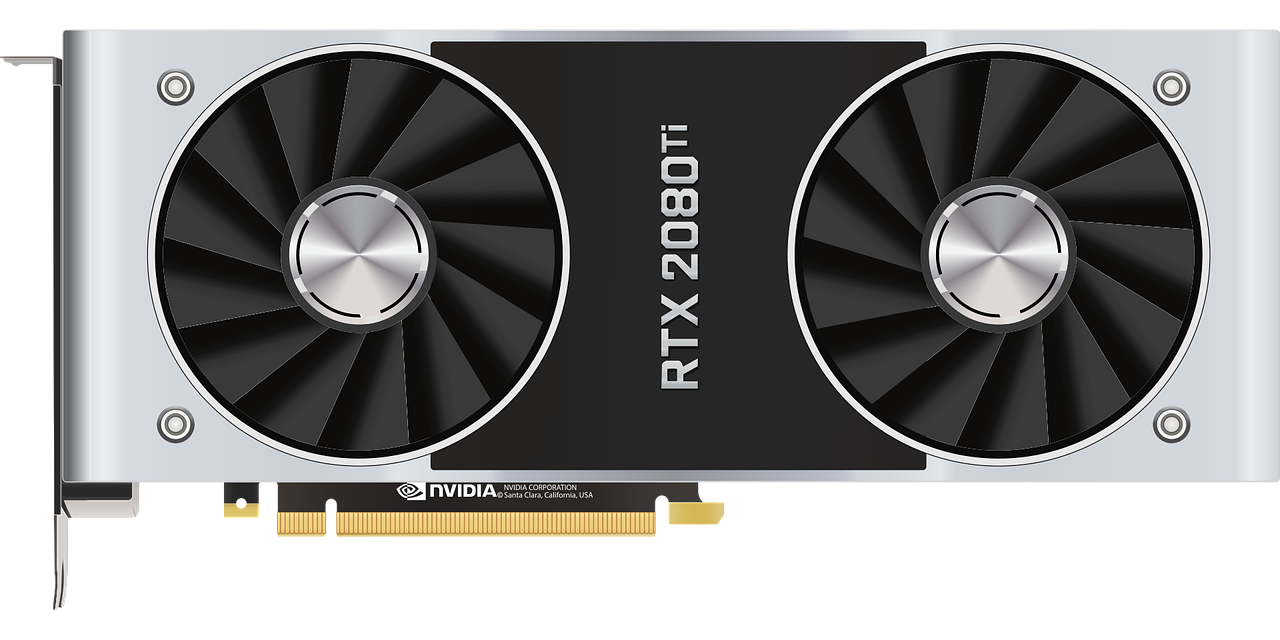
\includegraphics[width=0.6\linewidth]{img/nvidia_geeforce} \end{center}

Why did the hardware industry not simply invest in the development of more powerful CPUs to deal with the more demanding PC games? The main reason is that the architecture of CPUs is designed not only for efficiency but also flexibility. That is, a CPU needs to perform well in all kind of computations, some parallel, some sequential, etc. Computing graphics is a comparatively narrow domain of computation and designing a processing unit architecture that is custom-made to excel just at this one task is thus much more cost efficient. Interestingly, this graphics-specific architecture (specialized on highly parallel numerical {[}floating point{]} workloads) turns out to be also very useful in some core scientific computing tasks. In particular, matrix multiplications (see \citet{fatahalian_etal2004} for a detailed discussion of why that is the case). A key aspect of GPUs is that they are composed of several multiprocessor units, of which each has in turn several cores. GPUS thus can perform computations with hundreds or even thousands of threads in parallel. The figure below illustrates this point.

\begin{center}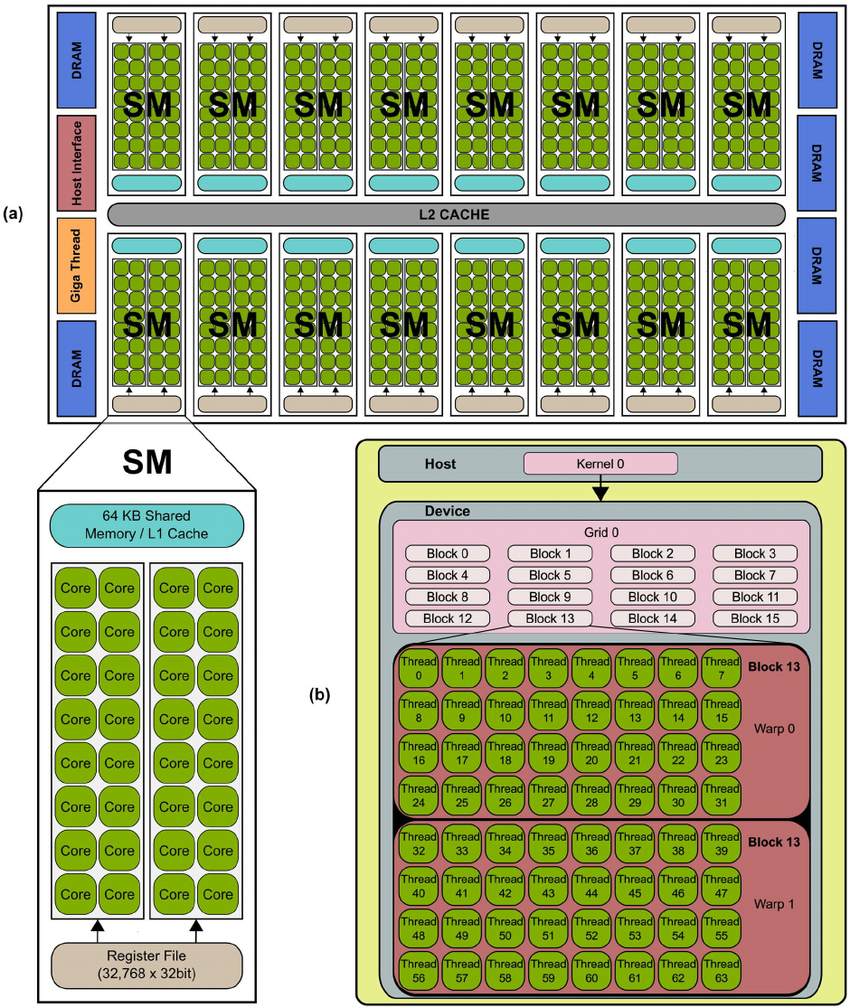
\includegraphics[width=0.6\linewidth]{img/nvidia_gpu} \end{center}

While, initially, programming GPUs for scientific computing required a very good understanding of the hardware. Graphics card producers have realized that there is an additional market for their products (in particular with the recent rise of deep learning), and provide several high-level APIs to use GPUs for other tasks than graphics processing. Over the last few years more high-level software has been developed, which makes it much easier to use GPUs in parallel computing tasks. The following subsections shows some examples of such software in the R environment.\footnote{Note that while these examples are easy to implement and run, setting up a GPU for scientific computing still can involve many steps and some knowledge of your computer's system. The examples presuppose that all installation and configuration steps (GPU drivers, CUDA, etc.) have already been completed successfully.}

\hypertarget{gpus-in-r}{%
\section{GPUs in R}\label{gpus-in-r}}

\hypertarget{example-i-matrix-multiplication-comparison-gpur}{%
\subsection{\texorpdfstring{Example I: Matrix multiplication comparison (\texttt{gpuR})}{Example I: Matrix multiplication comparison (gpuR)}}\label{example-i-matrix-multiplication-comparison-gpur}}

The \texttt{gpuR} package provides basic R functions to compute with GPUs from within the R environmnent. In the following example we compare the performance of the CPU with the GPU based on a matrix multiplication exercise. For a large \(N\times P\) matrix \(X\), we want to compute \(X^tX\).

In a first step, we load the \texttt{gpuR}-package.\footnote{As with the setting up of GPUs on your machine in general, installing all prerequisites to make \texttt{gpuR} work on your local machine can be a bit of work and can depend a lot on your system.} Note the output to the console. It shows the type of GPU identified by \texttt{gpuR}. This is the platform on which \texttt{gpuR} will compute the GPU examples. In order to compare the performances, we also load the \texttt{bench} package used in previous lectures.

\begin{Shaded}
\begin{Highlighting}[]
\CommentTok{\# load package}
\FunctionTok{library}\NormalTok{(bench)}
\FunctionTok{library}\NormalTok{(gpuR)}
\end{Highlighting}
\end{Shaded}

\begin{verbatim}
## Number of platforms: 1
## - platform: NVIDIA Corporation: OpenCL 3.0 CUDA 11.4.158
##   - context device index: 0
##     - NVIDIA GeForce GTX 1650
## checked all devices
## completed initialization
\end{verbatim}

Next, we initiate a large matrix filled with pseudo random numbers, representing a dataset with \(N\) observations and \(P\) variables.

\begin{Shaded}
\begin{Highlighting}[]
\CommentTok{\# initiate dataset with pseudo random numbers}
\NormalTok{N }\OtherTok{\textless{}{-}} \DecValTok{10000}  \CommentTok{\# number of observations}
\NormalTok{P }\OtherTok{\textless{}{-}} \DecValTok{100} \CommentTok{\# number of variables}
\NormalTok{X }\OtherTok{\textless{}{-}} \FunctionTok{matrix}\NormalTok{(}\FunctionTok{rnorm}\NormalTok{(N }\SpecialCharTok{*}\NormalTok{ P, }\DecValTok{0}\NormalTok{, }\DecValTok{1}\NormalTok{), }\AttributeTok{nrow =}\NormalTok{ N, }\AttributeTok{ncol =}\NormalTok{P)}
\end{Highlighting}
\end{Shaded}

For the GPU examples to work, we need one more preparatory step. GPUs have their own memory, which they can access faster than they can access RAM. However, this GPU memory is typically not very large compared to the memory CPUs have access to. Hence, there is a potential trade-off between losing some efficiency but working with more data or vice versa.\footnote{If we instruct the GPU to use the own memory, but the data does not fit in it, the program will result in an error.} Here, we show both variants. With \texttt{gpuMatrix()} we create an object representing matrix \texttt{X} for computation on the GPU. However, this only points the GPU to the matrix and does not actually transfer data to the GPU's memory. The latter is done in the other variant with \texttt{vclMatrix()}.

\begin{Shaded}
\begin{Highlighting}[]
\CommentTok{\# prepare GPU{-}specific objects/settings}
\NormalTok{gpuX }\OtherTok{\textless{}{-}} \FunctionTok{gpuMatrix}\NormalTok{(X, }\AttributeTok{type =} \StringTok{"float"}\NormalTok{)  }\CommentTok{\# point GPU to matrix (matrix stored in non{-}GPU memory)}
\NormalTok{vclX }\OtherTok{\textless{}{-}} \FunctionTok{vclMatrix}\NormalTok{(X, }\AttributeTok{type =} \StringTok{"float"}\NormalTok{)  }\CommentTok{\# transfer matrix to GPU (matrix stored in GPU memory)}
\end{Highlighting}
\end{Shaded}

Now we run the three examples: first, based on standard R, using the CPU. Then, computing on the GPU but using CPU memory. And finally, computing on the GPU and using GPU memory. In order to make the comparison fair, we force \texttt{bench::mark()} to run at least 20 iterations per benchmarked variant.

\begin{Shaded}
\begin{Highlighting}[]
\CommentTok{\# compare three approaches}
\NormalTok{(gpu\_cpu }\OtherTok{\textless{}{-}}\NormalTok{ bench}\SpecialCharTok{::}\FunctionTok{mark}\NormalTok{(}
  
  \CommentTok{\# compute with CPU }
\NormalTok{  cpu }\OtherTok{\textless{}{-}} \FunctionTok{t}\NormalTok{(X) }\SpecialCharTok{\%*\%}\NormalTok{ X,}
  
  \CommentTok{\# GPU version, GPU pointer to CPU memory (gpuMatrix is simply a pointer)}
\NormalTok{  gpu1\_pointer }\OtherTok{\textless{}{-}} \FunctionTok{t}\NormalTok{(gpuX) }\SpecialCharTok{\%*\%}\NormalTok{ gpuX,}
  
  \CommentTok{\# GPU version, in GPU memory (vclMatrix formation is a memory transfer)}
\NormalTok{  gpu2\_memory }\OtherTok{\textless{}{-}} \FunctionTok{t}\NormalTok{(vclX) }\SpecialCharTok{\%*\%}\NormalTok{ vclX,}
 
\AttributeTok{check =} \ConstantTok{FALSE}\NormalTok{, }\AttributeTok{memory =} \ConstantTok{FALSE}\NormalTok{, }\AttributeTok{min\_iterations =} \DecValTok{20}\NormalTok{))}
\end{Highlighting}
\end{Shaded}

\begin{verbatim}
## # A tibble: 3 x 6
##   expression                            min   median
##   <bch:expr>                       <bch:tm> <bch:tm>
## 1 cpu <- t(X) %*% X                 63.05ms   65.4ms
## 2 gpu1_pointer <- t(gpuX) %*% gpuX  27.24ms     29ms
## 3 gpu2_memory <- t(vclX) %*% vclX    6.98ms     14ms
## # ... with 3 more variables: itr/sec <dbl>,
## #   mem_alloc <bch:byt>, gc/sec <dbl>
\end{verbatim}

The performance comparison is visualized with boxplots.

\begin{Shaded}
\begin{Highlighting}[]
\FunctionTok{plot}\NormalTok{(gpu\_cpu, }\AttributeTok{type =} \StringTok{"boxplot"}\NormalTok{)}
\end{Highlighting}
\end{Shaded}

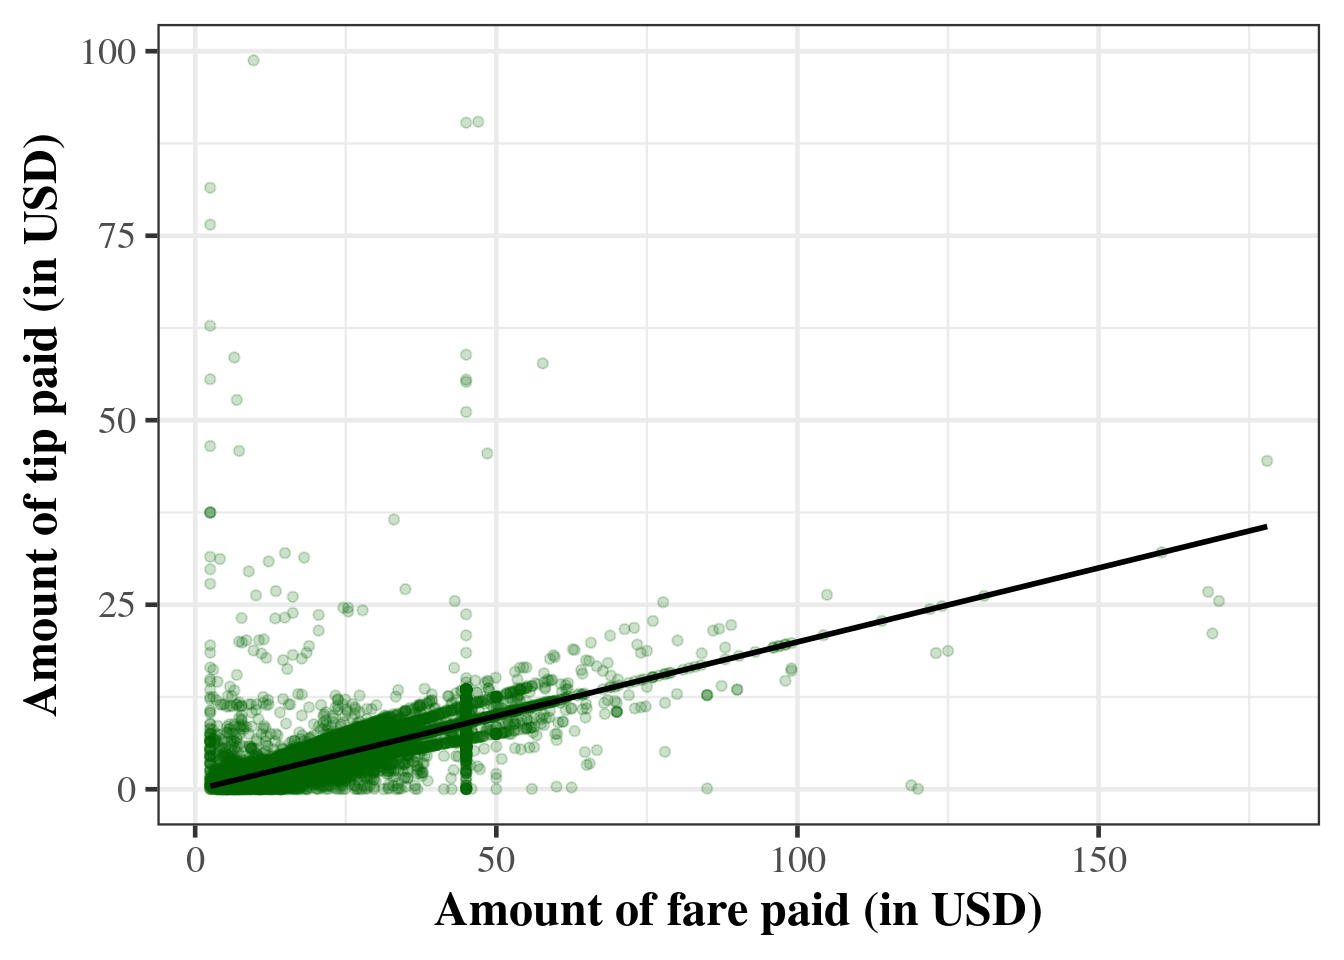
\includegraphics{bigdata_files/figure-latex/unnamed-chunk-195-1.pdf}

\hypertarget{gpus-and-machine-learning}{%
\section{GPUs and Machine Learning}\label{gpus-and-machine-learning}}

A most common application of GPUs for scientific computing is machine learning, in particular deep learning (machine learning based on artificial neural networks). Training deep learning models can be very computationally intense and to an important part depends on tensor (matrix) multiplications. This is also an area where you might come across highly parallelized computing based on GPUs without even noticing it, as the now commonly used software to build and train deep neural nets (\href{https://www.tensorflow.org/}{tensorflow}, and the high-level \href{https://keras.io/}{Keras} API) can easily be run on a CPU or GPU without any further configuration/preparation (apart from the initial installation of these programs). The example below is a simple illustration of how such techniques can be used in an econometrics context.

\hypertarget{tensorflowkeras-example-predict-housing-prices}{%
\subsection{Tensorflow/Keras example: predict housing prices}\label{tensorflowkeras-example-predict-housing-prices}}

In this example we train a simple sequential model with two hidden layers in order to predict the median value of owner-occupied homes (in USD 1,000) in the Boston area (data are from the 1970s). The original data and a detailed description can be found \href{https://www.cs.toronto.edu/~delve/data/boston/bostonDetail.html}{here}. The example follows closely \href{https://keras.rstudio.com/articles/tutorial_basic_regression.html\#the-boston-housing-prices-dataset}{this keras tutorial} published by RStudio. See \href{https://keras.rstudio.com/index.html}{RStudio's keras installation guide} for how to install keras (and tensorflow) and the corresponding R package \texttt{keras}.\footnote{This might involve the installation of additional packages and software outside the R environment.} While the purpose of the example here is to demonstrate a typical (but very simple!) usage case of GPUs in machine learning, the same code should also run on a normal machine (without using GPUs) with a default installation of keras.

Apart from \texttt{keras}, we load packages to prepare the data and visualize the output. Via \texttt{dataset\_boston\_housing()}, we load the dataset (shipped with the keras installation) in the format preferred by the \texttt{keras} library.

\begin{Shaded}
\begin{Highlighting}[]
\CommentTok{\# load packages}
\FunctionTok{library}\NormalTok{(keras)}
\FunctionTok{library}\NormalTok{(tibble)}
\FunctionTok{library}\NormalTok{(ggplot2)}
\FunctionTok{library}\NormalTok{(tfdatasets)}


\CommentTok{\# load data}
\NormalTok{boston\_housing }\OtherTok{\textless{}{-}} \FunctionTok{dataset\_boston\_housing}\NormalTok{()}
\FunctionTok{str}\NormalTok{(boston\_housing)}
\end{Highlighting}
\end{Shaded}

\begin{verbatim}
## List of 2
##  $ train:List of 2
##   ..$ x: num [1:404, 1:13] 1.2325 0.0218 4.8982 0.0396 3.6931 ...
##   ..$ y: num [1:404(1d)] 15.2 42.3 50 21.1 17.7 18.5 11.3 15.6 15.6 14.4 ...
##  $ test :List of 2
##   ..$ x: num [1:102, 1:13] 18.0846 0.1233 0.055 1.2735 0.0715 ...
##   ..$ y: num [1:102(1d)] 7.2 18.8 19 27 22.2 24.5 31.2 22.9 20.5 23.2 ...
\end{verbatim}

In a first step, we split the data into a training set and a test set. The latter is used to monitor the out-of-sample performance of the model fit. Testing the validity of an estimated model by looking at how it performs out-of-sample is of particular relevance when working with (deep) neural networks, as they can easily lead to over-fitting. Validity checks based on the test sample are, therefore, often an integral part of modelling with tensorflow/keras.

\begin{Shaded}
\begin{Highlighting}[]
\CommentTok{\# assign training and test data/labels}
\FunctionTok{c}\NormalTok{(train\_data, train\_labels) }\SpecialCharTok{\%\textless{}{-}\%}\NormalTok{ boston\_housing}\SpecialCharTok{$}\NormalTok{train}
\FunctionTok{c}\NormalTok{(test\_data, test\_labels) }\SpecialCharTok{\%\textless{}{-}\%}\NormalTok{ boston\_housing}\SpecialCharTok{$}\NormalTok{test}
\end{Highlighting}
\end{Shaded}

In order to better understand and interpret the dataset we add the original variable names, and convert it to a \texttt{tibble}.

\begin{Shaded}
\begin{Highlighting}[]
\FunctionTok{library}\NormalTok{(dplyr)}

\NormalTok{column\_names }\OtherTok{\textless{}{-}} \FunctionTok{c}\NormalTok{(}\StringTok{\textquotesingle{}CRIM\textquotesingle{}}\NormalTok{, }\StringTok{\textquotesingle{}ZN\textquotesingle{}}\NormalTok{, }\StringTok{\textquotesingle{}INDUS\textquotesingle{}}\NormalTok{, }\StringTok{\textquotesingle{}CHAS\textquotesingle{}}\NormalTok{, }\StringTok{\textquotesingle{}NOX\textquotesingle{}}\NormalTok{, }\StringTok{\textquotesingle{}RM\textquotesingle{}}\NormalTok{, }\StringTok{\textquotesingle{}AGE\textquotesingle{}}\NormalTok{, }
                  \StringTok{\textquotesingle{}DIS\textquotesingle{}}\NormalTok{, }\StringTok{\textquotesingle{}RAD\textquotesingle{}}\NormalTok{, }\StringTok{\textquotesingle{}TAX\textquotesingle{}}\NormalTok{, }\StringTok{\textquotesingle{}PTRATIO\textquotesingle{}}\NormalTok{, }\StringTok{\textquotesingle{}B\textquotesingle{}}\NormalTok{, }\StringTok{\textquotesingle{}LSTAT\textquotesingle{}}\NormalTok{)}

\NormalTok{train\_df }\OtherTok{\textless{}{-}}\NormalTok{ train\_data }\SpecialCharTok{\%\textgreater{}\%} 
  \FunctionTok{as\_tibble}\NormalTok{(}\AttributeTok{.name\_repair =} \StringTok{"minimal"}\NormalTok{) }\SpecialCharTok{\%\textgreater{}\%} 
  \FunctionTok{setNames}\NormalTok{(column\_names) }\SpecialCharTok{\%\textgreater{}\%} 
  \FunctionTok{mutate}\NormalTok{(}\AttributeTok{label =}\NormalTok{ train\_labels)}

\NormalTok{test\_df }\OtherTok{\textless{}{-}}\NormalTok{ test\_data }\SpecialCharTok{\%\textgreater{}\%} 
  \FunctionTok{as\_tibble}\NormalTok{(}\AttributeTok{.name\_repair =} \StringTok{"minimal"}\NormalTok{) }\SpecialCharTok{\%\textgreater{}\%} 
  \FunctionTok{setNames}\NormalTok{(column\_names) }\SpecialCharTok{\%\textgreater{}\%} 
  \FunctionTok{mutate}\NormalTok{(}\AttributeTok{label =}\NormalTok{ test\_labels)}
\end{Highlighting}
\end{Shaded}

Next, we have a close look at the data. Note the usage of the term `label' for what is usually called the `dependent variable' in econometrics.\footnote{Typical textbook examples in machine learning deal with classification (e.g.~a logit model), while in microeconometrics the typical example is usually a linear model (continuous dependent variable).} As the aim of the exercise is to predict median prices of homes, the output of the model will be a continuous value (`labels').

\begin{Shaded}
\begin{Highlighting}[]
\CommentTok{\# check example data dimensions and content}
\FunctionTok{paste0}\NormalTok{(}\StringTok{"Training entries: "}\NormalTok{, }\FunctionTok{length}\NormalTok{(train\_data), }\StringTok{", labels: "}\NormalTok{, }\FunctionTok{length}\NormalTok{(train\_labels))}
\end{Highlighting}
\end{Shaded}

\begin{verbatim}
## [1] "Training entries: 5252, labels: 404"
\end{verbatim}

\begin{Shaded}
\begin{Highlighting}[]
\FunctionTok{summary}\NormalTok{(train\_data)}
\end{Highlighting}
\end{Shaded}

\begin{verbatim}
##        V1              V2              V3       
##  Min.   : 0.01   Min.   :  0.0   Min.   : 0.46  
##  1st Qu.: 0.08   1st Qu.:  0.0   1st Qu.: 5.13  
##  Median : 0.27   Median :  0.0   Median : 9.69  
##  Mean   : 3.75   Mean   : 11.5   Mean   :11.10  
##  3rd Qu.: 3.67   3rd Qu.: 12.5   3rd Qu.:18.10  
##  Max.   :88.98   Max.   :100.0   Max.   :27.74  
##        V4               V5              V6      
##  Min.   :0.0000   Min.   :0.385   Min.   :3.56  
##  1st Qu.:0.0000   1st Qu.:0.453   1st Qu.:5.88  
##  Median :0.0000   Median :0.538   Median :6.20  
##  Mean   :0.0619   Mean   :0.557   Mean   :6.27  
##  3rd Qu.:0.0000   3rd Qu.:0.631   3rd Qu.:6.61  
##  Max.   :1.0000   Max.   :0.871   Max.   :8.72  
##        V7              V8              V9       
##  Min.   :  2.9   Min.   : 1.13   Min.   : 1.00  
##  1st Qu.: 45.5   1st Qu.: 2.08   1st Qu.: 4.00  
##  Median : 78.5   Median : 3.14   Median : 5.00  
##  Mean   : 69.0   Mean   : 3.74   Mean   : 9.44  
##  3rd Qu.: 94.1   3rd Qu.: 5.12   3rd Qu.:24.00  
##  Max.   :100.0   Max.   :10.71   Max.   :24.00  
##       V10           V11            V12       
##  Min.   :188   Min.   :12.6   Min.   :  0.3  
##  1st Qu.:279   1st Qu.:17.2   1st Qu.:374.7  
##  Median :330   Median :19.1   Median :391.2  
##  Mean   :406   Mean   :18.5   Mean   :354.8  
##  3rd Qu.:666   3rd Qu.:20.2   3rd Qu.:396.2  
##  Max.   :711   Max.   :22.0   Max.   :396.9  
##       V13       
##  Min.   : 1.73  
##  1st Qu.: 6.89  
##  Median :11.39  
##  Mean   :12.74  
##  3rd Qu.:17.09  
##  Max.   :37.97
\end{verbatim}

\begin{Shaded}
\begin{Highlighting}[]
\FunctionTok{summary}\NormalTok{(train\_labels) }\CommentTok{\# Display first 10 entries}
\end{Highlighting}
\end{Shaded}

\begin{verbatim}
##    Min. 1st Qu.  Median    Mean 3rd Qu.    Max. 
##     5.0    16.7    20.8    22.4    24.8    50.0
\end{verbatim}

As the dataset contains variables ranging from per capita crime rate to indicators for highway access, the variables are obviously measured in different units and hence displayed on different scales. This is not per se a problem for the fitting procedure. However, fitting is more efficient when all features (variables) are normalized.

\begin{Shaded}
\begin{Highlighting}[]
\NormalTok{spec }\OtherTok{\textless{}{-}} \FunctionTok{feature\_spec}\NormalTok{(train\_df, label }\SpecialCharTok{\textasciitilde{}}\NormalTok{ . ) }\SpecialCharTok{\%\textgreater{}\%} 
  \FunctionTok{step\_numeric\_column}\NormalTok{(}\FunctionTok{all\_numeric}\NormalTok{(), }\AttributeTok{normalizer\_fn =} \FunctionTok{scaler\_standard}\NormalTok{()) }\SpecialCharTok{\%\textgreater{}\%} 
  \FunctionTok{fit}\NormalTok{()}

\NormalTok{layer }\OtherTok{\textless{}{-}} \FunctionTok{layer\_dense\_features}\NormalTok{(}
  \AttributeTok{feature\_columns =} \FunctionTok{dense\_features}\NormalTok{(spec), }
  \AttributeTok{dtype =}\NormalTok{ tf}\SpecialCharTok{$}\NormalTok{float32}
\NormalTok{)}
\FunctionTok{layer}\NormalTok{(train\_df)}
\end{Highlighting}
\end{Shaded}

\begin{verbatim}
## tf.Tensor(
## [[ 0.81205493  0.44752213 -0.2565147  ... -0.1762239  -0.59443307
##   -0.48301655]
##  [-1.9079947   0.43137115 -0.2565147  ...  1.8920003  -0.34800112
##    2.9880793 ]
##  [ 1.1091131   0.2203439  -0.2565147  ... -1.8274226   1.563349
##   -0.48301655]
##  ...
##  [-1.6359899   0.07934052 -0.2565147  ... -0.3326088  -0.61246467
##    0.9895695 ]
##  [ 1.0554279  -0.98642045 -0.2565147  ... -0.7862657  -0.01742171
##   -0.48301655]
##  [-1.7970455   0.23288251 -0.2565147  ...  0.47467488 -0.84687555
##    2.0414166 ]], shape=(404, 13), dtype=float32)
\end{verbatim}

We specify the model as a linear stack of layers: The input (all 13 explanatory variables), two densely connected hidden layers (each with a 64-dimensional output space), and finally the one-dimensional output layer (the `dependent variable').

\begin{Shaded}
\begin{Highlighting}[]
\CommentTok{\# Create the model}
\CommentTok{\# model specification}
\NormalTok{input }\OtherTok{\textless{}{-}} \FunctionTok{layer\_input\_from\_dataset}\NormalTok{(train\_df }\SpecialCharTok{\%\textgreater{}\%} \FunctionTok{select}\NormalTok{(}\SpecialCharTok{{-}}\NormalTok{label))}

\NormalTok{output }\OtherTok{\textless{}{-}}\NormalTok{ input }\SpecialCharTok{\%\textgreater{}\%} 
  \FunctionTok{layer\_dense\_features}\NormalTok{(}\FunctionTok{dense\_features}\NormalTok{(spec)) }\SpecialCharTok{\%\textgreater{}\%} 
  \FunctionTok{layer\_dense}\NormalTok{(}\AttributeTok{units =} \DecValTok{64}\NormalTok{, }\AttributeTok{activation =} \StringTok{"relu"}\NormalTok{) }\SpecialCharTok{\%\textgreater{}\%}
  \FunctionTok{layer\_dense}\NormalTok{(}\AttributeTok{units =} \DecValTok{64}\NormalTok{, }\AttributeTok{activation =} \StringTok{"relu"}\NormalTok{) }\SpecialCharTok{\%\textgreater{}\%}
  \FunctionTok{layer\_dense}\NormalTok{(}\AttributeTok{units =} \DecValTok{1}\NormalTok{) }

\NormalTok{model }\OtherTok{\textless{}{-}} \FunctionTok{keras\_model}\NormalTok{(input, output)}
\end{Highlighting}
\end{Shaded}

In order to fit the model, we first have to compile it (configure it for training). At this step we set the configuration parameters that will guide the training/optimization procedure. We use the mean squared errors loss function (\texttt{mse}) typically used for regressions. We chose the \href{http://www.cs.toronto.edu/~tijmen/csc321/slides/lecture_slides_lec6.pdf}{RMSProp} optimizer to find the minimum loss.

\begin{Shaded}
\begin{Highlighting}[]
\CommentTok{\# compile the model  }
\NormalTok{model }\SpecialCharTok{\%\textgreater{}\%} 
  \FunctionTok{compile}\NormalTok{(}
    \AttributeTok{loss =} \StringTok{"mse"}\NormalTok{,}
    \AttributeTok{optimizer =} \FunctionTok{optimizer\_rmsprop}\NormalTok{(),}
    \AttributeTok{metrics =} \FunctionTok{list}\NormalTok{(}\StringTok{"mean\_absolute\_error"}\NormalTok{)}
\NormalTok{  )}
\end{Highlighting}
\end{Shaded}

Now we can get a summary of the model we are about to fit to the data.

\begin{Shaded}
\begin{Highlighting}[]
\CommentTok{\# get a summary of the model}
\NormalTok{model}
\end{Highlighting}
\end{Shaded}

\begin{verbatim}
## Model
## Model: "model"
## _______________________________________________________
## Layer (type)      Output Shap Param Connected to       
## =======================================================
## AGE (InputLayer)  [(None,)]   0                        
## _______________________________________________________
## B (InputLayer)    [(None,)]   0                        
## _______________________________________________________
## CHAS (InputLayer) [(None,)]   0                        
## _______________________________________________________
## CRIM (InputLayer) [(None,)]   0                        
## _______________________________________________________
## DIS (InputLayer)  [(None,)]   0                        
## _______________________________________________________
## INDUS (InputLayer [(None,)]   0                        
## _______________________________________________________
## LSTAT (InputLayer [(None,)]   0                        
## _______________________________________________________
## NOX (InputLayer)  [(None,)]   0                        
## _______________________________________________________
## PTRATIO (InputLay [(None,)]   0                        
## _______________________________________________________
## RAD (InputLayer)  [(None,)]   0                        
## _______________________________________________________
## RM (InputLayer)   [(None,)]   0                        
## _______________________________________________________
## TAX (InputLayer)  [(None,)]   0                        
## _______________________________________________________
## ZN (InputLayer)   [(None,)]   0                        
## _______________________________________________________
## dense_features_1  (None, 13)  0     AGE[0][0]          
##                                     B[0][0]            
##                                     CHAS[0][0]         
##                                     CRIM[0][0]         
##                                     DIS[0][0]          
##                                     INDUS[0][0]        
##                                     LSTAT[0][0]        
##                                     NOX[0][0]          
##                                     PTRATIO[0][0]      
##                                     RAD[0][0]          
##                                     RM[0][0]           
##                                     TAX[0][0]          
##                                     ZN[0][0]           
## _______________________________________________________
## dense_2 (Dense)   (None, 64)  896   dense_features_1[0]
## _______________________________________________________
## dense_1 (Dense)   (None, 64)  4160  dense_2[0][0]      
## _______________________________________________________
## dense (Dense)     (None, 1)   65    dense_1[0][0]      
## =======================================================
## Total params: 5,121
## Trainable params: 5,121
## Non-trainable params: 0
## _______________________________________________________
\end{verbatim}

Given the relatively simple model and small dataset, we set the maximum number of epochs to 500 and allow for early stopping in case the validation loss (based on test data) is not improving for a while.

\begin{Shaded}
\begin{Highlighting}[]
\CommentTok{\# Set max. number of epochs}
\NormalTok{epochs }\OtherTok{\textless{}{-}} \DecValTok{500}
\end{Highlighting}
\end{Shaded}

Finally, we fit the model while preserving the training history, and visualize the training progress.

\begin{Shaded}
\begin{Highlighting}[]
\CommentTok{\# Fit the model and store training stats}

\NormalTok{history }\OtherTok{\textless{}{-}}\NormalTok{ model }\SpecialCharTok{\%\textgreater{}\%} \FunctionTok{fit}\NormalTok{(}
  \AttributeTok{x =}\NormalTok{ train\_df }\SpecialCharTok{\%\textgreater{}\%} \FunctionTok{select}\NormalTok{(}\SpecialCharTok{{-}}\NormalTok{label),}
  \AttributeTok{y =}\NormalTok{ train\_df}\SpecialCharTok{$}\NormalTok{label,}
  \AttributeTok{epochs =}\NormalTok{ epochs,}
  \AttributeTok{validation\_split =} \FloatTok{0.2}\NormalTok{,}
  \AttributeTok{verbose =} \DecValTok{0}
\NormalTok{)}


\FunctionTok{plot}\NormalTok{(history)}
\end{Highlighting}
\end{Shaded}

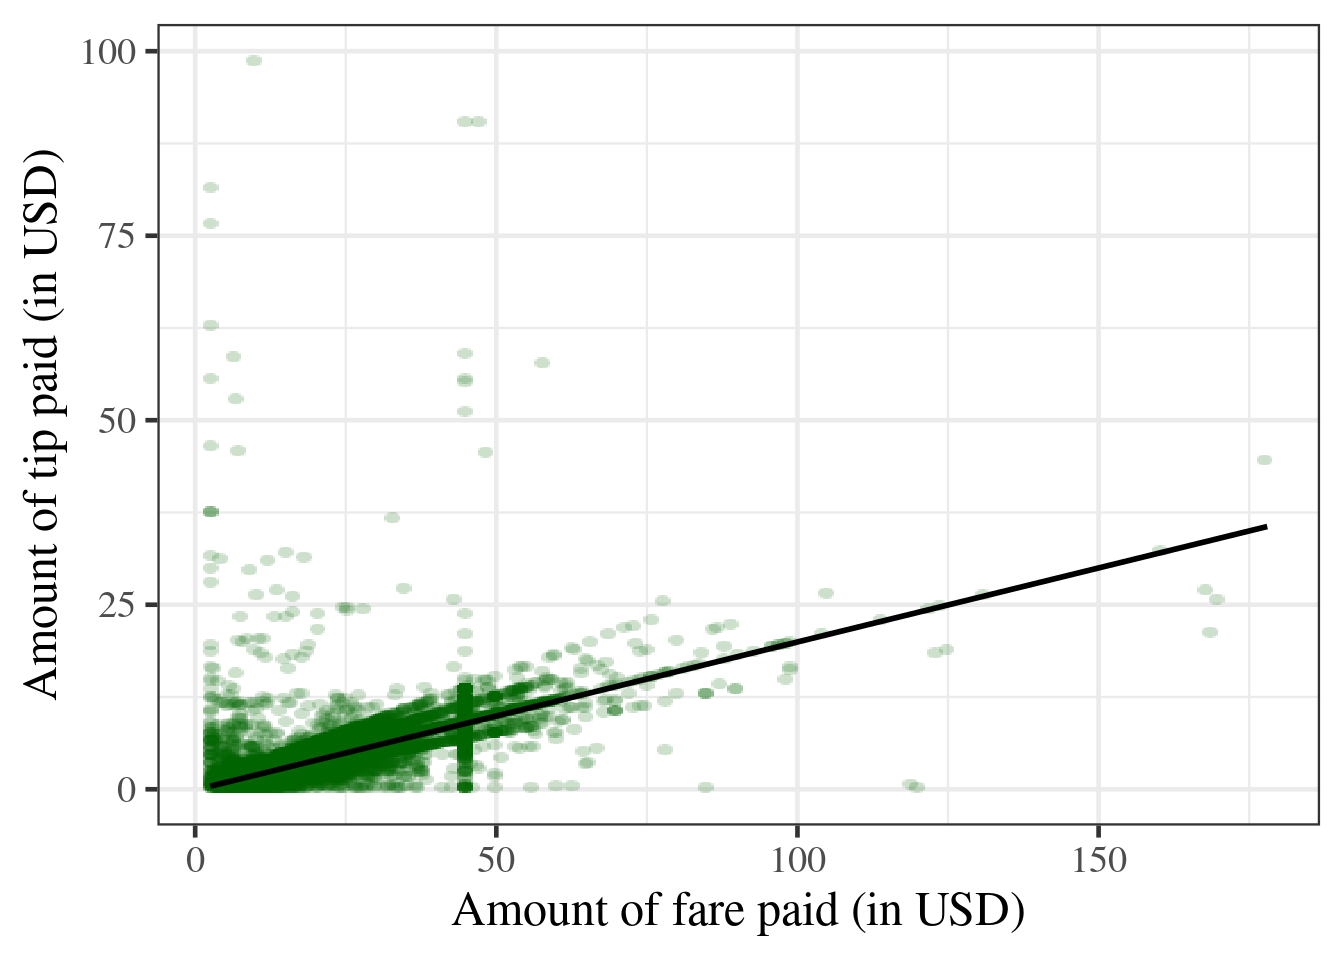
\includegraphics{bigdata_files/figure-latex/unnamed-chunk-206-1.pdf}

\hypertarget{a-word-of-caution}{%
\section{A word of caution}\label{a-word-of-caution}}

From just comparing the number of threads of a modern CPU with the number of threads of a modern GPU, one might get the impression that parallel tasks should always be implemented for GPU computing. However, whether one approach or the other is faster can depend a lot on the overall task and the data at hand. Moreover, the parallel implementation of tasks can be done more or less well on either system. Really efficient parallel implementation of tasks can take a lot of coding time (particularly when done for GPUs).\footnote{For a more detailed discussion of the relevant factors for well done parallelization (either on CPUs or GPUs), see \citet{matloff_2015}}.

\hypertarget{applied-econometrics-with-apache-spark}{%
\chapter{Applied Econometrics with Apache Spark}\label{applied-econometrics-with-apache-spark}}

\hypertarget{spark-basics}{%
\section{Spark basics}\label{spark-basics}}

Building on the MapReduce model discussed in the previous lecture, \href{https://spark.apache.org/}{Apache Spark} is a cluster computing platform particularly made for data analytics. From the technical perspective (in very simple terms), Spark improves some shortcomings of the older \href{https://hadoop.apache.org/}{Hadoop} platform, further improving efficiency/speed. More importantly for our purposes, in contrast to Hadoop, Spark is specifically made for analytics tasks and therefore more easily accessible for people with an applied econometrics background but no substantial knowledge in MapReduce cluster computing. In particular, it comes with several high-level operators that make it rather easy to implement analytics tasks. Moreover (in contrast to basic Hadoop), its very easy to use interactively from R, Python, Scala, and SQL. This makes the platform much more accessible and worth the while for empirical economic research, even for relatively simple econometric analyses.

The following figure illustrates the basic components of Spark. The main functionality, including memory management, task scheduling, and the implementation of Spark's capabilities to handle and manipulate data distributed across many nodes in parallel. Several built-in libraries extend the core implementation, covering specific domains of practical data analytics tasks (querying structured data via SQL, processing streams of data, machine learning, and network/graph analysis). The latter two provide various common functions/algorithms frequently used in data analytics/applied econometrics, such as generalized linear regression, summary statistics, and principal component analysis.

\begin{figure}

{\centering 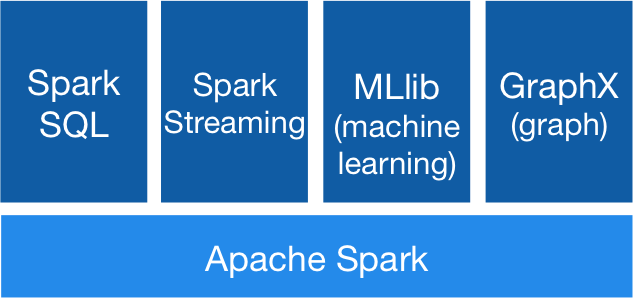
\includegraphics[width=0.6\linewidth]{img/spark-stack} 

}

\caption{Basic Spark stack (source: \url{https://spark.apache.org/images/spark-stack.png})}\label{fig:sparkstack}
\end{figure}



At the heart of big data analytics with Spark is the fundamental data structure called `resilient distributed dataset' (RDD). When loading/importing data into Spark, the data is automatically distributed across the cluster in RDDs (\textasciitilde{} as distributed collections of elements) and manipulations are then executed in parallel in these RDDs. However, the entire Spark framework also works locally on a simple laptop or desktop computer. This is of great advantage when learning Spark and testing/debugging an analytics script on a small sample of the real dataset.

\hypertarget{spark-in-r}{%
\section{Spark in R}\label{spark-in-r}}

There are two prominent packages to use Spark in connection to R: \texttt{SparkR} and RStudio's \texttt{sparklyr}, the former is in some ways closer to Spark's Python API, the latter is closer to the \texttt{dplyr}-type of data handling (and is `compatible' with the `\texttt{tidyverse}').\footnote{See \href{https://cosminsanda.com/posts/a-compelling-case-for-sparkr/}{this blog post} for a more detailed comparison and discussion of advantages of either package.} For the very simple introductory examples below, either package could have been used equally well. For the general introduction we focus on \texttt{SparkR} and later have a look at a simple regression example based on \texttt{sparklyr}.

To install and use Spark from the R shell, only a few preparatory steps are needed. The following examples are based on installing/running Spark on a Linux machine with the \texttt{SparkR} package. \texttt{SparkR} depends on Java (version 8). Thus, we first should make sure the right Java version is installed. If several Java versions are installed, we might have to select version 8 manually via the following terminal command (Linux).

With the right version of Java running, we can install \texttt{SparkR} as usual with \texttt{install.packages("SparkR")}. After installing \texttt{SparkR}, the call \texttt{SparkR::install.spark()} will download and install Apache Spark to a local directory. No we can start an interactive Spark session from within R.

\begin{Shaded}
\begin{Highlighting}[]
\CommentTok{\# install.packages("SparkR")}
\CommentTok{\# or, if temporarily not available on CRAN:}
\CommentTok{\#if (!require(\textquotesingle{}devtools\textquotesingle{})) install.packages(\textquotesingle{}devtools\textquotesingle{})}
\CommentTok{\#devtools::install\_github(\textquotesingle{}apache/spark@v2.x.x\textquotesingle{}, subdir=\textquotesingle{}R/pkg\textquotesingle{}) \# replace x.x with the version of your spark installation}

\CommentTok{\# load packages}
\FunctionTok{library}\NormalTok{(SparkR)}

\CommentTok{\# start session}
\FunctionTok{sparkR.session}\NormalTok{()}
\end{Highlighting}
\end{Shaded}

By default this starts a local standalone session (no connection to a cluster computer needed). While the examples below are all intended to run on a local machine, it is straightforward to connect to a remote Spark cluster and run the same examples there.\footnote{Simply set the \texttt{master} argument of \texttt{sparkR.session()} to the URL of the Spark master node of the remote cluster. Importantly, the local Spark and Hadoop versions should match the corresponding versions on the remote cluster.}

\hypertarget{data-import-and-summary-statistics}{%
\subsection{Data import and summary statistics}\label{data-import-and-summary-statistics}}

First, we want to have a brief look at how to perform the first few steps of a typical econometric analysis: import data and compute summary statistics. We analyze the already familiar \texttt{flights.csv} dataset. The basic Spark installation provides direct support to import common data formats such as CSV and JSON via the \texttt{read.df()} function (for many additional formats, specific Spark libraries are available). To import\texttt{flights.csv}, we set the \texttt{source}-argument to \texttt{"csv"}.

\begin{Shaded}
\begin{Highlighting}[]
\CommentTok{\# Import data and create a SparkDataFrame (a distributed collection of data, RDD)}
\NormalTok{flights }\OtherTok{\textless{}{-}} \FunctionTok{read.df}\NormalTok{(}\AttributeTok{path=}\StringTok{"data/flights.csv"}\NormalTok{, }\AttributeTok{source =} \StringTok{"csv"}\NormalTok{, }\AttributeTok{header=}\StringTok{"true"}\NormalTok{)}


\CommentTok{\# inspect the object}
\FunctionTok{class}\NormalTok{(flights)}
\end{Highlighting}
\end{Shaded}

\begin{verbatim}
## [1] "SparkDataFrame"
## attr(,"package")
## [1] "SparkR"
\end{verbatim}

\begin{Shaded}
\begin{Highlighting}[]
\FunctionTok{head}\NormalTok{(flights)}
\end{Highlighting}
\end{Shaded}

\begin{verbatim}
##   year month day dep_time sched_dep_time dep_delay
## 1 2013     1   1      517            515         2
## 2 2013     1   1      533            529         4
## 3 2013     1   1      542            540         2
## 4 2013     1   1      544            545        -1
## 5 2013     1   1      554            600        -6
## 6 2013     1   1      554            558        -4
##   arr_time sched_arr_time arr_delay carrier flight
## 1      830            819        11      UA   1545
## 2      850            830        20      UA   1714
## 3      923            850        33      AA   1141
## 4     1004           1022       -18      B6    725
## 5      812            837       -25      DL    461
## 6      740            728        12      UA   1696
##   tailnum origin dest air_time distance hour minute
## 1  N14228    EWR  IAH      227     1400    5     15
## 2  N24211    LGA  IAH      227     1416    5     29
## 3  N619AA    JFK  MIA      160     1089    5     40
## 4  N804JB    JFK  BQN      183     1576    5     45
## 5  N668DN    LGA  ATL      116      762    6      0
## 6  N39463    EWR  ORD      150      719    5     58
##              time_hour
## 1 2013-01-01T10:00:00Z
## 2 2013-01-01T10:00:00Z
## 3 2013-01-01T10:00:00Z
## 4 2013-01-01T10:00:00Z
## 5 2013-01-01T11:00:00Z
## 6 2013-01-01T10:00:00Z
\end{verbatim}

By default, all variables have been imported as type \texttt{character}. For several variables this is, of course, not the optimal data type to compute summary statistics. We thus first have to convert some columns to other data types with the \texttt{cast} function.

\begin{Shaded}
\begin{Highlighting}[]
\NormalTok{flights}\SpecialCharTok{$}\NormalTok{dep\_delay }\OtherTok{\textless{}{-}} \FunctionTok{cast}\NormalTok{(flights}\SpecialCharTok{$}\NormalTok{dep\_delay, }\StringTok{"double"}\NormalTok{)}
\NormalTok{flights}\SpecialCharTok{$}\NormalTok{dep\_time }\OtherTok{\textless{}{-}} \FunctionTok{cast}\NormalTok{(flights}\SpecialCharTok{$}\NormalTok{dep\_time, }\StringTok{"double"}\NormalTok{)}
\NormalTok{flights}\SpecialCharTok{$}\NormalTok{arr\_time }\OtherTok{\textless{}{-}} \FunctionTok{cast}\NormalTok{(flights}\SpecialCharTok{$}\NormalTok{arr\_time, }\StringTok{"double"}\NormalTok{)}
\NormalTok{flights}\SpecialCharTok{$}\NormalTok{arr\_delay }\OtherTok{\textless{}{-}} \FunctionTok{cast}\NormalTok{(flights}\SpecialCharTok{$}\NormalTok{arr\_delay, }\StringTok{"double"}\NormalTok{)}
\NormalTok{flights}\SpecialCharTok{$}\NormalTok{air\_time }\OtherTok{\textless{}{-}} \FunctionTok{cast}\NormalTok{(flights}\SpecialCharTok{$}\NormalTok{air\_time, }\StringTok{"double"}\NormalTok{)}
\NormalTok{flights}\SpecialCharTok{$}\NormalTok{distance }\OtherTok{\textless{}{-}} \FunctionTok{cast}\NormalTok{(flights}\SpecialCharTok{$}\NormalTok{distance, }\StringTok{"double"}\NormalTok{)}
\end{Highlighting}
\end{Shaded}

Suppose we only want to compute average arrival delays per carrier for flights with a distance over 1000 miles. Variable selection and filtering of observations is implemented in \texttt{select()} and \texttt{filter()} (as in the \texttt{dplyr} package).

\begin{Shaded}
\begin{Highlighting}[]
\CommentTok{\# filter}
\NormalTok{long\_flights }\OtherTok{\textless{}{-}} \FunctionTok{select}\NormalTok{(flights, }\StringTok{"carrier"}\NormalTok{, }\StringTok{"year"}\NormalTok{, }\StringTok{"arr\_delay"}\NormalTok{, }\StringTok{"distance"}\NormalTok{)}
\NormalTok{long\_flights }\OtherTok{\textless{}{-}} \FunctionTok{filter}\NormalTok{(long\_flights, long\_flights}\SpecialCharTok{$}\NormalTok{distance }\SpecialCharTok{\textgreater{}=} \DecValTok{1000}\NormalTok{)}
\FunctionTok{head}\NormalTok{(long\_flights)}
\end{Highlighting}
\end{Shaded}

\begin{verbatim}
##   carrier year arr_delay distance
## 1      UA 2013        11     1400
## 2      UA 2013        20     1416
## 3      AA 2013        33     1089
## 4      B6 2013       -18     1576
## 5      B6 2013        19     1065
## 6      B6 2013        -2     1028
\end{verbatim}

Now we summarize the arrival delays for the subset of long flights by carrier. This is the `split-apply-combine' approach applied in \texttt{SparkR}.

\begin{Shaded}
\begin{Highlighting}[]
\CommentTok{\# aggregation: mean delay per carrier}
\NormalTok{long\_flights\_delays}\OtherTok{\textless{}{-}} \FunctionTok{summarize}\NormalTok{(}\FunctionTok{groupBy}\NormalTok{(long\_flights, long\_flights}\SpecialCharTok{$}\NormalTok{carrier),}
                      \AttributeTok{avg\_delay =} \FunctionTok{mean}\NormalTok{(long\_flights}\SpecialCharTok{$}\NormalTok{arr\_delay))}
\FunctionTok{head}\NormalTok{(long\_flights\_delays)}
\end{Highlighting}
\end{Shaded}

\begin{verbatim}
##   carrier avg_delay
## 1      UA    3.2622
## 2      AA    0.4958
## 3      EV   15.6876
## 4      B6    9.0364
## 5      DL   -0.2394
## 6      OO   -2.0000
\end{verbatim}

Finally, we want to convert the result back into a usual \texttt{data.frame} (loaded in our current R session) in order to further process the summary statistics (output to LaTex table, plot, etc.). Note that as in the previous aggregation exercises with the \texttt{ff} package, the computed summary statistics (in the form of a table/df) are obviously much smaller than the raw data. However, note that converting a \texttt{SparkDataFrame} back into a native R object generally means all the data stored in the RDDs constituting the \texttt{SparkDataFrame} object are loaded into local RAM. Hence, when working with actual big data on a Spark cluster, this type of operation can quickly overflow local RAM.

\begin{Shaded}
\begin{Highlighting}[]
\CommentTok{\# Convert result back into native R object}
\NormalTok{delays }\OtherTok{\textless{}{-}} \FunctionTok{collect}\NormalTok{(long\_flights\_delays)}
\FunctionTok{class}\NormalTok{(delays)}
\end{Highlighting}
\end{Shaded}

\begin{verbatim}
## [1] "data.frame"
\end{verbatim}

\begin{Shaded}
\begin{Highlighting}[]
\NormalTok{delays}
\end{Highlighting}
\end{Shaded}

\begin{verbatim}
##    carrier avg_delay
## 1       UA    3.2622
## 2       AA    0.4958
## 3       EV   15.6876
## 4       B6    9.0364
## 5       DL   -0.2394
## 6       OO   -2.0000
## 7       F9   21.9207
## 8       US    0.5567
## 9       MQ    8.2331
## 10      HA   -6.9152
## 11      AS   -9.9309
## 12      VX    1.7645
## 13      WN    9.0842
## 14      9E    6.6730
\end{verbatim}

\hypertarget{regression-analysis-with-sparklyr}{%
\subsection{\texorpdfstring{Regression analysis with \texttt{sparklyr}}{Regression analysis with sparklyr}}\label{regression-analysis-with-sparklyr}}

Suppose we want to conduct a correlation study of what factors are associated with more or less arrival delay. Spark provides via its built-in `MLib' library several high-level functions to conduct regression analyses. When calling these functions via \texttt{sparklyr} (or \texttt{SparkR}), their usage is actually very similar to the usual R packages/functions commonly used to run regressions in R.

As a simple point of reference, we first estimate a linear model with the usual R approach (all computed in the R environment). First, we load the data as a common \texttt{data.table}. We could also convert a copy of the entire \texttt{SparkDataFrame} object to a \texttt{data.frame} or \texttt{data.table} and get essentially the same outcome. However, collecting the data from the RDD structure would take much longer than parsing the csv with \texttt{fread}. In addition, we only import the first 300 rows. Running regression analysis with relatively large datasets in Spark on a small local machine might fail or be rather slow.\footnote{Again, it is important to keep in mind that running Spark on a small local machine is only optimal for learning and testing code (based on relatively small samples). The whole framework is not optimized to be run on a small machine but for cluster computers.}

\begin{Shaded}
\begin{Highlighting}[]
\CommentTok{\# flights\_r \textless{}{-} collect(flights) \# very slow!}
\NormalTok{flights\_r }\OtherTok{\textless{}{-}}\NormalTok{ data.table}\SpecialCharTok{::}\FunctionTok{fread}\NormalTok{(}\StringTok{"data/flights.csv"}\NormalTok{, }\AttributeTok{nrows =} \DecValTok{300}\NormalTok{) }
\end{Highlighting}
\end{Shaded}

Now we run a simple linear regression (OLS) and show the summary output.

\begin{Shaded}
\begin{Highlighting}[]
\CommentTok{\# specify the linear model}
\NormalTok{model1 }\OtherTok{\textless{}{-}}\NormalTok{ arr\_delay }\SpecialCharTok{\textasciitilde{}}\NormalTok{ dep\_delay }\SpecialCharTok{+}\NormalTok{ distance}
\CommentTok{\# fit the model with ols}
\NormalTok{fit1 }\OtherTok{\textless{}{-}} \FunctionTok{lm}\NormalTok{(model1, flights\_r)}
\CommentTok{\# compute t{-}tests etc.}
\FunctionTok{summary}\NormalTok{(fit1)}
\end{Highlighting}
\end{Shaded}

\begin{verbatim}
## 
## Call:
## lm(formula = model1, data = flights_r)
## 
## Residuals:
##    Min     1Q Median     3Q    Max 
## -42.39  -9.96  -1.91   9.87  48.02 
## 
## Coefficients:
##              Estimate Std. Error t value Pr(>|t|)    
## (Intercept) -0.182662   1.676560   -0.11     0.91    
## dep_delay    0.989553   0.017282   57.26   <2e-16 ***
## distance     0.000114   0.001239    0.09     0.93    
## ---
## Signif. codes:  
## 0 '***' 0.001 '**' 0.01 '*' 0.05 '.' 0.1 ' ' 1
## 
## Residual standard error: 15.5 on 297 degrees of freedom
## Multiple R-squared:  0.917,  Adjusted R-squared:  0.917 
## F-statistic: 1.65e+03 on 2 and 297 DF,  p-value: <2e-16
\end{verbatim}

Now we aim to compute essentially the same model estimate in \texttt{sparklyr}.\footnote{Most regression models commonly used in traditional applied econometrics are in some form provided in \texttt{sparklyr} or \texttt{SparkR}. See the package documentations for more details.} In order to use Spark via the \texttt{sparklyr} package we need to first load the package and establish a connection with Spark (similar to \texttt{SparkR::sparkR.session()}).

\begin{Shaded}
\begin{Highlighting}[]
\FunctionTok{library}\NormalTok{(sparklyr)}

\CommentTok{\# connect with default configuration}
\NormalTok{sc }\OtherTok{\textless{}{-}} \FunctionTok{spark\_connect}\NormalTok{(}\AttributeTok{master =} \StringTok{"local"}\NormalTok{, }
                    \AttributeTok{version =} \StringTok{"2.4.5"}\NormalTok{)}
\end{Highlighting}
\end{Shaded}

We then copy the data.table \texttt{flights\_r} (previously loaded into our R session) to Spark. Again, working on a normal laptop this seems trivial, but the exact same command would allow us (when connected with Spark on a cluster computer in the cloud) to properly load and distribute the data.table on the cluster. Finally, we then fit the model with \texttt{ml\_linear\_regression()} and compute

\begin{Shaded}
\begin{Highlighting}[]
\CommentTok{\# load data to spark}
\NormalTok{flights3 }\OtherTok{\textless{}{-}} \FunctionTok{copy\_to}\NormalTok{(sc, flights\_r, }\StringTok{"flights3"}\NormalTok{)}
\CommentTok{\# fit the model}
\NormalTok{fit1\_spark }\OtherTok{\textless{}{-}} \FunctionTok{ml\_linear\_regression}\NormalTok{(flights3, }\AttributeTok{formula =}\NormalTok{ model1)}
\CommentTok{\# compute summary stats}
\FunctionTok{summary}\NormalTok{(fit1\_spark)}
\end{Highlighting}
\end{Shaded}

\begin{verbatim}
## Deviance Residuals:
##    Min     1Q Median     3Q    Max 
## -42.39  -9.96  -1.91   9.87  48.02 
## 
## Coefficients:
## (Intercept)   dep_delay    distance 
##   -0.182662    0.989553    0.000114 
## 
## R-Squared: 0.9172
## Root Mean Squared Error: 15.42
\end{verbatim}

Alternatively, we can do essentially the same with the \texttt{SparkR} package:

\begin{Shaded}
\begin{Highlighting}[]
\CommentTok{\# create SparkDataFrame}
\NormalTok{flights3 }\OtherTok{\textless{}{-}} \FunctionTok{createDataFrame}\NormalTok{(flights\_r)}
\CommentTok{\# fit the model}
\NormalTok{fit2\_spark }\OtherTok{\textless{}{-}} \FunctionTok{spark.glm}\NormalTok{( }\AttributeTok{formula =}\NormalTok{ model1, }\AttributeTok{data =}\NormalTok{ flights3 , }\AttributeTok{family=}\StringTok{"gaussian"}\NormalTok{)}
\CommentTok{\# compute t{-}tests etc.}
\FunctionTok{summary}\NormalTok{(fit2\_spark)}
\end{Highlighting}
\end{Shaded}

\backmatter

\hypertarget{appendix-appendix}{%
\appendix \addcontentsline{toc}{chapter}{\appendixname}}


\hypertarget{appendix-a}{%
\chapter{Appendix A}\label{appendix-a}}

\hypertarget{github}{%
\section{GitHub}\label{github}}

\hypertarget{initiate-a-new-repository}{%
\subsection{Initiate a new repository}\label{initiate-a-new-repository}}

\begin{enumerate}
\def\labelenumi{\arabic{enumi}.}
\tightlist
\item
  Log in to your GitHub account and click on the plus-sign in the upper right corner. From the drop-down-menu select \texttt{New\ repository}.
\item
  Give your repository a name, for example \texttt{bigdatastat}. Then, click on the big green button \texttt{Create\ repository}. You have just created a new repository.
\item
  Open Rstudio and and navigate to a place on your hard-disk where you want to have the local copy of your repository.
\item
  Then create the local repository as suggested by GitHub (see the page shown right after you have clicked on \texttt{Create\ repository}: ``\ldots or create a new repository on the command line''). In order to do so, you have to switch to the Terminal window in RStudio and type (or copy paste) the commands as given by GitHub. This should look similar to
\end{enumerate}

\begin{Shaded}
\begin{Highlighting}[]
\BuiltInTok{echo} \StringTok{"\# bigdatastat"} \OperatorTok{\textgreater{}\textgreater{}}\NormalTok{ README.md}
\FunctionTok{git}\NormalTok{ init}
\FunctionTok{git}\NormalTok{ add README.md}
\FunctionTok{git}\NormalTok{ commit }\AttributeTok{{-}m} \StringTok{"first commit"}
\FunctionTok{git}\NormalTok{ remote add origin https://github.com/umatter/bigdatastat.git}
\FunctionTok{git}\NormalTok{ push }\AttributeTok{{-}u}\NormalTok{ origin master}
\end{Highlighting}
\end{Shaded}

\begin{enumerate}
\def\labelenumi{\arabic{enumi}.}
\setcounter{enumi}{4}
\tightlist
\item
  Refresh the page of your newly created GitHub repository. You should now see the result of your first commit.
\item
  Open \texttt{README.md} in RStudio and add a few words describing what this repository is all about.
\end{enumerate}

\hypertarget{clone-this-courses-repository}{%
\subsection{Clone this course's repository}\label{clone-this-courses-repository}}

\begin{enumerate}
\def\labelenumi{\arabic{enumi}.}
\tightlist
\item
  In RStudio, navigate to a folder on your hard-disk where you want to have a local copy of this course's GitHub repository.
\item
  Open a new browser window and go to \href{www.github.com/umatter/BigData}{\texttt{www.github.com/umatter/BigData}}.
\item
  Click on \texttt{Clone\ or\ download} and copy the link.
\item
  In RStudio, switch to the Terminal, and type the following command (pasting the copied link).
\end{enumerate}

\begin{Shaded}
\begin{Highlighting}[]
\FunctionTok{git}\NormalTok{ clone https://github.com/umatter/BigData.git}
\end{Highlighting}
\end{Shaded}

You have now a local copy of the repository which is linked to the one on GitHub. You can see this by changing to the newly created directory, containing the local copy of the repository:

\begin{Shaded}
\begin{Highlighting}[]
\BuiltInTok{cd}\NormalTok{ BigData}
\end{Highlighting}
\end{Shaded}

Whenever there are some updates to the course's repository on GitHub, you can update your local copy with:

\begin{Shaded}
\begin{Highlighting}[]
\FunctionTok{git}\NormalTok{ pull}
\end{Highlighting}
\end{Shaded}

(Make sure you are in the \texttt{BigData} folder when running \texttt{git\ pull}.)

\hypertarget{fork-this-courses-repository}{%
\subsection{Fork this course's repository}\label{fork-this-courses-repository}}

\begin{enumerate}
\def\labelenumi{\arabic{enumi}.}
\item
  Go to \href{https://github.com/umatter/BigData}{\texttt{https://github.com/umatter/BigData}}, click on the `Fork' button in the upper-right corner (follow the instructions).
\item
  Clone the forked repository (see the cloning of a repository above for details). Assuming you called your forked repository \texttt{BigData-forked}, you run the following command in the terminal (replacing \texttt{\textless{}yourgithubusername\textgreater{}}:
\end{enumerate}

\begin{verbatim}
git clone https://github.com/`<yourgithubusername>`/BigData-forked.git
\end{verbatim}

\begin{enumerate}
\def\labelenumi{\arabic{enumi}.}
\setcounter{enumi}{2}
\tightlist
\item
  Switch into the newly created directory:
\end{enumerate}

\begin{verbatim}
cd BigData-forked
\end{verbatim}

\begin{enumerate}
\def\labelenumi{\arabic{enumi}.}
\setcounter{enumi}{3}
\tightlist
\item
  Set a remote connection to the \emph{original} repository
\end{enumerate}

\begin{verbatim}
git remote add upstream https://github.com/umatter/BigData.git
\end{verbatim}

You can verify the remotes of your local clone of your forked repository as follows

\begin{verbatim}
git remote -v
\end{verbatim}

You should see something like

\begin{verbatim}
origin  https://github.com/<yourgithubusername>/BigData-forked.git (fetch)
origin  https://github.com/<yourgithubusername>/BigData-forked.git (push)
upstream    https://github.com/umatter/BigData.git (fetch)
upstream    https://github.com/umatter/BigData.git (push)
\end{verbatim}

\begin{enumerate}
\def\labelenumi{\arabic{enumi}.}
\setcounter{enumi}{4}
\tightlist
\item
  Fetch changes from the original repository. New material has been added to the original course repository and you want to merge it with your forked repository. In order to do so, you first fetch the changes from the original repository:
\end{enumerate}

\begin{verbatim}
git fetch upstream
\end{verbatim}

\begin{enumerate}
\def\labelenumi{\arabic{enumi}.}
\setcounter{enumi}{5}
\tightlist
\item
  Make sure you are on the master branch of your local repository:
\end{enumerate}

\begin{verbatim}
git checkout master
\end{verbatim}

\begin{enumerate}
\def\labelenumi{\arabic{enumi}.}
\setcounter{enumi}{6}
\tightlist
\item
  Merge the changes fetched from the original repo with the master of your (local clone of the) forked repo.
\end{enumerate}

\begin{verbatim}
git merge upstream/master
\end{verbatim}

\begin{enumerate}
\def\labelenumi{\arabic{enumi}.}
\setcounter{enumi}{7}
\tightlist
\item
  Push the changes to your forked repository on GitHub.
\end{enumerate}

\begin{verbatim}
git push
\end{verbatim}

Now your forked repo on GitHub also contains the commits (changes) in the original repository. If you make changes to the files in your forked repo. you can add, commit, and push them as in any repository. Example: open \texttt{README.md} in a text editor (e.g.~RStudio), add \texttt{\#\ HELLO\ WORLD} to the last line of \texttt{README.md}, and save the changes. Then:

\begin{verbatim}
git add README.md
git commit -m "hello world"
git push
\end{verbatim}

\hypertarget{appendix-b}{%
\chapter{Appendix B}\label{appendix-b}}

  \bibliography{references/bigdata.bib,references/packages.bib}

\backmatter
\printindex

\end{document}
